\documentclass[11pt,a4paper]{article}
\usepackage[T1]{fontenc}
\usepackage[utf8]{inputenc}
\usepackage{lmodern}
\usepackage{microtype}
\usepackage[margin=27mm,headheight=14pt]{geometry}
\usepackage{amsmath,amssymb,amsthm,mathtools}
\usepackage{mathrsfs}
\usepackage{booktabs,array,longtable}
\usepackage{enumitem}
\usepackage{xcolor}
\definecolor{linkblue}{RGB}{28,65,105}
\usepackage[colorlinks=true,linkcolor=linkblue,citecolor=linkblue,urlcolor=linkblue,
 pdfauthor={},pdftitle={Polyhedra, Moduli, and Quantum Geometry}]{hyperref}
% Merge this preamble into the main document before inlining the figures.
\usepackage{tikz}
\usetikzlibrary{arrows.meta,calc,angles,quotes,positioning}
\definecolor{mpblue}{RGB}{35,76,110}
\definecolor{mpteal}{RGB}{33,117,119}
\definecolor{mpochre}{RGB}{175,108,35}
\definecolor{mpred}{RGB}{161,65,54}
\definecolor{mpgray}{RGB}{104,112,120}

\usepackage[font=small,labelfont=bf]{caption}
\setlength{\textfloatsep}{20pt plus 3pt minus 3pt}
\setlength{\intextsep}{18pt plus 3pt minus 3pt}
\renewcommand{\topfraction}{.88}
\renewcommand{\bottomfraction}{.8}
\renewcommand{\textfraction}{.1}
\renewcommand{\floatpagefraction}{.75}
\newcommand{\monographpart}[2]{%
  \clearpage\part{#1}%
  \noindent\textit{#2}\par\medskip}

\usepackage{fancyhdr}
\pagestyle{fancy}
\fancyhf{}
\fancyhead[L]{\small Polyhedra, Moduli, and Quantum Geometry}
\fancyhead[R]{\small Research monograph}
\fancyfoot[C]{\thepage}
\renewcommand{\headrulewidth}{0.3pt}
\setlength{\parskip}{3pt}
\setlength{\parindent}{1.25em}
\setlength{\emergencystretch}{2em}
\makeatletter
\renewcommand*\l@subsection{\@dottedtocline{2}{1.5em}{3.1em}}
\makeatother
\setlist{itemsep=3pt,topsep=5pt}
\numberwithin{equation}{section}
\newtheorem{theorem}{Theorem}[section]
\newtheorem{proposition}[theorem]{Proposition}
\newtheorem{lemma}[theorem]{Lemma}
\newtheorem{corollary}[theorem]{Corollary}
\theoremstyle{definition}
\newtheorem{definition}[theorem]{Definition}
\newtheorem{question}[theorem]{Question}
\theoremstyle{remark}
\newtheorem{remark}[theorem]{Remark}
\DeclareMathOperator{\arcosh}{arcosh}
\DeclareMathOperator{\arsinh}{arsinh}
\DeclareMathOperator{\sech}{sech}
\DeclareMathOperator{\Pf}{Pf}
\DeclareMathOperator{\tr}{tr}
\DeclareMathOperator{\Aut}{Aut}
\DeclareMathOperator{\Stab}{Stab}
\DeclareMathOperator{\diag}{diag}
\DeclareMathOperator{\Vol}{Vol}
\newcommand{\dd}{\mathop{}\!\mathrm d}
\newcommand{\WP}{\mathrm{WP}}
\newcommand{\M}{\mathcal M}
\newcommand{\T}{\mathcal T}
\newcommand{\MM}{\overline{\mathcal M}}
\newcommand{\HH}{\mathbb H}
\newcommand{\RR}{\mathbb R}
\newcommand{\CC}{\mathbb C}
\newcommand{\ZZ}{\mathbb Z}
\newcommand{\dV}{\dd V_{\WP}}
\newcommand{\length}{\ell}
\newcommand{\abs}[1]{\left|#1\right|}
\newcommand{\angles}{\boldsymbol\theta}
\newcommand{\lengths}{\mathbf L}
\newcommand{\eqtag}[1]{\textnormal{(#1)}}

\title{\textbf{Polyhedra, Moduli,\\and Quantum Geometry}\\[8pt]
\large Variational principles, spectral methods, and computation}
\author{}
\date{30 October 2026}

\begin{document}
\maketitle
\thispagestyle{plain}

\begin{abstract}
Hyperbolic and Euclidean polyhedra, Weil--Petersson theory, mapping class
groups, Dehn surgery, and quantum invariants admit a common approach
through geometric variational principles. This monograph develops the
connections between them. Volume and length functions determine geometric
equations; their Hessians govern boundary response, numerical solution,
and semiclassical amplitudes. Two quantum and semiclassical viewpoints
enter: three-manifold invariants built from tetrahedral data, and Colin
de Verdi\`ere's finite-dimensional approach to surface trace formulas.

The comparisons yield several explicit results. In a prescribed final
cone-angle chamber, the leading small-area coefficient of an exact
Weil--Petersson volume polynomial is $2^{-d}$ times the
Thurston--Deligne--Mostow volume, where $d=n-3$. At the flat
weights, the same complex hyperbolic form is the logarithmic curvature
of a continued unit-volume Liouville correlation; its four-point fusion
and Hermitian area pairing are calculated explicitly. A normalized
quantum tetrahedral integral has a uniform Airy transition on the regular
one-parameter family, including the first correction.

The computational strand connects the Casson--Rivin program to finite
elements and resistor networks. For the planar prescribed-angle
realization problem, the negative volume Hessian is twice the cotangent
stiffness matrix. Its Schur complement describes boundary response, and
its Gaussian determinant has a rooted-forest expansion. A compatible
barrier supplies a path-following iteration bound with Laplacian linear
subproblems. On a geometric Dehn-filling branch, a holomorphic Legendre
critical value recovers the filling volume to all orders; the inverse
volume Hessian determines peripheral response, and the Gaussian surgery
factor agrees with the peripheral torsion factor.

On surfaces, character-twisted trace data organize multicurves by length.
A length-valued Euler product has isolated unit leading atoms, while a
trace identity obstructs a perfect fixed linear selector of simple curves.
Weighted counts imply mixing under precise endpoint hypotheses; a
marked-torus model gives an explicit global correlation bound on the
nonsquare genus-two $(2,2)$ stratum. Flat-point lower bounds and arithmetic
transfer estimates separate the geometric and M\"obius obstructions to
sharp counting.

These results lead to a conjectural program: uniform quantum gluing and
Dehn filling, effective extraction of connected-curve coefficients,
weighted counting beyond the marked-torus model, and sharp norm-ball
discrepancies. Established inputs, deductions proved here, conditional
implications, and numerical evidence are distinguished throughout.
\end{abstract}

\clearpage
\setcounter{tocdepth}{2}
\begingroup\small
\linespread{0.98}\selectfont
\setlength{\parskip}{0pt}
\tableofcontents
\endgroup
\clearpage
\begingroup\small
\setlength{\parskip}{0pt}
\listoffigures
\endgroup
\clearpage
\section*{Introduction: the connections and the results}
\addcontentsline{toc}{section}{Introduction: the connections and the results}
\label{sec:monographintro}

The organizing question is how information passes between apparently
distant descriptions of geometric objects. A polyhedron can be studied
through its intrinsic metric, its dihedral angles, its volume, or the
conformal geometry of its boundary. A surface can be studied through
geodesics, periods, character varieties, or a mapping-class quotient.
Each description makes a different operation accessible: integration,
optimization, gluing, quantization, or computation. The purpose of this
monograph is to make the passages between these descriptions explicit.

Three operations recur. \emph{Variation} produces a geometric equation
and a Hessian. \emph{Elimination of internal variables} produces a boundary
response; the same Schur complement occurs in electrical networks,
constrained volume optimization, and Gaussian integration.
\emph{Degeneration} tests the uniformity of a comparison, producing
Euclidean limits, Airy transitions, cusp phenomena, and changes in
numerical conditioning. These operations explain why the subjects
belong together. Each comparison still has its own geometric space,
measure, and normalization.

The computational interpretation is particularly useful. The companion
study on Duffin networks and ideal polyhedra~\cite{IpolyStudy} identifies
a volume Hessian with a cotangent finite-element matrix. Incorporating
that identity here connects polyhedral realization to sparse linear
algebra, and connects both to the later calculations of peripheral
response and semiclassical determinants. Figure~\ref{fig:mono-connections}
gives a map of these connections. The arrows denote specified operations;
the detailed statements identify which are exact, asymptotic, or conditional.


% BEGIN INLINE FIGURE: 01_connections.tex
\begin{figure}[htbp]
\centering
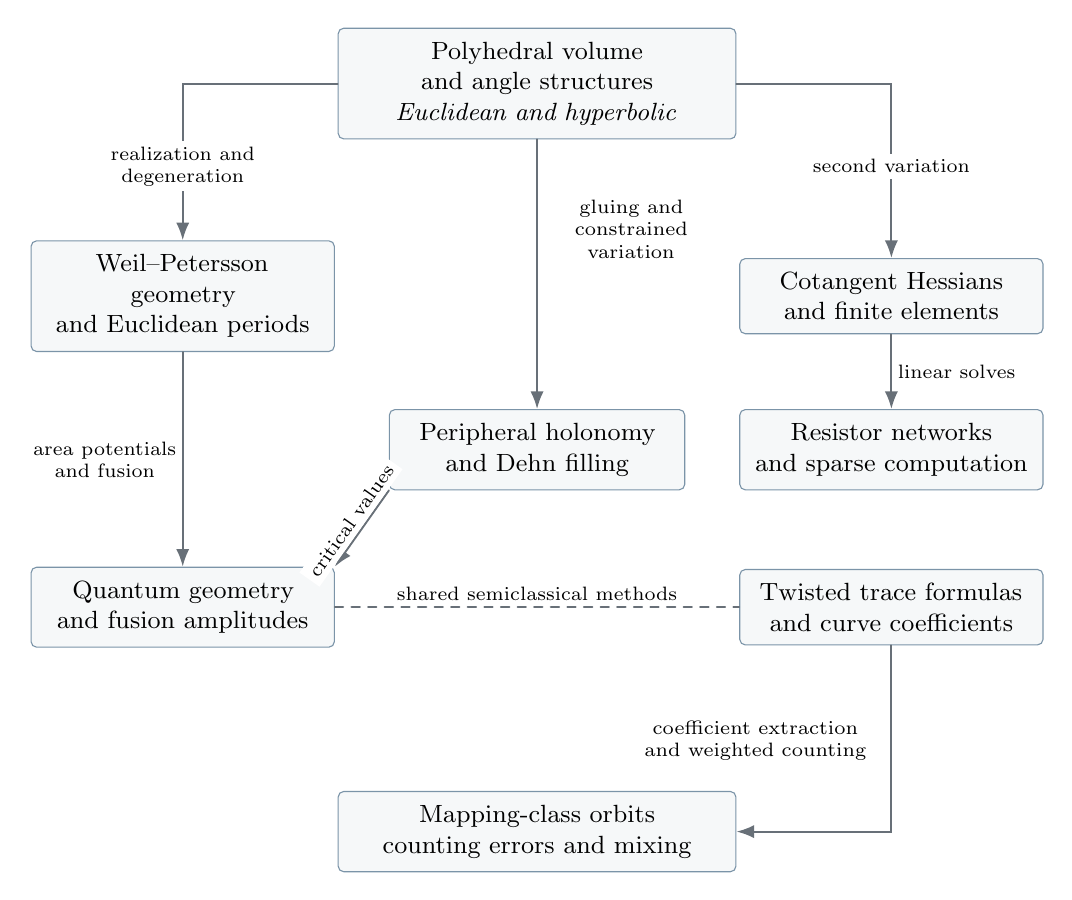
\begin{tikzpicture}[
  font=\small,>=Latex,line cap=round,
  box/.style={draw=mpblue!60,fill=mpblue!4,rounded corners=2pt,
    minimum height=9mm,inner sep=5pt,align=center,text width=3.5cm},
  link/.style={->,draw=mpgray,line width=.75pt},
  lab/.style={font=\scriptsize,fill=white,inner sep=2pt,align=center}]
  \node[box,text width=4.7cm] (poly) at (0,4.4)
    {Polyhedral volume and angle structures\\\textit{Euclidean and hyperbolic}};
  \node[box] (wp) at (-4.5,1.7)
    {Weil--Petersson geometry\\and Euclidean periods};
  \node[box] (fem) at (4.5,1.7)
    {Cotangent Hessians\\and finite elements};
  \node[box,text width=3.4cm] (surgery) at (0,-.25)
    {Peripheral holonomy\\and Dehn filling};
  \node[box] (quantum) at (-4.5,-2.25)
    {Quantum geometry\\and fusion amplitudes};
  \node[box] (complexity) at (4.5,-.25)
    {Resistor networks\\and sparse computation};
  \node[box] (trace) at (4.5,-2.25)
    {Twisted trace formulas\\and curve coefficients};
  \node[box,text width=4.7cm] (count) at (0,-5.1)
    {Mapping-class orbits\\counting errors and mixing};
  \draw[link] (poly.west) -| (wp.north);
  \node[lab] at (-4.5,3.35) {realization and\\degeneration};
  \draw[link] (poly.east) -| (fem.north);
  \node[lab] at (4.5,3.35) {second variation};
  \draw[link] (poly.south)--(surgery.north);
  \node[lab,text width=2.0cm,anchor=west] at (.12,2.55) {gluing and\\constrained\\variation};
  \draw[link] (wp.south)--node[lab,left]{area potentials\\and fusion}(quantum.north);
  \draw[link] (fem.south)--node[lab,right]{linear solves}(complexity.north);
  \draw[link] (surgery.south west)--node[lab,sloped,above]{critical values}(quantum.north east);
  \draw[draw=mpgray,dashed,line width=.75pt] (quantum.east)--node[lab,above]{shared semiclassical methods}(trace.west);
  \draw[link] (trace.south) |- (count.east);
  \node[lab,text width=3cm,anchor=east] at (4.35,-3.95) {coefficient extraction\\and weighted counting};
\end{tikzpicture}
\caption[The geometric and analytic connections]{A guide to the constructions developed in the monograph. Solid
arrows name operations whose domains and hypotheses are stated in the text;
they do not assert equivalences of entire theories. The dashed link records
the use of semiclassical analysis in two different settings: quantum
three-manifold constructions and surface trace formulas. The counting-to-mixing
implications retain their endpoint-weight and nonescape hypotheses.}
\label{fig:mono-connections}
\end{figure}
% END INLINE FIGURE


\subsection*{The principal results}
\addcontentsline{toc}{subsection}{The principal results}

The main conclusions fall into six groups. Their significance lies both
in the individual formulas and in the transfer of information between
the subjects. We give their precise scopes here; the cited sections
contain the hypotheses, proofs, and original sources of the inputs.

\begin{enumerate}[leftmargin=*,label=\textbf{\arabic*.}]
\item \textbf{Polyhedral geometry and moduli volumes.}
The ideal-polyhedral cells give a normalized partition function for
genus-zero WP volumes. For fixed admissible deficit weights, the
final-chamber identity~\eqref{eq:exactWPclassflat} gives an exact class
polynomial, and~\eqref{eq:WPCHvolumeasymptotic} identifies
$2^{-d}V_{\mathrm{CH}}(\mu)$ as the coefficient of $A^d$ in its
small-area volume expansion, with $d=n-3$. This makes
the Euclidean period geometry a computable limit of the hyperbolic
moduli-volume theory. The chamber, labels, and orbifold conventions are
part of the formulas.

\item \textbf{Quantum periods and a uniform degeneration.}
The finite-$b$ identity~\eqref{eq:exactLiouvillecurvature} identifies the
Thurston--Deligne--Mostow form with the logarithmic curvature of a
continued unit-volume Liouville correlation. The four-point residue
calculation determines its fusion matrix and Hermitian area pairing.
Proposition~\ref{prop:regularquantumAiry} gives a separate uniform
Airy theorem, with its first correction, for the specified pole-cleared
tetrahedral integral on the regular one-parameter family.

\item \textbf{Volume optimization, finite elements, and complexity.}
Proposition~\ref{prop:ipolyHessian} identifies the negative volume
Hessian with twice the cotangent stiffness matrix in the disk's
leading--trailing angle coordinates. Equations~\eqref{eq:ipolySchur}
and~\eqref{eq:ipolyForestDeterminant} give its boundary elimination and
rooted-forest determinant. Proposition~\ref{prop:ipolyCompatibility}
supplies the compatible barrier and yields a quantitative path-following
bound after initial centering. The distinction between a fast Laplacian
solve and the full nonlinear realization problem makes the remaining
feasibility, precision, and certification questions explicit.

\item \textbf{Dehn filling through a critical value.}
Proposition~\ref{prop:dehncriticalvalue} identifies the local filling
volume with a holomorphic Legendre critical value as an equality of
analytic germs. Thus every classical long-slope coefficient is fixed,
including the Neumann--Zagier expansion. The inverse volume Hessian
recovers the marked cusp quadratic form, and the Gaussian factor
matches the peripheral factor in torsion surgery. The transfer to a
full quantum invariant is conditional on the representation, cycle,
noncancellation, and competing-sector estimates stated in
Proposition~\ref{prop:dehnquantumconditional}.

\item \textbf{Length-sensitive reconstruction from trace data.}
Proposition~\ref{prop:globaldiagonal} assigns each multicurve an
isolated unit first atom in a length-valued Euler product. A fixed
linear character functional cannot preserve every simple primitive
trace while annihilating every nonsimple trace; the explicit obstruction
is~\eqref{eq:globalobstruction}. Keeping the length and twisting data
therefore matters. The construction supplies exact coefficient objects
and finite isolation bounds, while uniform stability and effective
extraction remain additional analytic questions.

\item \textbf{Effective dynamics and the boundary of sharp counting.}
Theorem~\ref{thm:twopointfullrate} is a converse from a specified weighted
two-endpoint count to mixing, with control of derivative endpoint
weights. Theorem~\ref{thm:markedtorusmixing} gives an explicit global
correlation bound for the marked-torus model of the nonsquare genus-two
$(2,2)$ stratum. The strict-convexity, inverse-flatness, and arithmetic
transfer results then identify the separate geometric and M\"obius
inputs needed for sharp primitive counting. The proposed $O_X(L)$
remainder is a question to be decided, not a conclusion of these results.
\end{enumerate}

\subsection*{The conjectural program}
\addcontentsline{toc}{subsection}{The conjectural program}

The larger quantum-volume problem asks whether controlled local
tetrahedral asymptotics can be assembled into uniform asymptotics of
three-manifold invariants, including Dehn filling. The local critical
value and the Gaussian surgery factor specify two necessary matching
conditions. Global gluing and contour estimates are the next steps.
On the surface side, the coefficient constructions suggest a route from
spectral data to effective connected-curve counting. The weighted
mixing converse specifies the estimate that route would have to produce,
including endpoint regularity and cusp control.

Two further questions join the computational and counting strands to
this program. Can geometric angle bounds and verified linear solves
turn variational existence into useful complexity and certification
theorems beyond the planar model? Can the fine geometry of a torus
norm ball provide the quantitative discrepancy modulus needed to decide
the linear-error question? Section~\ref{sec:questions} states these
targets alongside the other open problems, without assigning an answer
where the evidence does not yet support one.

\subsection*{Structure and routes through the monograph}
\addcontentsline{toc}{subsection}{Structure and routes through the monograph}

The exposition is divided into seven parts. The quantum introduction is
written for geometers who do not assume familiarity with state sums,
recoupling coefficients, conformal blocks, or stationary-phase terminology.
Later calculations can be read after that introduction or reached
directly through the result map above.

\begin{center}
\small
\begin{tabular}{@{}p{.09\textwidth}p{.34\textwidth}p{.50\textwidth}@{}}
\toprule
Part & Subject & Main passage \\
\midrule
I & Polyhedra and moduli measures & Angle cells, WP volume, and Euclidean periods \\[4pt]
II & Variational geometry and computation & Volume Hessians, finite elements, and complexity \\[4pt]
III & Quantum geometry, degeneration, and surgery & Tetrahedral amplitudes, fusion, and peripheral response \\[4pt]
IV & Curves, trace formulas, and quotients & Geodesic identities and length-valued coefficients \\[4pt]
V & Mapping-class dynamics and mixing & Weighted orbit counts and the marked-torus model \\[4pt]
VI & Sharp counting and arithmetic & Flat norm balls, diagnostics, and M\"obius cancellation \\[4pt]
VII & Open problems and conjectural directions & The estimates and geometric comparisons still required \\
\bottomrule
\end{tabular}
\end{center}

A geometric route runs through Parts~I--II and the classical Dehn-filling
calculation in Part~III. A quantum route begins with
Section~\ref{sec:quantumintro}, then follows the period, fusion, Airy, and
surgery comparisons. A surface and spectral route begins with the
geodesic identities in Part~IV and continues through Parts~V--VI.
For computation, Section~\ref{sec:ipolybridge} leads to the inverse-Hessian
response in Section~\ref{sec:dehnresponse} and the counting diagnostics in
Section~\ref{sec:sharpdiagnostics}. These routes share definitions and
normalizations rather than requiring every calculation to be read in order.

\paragraph{Provenance and mathematical status.}
This research monograph grew from a mathematical discussion and includes
both exposition and deductions from the cited literature. The supplied
\texttt{igorrivin/ipoly} snapshot contributes the companion manuscript
and its numerical scripts; Section~\ref{sec:ipolybridge} incorporates its
core variational and computational arguments. Numerical checks are
identified where they occur. A theorem proved for a normalized local
integral, a specified stratum, or a conditional weighted count retains
that scope when it is used elsewhere in the monograph.



\monographpart{Polyhedra and moduli measures}{Polyhedral realization supplies coordinates; the measure comparison turns them into volume formulas. Fixed-deficit Euclidean shapes then reveal a period geometry at the flat limit.}

\section{The volume problem and its normalization}
\label{sec:conventions}

\paragraph{What is being measured?}
A moduli space is a space whose points are geometric objects, with
objects related by the prescribed equivalence regarded as the same point.
Here one point is an oriented hyperbolic surface, considered up to
orientation-preserving isometry that preserves the labels of its ends.
The genus $g$ counts handles; $n$ counts boundary components or cusps.
A geodesic boundary is a closed curve that is straight for the intrinsic
metric. A cusp is a noncompact end with finite area, modeled by a
horoball modulo a translation. ``Unparametrized'' means that a boundary
has a label and a length but no chosen starting point.

The volume of this \emph{space of surfaces} is different from the area
of one surface. For fixed boundary lengths, the latter is already
$2\pi(2g-2+n)$ by Gauss--Bonnet. The volume problem asks how much
room there is to vary the shape. The Weil--Petersson (WP) symplectic
form supplies the measure for that question. A symplectic form is a
closed, nondegenerate alternating two-form; on a space of real
dimension $2d$, its top exterior power $\omega^d/d!$ is the associated
volume form. The integer $d$ below is half the real dimension, and
$\lengths$ abbreviates the ordered list $(L_1,\ldots,L_n)$.

Let $\M_{g,n}(L_1,\ldots,L_n)$ denote the moduli space of oriented hyperbolic
surfaces of genus $g$ with $n$ labeled, unparametrized geodesic boundary
components of prescribed lengths. A zero length denotes a cusp. Throughout,
the curvature is $-1$, the parameters are fixed before taking a volume, and
$2g-2+n>0$. Put
\[
 d=3g-3+n,\qquad
 V_{g,n}(\lengths)=\int_{\M_{g,n}(\lengths)}
                  \frac{\omega_{\WP}^{d}}{d!}.
\]
A useful way to see the dimension is to cut the surface into
\emph{pairs of pants}, meaning spheres with three holes. The
$3g-3+n$ interior cutting curves each contribute a length and a
relative gluing displacement, or twist. These are the
Fenchel--Nielsen coordinates $(\ell_j,\tau_j)$ on the marked
space: a marking identifies the surface topologically with a fixed
reference surface. Forgetting that marking takes the quotient by
mapping classes, that is, orientation-preserving homeomorphisms up
to isotopy. The length--twist coordinates are local coordinates on
moduli, with possible finite symmetries. They do not make the whole
moduli space a rectangular region.

For a pair of pants, $(g,n)=(0,3)$ and $d=0$: the three boundary
lengths determine its metric, so there is no shape parameter left.
For a one-holed torus, $(g,n)=(1,1)$ and $d=1$: cutting one curve
leaves a pair of pants with boundary lengths $(L,\ell,\ell)$,
and gluing the two equal boundaries requires the twist $\tau$.

We use the Fenchel--Nielsen convention
\begin{equation}
 \omega_{\WP}=\sum_{j=1}^{d}\dd\ell_j\wedge\dd\tau_j,
 \qquad \text{one full Dehn twist: }\tau_j\longmapsto\tau_j+\ell_j.
 \label{eq:fn}
\end{equation}
This fixes the scale of the form independently of the convention for
orbifold integration. For comparison with complex coordinates $t_j$, recall that an
infinitesimal change of complex structure can be represented locally
by a \emph{Beltrami differential} $\mu(w)\,\dd\bar w/\dd w$.
The harmonic representative is the canonical representative selected
by the hyperbolic metric; its coefficient $\mu(w)$ is what enters
the following integral. Let
$\mu_j$ be the harmonic Beltrami representative of $\partial/\partial t_j$
and let $H_{j\bar k}=\int_X\mu_j\overline{\mu_k}\,\dd A$ use the curvature
$-1$ area element. Our positive complex convention is
\[
 \omega_{\WP}=i\sum_{j,k}H_{j\bar k}\,\dd t_j\wedge\dd\bar t_k.
\]
The factor is $i$, rather than $i/2$ with the same raw coefficients.
For closed surfaces the conversion is explicit in
\cite[Section 6.1, equation (38)]{KawazumiWP}; that paper writes
$\dd\tau\wedge\dd\ell$, so its twist direction is opposite to ours.
The conical extension used in Section~\ref{sec:flatlimit} retains this
scale; its geometric hypotheses are stated there.

Volumes are orbifold, or stack, volumes: generic ineffective stabilizers are
included. In particular,
\begin{equation}
 V_{0,3}=1,\qquad
 V_{0,4}(\lengths)=2\pi^2+\frac12\sum_{i=1}^4L_i^2,
 \qquad
 V_{1,1}(L)=\frac{L^2+4\pi^2}{48}.
 \label{eq:basevolumes}
\end{equation}
The effective torus volume is twice the last expression. This convention
matters both in unfolding and in the torus--sphere correspondence; see
Do--Norbury~\cite{DoNorbury} and Section~\ref{sec:torussphere}.
More generally, a generic ineffective stabilizer of order $h$ divides the
effective volume by $h$ without rescaling the local two-form. Rescaling
$\omega_{\WP}$ by a constant $c$ instead multiplies a $2d$-dimensional
volume by $c^d$. These are separate normalization operations.

The orbifold convention can be understood in a finite quotient chart.
If a finite symmetry group of order $h$ acts on a parameter region,
its orbifold integral is the integral upstairs divided by $h$.
This includes elements that act trivially on the parameters, called
\emph{ineffective} symmetries. On the one-holed torus the generic
elliptic involution contributes such a factor of two. Thus the
stack volume at $L=0$ is $\pi^2/12$, whereas the effective quotient
volume is $\pi^2/6$. This changes the counting of objects with
symmetries; it does not replace the local form $\dd\ell\wedge\dd\tau$
by half that form.

The original geometric proposal has three separate ingredients:
\begin{enumerate}
 \item realize an intrinsic surface by a canonical convex polyhedron;
 \item describe the allowed polyhedra by cells, ideally linear polytopes;
 \item identify the pullback of $\omega_{\WP}^{d}/d!$ on each cell.
\end{enumerate}
The realization and the cell decomposition identify the integration domain.
They do not, by themselves, identify its measure. In the ideal genus-zero
case the measure comparison is particularly favorable; in the hyperideal
case a useful local density is still available, but it is generally no longer
constant in the natural angle variables.

There are also two different cross-ratios in the four-point problem.
The cross-ratio is the complex parameter obtained by taking three
ordered points on the Riemann sphere to $0,1,\infty$ by a M\"obius
transformation and recording the image of the fourth, with the
ordering fixed. Four
ideal vertices on $\partial\HH^3$ have an \emph{ambient} cross-ratio. The
intrinsic metric on the polyhedral boundary has a conformal uniformization,
and its four punctures have a \emph{conformal} cross-ratio. The realization
theorem relates the two parameter spaces, but these two numerical coordinates
are not generally equal. Keeping them distinct is essential to the first
explicit integral below.

The computational companion in
\texttt{experiments/normalizations/README.md} records exact finite checks
of the determinants, factors, and low-dimensional intersection formulas
used in Sections~\ref{sec:conventions}--\ref{sec:flatlimit} and
Appendix~\ref{app:fricke}; its machine-readable output is
\path{artifacts/normalizations/result.json}. These fixtures check
algebraic consequences and conventions. They do not prove the cited
realization, measure-comparison, or convergence theorems.


\section{Ideal polyhedra, angle cells, and a partition function}
\label{sec:idealcells}

The aim is to replace an integral over surfaces by ordinary integrals
over finitely many regions of angle assignments. Two issues have to
be settled: which assignments come from polyhedra, and what density
they carry. An \emph{ideal} vertex lies on the sphere at infinity of
hyperbolic three-space. It has no finite distance from an interior
point, but a polyhedron with ideal vertices can have finite volume.
Its boundary metric has a cusp at each vertex.

\subsection{The geometric parametrization}

In the polyhedral cell discussion take $n\ge4$; the three-ended sphere is
the zero-dimensional pants base case.

The \emph{dual graph} has a vertex for each face of the polyhedron
and an edge crossing each original edge. A dual face encircles one
original vertex. The orientation supplies a cyclic order of edges
at every dual vertex; a graph with these cyclic orders is a
\emph{ribbon graph}. Thickening its edges to narrow strips recovers
an oriented surface with boundary. Here the complementary faces
are labeled by the punctures. A simple circuit is a closed edge
path with no repeated vertices except its starting/ending vertex.

Rivin's intrinsic realization theorem identifies a complete finite-area
hyperbolic metric on an $n$-punctured sphere with the boundary metric of a
convex ideal polyhedron, uniquely up to ambient isometry. Flat doubles of
ideal polygons occur as limiting configurations~\cite{RivinIntrinsic}.
For oriented moduli one retains the orientation of the boundary and uses
orientation-preserving equivalences.

Fix a combinatorial polyhedron and write $\theta_e$ for its exterior dihedral
angles. In the dual graph, the ideal conditions are
\begin{align}
 &0<\theta_e<\pi,\label{eq:rivinangles1}\\
 &\sum_{e\in\partial f}\theta_e=2\pi
       &&\text{for every dual face }f,\label{eq:rivinangles2}\\
 &\sum_{e\in C}\theta_e>2\pi
       &&\text{for every simple dual circuit not bounding a face.}
       \label{eq:rivinangles3}
\end{align}
Here the dual graph is the planar, $3$-connected graph of a convex
polyhedron, with its oriented embedding fixed. With these hypotheses, these
are Rivin's characterization~\cite{RivinAngles}. Thus the admissible angle
assignments form an open convex polytope in an affine subspace. Generic
polyhedra have triangular faces; their dual maps are trivalent and have
$3n-6$ edges. The $n$ perimeter conditions are independent: their matrix
is the unsigned vertex--edge incidence matrix of the primal triangulation.
A row relation assigns numbers $c_v$ with $c_v+c_w=0$ across every edge;
a triangular face forces its three numbers to vanish, and connectedness
forces all of them to vanish. The dimension is therefore $2n-6$.

An edge of the dual graph has metric length $\theta_e$. The resulting metric
map has face perimeters $2\pi$ and no short nonfacial circuit. This is the
genus-zero instance of a $2\pi$-irreducible metric map. It gives the precise
combinatorial object behind the proposed sum over polyhedral types.

For example, an ideal tetrahedron has six edges and four ideal
vertices. At the regular tetrahedron each interior dihedral angle
is $\pi/3$, hence each exterior angle $\theta_e$ is $2\pi/3$.
The three angles around a dual face add to $2\pi$; a nonfacial
four-edge circuit has sum $8\pi/3>2\pi$. The four independent
linear perimeter equations leave $6-4=2$ free parameters, agreeing
with the real dimension of the four-punctured-sphere moduli space.
These are lengths of the \emph{dual metric graph}, measured in
radians; they are not the infinite lengths of the original ideal edges.

\subsection{A normalized cell integral}

A sum over combinatorial types must avoid counting the same labeled,
oriented object several times, and an integral on a constraint surface
must specify its measure. The first issue produces the automorphism
factor below. The second can already be seen in the toy constraint
$x+y=L$ with $x,y>0$:
\[
 \int_{x,y>0} f(x,y)\,\delta(x+y-L)\,\dd x\,\dd y
   =\int_0^L f(x,L-x)\,\dd x.
\]
Here $\delta$ is the Dirac delta, characterized by
$\int f(u)\delta(u-a)\,\dd u=f(a)$.
The measure on this line is $\dd x$, whereas its Euclidean arc length
is $\sqrt2\,\dd x$. Disintegration means choosing the measure on
each fiber so that integration over fibers and then over the constraint
value recovers the original ambient integral. This distinction is the
reason for retaining the determinant in the graph formula.

For a dual ribbon graph $G$ with labeled faces, define its constrained
Lebesgue measure by disintegrating $\prod_e\dd\theta_e$ with respect to the
face-perimeter map. Symbolically, at perimeters $\boldsymbol\alpha$,
\begin{equation}
 \dd\nu_G(\boldsymbol\alpha)=
 \left(\prod_{e\in E(G)}\dd\theta_e\right)
 \left(\prod_{i=1}^{n}
 \delta\left(\sum_{e\in\partial f_i}\theta_e-\alpha_i\right)\right).
 \label{eq:deltameasure}
\end{equation}
An edge is counted with its boundary multiplicity. This notation specifies
a disintegrated measure, rather than Euclidean hypersurface measure with an
unstated coarea factor.
Concretely, let $P$ be the perimeter matrix and split the edge coordinates
as $(u,v)$ so that the square $n\times n$ block $P_v$ is invertible.
On the fiber $P_u u+P_vv=\boldsymbol\alpha$, the measure is
\[
 \dd\nu_G=\frac{|\dd u_1\cdots\dd u_{2n-6}|}{|\det P_v|},
 \qquad v=P_v^{-1}(\boldsymbol\alpha-P_u u).
\]
Thus deleting $n$ dependent edge variables without this determinant would
change the normalization.

The ideal cell description is known to give a volume calculation, beyond
the possibility suggested by the realization theorem. Charbonnier--David--Eynard
compare the angle measure with the WP form through lambda lengths
\cite[Section 3.2]{CDE}. In Budd's normalization of metric-map volume,
\begin{equation}
 \boxed{
 V_{0,n}(0,\ldots,0)=
 2^{n-2}\sum_{[G]}\frac{1}{|\Aut(G)|}
 \int_{\mathcal P_G}\dd\nu_G(2\pi,\ldots,2\pi).}
 \label{eq:polyhedralpartition}
\end{equation}
Here $\mathcal P_G$ imposes positivity and irreducibility, $G$ ranges over
oriented trivalent maps with labeled faces, and automorphisms preserve this
data. Nontrivalent strata have zero volume. Budd gives this interpretation
and the normalization explicitly~\cite[Section 1.3]{Budd}.
Equivalently, his rooted-map measure gives each root weight
$1/(2|E(G)|)$; summing the $2|E(G)|/|\Aut(G)|$ rooted versions gives
the displayed unrooted weight. Reversing the cyclic orders is not an
allowed equivalence of oriented maps.

Thus there is a genuine partition function over polyhedral combinatorial
types. Formula~\eqref{eq:polyhedralpartition} is a finite cellwise integral
at fixed $n$; it is not a sum over geodesics. The factors in it encode three
choices that should never be suppressed: labels, orientation, and the
normalization of the constrained measure. Section~\ref{sec:tetrahedron}
checks them directly for $n=4$.

\subsection{The string-theoretic connection}

Saadi--Zwiebach's closed-string construction uses equal-perimeter polyhedral
diagrams and quadratic differentials~\cite{SaadiZwiebach}. Zwiebach's
minimal-area formulation imposes a lower bound $2\pi$ on nontrivial closed
curves and uses uniqueness to control the covering of moduli space
\cite{Zwiebach}. These give a concrete historical counterpart to the
suggestion that such cells should be used for integration.

Several identifications nevertheless require care. A quadratic differential is locally an expression $q=\varphi(w)\,\dd w^2$
whose transformation rule makes $|q|$ a well-defined flat metric away
from its zeros and poles. A Jenkins--Strebel differential is a special
one whose regular horizontal trajectories form cylinders of closed
curves. Their boundaries make a metric ribbon graph. Conversely a
suitable metric ribbon graph can be thickened by these flat cylinders
into a surface.
A hyperbolic polyhedron has an intrinsic hyperbolic boundary metric and also
extrinsic dual data. These constructions may share the same combinatorial
and length description without giving the same metric or the same conformal
coordinate on moduli. Likewise, a string amplitude includes its specified
integrand; a decomposition used for string integration does not automatically
select the WP measure. Equation~\eqref{eq:polyhedralpartition} uses an
explicit measure comparison, not just the common vocabulary of polyhedra.


\section{The ideal tetrahedron: an explicit volume integral}
\label{sec:tetrahedron}

\subsection{Lambda lengths and the ambient cross-ratio}

Take the four labeled ideal vertices to be $0,1,\infty,z$, where
$z=x+iy\in\CC\setminus\{0,1\}$. For $y\ne0$ their convex hull is a genuine
ideal tetrahedron. The two half-planes describe its two orientation types.

For a decorated ideal triangulation, set $\lambda_e=e^{\delta_e/2}$, where
$\delta_e$ is the signed distance between the chosen horocycles along the
edge. An overall fixed multiplier in the definition of $\lambda$ does not
change its logarithmic differential. With cyclically ordered edge lengths
$a,b,c$ on each oriented triangle, Penner's formula in convention
\eqref{eq:fn} is
\begin{equation}
 \omega_{\WP}=-2\sum_{\triangle}
 \bigl(\dd\log a\wedge\dd\log b+
       \dd\log b\wedge\dd\log c+
       \dd\log c\wedge\dd\log a\bigr).
 \label{eq:penner}
\end{equation}
This is a form on decorated Teichm\"uller space that descends after forgetting
the horocycles~\cite{Penner}; its magnitude agrees with the cuspidal limit
of Mondello's arc-coordinate formula~\cite{MondelloBoundary}.

The four decorations can be chosen so that
\begin{equation}
 \lambda_{0\infty}=\lambda_{1\infty}=\lambda_{z\infty}
 =\lambda_{01}=1,
 \qquad \lambda_{0z}=r=|z|,\quad\lambda_{1z}=s=|1-z|.
 \label{eq:lambdagauge}
\end{equation}
For example, use equal Euclidean diameters for the three finite horospheres
in the upper-half-space model and adjust their common scale together with
the horosphere at infinity. The usual formula for the signed distance then
gives~\eqref{eq:lambdagauge}.
One may take diameter $1$ for each finite horosphere and height $1$ at
infinity. The finite-edge formula is then
$\lambda_{ij}=|z_i-z_j|$, and each edge to infinity has lambda length $1$.
Overlapping horospheres cause no problem: the distances are signed, and
smaller embedded decorations can first be chosen and then rescaled.

Every face containing $\infty$ has at most one varying lambda length, so its
contribution in~\eqref{eq:penner} vanishes in this section of the decoration
bundle. The remaining face has lengths $1,r,s$. Consequently the positive
WP measure is
\begin{equation}
 \boxed{
 \dV=2\abs{\dd\log r\wedge\dd\log s}
      =\frac{2|y|}{|z|^2|1-z|^2}\,\dd x\,\dd y.}
 \label{eq:tetdensity}
\end{equation}
The Jacobian calculation is elementary:
\[
 \dd\log r=\frac{x\,\dd x+y\,\dd y}{r^2},\qquad
 \dd\log s=\frac{(x-1)\,\dd x+y\,\dd y}{s^2}.
\]
Their wedge is $y\,\dd x\wedge\dd y/(r^2s^2)$.

\subsection{Integration in angle coordinates}

For $y>0$, let $A,B,C$ be the interior angles of the Euclidean triangle
with vertices $0,1,z$. They satisfy
\[
 A>0,\quad B>0,\quad C>0,\quad A+B+C=\pi.
\]
They are also the three interior dihedral angles of the ideal tetrahedron,
each repeated on the opposite edge. Direct differentiation gives
\[
 \abs{\dd A\wedge\dd B}
   =\frac{y}{r^2s^2}\,\dd x\,\dd y,
 \qquad\text{hence}\qquad
 \dV=2\,\dd A\,\dd B.
\]
One orientation sheet therefore contributes
\begin{equation}
 \int_{\substack{A>0,\ B>0\\A+B<\pi}}2\,\dd A\,\dd B=\pi^2.
 \label{eq:onecell}
\end{equation}
Including the other sheet gives the promised direct calculation:
\begin{equation}
 \boxed{V_{0,4}=2\pi^2.}
 \label{eq:v04direct}
\end{equation}
The real configurations form the flat locus and contribute zero two-dimensional
WP measure.

There is also a useful check on~\eqref{eq:polyhedralpartition}. In a
tetrahedral angle cell, the four perimeter equations force opposite exterior
angles to be equal, with three values $a,b,c$ satisfying $a+b+c=2\pi$.
To see the disintegration factor explicitly, order the edges as
$(01,02,03,12,13,23)$, keep $a=\theta_{01}$ and $b=\theta_{02}$,
and eliminate the last four variables. The corresponding perimeter minor is
\[
 \begin{pmatrix}
 1&0&0&0\\0&1&1&0\\0&1&0&1\\1&0&1&1
 \end{pmatrix},\qquad \det=-2.
\]
It gives $(\theta_{03},\theta_{12},\theta_{13},\theta_{23})
=(2\pi-a-b,2\pi-a-b,b,a)$ and the measure
$\frac12|\dd a\,\dd b|$. Up to permuting the three angle names,
$a=\pi-A$ and $b=\pi-B$, so this is
$\frac12\dd A\,\dd B$. There are two oriented cells, each with trivial
label-preserving automorphism group. The factor $2^{4-2}=4$ in
\eqref{eq:polyhedralpartition} converts their total map volume $\pi^2/2$
to $2\pi^2$.

\subsection{What happens at the punctures of the parameter plane?}

Finite volume requires integrability, not pointwise decay of a coordinate
density. Near $z=0$, write $z=\rho e^{i\vartheta}$. Then
\[
 \frac{2|y|}{|z|^2|1-z|^2}
 =\frac{2|\sin\vartheta|}{\rho}\,(1+O(\rho)),
 \qquad \dd x\,\dd y=\rho\,\dd\rho\,\dd\vartheta.
\]
The singularity is integrable. The same is true at $1$. At infinity the
density is $O(|z|^{-3})$, again integrable against Euclidean area. Thus the
requested decay is best formulated as a condition on the measure, not on
its density without its coordinate area element.

\begin{remark}[The coordinate is not conformal]
Formula~\eqref{eq:tetdensity} is the pullback to the ambient ideal-vertex
coordinate. It is not a formula for WP measure in the intrinsic conformal
cross-ratio. In particular, its vanishing on the real locus does not mean
that the WP form degenerates at an ordinary interior point of moduli space.
The polyhedral parametrization is not a smooth coordinate across that locus.
The Delaunay literature also distinguishes the embedding coordinate from
uniformization~\cite[Section 3.3.1]{CDE}.
\end{remark}

Nor do two ordinary closed angle triangles describe the full topology of
the compactification without additional data. As $y\downarrow0$ with
$0<x<1$, two of the triangle angles tend to zero and the third to $\pi$,
independently of $x$. A whole family of flat quadrilaterals approaches one
angle-simplex vertex. Retaining that modulus requires a refinement of the
boundary, such as a real blow-up. This has no effect on the integral over
the open cells.


\section{Hyperideal polyhedra: an actual local integrand}
\label{sec:hyperideal}

\subsection{From vertices to orthogeodesic lengths}

A strictly hyperideal vertex lies outside the closed ball in the projective
model, while every edge meets the ball. Its polar plane cuts off the vertex.
After all such truncations, the original faces form a bordered hyperbolic
surface; the truncation polygons give its geodesic boundaries. Ideal vertices
can be included by a limiting procedure and give cusps.

For a hyperideal tetrahedron choose unit spacelike representatives
$v_1,\ldots,v_4$ in Minkowski space of signature $(3,1)$. Choose their signs
so that they represent the vertices in one projective affine chart and
have negative pairwise inner products. Set
\begin{equation}
 q_{ij}=-\langle v_i,v_j\rangle=\cosh a_{ij}>1.
 \label{eq:qvertices}
\end{equation}
Here $a_{ij}$ is the length of the original edge between the two polar
truncation planes. It is an orthogeodesic of the intrinsic bordered surface.
The six $a_{ij}$ specify the vertex configuration up to ambient isometry on
the admissible tetrahedral domain.

Let $b_i^{jk}$ be the side of the truncation triangle at vertex $i$ that lies
in the original face $ijk$. The right-angled hexagon cosine rule gives
\begin{equation}
 \cosh b_i^{jk}=
 \frac{\cosh a_{ij}\cosh a_{ik}+\cosh a_{jk}}
      {\sinh a_{ij}\sinh a_{ik}},
 \qquad
 L_i=\sum_{\{j,k\}\subset\{1,2,3,4\}\setminus\{i\}}b_i^{jk}.
 \label{eq:truncationlengths}
\end{equation}
The four $L_i$ are intrinsic boundary lengths. They are not the sums of the
exterior dihedral angles around the hyperideal vertices.

These formulas also describe the domain concretely. The Gram matrix
\begin{equation}
 G_{ii}=1,\qquad G_{ij}=-q_{ij}\quad(i\ne j)
 \label{eq:gram}
\end{equation}
must have signature $(3,1)$. With all $q_{ij}>1$, the strict tetrahedral
condition is $\det G<0$. Indeed, each $3\times3$ principal determinant is
$1-q_{ij}^2-q_{ik}^2-q_{jk}^2-2q_{ij}q_{ik}q_{jk}<0$.
The trace and a negative $2\times2$ principal determinant then show that
this block has signature $(2,1)$. Interlacing and $\det G<0$ give
signature $(3,1)$ for $G$.

There is also a direct check of the geometric inequalities used below.
At vertex $i$, put
\[
 u_j=\frac{v_j+q_{ij}v_i}{\sqrt{q_{ij}^2-1}}\quad(j\ne i).
\]
These are unit timelike vectors in $v_i^\perp$, with
$-\langle u_j,u_k\rangle=\cosh b_i^{jk}>1$, so they lie in the same
sheet of its hyperboloid. Their Gram determinant is
$\det G/\prod_{j\ne i}(q_{ij}^2-1)<0$ by the Schur complement.
Thus they are three noncollinear points in $\HH^2$: their pairwise
distances $b_i^{jk}$ form a genuine triangle and satisfy strict triangle
inequalities. Conversely a Gram realization with this signature lies in
a common affine chart: a positive eigenvector for the largest eigenvalue
of $I-G$ gives a timelike positive combination of the $v_i$ whose inner
products with all four are negative. Every projective edge meets the ball
because $\langle v_i+v_j,v_i+v_j\rangle=2-2q_{ij}<0$.

It is possible to glue right-angled hexagons from a wider set of positive
arc-length assignments and obtain a valid intrinsic bordered surface. Such
arcs need not be the edges of its convex hyperideal realization. Thus the
polyhedral domain must be imposed when the purpose is to integrate a
canonical polyhedral cell.

\subsection{The WP density on a fixed-boundary leaf}

Mondello's Poisson formula for arc lengths has the boundary kernel
\begin{equation}
 K_L(s)=\frac{\sinh(L/2-s)}{\sinh(L/2)},\qquad 0<s<L.
 \label{eq:boundarykernel}
\end{equation}
For two different arcs $e,f$, the bracket in convention~\eqref{eq:fn} is
one half the sum of these kernels over their common boundary endpoints,
with oriented boundary distances from the endpoint of $e$ to that of $f$.
Changing the order changes the sign, since $K_L(L-s)=-K_L(s)$.
The factor $1/2$ results from evaluating the ordered wedge sum in
\cite[Theorem 4.1]{MondelloBoundary}.
That theorem is stated for a compact surface with strictly positive
geodesic boundaries and a maximal disjoint orthogeodesic arc system.
Boundary lengths are Casimirs of the Poisson tensor; inversion is performed
only after restricting to a fixed-boundary leaf. The matrix in all six
tetrahedral arc lengths is therefore not the matrix to invert.

Restrict now to the two-dimensional leaf where $L_1,\ldots,L_4$ are fixed.
The arcs $a_{12},a_{13}$ share just the boundary at vertex $1$, and the
relevant distance is $b=b_1^{23}$, up to orientation. Inverting the
two-dimensional Poisson tensor gives
\begin{equation}
 \boxed{
 \dV=
 2\frac{\sinh(L_1/2)}{\sinh(L_1/2-b_1^{23})}
 \abs{\dd a_{12}\wedge\dd a_{13}}.}
 \label{eq:hyperidealdensity}
\end{equation}
Since the three truncation sides form a genuine triangle,
$b_1^{23}<L_1/2$. Thus the denominator is positive, the bracket is nonzero,
and these two arc lengths are local coordinates on this leaf.

Formula~\eqref{eq:hyperidealdensity} is an actual expression for the volume
integrand in terms of the hyperideal geometry. Its remaining variables are
functions on the fixed-$L$ leaf; they cannot be held independently fixed
while $a_{12},a_{13}$ vary.

For an expression directly in the vertex Gram entries, put
\[
 D=q_{12}^2+q_{13}^2+q_{23}^2+2q_{12}q_{13}q_{23}-1.
\]
Equation~\eqref{eq:truncationlengths} gives
\[
 \cosh b=\frac{q_{12}q_{13}+q_{23}}
                   {\sqrt{q_{12}^2-1}\sqrt{q_{13}^2-1}},\qquad
 \sinh b=\frac{\sqrt D}
                   {\sqrt{q_{12}^2-1}\sqrt{q_{13}^2-1}}.
\]
Substituting in~\eqref{eq:hyperidealdensity} and using
$\dd q_{ij}=\sinh a_{ij}\,\dd a_{ij}$ yields
\begin{equation}
 \boxed{
 \dV=
 \frac{2\abs{\dd q_{12}\wedge\dd q_{13}}}
 {q_{12}q_{13}+q_{23}-\coth(L_1/2)\sqrt D}.}
 \label{eq:gramdensity}
\end{equation}
The positivity follows from the same truncation-triangle inequality.
For a concrete normalization check, take $q_{ij}=2$ for every edge.
Then $G=3I-2\mathbf1\mathbf1^t$ has determinant $-135$,
$a_{ij}=b_i^{jk}=a=\operatorname{arcosh}2$, and $L_i=3a$.
The kernel is $K_{3a}(a)=1/5$, so the bracket is $1/10$ and
\eqref{eq:hyperidealdensity} has coefficient $10$. In Gram coordinates
$D=27$ and $\coth(3a/2)=3\sqrt3/5$, giving coefficient $10/3$ in
\eqref{eq:gramdensity}, exactly as $\sinh^2a=3$ requires.
This evaluates a local density at one admissible point; it does not solve
the fixed-boundary equations throughout a cell.

The cusp limit requires renormalization. As a positive boundary shrinks,
the raw distances to its truncation plane diverge; subtract the endpoint
terms corresponding to a chosen limiting horocycle before comparing with
lambda lengths. If $s/L\to\rho$, the kernel itself has the regular limit
$K_L(s)\to1-2\rho$. A fixed-perimeter horocycle gauge is different from
the four-unit-lambda gauge in~\eqref{eq:lambdagauge}; changing that gauge
changes coordinate Jacobians, while preserving the descended WP form.
This is the cuspidal limiting procedure underlying
\cite[Theorem 4.5]{MondelloBoundary}.

\subsection{General cells and what remains to integrate}

The same procedure applies to any arc system. On a fixed-boundary leaf,
choose independent arc coordinates $x_1,\ldots,x_{2d}$ and form the
antisymmetric matrix
\[
 B_{ef}=\{x_e,x_f\}_{\WP}.
\]
If it is nonsingular, then
\begin{equation}
 \boxed{
 \dV=\frac{|\dd x_1\cdots\dd x_{2d}|}{|\Pf B|}
       =\frac{|\dd x_1\cdots\dd x_{2d}|}{\sqrt{\det B}}.}
 \label{eq:pfaffiandensity}
\end{equation}
This is simply the top exterior power of the inverse Poisson matrix. It
turns a local arc-bracket formula into a local volume formula in every
dimension.

Bao--Bonahon's angle characterization assumes a planar $3$-connected dual
graph, $0<\theta_e<\pi$, circuit sums at least $2\pi$ with equality
only around ideal vertices, and sums greater than $\pi$ on embedded paths
joining distinct vertices of one dual face without lying in its boundary
\cite[Theorems 1--2]{BaoBonahon}. The path condition must not be dropped
when passing from ideal to hyperideal cells.
For a complete genus-zero hyperbolic metric with finitely many cusps and
infinite-area ends, the global realization theorem gives a unique
finite-vertex convex generalized hyperbolic polyhedron, up to congruence.
This is the case without finite cone singularities of the precise
restatement in~\cite[Theorem 1.1]{FillastreMetrics}; Section 1.3 there
attributes its proof to Schlenker~\cite{Schlenker}. For a bordered surface,
one attaches funnels and then truncates along the polar planes.
Rivin's intrinsic theorem supplies
ideal existence and generalized uniqueness~\cite[Theorems 1.1--1.3]{RivinIntrinsic}.
The local Gram and Poisson calculations above are independent of invoking
this global existence theorem.

For fixed $L_i$, however, the angle cell is cut out further by the nonlinear
equations~\eqref{eq:truncationlengths}. The local density is therefore more
complicated than in the ideal case. The known total
\[
 V_{0,4}(L_1,L_2,L_3,L_4)=2\pi^2+\tfrac12\sum_iL_i^2
\]
provides a stringent target for a direct evaluation of these cell integrals.
No such full hyperideal evaluation is carried out in this monograph.

Budd's metric-map polynomials obey, for $g=0,1$,
\begin{equation}
 V_{g,n}^{(2\pi)}(\alpha_1,\ldots,\alpha_n)
 =2^{2-2g-n}V_{g,n}\bigl(\sqrt{\alpha_1^2-4\pi^2},\ldots,
                         \sqrt{\alpha_n^2-4\pi^2}\bigr).
 \label{eq:buddidentity}
\end{equation}
This does not extend to $g\ge2$. Nor does the displayed substitution describe
the actual relation between hyperideal angle perimeters and truncation
boundary lengths~\cite[Corollary 2 and Section 1.3]{Budd}. It is useful
evidence of a connection, with a separate geometric question behind it.

\subsection{A further tree-coordinate result}

There is now an additional concrete integration route for genus zero with
a distinguished cusp. Budd--Meeusen--Zonneveld construct a spine bijection
from a full-measure subset to explicitly decorated tree polytopes
\cite[Theorem 1]{BMZ}. Writing $m$ for the total number of ends, their
statement has the form
\begin{equation}
 \M_{0,m}^{\circ}(0,\lengths)\ \longleftrightarrow\
 \bigsqcup_{\mathfrak t}\mathcal A_{\mathfrak t}(\lengths),
 \qquad
 \dV=2^{m-3}\,\dd^{\,2m-6}u_{\mathfrak t}.
 \label{eq:treevolume}
\end{equation}
Thus its volume is a finite sum of ordinary polytope volumes, with this
specified constant density. Their construction uses spine and tree
coordinates rather than the Bao--Bonahon hyperideal angle cells. It
requires an origin cusp.
In~\eqref{eq:treevolume}, $u_{\mathfrak t}$ means the independent coordinates
used in~\cite[equation (5)]{BMZ}: two angles at each trivalent inner
vertex and all but the last entry in each of the two boundary simplices
of size $L_i/2$. It is not Euclidean hypersurface measure on the redundant
coordinate space. With $m=n+1$ in that paper, its factor $2^{n-2}$ is
precisely $2^{m-3}$ here.

Zonneveld's sequel removes that restriction using decompositions into
half-tight cylinders~\cite[Theorem 3]{Zonneveld}. For positive boundary
lengths, with a selected pair satisfying $L_1<L_2$, it gives a full-measure
bijection to tree and double-tree cells and identifies their WP measures.
The latter cells include a gluing length and a twist parameter. The resulting
finite integrations compute the general genus-zero volume polynomials;
equal-length volume values follow by continuity. These are further direct
combinatorial integrations, but they do not identify the spine cells with
the hyperideal dihedral-angle cells. The direct evaluation in those
polyhedral coordinates remains a distinct calculation proposed here.


\section{Boundary lengths, cone angles, and continuation}
\label{sec:cones}

\subsection{Fixed signature and the polynomial chamber}

Allow $a$ cone points with opening angles $\theta_1,\ldots,\theta_a$ and
$b$ geodesic boundary components with lengths $L_1,\ldots,L_b$, including
zero lengths for cusps. Thus $n=a+b$ and $d=3g-3+n$. The area is
\begin{equation}
 \operatorname{Area}(X)=2\pi(2g-2+n)-\sum_{i=1}^{a}\theta_i>0.
 \label{eq:gb}
\end{equation}
There is no separate puncture parameter in the volume polynomial: a cusp
is represented by $L=0$, or equivalently by cone opening zero.

Use the logarithmic tautological class
$\kappa_1=\pi_*(\psi_{n+1}^2)$ on $\MM_{g,n}$. The fixed-boundary WP class,
continued to cone parameters, is
\begin{equation}
 \Omega_0=2\pi^2\kappa_1+\frac12\sum_{j=1}^{b}L_j^2\psi_j
                          -\frac12\sum_{i=1}^{a}\theta_i^2\psi_i.
 \label{eq:wpclass}
\end{equation}
The labels in the two sums are understood to be disjoint. In its geometric
validity chamber,
\begin{equation}
 V_{g,n}(\lengths,i\angles)=\frac1{d!}
                          \int_{\MM_{g,n}}\Omega_0^d.
 \label{eq:intersectionvolume}
\end{equation}
The boundary formula follows from the symplectic-reduction/intersection
description of WP volumes~\cite{MirzIntersection}; imaginary lengths
$L=i\theta$ account for the minus sign~\cite{DoNorbury}.

For mixed positive boundaries and cone points, a safe geometric regime is
$0\le\theta_i<\pi$. For pure cone/cusp surfaces, the uncorrected formula
holds in the larger chamber where every pair of openings sums to less than
$2\pi$~\cite[Theorem 1.1 and Corollary 1.2]{AnagnostouNorbury}.
In both statements the area condition~\eqref{eq:gb} and the prescribed
labels remain part of the hypotheses. Polynomial evaluation outside these
ranges is always algebraically defined, but requires a separate geometric
justification. In particular, a single cone of arbitrary
opening below $2\pi$, with only cusps as the other ends, does not create a
cone-collision wall.

For example, on $\MM_{0,4}$ one has
$\int\kappa_1=\int\psi_i=1$, so
\begin{equation}
 V_{0,4}(\lengths,i\angles)
 =2\pi^2+\frac12\sum L_j^2-\frac12\sum\theta_i^2
 \label{eq:mixedv04}
\end{equation}
whenever this chamber formula applies. On $\MM_{1,1}$,
$\int\kappa_1=\int\psi_1=1/24$, giving the torus normalization in
\eqref{eq:basevolumes} and its one-cone continuation.

\subsection{Pure cone/cusp volumes beyond the first chamber}

For $0\le\theta_i<2\pi$, put
\[
 w_i=1-\frac{\theta_i}{2\pi},\qquad
 \Phi_S=\sum_{i\in S}\theta_i-2\pi(|S|-1),\qquad u_+=\max(u,0).
\]
Assume $2g-2+\sum_iw_i>0$. A collision of the marked points in $S$ is
allowed in the weighted compactification when $\sum_{i\in S}w_i\le1$.
The class pulled back to ordinary Deligne--Mumford space is
\begin{equation}
 \boxed{
 \Omega_{\angles}=2\pi^2\kappa_1-\frac12\sum_i\theta_i^2\psi_i
      +\frac12\sum_S(\Phi_S)_+^2\,\delta_{0:S}.}
 \label{eq:wallclass}
\end{equation}
The sum runs over stable rational-tail divisors, with $|S|\ge2$. The
geometric volume is $\int\Omega_{\angles}^{d}/d!$. This is the
wall-crossing class of Anagnostou--Mullane--Norbury
\cite[Definitions 2.12--2.13 and Lemma 2.14]{AMN}, also expressed in the
cone-volume formulation of Eberhardt--Turiaci~\cite{ET}.
Here stability means that both components of the nodal curve are stable
in ordinary DM space; in genus zero this requires also $|S^c|\ge2$.
All classes in~\eqref{eq:wallclass}, including $\kappa_1$ and $\psi_i$,
are on that ordinary compactification. They must not be replaced by
weighted-space classes without applying the reduction pullback.

For completeness, the coefficient follows immediately from the weighted
formula: its normalized correction is
$(1-\sum_{i\in S}w_i)^2\delta_{0:S}$, and multiplication by $2\pi^2$
gives $(\Phi_S)^2/2$. If $r$ is the reduction to the relevant weighted
compactification, then $r$ is proper and birational. Therefore
$r_*[\MM_{g,n}]=[\MM_{g,\mathbf w}]$, and the projection formula justifies
integrating the top power of the pulled-back class on ordinary DM space.
On a wall $\Phi_S=0$ the added term vanishes. The formula therefore
extends continuously from adjacent chambers, although its polynomial
expression changes across the wall. In dimension greater than one the
top power includes products and self-intersections of the boundary
divisors; adding their coefficients as scalar volume corrections would
not compute the volume.

In genus zero $\delta_{0:S}=\delta_{0:S^c}$. There is no positive-term
double counting in~\eqref{eq:wallclass}: stability gives $\sum_iw_i>2$,
so both $S$ and its complement cannot have weight at most one.

For four labeled cone/cusp points the formula becomes particularly simple:
\begin{equation}
 \boxed{
 V_{0,4}(i\angles)=2\pi^2-\frac12\sum_{i=1}^4\theta_i^2
 +\frac12\sum_{1\le i<j\le4}(\theta_i+\theta_j-2\pi)_+^2.}
 \label{eq:conev04}
\end{equation}
For openings $(0,0,3\pi/2,3\pi/2)$, the area is positive but the uncorrected
polynomial gives $-\pi^2/4$. The single active correction contributes
$\pi^2/2$, giving the actual positive volume $\pi^2/4$. This example
pinpoints the failure of unrestricted polynomial continuation.

With a positive geodesic boundary and a cone opening greater than $\pi$,
additional degenerations can occur when the cone approaches that boundary.
Anagnostou--Norbury exhibit such a nonnodal degeneration
when the positive boundary length is sufficiently large
\cite[Lemma 2.10]{AnagnostouNorbury}. We consequently assert the full
wall formula here for pure cones/cusps, and the preceding small-cone regime
for arbitrary mixed positive boundaries. An unrestricted mixed-signature
geometric theorem would require its own hypotheses and boundary analysis.

\subsection{What continuation means for compact polyhedra}

The boundary of a compact convex hyperbolic polyhedron has intrinsic cone
opening $\theta_v$ equal to the sum of its face angles at $v$; its singular
curvature is $2\pi-\theta_v$. Neither is an individual dihedral angle.
Thus the substitution $L\mapsto i\theta$ concerns an intrinsic holonomy
parameter. It is not a literal substitution of arbitrary hyperideal vertex
coordinates by compact ones.

At a local algebraic level the continuation is natural. For example,
\begin{equation}
 K_L(s)=\frac{\sinh(L/2-s)}{\sinh(L/2)}
 \quad\longmapsto\quad
 \frac{\sin(\theta/2-\alpha)}{\sin(\theta/2)}
 \quad\text{under }(L,s)=(i\theta,i\alpha).
 \label{eq:kernelcontinuation}
\end{equation}
Trace and Gram formulas have analogous analytic continuations. Recovering
a real geometric volume also requires a real geometric domain, a valid
coordinate chart, and the appropriate collision chamber. The polynomial
example above shows why these cannot be inferred from the formal algebra.


\section{Equal parameters and the torus--sphere correspondence}
\label{sec:torussphere}

The familiar punctured correspondence extends geometrically to equal
positive boundaries. Let $Q(c^4)$ be a four-holed sphere with all four
boundary lengths $c$, and let $T(2c)$ be a one-holed torus with boundary
length $2c$. The relevant construction is through a common orbifold:
\begin{equation}
 T(2c)\xrightarrow{\;2:1\;}
 O(c;\pi,\pi,\pi)
 \xleftarrow{\;4:1\;}Q(c,c,c,c).
 \label{eq:commonorbifold}
\end{equation}
The middle surface is a sphere with one geodesic boundary and three
angle-$\pi$ orbifold points. The torus quotient uses its elliptic
involution; the sphere quotient uses its Klein-four symmetry. This works
for every $c>0$ and limits to the cusped case~\cite[Section 3]{HuTan}.

A matching simple curve on $T$ covers an arc between two orbifold points
twice; its counterpart on $Q$ covers that arc four times. Thus
\begin{equation}
 \ell_Q=2\ell_T.
 \label{eq:lengthtorussphere}
\end{equation}
The construction gives a correspondence of simple-curve classes, not only
an agreement of dimension or of volume polynomials.

WP forms scale by the degree of a local-isometric covering on a family of
lifted metrics. This follows from naturality of the Goldman symplectic
pairing: its surface integral is multiplied by the covering degree.
On the common marked orbifold family,
\[
 \omega_T=2\omega_O,\qquad \omega_Q=4\omega_O,
 \qquad\text{so}\qquad\omega_Q=2\omega_T.
\]
This comparison takes place before dividing by mapping classes. Branch
points are cone points of the quotient, so the maps are local isometries
in the orbifold sense; their orders $2$ and $4$ multiply the same integral
pairing. The statement does not involve varying the boundary length $c$.
Generically the equal-boundary sphere has its Klein-four isometry group.
There are $4!/4=6$ inequivalent ways to label its boundaries. The torus has
its generic elliptic involution, which acts ineffectively on Teichm\"uller
space. The Klein-four transformations permute the four sphere boundaries
freely and transitively, so none survives after all four labels are fixed.
The generic degree from labeled spheres to the effective torus moduli
space is therefore $6$, and the local area ratio is $2$. Consequently
\begin{equation}
 \boxed{
 V_{0,4}(c,c,c,c)=12V_{1,1}^{\rm eff}(2c)
                =24V_{1,1}^{\rm stack}(2c).}
 \label{eq:voltorussphere}
\end{equation}
Indeed, $24((2c)^2+4\pi^2)/48=2\pi^2+2c^2$, as required by
\eqref{eq:basevolumes}. Exceptional extra automorphisms are accounted for
by orbifold integration. Forgetting the ineffective torus involution is
the source of a common factor-of-two discrepancy.

The cone analogue can be constructed directly. For $0<\phi<\pi$, the
elliptic quotient of a torus with one cone opening $2\phi$ is a sphere
with openings $(\phi,\pi,\pi,\pi)$. Its Klein-four cover branched over
the three angle-$\pi$ points has four openings equal to $\phi$. Uniqueness
of conical uniformization makes the conformal symmetries isometries.
The same degree and labeling argument gives
\begin{equation}
 V_{0,4}(i\phi,i\phi,i\phi,i\phi)
   =2\pi^2-2\phi^2=24V_{1,1}(2i\phi).
 \label{eq:conetorus}
\end{equation}
The common quotient cone surface has area $\pi-\phi$, so $\phi<\pi$ is exactly the
hyperbolic range. There are no collision corrections in this equal-cone
sphere chamber.
The torus has one cone opening $2\phi<2\pi$ and no other noncuspidal
ends, so its polynomial evaluation is covered by the single-cone regime
of Section~\ref{sec:cones}. Thus both sides of~\eqref{eq:conetorus} are
geometric volumes in the stated interval. The endpoint $\phi=\pi$ has
zero area and is a limit, not an additional hyperbolic moduli space.

This correspondence does not assert a direct unbranched degree-two map
from the four-holed sphere to the one-holed torus. The common orbifold and
its two different covering degrees are the precise geometric statement.


\section{Euclidean shapes and Deligne--Mostow periods}
\label{sec:thurstonDM}

\subsection{The fixed-curvature leaf at the Euclidean end}

Fix $n\ge4$ and real numbers
\begin{equation}
 0<\mu_i<1,\qquad \sum_{i=1}^n\mu_i=2.
 \label{eq:flatweights}
\end{equation}
The Euclidean cone opening at the $i$th marked point is
$2\pi(1-\mu_i)$, so $2\pi\mu_i$ is its curvature deficit. A conformal
sphere $X$ with these marked points carries a unique such flat metric up
to multiplication by a positive constant. In a coordinate with all marks
finite it has the explicit form
\begin{equation}
 g_{\mathrm E,\mu}=C\prod_i|w-p_i|^{-2\mu_i}|\dd w|^2.
 \label{eq:flatconemetric}
\end{equation}
The sum condition makes infinity a regular point. Near $p_i$, radial
integration gives a cone of opening $2\pi(1-\mu_i)$. Thus the space of
oriented, labeled Euclidean cone spheres with these deficits, up to
similarity, has underlying complex manifold $\M_{0,n}$.

Alexandrov realization identifies these metrics with convex Euclidean
polyhedral surfaces, allowing doubled planar polygons. This is the
fixed-deficit space on which Thurston constructs his complex hyperbolic
metric~\cite{ThurstonShapes,Fillastre}. The qualification ``fixed
deficits'' is essential: all Euclidean polyhedra with $n$ vertices, up
to similarity, form a space of real dimension $3n-7$, whereas the
fixed-deficit leaf has real dimension $2n-6$. The full space of compact
hyperbolic $n$-vertex polyhedra has dimension $3n-6$; its fixed-cone-angle
leaves again have dimension $2n-6$. The ideal locus has dimension $2n-6$.
These dimension counts apply on the generic strata; changes of
combinatorics and flattened realizations require the usual cell structure.


% BEGIN INLINE FIGURE: 02_polyhedral_regimes.tex
\begin{figure}[htbp]
\centering
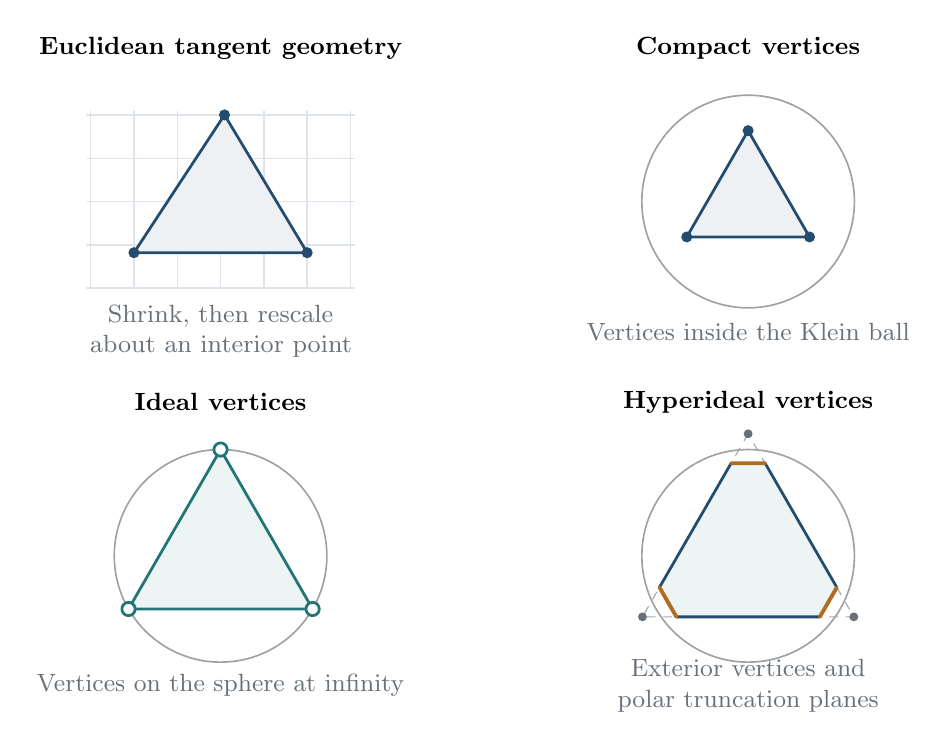
\begin{tikzpicture}[font=\small,line cap=round,line join=round]
  \begin{scope}[shift={(-3.35,2.15)}]
    \node[align=center,font=\bfseries\small] at (0,1.95) {Euclidean tangent geometry};
    \draw[mpblue!15,line width=.5pt] (-1.7,-1.1) grid[step=.55] (1.7,1.15);
    \filldraw[fill=mpblue!8,draw=mpblue,line width=1pt]
      (-1.1,-.65)--(1.1,-.65)--(.05,1.1)--cycle;
    \foreach \p in {(-1.1,-.65),(1.1,-.65),(.05,1.1)}\fill[mpblue] \p circle (2pt);
    \node[align=center,text width=4.5cm,text=mpgray] at (0,-1.65)
      {Shrink, then rescale\\about an interior point};
  \end{scope}
  \begin{scope}[shift={(3.35,2.15)}]
    \node[font=\bfseries\small] at (0,1.95) {Compact vertices};
    \draw[mpgray!65,line width=.6pt] (0,0) circle (1.35);
    \filldraw[fill=mpblue!8,draw=mpblue,line width=1pt]
      (90:.9)--(210:.9)--(330:.9)--cycle;
    \foreach \a in {90,210,330}\fill[mpblue] (\a:.9) circle (2pt);
    \node[text=mpgray] at (0,-1.65) {Vertices inside the Klein ball};
  \end{scope}
  \begin{scope}[shift={(-3.35,-2.35)}]
    \node[font=\bfseries\small] at (0,1.95) {Ideal vertices};
    \draw[mpgray!65,line width=.6pt] (0,0) circle (1.35);
    \filldraw[fill=mpteal!8,draw=mpteal,line width=1pt]
      (90:1.35)--(210:1.35)--(330:1.35)--cycle;
    \foreach \a in {90,210,330}\filldraw[fill=white,draw=mpteal,line width=1pt] (\a:1.35) circle (2.4pt);
    \node[text=mpgray] at (0,-1.65) {Vertices on the sphere at infinity};
  \end{scope}
  \begin{scope}[shift={(3.35,-2.35)}]
    \node[font=\bfseries\small] at (0,1.95) {Hyperideal vertices};
    \draw[mpgray!65,line width=.6pt] (0,0) circle (1.35);
    \draw[mpgray!60,dashed] (90:1.55)--(210:1.55)--(330:1.55)--cycle;
    \fill[mpteal!8]
      (-.21604075,1.17580645)--(-1.12629863,-.40080645)--(-.91025788,-.775)
      --(.91025788,-.775)--(1.12629863,-.40080645)--(.21604075,1.17580645)--cycle;
    \draw[mpblue,line width=1pt]
      (-.21604075,1.17580645)--(-1.12629863,-.40080645)
      (-.91025788,-.775)--(.91025788,-.775)
      (1.12629863,-.40080645)--(.21604075,1.17580645);
    \draw[mpochre,line width=1.4pt]
      (-.21604075,1.17580645)--(.21604075,1.17580645)
      (-1.12629863,-.40080645)--(-.91025788,-.775)
      (.91025788,-.775)--(1.12629863,-.40080645);
    \foreach \a in {90,210,330}\fill[mpgray] (\a:1.55) circle (1.6pt);
    \node[text=mpgray,align=center] at (0,-1.65)
      {Exterior vertices and\\polar truncation planes};
  \end{scope}
\end{tikzpicture}
\caption[Euclidean, compact, ideal, and hyperideal regimes]{Local pictures for the geometric regimes. The three Klein-model
drawings are planar sections illustrating the location of vertices;
the ochre segments are polar truncations in the hyperideal case.
The Euclidean picture represents a tangent-scale limit after shrinking
and rescaling. These drawings do not assert a single global deformation
through all four regimes with arbitrary prescribed data.}
\label{fig:mono-polyhedral-regimes}
\end{figure}
% END INLINE FIGURE

\subsection{The same periods describe hypergeometric functions and developed edges}

Define the multivalued differential
\begin{equation}
 \eta_p(w)=\prod_i(w-p_i)^{-\mu_i}\,\dd w.
 \label{eq:DMdifferential}
\end{equation}
Its branches differ by unit complex numbers. It therefore defines a
twisted cohomology class for a rank-one unitary local system on the
punctured sphere. The relevant twisted cohomology space has complex
dimension $n-2$, and its Hermitian intersection form $H$ has signature
$(1,n-3)$, with the convention that the class of $\eta_p$ has positive
norm. In a local basis of twisted cycles or regularized relative arcs,
the coordinates
\begin{equation}
 Z_j(p)=\int_{\gamma_j}\eta_p
 \label{eq:DMperiods}
\end{equation}
are the hypergeometric periods of Deligne--Mostow~\cite{DeligneMostow}.
Projectivizing their positive line gives a local map to
$\mathbb{CH}^{n-3}$. Analytic continuation produces projective unitary
monodromy.

Thurston's Euclidean construction uses exactly the same coordinates.
The local developing map is
\[
 F(w)=\int^w\eta_p.
\]
Hence a developed edge vector is an integral of $\eta_p$ along the
corresponding arc. Cutting along a tree produces a Euclidean polygon
whose edge vectors are periods, and whose area is the Hermitian form
in these periods. Normalize $H$ by this area pairing. Then, more
intrinsically,
\begin{equation}
 \mathcal A(p)=\frac{i}{2}\int_{\mathbb P^1}\eta_p\wedge\overline{\eta_p}
             =H(Z(p),Z(p)).
 \label{eq:DMarea}
\end{equation}
Multiplication of all periods by a nonzero complex number changes only
the scale and rotation of the developed surface. Quotienting by this
action is precisely the projectivization in the Deligne--Mostow
construction.

Thus the connection is an equality of geometric structures: the
hypergeometric periods are the developed edge vectors, and the
Hermitian intersection pairing is the area pairing. Kojima proves that
the two constructions, with labels retained, are canonically isometric
\cite[Lemmas 4.1--4.2 and Theorem 4.3]{Kojima}. The scalar used for
the Hermitian intersection pairing varies between sources; fixing it
by~\eqref{eq:DMarea} removes that ambiguity, and a constant scalar
does not change the projective metric. Throughout this monograph the complex hyperbolic
metric has \emph{holomorphic sectional curvature $-1$}. Its K\"ahler
form, in the preceding local period coordinates, is
\begin{equation}
 \omega_{\mathrm{CH}}=-2i\,\partial\bar\partial\log\mathcal A.
 \label{eq:CHpotential}
\end{equation}
A holomorphic change of local scale for $\eta_p$ does not affect this
form. On a complex line in the ball, $\mathcal A=1-|z|^2$ gives
$\dd s^2=4|\dd z|^2/(1-|z|^2)^2$, which checks the curvature
normalization directly. A curvature-$-4$ convention would divide the form by $4$ and
the volume in complex dimension $d$ by $4^d$.

If the weights are rational, choose their least common denominator
$q$, so $\mu_i=m_i/q$. The compact normalization of the connected cyclic
cover
\[
 y^q=\prod_i(w-p_i)^{m_i}
\]
makes $\eta_p=\dd w/y$ a single-valued holomorphic differential. Under
the deck transformation $y\mapsto e^{2\pi i/q}y$ it has eigenvalue
$e^{-2\pi i/q}$. The corresponding eigenspace in the ordinary
cohomology of this cover realizes the twisted cohomology. This gives a
further useful interpretation in terms of periods of algebraic curves;
it does not require the monodromy group to be a lattice.

\subsection{Collision angles and the lattice conditions}

Suppose two marks of total weight $\mu_i+\mu_j<1$ collide, with local
separation $\delta$, while the other marks remain distinct and away
from the collision. After fixing a branch, rescaling the integration variable in their
vanishing period gives
\begin{equation}
 Z_{ij}(\delta)=C\delta^{\,1-\mu_i-\mu_j}(1+O(\delta)),\qquad C\ne0.
 \label{eq:vanishingperiod}
\end{equation}
The transverse complex hyperbolic cone angle is consequently
$2\pi(1-\mu_i-\mu_j)$. Deligne--Mostow's condition INT is
\begin{equation}
 (1-\mu_i-\mu_j)^{-1}\in\ZZ_{>0}
 \quad\text{for every pair with }\mu_i+\mu_j<1.
 \label{eq:INT}
\end{equation}
Under this condition the completion by finite-distance collisions has
orbifold universal cover $\mathbb{CH}^{n-3}$, and the monodromy is a
lattice. Cusps remain at infinite distance. For the half-integral
variant, fix a block of equal-weight marks and permit every permutation
within that block. Interchanging two of its marks sends $\delta$ to
$-\delta$; the quotient coordinate is $\delta^2$, so the transverse
angle is halved.
Mostow's $\Sigma$INT condition is therefore
\[
 (1-\mu_i-\mu_j)^{-1}\in
 \begin{cases}
 \tfrac12\ZZ_{>0},&i,j\text{ both in the specified block},\\
 \ZZ_{>0},&\text{otherwise},
 \end{cases}
 \qquad \mu_i+\mu_j<1.
\]
Mostow's theorem gives an orbifold uniformization for that permutation
quotient~\cite[Sections 1--3]{MostowHalfIntegral}; the labeled completion
need not itself be an orbifold when a reciprocal is a nonintegral
half-integer. Thurston gives the corresponding criterion when all
equal-weight permutations are allowed~\cite[Theorem 0.2]{ThurstonShapes}.

When $\mu_i+\mu_j=1$, the collision is a cusp rather than a finite
cone-angle divisor; logarithmic periods and parabolic monodromy enter.
For general real weights satisfying~\eqref{eq:flatweights}, the local
complex hyperbolic geometry and its finite volume still exist
\cite[Theorem 0.2]{ThurstonShapes}. One
must not infer a lattice quotient for arbitrary weights. Conversely,
INT and $\Sigma$INT are the classical sufficient uniformization
conditions, not a claim to classify every exceptional discrete
hypergeometric monodromy group. Our volumes retain all labels; a
quotient by allowed equal-weight permutations changes the quotient
and the volume factors.

\subsection{Four equal deficits and elliptic periods}

For $n=4$ and $\mu_i=1/2$, put the marks at $0,1,z,\infty$. Then
\begin{equation}
 \eta=\frac{\dd w}{\sqrt{w(w-1)(w-z)}},\qquad
 E_z:\ y^2=w(w-1)(w-z).
 \label{eq:ellipticDM}
\end{equation}
The Euclidean cone sphere is the flat pillowcase quotient of this
elliptic curve. The ratio of two periods gives a coordinate
$\tau\in\HH$. For $0<z<1$, one choice is
\begin{equation}
 \tau(z)=i\frac{K(1-z)}{K(z)},\qquad
 K(z)=\int_0^{\pi/2}\frac{\dd u}{\sqrt{1-z\sin^2u}}.
 \label{eq:ellipticperiodratio}
\end{equation}
Here $z$ is the elliptic parameter, not its square root. The inverse
map is the modular lambda function. Projective monodromy is
$\mathrm P\Gamma(2)=\Gamma(2)/\{\pm I\}$, and the labeled moduli
space is the thrice-punctured
sphere with curvature-$-1$ area $2\pi$. The action of $S_4$ on the
cross-ratio has the Klein four-group as its kernel. Its effective
quotient therefore has degree $6$, and is the modular orbifold of
area $\pi/3$; dividing the labeled area by $24$ would instead retain
the ineffective stabilizer
\cite[Example 2.1 and Section 5]{Kojima}. This is the flat
endpoint of the equal-angle torus--sphere correspondence in
Section~\ref{sec:torussphere}.


\section{From ideal polyhedra to the Euclidean limit of WP geometry}
\label{sec:flatlimit}

\subsection{A prescribed intrinsic interpolation}

For the weights in~\eqref{eq:flatweights}, define
\begin{equation}
 \theta_i(t)=2\pi t(1-\mu_i),\qquad
 a_i(t)=1-t(1-\mu_i),\qquad 0\le t<1.
 \label{eq:anglepath}
\end{equation}
Hold the marked conformal sphere $X\in\M_{0,n}$ fixed, and let $g_t(X)$
be its curvature-$-1$ cone metric with these openings. Its area is
\begin{equation}
 A_t=2\pi\left(\sum_i a_i(t)-2\right)
    =2\pi(n-2)(1-t).
 \label{eq:areapath}
\end{equation}
At $t=0$ the metric is the complete cusped metric, realized by an ideal
polyhedron, including doubled ideal polygons. For $0<t<1$ it is a positive-deficit hyperbolic cone metric,
realized by a compact convex hyperbolic polyhedron, with flattened
realizations included when necessary. The realization results are
reviewed in~\cite{Fillastre}; the ideal and generalized settings are
treated in~\cite{RivinIntrinsic,Schlenker}.

Normalize to unit area:
\begin{equation}
 \widehat g_t=A_t^{-1}g_t,
 \qquad \operatorname{Area}(\widehat g_t)=1,
 \qquad K(\widehat g_t)=-A_t.
 \label{eq:unitareanormalization}
\end{equation}
The unit-area uniformization and local deformation results of
Mazzeo--Weiss give the flat limit
\begin{equation}
 \widehat g_t(X)\longrightarrow g_{\mathrm E,\mu}(X)
 \quad (t\to1),
 \label{eq:flatmetriclimit}
\end{equation}
with the Euclidean metric normalized to area one. Here their angle
parameters are $\beta_i(t)=-a_i(t)\in(-1,0)$ near $t=1$, and
$\chi(S^2)+\sum_i\beta_i(t)=-D(1-t)\le0$, where $D=n-2$.
Thus their nonpositive-curvature existence and uniqueness theorem
applies, including the flat endpoint. Their smooth local slices give
convergence away from the cone points and uniform conic estimates
after a local trivialization fixing the marks
\cite[Theorem 1, Section 6.1, and Proposition 16]{MazzeoWeiss}.
This is a deduction along the specified path; it is local over
moduli where the marks remain separated.

This constructs a family of complex fixed-angle leaves with two
geometric endpoints: cusped hyperbolic surfaces/ideal polyhedra, and
flat cone spheres/Euclidean shapes. It does not assign a single
complex structure to all angle variables in the full real space of
hyperbolic polyhedra. Nor is it generally radial scaling of a fixed
Euclidean vertex configuration in the Klein ball. Such radial scaling
makes all vertices ideal simultaneously only for a cospherical
configuration. Every nondegenerate Euclidean tetrahedron is
cospherical, but its radial path still need not preserve $X$ or
the angle path~\eqref{eq:anglepath}.

\subsection{The normalized local WP form}

The scale of the WP form can be seen directly from the cotangent
pairing. Write $w=x+iy$ and $g_t=\rho_t|\dd w|^2$. For
$q=\varphi\,\dd w^2$ and $r=\psi\,\dd w^2$, the raw coefficient
pairing is
\[
 Q_t(q,r)=\int_X\frac{\varphi\overline\psi}{\rho_t}\,\dd x\,\dd y.
\]
Since $\rho_t=A_t\widehat\rho_t$, the rescaled cometric $A_tQ_t$
has a finite flat limit. A quadratic differential has at most a
simple pole at a marked point, while
$\widehat\rho_t\to\rho_{\mathrm E}$ with
$\rho_{\mathrm E}=c_i(w)|w|^{-2\mu_i}$ for a smooth positive local
factor $c_i$. The limiting integrand is
$O(|w|^{2\mu_i-2})\,\dd x\,\dd y$, which is integrable because
$\mu_i>0$. On a compact subset of a coordinate chart in moduli, the
conic estimates bound the nearby integrands by
$C|w|^{2m-2}\,\dd x\,\dd y$ for some $m>0$. Dominated convergence
therefore gives locally uniform convergence of the pairing matrices.
Their flat limit is positive definite, so matrix inversion gives a
tangent metric and a K\"ahler form of order $A_t$. No assertion here
allows the marked points to collide or a weight to tend to zero.

To determine the constant, use the raw tangent coefficients
$G_{j\bar k}(g)=\int_X\nu_j\overline{\nu_k}\,\dd A_g$, where
$\nu_j$ is the harmonic Beltrami representative of a complex coordinate
vector $\partial/\partial z_j$. Our FN normalization is
$\omega_{\WP}=i\sum G_{j\bar k}\,\dd z_j\wedge\dd\bar z_k$,
as fixed in Section~\ref{sec:conventions}; equivalently, on real
tangent vectors it is $-2\operatorname{Im}G$
\cite[Section 6.1, equation (38)]{KawazumiWP}.
Wang's period-variation calculation, translated to the positive area
pairing~\eqref{eq:DMarea}, gives
\[
 -\frac{\partial^2\log\mathcal A}{\partial z_j\partial\bar z_k}
  =\frac{G_{j\bar k}(g_{\mathrm E})}
         {\operatorname{Area}(g_{\mathrm E})}.
\]
Indeed, the component of the variation of $[\eta]$ orthogonal to
$[\eta]$ is represented by $\nu_j\mathbin{\lrcorner}\eta$; its
negative Hermitian norm divided by $H(\eta,\eta)$ is the displayed
area average. This is the normalization-independent content of
\cite[Theorem 1.2.1 and Section 4.4]{WangFlatWP}. Inserting
\eqref{eq:CHpotential} now gives
\begin{equation}
 \boxed{\quad A_t^{-1}\omega_{\WP,t}
       \longrightarrow\frac12\omega_{\mathrm{CH},\mu}.\quad}
 \label{eq:localWPCHlimit}
\end{equation}
The convergence is of form coefficients locally uniformly on the
open moduli space. The factor is also checked independently by the
class calculation below. This conclusion combines the two cited
inputs with the specified FN convention; neither source states this
hyperbolic-to-flat limit verbatim. Local convergence on a noncompact
moduli space alone does not justify convergence of total volumes.

\subsection{The class calculation and an exact final-chamber polynomial}

Put $d=n-3$, $D=n-2$, and $\mu_I=\sum_{i\in I}\mu_i$. Let
$\delta_I=\delta_{I^c}$ denote the divisor of the stable bipartition
$I\mid I^c$. Define the real divisor class
\begin{equation}
 B_\mu=\frac12\left(
   -\sum_i\mu_i\psi_i+
   \sum_{\{I,I^c\}}\min(\mu_I,\mu_{I^c})\delta_I\right),
 \label{eq:CHclassB}
\end{equation}
where the second sum counts each unordered stable bipartition once.
Use the real compactification class on the ordinary
Deligne--Mumford compactification, defined at balanced weights by
continuity. Its normalization and volume formula are
\begin{equation}
 [\omega_{\mathrm{CH},\mu}]=4\pi B_\mu,\qquad
 V_{\mathrm{CH}}(\mu)=\frac{(4\pi)^d}{d!}
                     \int_{\MM_{0,n}}B_\mu^d.
 \label{eq:CHintersection}
\end{equation}
Away from balanced weights, Koziarz--Nguyen's normalized form
$\Omega_\mu$ represents $B_\mu$ as a closed current. Their
Section 7.3 gives the divisor class, and Section 7.4 converts it
to curvature $-1$ by
$\omega_{\mathrm{CH},\mu}=4\pi\Omega_\mu$
\cite[Theorem 1.1 and Sections 7.3--7.4]{KoziarzNguyen}.
Their direct metric/current analysis excludes subsets $\mu_I=1$;
at these balanced weights the displayed divisor class and volume
formula are understood by continuity, as explained in their
Remark 1.3. The volume on the left is the finite volume of the
open labeled moduli space, with no permutation quotient.

Let $\varepsilon=1-t$, $r_i=1-\mu_i$, and
$r_I=\sum_{i\in I}r_i=|I|-\mu_I$. Then
$a_i=\mu_i+\varepsilon r_i$ and $A=2\pi D\varepsilon$. Write
$\mathcal L_\mu$ for the stable subsets with $\mu_I<1$, each light
side counted once. For sufficiently small positive $\varepsilon$,
these are precisely the light subsets in the adjacent hyperbolic
chamber. Subsets with $\mu_I=1$ are \emph{not} light along this path.
Define
\begin{equation}
 \boxed{\quad
 \Xi_\mu=\frac{1}{2D^2}\left(
 -\sum_i(1-\mu_i)^2\psi_i+
 \sum_{I\in\mathcal L_\mu}(|I|-\mu_I)^2\delta_I\right).
 \quad}
 \label{eq:Xiclass}
\end{equation}

\begin{proposition}[A deduction from the two compactification formulas]
In the final chamber of the path~\eqref{eq:anglepath},
\begin{align}
 [\omega_{\WP}(A)]
   &=\frac A2[\omega_{\mathrm{CH},\mu}]+A^2\Xi_\mu,
       \label{eq:exactWPclassflat}\\
 V_{\WP}(A)
   &=\frac{A^d}{d!}\int_{\MM_{0,n}}
       \left(\frac12[\omega_{\mathrm{CH},\mu}]+A\Xi_\mu\right)^d.
       \label{eq:exactWPvolumeflat}
\end{align}
In particular,
\begin{equation}
 \boxed{\quad
 V_{\WP}(A)=2^{-d}A^d V_{\mathrm{CH}}(\mu)+O(A^{d+1}).
 \quad}
 \label{eq:WPCHvolumeasymptotic}
\end{equation}
The volume in~\eqref{eq:exactWPvolumeflat} is exactly a polynomial in
$A$ with possible degrees $d,d+1,\ldots,2d$ within that chamber.
\end{proposition}

\begin{proof}
In terms of deficit weights, the pulled-back WP class
\eqref{eq:wallclass}, divided by $2\pi^2$, is
\[
 \beta(a)=\kappa_1-\sum_i(1-a_i)^2\psi_i+
           \sum_{a_I<1}(1-a_I)^2\delta_I.
\]
Here all collision sums run over stable subsets, so
$2\le |I|\le n-2$; since $\sum a_i>2$, both sides of a
bipartition cannot be light. We verify the two needed endpoint
identities on the ordinary universal curve
$\pi:\mathcal C\to\MM_{0,n}$. Write $\Gamma_i$ for its sections,
$K=K_{\mathcal C/\MM_{0,n}}+\sum_i\Gamma_i$, and $F_I$ for
the vertical component over $\delta_I$ carrying the marks in $I$.
For the fixed final-chamber list $\mathcal L_\mu$, set
\[
 \Lambda(a)=K-\sum_i(1-a_i)\Gamma_i
                  -\sum_{I\in\mathcal L_\mu}(1-a_I)F_I.
\]
The universal-curve intersections used in
\cite[Section 8.4]{KoziarzNguyen} are
\[
 \begin{gathered}
 \pi_*K^2=\kappa_1,\qquad K\Gamma_i=0,\qquad
 \pi_*(\Gamma_i^2)=-\psi_i,\qquad \Gamma_i\Gamma_j=0\ (i\ne j),\\
 \pi_*(KF_I)=(|I|-1)\delta_I,\qquad
 \pi_*(F_IF_J)=-\mathbf1_{I=J}\delta_I,\qquad
 \pi_*(\Gamma_iF_I)=\mathbf1_{i\in I}\delta_I.
 \end{gathered}
\]
Consequently $\pi_*\Lambda(a)^2=\beta(a)$. For example, with
$c=1-a_I$, the coefficient of $\delta_I$ in this square is
$-2c(|I|-1)+2c\sum_{i\in I}(1-a_i)-c^2=c^2$; this checks
the sign of the vertical correction.

For rational flat weights away from balanced subsets, the corrected
divisor $\Lambda(\mu)$ is fiberwise trivial and is the pullback of
Koziarz--Nguyen's extended period-line class $B_\mu$
\cite[Sections 8.1 and 8.4]{KoziarzNguyen}. All coefficients extend
continuously to real weights and to balanced subsets, whose vertical
coefficient $1-\mu_I$ vanishes. Hence
$\Lambda(\mu)=\pi^*B_\mu$ as real divisor classes throughout
\eqref{eq:flatweights}. Along our fixed chamber,
\[
 \Lambda(\mu+\varepsilon r)=\pi^*B_\mu+\varepsilon R,
 \qquad R=\sum_i r_i\Gamma_i+\sum_{I\in\mathcal L_\mu}r_IF_I,
 \qquad \pi_*R=\sum_i r_i=D.
\]
The projection formula now gives
$\pi_*\Lambda(\mu)^2=0$ and first-order term
$2\varepsilon D B_\mu$. Equivalently,
\begin{align*}
 \beta(\mu)&=0,\\
 \sum_i r_i^2\psi_i-
   \sum_{I\in\mathcal L_\mu}(1-\mu_I)r_I\delta_I&=D B_\mu.
\end{align*}
These are general class identities obtained by pushforward; finite
intersection checks are supplementary.

Expanding the quadratic expression for $\beta$ now gives
\[
 \beta(\mu+\varepsilon r)=2\varepsilon D B_\mu+
 \varepsilon^2\left(-\sum_i r_i^2\psi_i+
                \sum_{I\in\mathcal L_\mu}r_I^2\delta_I\right).
\]
Multiplication by $2\pi^2$, followed by
$A=2\pi D\varepsilon$ and~\eqref{eq:CHintersection}, proves
\eqref{eq:exactWPclassflat}. The WP intersection-volume theorem
\cite{AMN} proves~\eqref{eq:exactWPvolumeflat}; its leading term is
\eqref{eq:WPCHvolumeasymptotic}.
\end{proof}

Within the original parameter interval $0<\varepsilon\le1$, the
open final chamber is
\begin{equation}
 0<\varepsilon<\varepsilon_*,\qquad
 \varepsilon_*=
 \begin{cases}
 \displaystyle\min_{I\in\mathcal L_\mu}
                \frac{1-\mu_I}{|I|-\mu_I},&\mathcal L_\mu\ne\varnothing,\\
 1,&\mathcal L_\mu=\varnothing.
 \end{cases}
 \label{eq:finalchamberwidth}
\end{equation}
When the light-subset set is empty, the same polynomial also holds
at the cusped endpoint $\varepsilon=1$. At a collision wall the
vanishing correction makes the adjacent volume polynomials agree,
but the strict inequality specifies which chamber supplies the
coefficients. Along the full
path, a stable subset crosses its wall at
$t_I=(|I|-1)/(|I|-\mu_I)$ when $\mu_I<1$. Thus the ideal-to-flat
volume is piecewise polynomial, even though the final expansion is
an exact polynomial.

\subsection{Examples and nonuniformity at balanced weights}

With four equal weights $\mu_i=1/2$, all openings are $\pi t$, and
there are no active collision corrections for $t<1$. Thus
\begin{equation}
 V_{\WP}(t)=2\pi^2(1-t^2),\qquad A=4\pi(1-t),\qquad
 V_{\WP}(A)=\pi A-\frac{A^2}{8}.
 \label{eq:equalflatvolume}
\end{equation}
Here $\int B_\mu=1/2$, $V_{\mathrm{CH}}=2\pi$, and
$\int\Xi_\mu=-1/8$, checking all constants directly.

For $\mu=(3/10,2/5,3/5,7/10)$, the light pairs are $\{1,2\}$
and $\{1,3\}$, while $\{1,4\}\mid\{2,3\}$ is balanced.
One obtains $\int B_\mu=3/10$ and $\int\Xi_\mu=9/40$.
The two positive wall parameters are $\varepsilon=3/13$ and $1/11$,
so the final-chamber volume is
\[
 V_{\WP}(A)=\frac35\pi A+\frac9{40}A^2,
 \quad 0<A<\frac{4\pi}{11},\qquad
 V_{\mathrm{CH}}=\frac65\pi.
\]
At the flat endpoint the uncorrected cone polynomial would equal
$-\pi^2/5$; the two light-pair corrections, $9\pi^2/50$ and
$\pi^2/50$, cancel it. The wall corrections are indispensable to
the existence of the flat limit.

There is also a two-dimensional exact check. For five equal weights
$\mu_i=2/5$, put $T=\sum_{i<j}\delta_{\{i,j\}}$. On
$\MM_{0,5}$ the boundary and cotangent relations give
$\sum_i\psi_i=\tfrac32T$. Each of the ten boundary curves has
self-intersection $-1$; distinct curves meet once precisely when
their index pairs are disjoint. There are fifteen such unordered
intersections, so $\int T^2=-10+2\cdot15=20$.
Thus $B_\mu=T/10$, $\Xi_\mu=T/20$, and
\[
 V_{\mathrm{CH}}=\frac85\pi^2,\qquad
 V_{\WP}(A)=\frac25\pi^2A^2+\frac15\pi A^3+\frac1{40}A^4,
 \qquad 0<A<\pi.
\]
Here $\varepsilon<1/6$ is the exact final-chamber condition.
The boundary intersections are described in
\cite[Example 2.2 and Section 5]{Kojima}; the divisor identities are
also available from~\cite[Section 7.3 and Appendix A]{KoziarzNguyen}.

The leading class $B_\mu$ and volume $V_{\mathrm{CH}}(\mu)$ vary
continuously with the weights. The higher coefficients of the
\emph{final-chamber} expansion need not. For example, let
\[
 \mu(\delta)=\left(\tfrac12-\delta,\tfrac12-\delta,
                    \tfrac12+\delta,\tfrac12+\delta\right),
 \qquad 0<\delta<\tfrac12.
\]
The only light pair is $\{1,2\}$, and
\[
 \int\Xi_{\mu(\delta)}=\frac\delta2\longrightarrow0,
 \qquad
 \int\Xi_{(1/2)^4}=-\frac18.
\]
There is no contradiction: the final chamber has
$\varepsilon<2\delta/(1+2\delta)$ and collapses as $\delta\to0$.
The full piecewise WP volume remains continuous. The small-$A$
expansion must therefore be taken at fixed weights; uniformity
across balanced collision walls requires a separate analysis.

\subsection{Why the complex hyperbolic volumes look different}

Thurston proves finite volume and connects particular examples to
counting triangulations~\cite{ThurstonShapes}. A general explicit
volume formula is obtained by McMullen's stratified Gauss--Bonnet
calculation~\cite[Theorem 8.1]{McMullenGB}. In the present labeled,
curvature-$-1$ convention it is
\begin{equation}
 V_{\mathrm{CH}}(\mu)=\frac{(-4\pi)^d}{(d+1)!}
 \sum_{\substack{\mathcal P\text{ a partition of }\{1,\ldots,n\}\\
                  |\mathcal P|\ge3}}
 (-1)^{|\mathcal P|+1}(|\mathcal P|-3)!
 \prod_{B\in\mathcal P}(1-\mu_B)_+^{|B|-1}.
 \label{eq:McMullenpartitionvolume}
\end{equation}
Here $(x)_+=\max(x,0)$. Each set partition is counted once, with
no division by permutations of equal weights; singleton factors are
$1$. Only blocks of weight less than one contribute. For the five
equal weights above, the contributions with respectively five, four,
and three blocks are $2$, $-2$, and $3/5$, giving
$V_{\mathrm{CH}}=8\pi^2/5$ independently of the intersection
calculation. This finite example checks the constant and the labeled
partition convention; the general formula is McMullen's theorem.

The blocks encode collisions. Their solid-angle factors weight
Euler characteristics of the corresponding strata. Balanced subsets
give cusps; the formula includes them by the finite-volume extension
in the proof of that theorem. Koziarz--Nguyen's
intersection formula~\eqref{eq:CHintersection} computes the same
quantity by a different route. Equation~\eqref{eq:WPCHvolumeasymptotic}
recovers it from the normalized small-area limit
$V_{\mathrm{CH}}(\mu)=2^d\lim_{A\downarrow0}A^{-d}V_{\WP}(A)$. Thus the
Gauss--Bonnet, period, and intersection calculations refer to the
same limiting geometry, with their normalization made explicit.



\monographpart{Variational geometry and computation}{The volume Hessian becomes a discrete Dirichlet operator. Boundary elimination, Gaussian determinants, and barrier methods connect the geometry to computation.}

% Integration draft.  Uses existing main-manuscript macros and theorem environments.
% New bibliography keys are listed in tmp/ipoly_monograph_bridge_bibliography.tex.
\section{Volume Hessians, finite elements, and computational complexity}
\label{sec:ipolybridge}

The variational description of a polyhedron has a second interpretation:
its infinitesimal deformation equation can be a discrete Dirichlet
problem. This is an exact connection to finite elements and electrical
networks, and it supplies the computational counterpart of the volume
and symplectic constructions developed above. The companion study
\emph{Duffin's resistor networks, the volume of ideal polyhedra, and
nearly-linear-time Laplacian solvers}~\cite{IpolyStudy} develops this
connection and its numerical examples. We incorporate the essential
identities here and connect them to boundary response, Gaussian
integration, flips, and the Casson--Rivin program.

\subsection{The cotangent form and the correct deformation coordinates}
\label{subsec:ipolyCoordinates}

A finite element calculation replaces a function by its values at mesh
vertices, extending it linearly across each triangle. Its energy is
then a quadratic form in finitely many numbers. An electrical network
has the same form: a conductance $w$ on an edge with voltage difference
$v_i-v_j$ contributes $w(v_i-v_j)^2$. Our task is to identify precisely
which polyhedral deformation variables produce this quadratic form.
The Hessian is the matrix of second derivatives; its negative measures
how rapidly volume decreases away from a maximum.

Let $\mathcal T$ be a finite, connected, consistently oriented simplicial
triangulation of a closed disk, with interior vertices $I$ and nonempty
boundary vertex set $B$. Each triangle has three distinct vertices.
For a piecewise affine function $v$ on a
geometric realization, integration over each triangle gives
\begin{equation}
 \int_{|\mathcal T|}|\nabla v|^2\,dA
 =\sum_{e=ij}w_e(v_i-v_j)^2=v^TLv,
 \qquad
 w_e=\frac12(\cot\alpha_e+\cot\beta_e).
 \label{eq:ipolyFEM}
\end{equation}
Here each undirected edge is counted once, $\alpha_e,\beta_e$ are its
opposite angles, and the second term is omitted on a boundary edge.
Here $L_{ij}=-w_{ij}$ for distinct joined vertices and
$L_{ii}=\sum_{j\ne i}w_{ij}$; missing edges have weight zero.
A barycentric function $\phi_i$ is the affine function equal to one
at vertex $i$ and zero at the other two vertices of a triangle.
The collection of these functions lets us reconstruct the piecewise
linear function from its vertex values.

To check the normalization, the
off-diagonal stiffness entry on a triangle is
$\int_T\nabla\phi_i\cdot\nabla\phi_j\,dA=-\tfrac12\cot\alpha_k$
for its barycentric functions. Row sums vanish, giving the displayed
edge form. This is the cotangent network of the finite element and
electrical interpretations~\cite{DuffinNetworks}.

The energy is nonnegative on every geometric mesh, even if some edge
weights are negative. The additional condition for nonnegative
\emph{interior} conductances is local Delaunayness:
\begin{equation}
 w_e=\frac{\sin(\alpha_e+\beta_e)}
              {2\sin\alpha_e\sin\beta_e}\ge0
 \quad\Longleftrightarrow\quad \alpha_e+\beta_e\le\pi.
 \label{eq:ipolyDelaunayweight}
\end{equation}
Grounding the boundary makes $L_{II}$ positive definite; a trianglewise
proof, including zero Delaunay weights, is given below. When the relevant
weights are nonnegative, solving its Dirichlet problem is solving
Kirchhoff's equations. Boundary-to-boundary edges do not enter
this Dirichlet system; positivity of their weights is an additional
condition if the full matrix is used in a different boundary problem.

Now prescribe the sums $\Delta_e=\alpha_e+\beta_e\le\pi$ opposite
interior edges, and prescribe the single opposite angle on each
boundary edge. An angle structure assigns positive corner angles,
with sum $\pi$ in every triangle and these prescribed edge sums.
Assume this positive angle domain is nonempty. For planar realization
the data also satisfy
$\sum_{e\ni i}(\pi-\Delta_e)=2\pi$ at each interior vertex; the
left-hand side is its total angle in every such angle structure.
If the intended planar boundary is strictly convex, impose also
\[
 0<\kappa_b:=\sum_{t\ni b}\alpha_{t,b}
   =\sum_{e\ni b}(\pi-\Delta_e)-\pi<\pi
 \qquad(b\in B).
\]
Here $\Delta_e$ denotes the single prescribed opposite angle on a
boundary edge. These boundary inequalities are needed for the convex
polyhedral interpretation; the Hessian identities below already hold
on the abstract positive angle domain. Positive feasibility alone
does not impose convexity of the developed boundary.
Orient the triangles consistently. If a corner $c$ is opposite the
directed edge $i\to j$, set
\begin{equation}
 \alpha_c(u)=\alpha_c^0+u_i-u_j,\qquad u|_B=0.
 \label{eq:ipolyAngleCoordinates}
\end{equation}
These are leading--trailing coordinates, not logarithmic scale factors.
Triangle sums telescope; increments opposite a shared edge cancel.
To prove that they parametrize the entire affine solution space, first
use the edge equations to leave one signed increment per interior edge.
The triangle equations are then the incidence equations of the connected
dual graph of faces, of rank $N_T-1$. If $E_{\rm int}$ is the number of
interior edges and $N_T$ the number of triangles, Euler's formula gives
\[
 \dim T\mathcal A=E_{\rm int}-N_T+1=|I|.
\]
The coordinate map is injective: if every corner increment vanishes,
$u$ is equal across every edge, hence constant by connectedness, and
the boundary condition makes it zero. It therefore has the required
dimension. This argument uses the disk topology; on an annulus extra
period directions can remain. In these coordinates the positive domain is
\[
 \Omega=\{u\in\mathbb R^I:\alpha_c^0+u_i-u_j>0
                  \text{ for every corner }c\}.
\]
It is nonempty, open, convex, and bounded. Positivity and the triangle
sums imply $\alpha_c<\pi$; injectivity transfers this boundedness to $u$.

Let $\Lambda'(a)=-\log(2\sin a)$ be the Lobachevsky derivative and put
$\mathcal V(\alpha)=\sum_c\Lambda(\alpha_c)$. At a geometric
configuration this is the sum of the volumes of the ideal tetrahedra
obtained by adjoining the vertex at infinity to the planar triangles.
Rivin's variational principle uses this concave functional to impose
geometric closure~\cite{RivinEuclidean,FuterGueritaud}. Existence and
realization statements require their geometric hypotheses; prescribed
Delaunay data and flat convex disks are treated separately in
\cite[Theorems~1.6 and~4.11]{RivinOptimization}. The differential
identities below do not assume that every point of $\Omega$ already
has a global planar realization.

\begin{proposition}[The exact finite-element Hessian]
\label{prop:ipolyHessian}
On the positive angle domain in the coordinates
\eqref{eq:ipolyAngleCoordinates},
\begin{equation}
 \nabla_u\mathcal V=(\log H_i)_{i\in I},\qquad
 -D_u^2\mathcal V=2L_{II}(\alpha),
 \label{eq:ipolyHessian}
\end{equation}
where $H_i$ is the dilation accumulated by developing the incident
triangles counterclockwise once around $i$, taking each radial edge to
the next. The matrix $L_{II}$ is positive definite when $I$ is nonempty.
In particular, at a geometric critical point
the negative volume Hessian is twice the finite element stiffness matrix.
\end{proposition}

\begin{proof}
In a positively oriented triangle $ijk$, differentiation with respect
to $u_i$ gives
$\log(\sin\alpha_{t,j}/\sin\alpha_{t,k})$.
In counterclockwise development from $ij$ to $ik$, the sine law gives
the next radial length divided by the previous one as
$\sin\alpha_{t,j}/\sin\alpha_{t,k}$. Summing the logarithms over the
star gives $\log H_i$. Reversing the traversal inverts $H_i$.
Since $\Lambda''(a)=-\cot a$, the two corners opposite an interior
edge contribute
$-(\cot\alpha_e+\cot\beta_e)(du_i-du_j)^2$ to $D^2\mathcal V$.
This is $-2$ times the corresponding summand of
\eqref{eq:ipolyFEM}. Boundary increments vanish.

For strictness, put $c_i=\cot\alpha_i$ on one positive triangle.
On $a_1+a_2+a_3=0$ its cotangent form is
\[
 \sum_i c_i a_i^2
  =(c_1+c_3)a_1^2+2c_3a_1a_2+(c_2+c_3)a_2^2.
\]
The first coefficient is
$c_1+c_3=\sin\alpha_2/(\sin\alpha_1\sin\alpha_3)>0$, and the
determinant is $c_1c_2+c_2c_3+c_3c_1=1$. Thus this form is positive
definite on the triangle tangent space, even if one cotangent is
negative. Applied to the three vertex differences, it vanishes exactly
on constant vertex values. Summing over the connected triangulation
shows that $\ker L$ consists of constants. Grounding $B$ removes this
kernel and proves the assertion. If $I$ is empty, the determinant of
the empty grounded matrix is understood to be one.
\end{proof}

Consequently $\mathcal V$ is strictly concave on $\Omega$. An interior
critical point, if it exists, is the unique maximum there and also a
maximum on its closure by continuity. Its equations $H_i=1$ kill
dilation holonomy. The separately imposed total-angle equations kill
rotational holonomy; convex boundary data and a global realization
argument supply the polyhedral interpretation. Strict concavity alone
does not place the maximizer in the interior.

For a true interior edge with $0<\Delta_e<\pi$, the weights satisfy
\begin{equation}
 w_e=\frac{\sin\Delta_e}{2\sin\alpha_e\sin\beta_e}
       \ge\cot(\Delta_e/2)>0.
 \label{eq:ipolyWeightLower}
\end{equation}
Thus positivity holds throughout the angle domain, before the angles
close to form a geometric mesh. At $\Delta_e=\pi$ the weight is zero;
at a geometric polyhedral realization such a diagonal subdivides a
flat face. A zero abstract weight by itself asserts no embedding.
The kernel proof also shows that these zero weights create no extra
grounded zero modes. The finite element interpretation
as an actual planar mesh applies at realization, whereas the Laplacian
identity and positive-network interpretation already apply to the
intermediate angle structures. Newton's equation is precisely
\begin{equation}
 2L_{II}(\alpha(u))\,\delta u=\log H(u).
 \label{eq:ipolyNewton}
\end{equation}
Figure~\ref{fig:mono-cotangent-hessian} summarizes the local edge weight
and its finite-element and volume-Hessian interpretations.

% BEGIN INLINE FIGURE: 03_cotangent_hessian.tex
\begin{figure}[htbp]
\centering
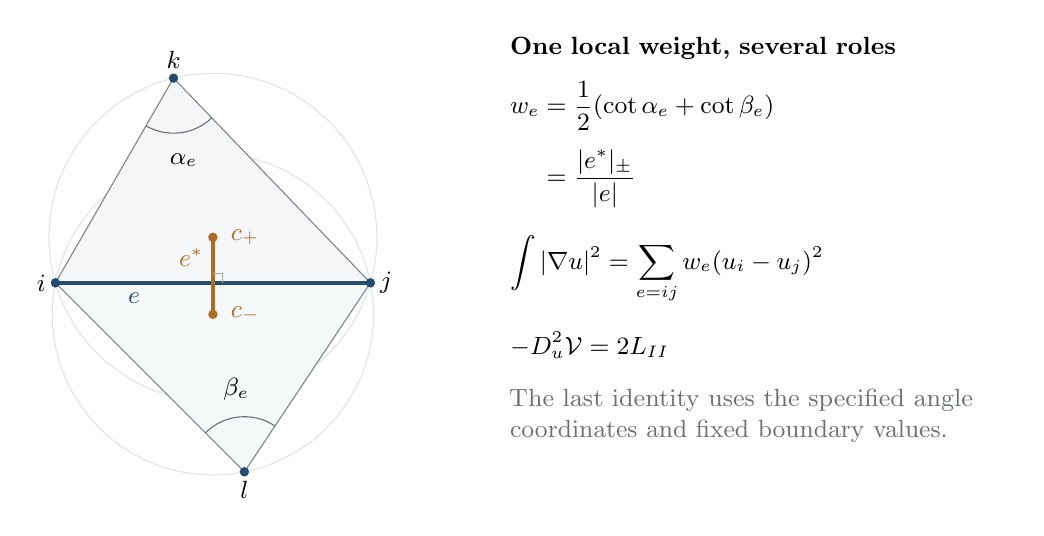
\begin{tikzpicture}[font=\small,line cap=round,>=Latex]
  \begin{scope}[shift={(-5.3,0)}]
    \coordinate (fi) at (0,0); \coordinate (fj) at (4,0);
    \coordinate (fk) at (1.5,2.6); \coordinate (fl) at (2.4,-2.4);
    \coordinate (fc1) at (2,.5788461538); \coordinate (fc2) at (2,-.4);
    \draw[mpblue!15] (fc1) circle (2.082081);\draw[mpblue!15] (fc2) circle (2.039608);
    \fill[mpblue!5] (fi)--(fj)--(fk)--cycle;
    \fill[mpteal!5] (fi)--(fl)--(fj)--cycle;
    \draw[mpgray!85] (fi)--(fk)--(fj) (fi)--(fl)--(fj);
    \draw[mpblue,line width=1.3pt] (fi)--(fj);
    \draw[mpochre,line width=1.7pt] (fc1)--(fc2);
    \draw[mpgray!60] (2.12,0)--(2.12,.12)--(2,.12);
    \pic[draw=mpgray,"$\alpha_e$",angle radius=7mm,angle eccentricity=1.5]
      {angle=fi--fk--fj};
    \pic[draw=mpgray,"$\beta_e$",angle radius=7mm,angle eccentricity=1.5]
      {angle=fj--fl--fi};
    \foreach \p in {fi,fj,fk,fl}\fill[mpblue] (\p) circle (1.7pt);
    \fill[mpochre] (fc1) circle (1.7pt) node[right=3pt] {$c_+$};
    \fill[mpochre] (fc2) circle (1.7pt) node[right=3pt] {$c_-$};
    \node[left] at (fi) {$i$};\node[right] at (fj) {$j$};
    \node[above] at (fk) {$k$};\node[below] at (fl) {$l$};
    \node[below,text=mpblue] at (1,0) {$e$};
    \node[left,text=mpochre] at (2,.32) {$e^*$};
  \end{scope}
  \node[align=left,text width=6.3cm,anchor=west] at (.35,.55) {%
    \textbf{One local weight, several roles}\\[7pt]
    $\displaystyle w_e=\frac12(\cot\alpha_e+\cot\beta_e)$\\[6pt]
    $\displaystyle\hphantom{w_e}=\frac{|e^*|_\pm}{|e|}$\\[9pt]
    $\displaystyle\int |\nabla u|^2=\sum_{e=ij}w_e(u_i-u_j)^2$\\[9pt]
    $\displaystyle -D_u^2\mathcal V=2L_{II}$\\[8pt]
    \textcolor{mpgray}{The last identity uses the specified angle
    coordinates and fixed boundary values.}};
\end{tikzpicture}
\caption[The cotangent Hessian and its finite-element interpretation]{The cotangent weight for two adjacent Euclidean triangles.
The dual segment joins their circumcenters and has signed length
$|e^*|_\pm$; in the locally Delaunay configuration shown, its sign is
positive. The finite-element stiffness matrix is the same cotangent
matrix that appears as minus one half of the volume Hessian in the
coordinates $\alpha_c(u)=\alpha_c^0+u_i-u_j$, with fixed edge-angle
sums and $u=0$ on the boundary. This identity is specific to that
coordinate and constraint system.}
\label{fig:mono-cotangent-hessian}
\end{figure}
% END INLINE FIGURE

\subsection{Boundary response, Schur complements, and a Gaussian factor}
\label{subsec:ipolyResponse}

The subscripts $I$ and $B$ mean interior and boundary vertices;
$L_{IB}$, for example, has interior rows and boundary columns.
A Dirichlet problem fixes boundary voltages and asks for interior
voltages with no injected current. The Neumann data are the currents
needed at the boundary to maintain those voltages.

For a three-vertex path with unit conductances, fix endpoint voltages
$0$ and $1$, and call the middle voltage $x$. The energy is
$x^2+(x-1)^2=2(x-1/2)^2+1/2$. Minimization gives $x=1/2$;
the effective conductance between the endpoints is $1/2$.
Completing this square is the one-variable version of the matrix
elimination below. Integrating $\exp[-(x^2+(x-1)^2)/(2\hbar)]$
over $x$ instead gives $\sqrt{\pi\hbar}\,e^{-1/(4\hbar)}$:
the same effective energy, now with a Gaussian prefactor.

For the finite element network, eliminating the interior voltage gives
\begin{equation}
 v_I=-L_{II}^{-1}L_{IB}v_B,\qquad
 \mathcal N=L_{BB}-L_{BI}L_{II}^{-1}L_{IB}.
 \label{eq:ipolyDtN}
\end{equation}
The matrix $\mathcal N$ maps boundary voltages to boundary currents;
it is the discrete Dirichlet-to-Neumann operator. Indeed, minimizing
$v^TLv$ at fixed $v_B$ gives the first equation and the minimum
$v_B^T\mathcal N v_B$. It follows that $\mathcal N$ is positive
semidefinite and that its kernel consists exactly of boundary constants.
Grounding one boundary vertex, or working modulo constants, makes it
positive definite. This energy statement allows signed boundary weights;
the full passive resistor interpretation requires nonnegative weights.

The same elimination appears in volume response. For a smooth function
with a nondegenerate local maximum at the origin, write
\[
 \mathscr V(x)=V_0-\tfrac12x^TKx+O(|x|^3),\qquad K>0,
\]
and let $Px$ be selected linear observables. These are geometric boundary
data only when the model supplies that identification; they are not the
fixed coordinates $u|_B=0$. The implicit-function theorem gives the local
maximizing branch $x(j)=K^{-1}P^Tj+O(|j|^2)$. Thus perturbation by a
source $j$, or restriction to $Px=b$, gives the local expansions
\begin{align}
 \max_{x\text{ near }0}\{\mathscr V(x)+j^TPx\}
    &=V_0+\tfrac12j^T\chi j+O(|j|^3),
 &\chi&=PK^{-1}P^T,\notag\\
 \max_{\substack{Px=b\\x\text{ near }0}}\mathscr V(x)
    &=V_0-\tfrac12b^T\chi^{-1}b+O(|b|^3),
 \label{eq:ipolyBoundaryResponse}
\end{align}
where the second formula assumes $P$ has full row rank, so $\chi>0$.
The first is the response to a source; the second fixes its conjugate
variable. They are related by a Legendre transform. In the planar
problem $K=2L_{II}$; in the Dehn filling problem, the same algebra gives
\eqref{eq:cuspHessian} and \eqref{eq:cuspmatrixHessian}. This identifies
an exact common operation without identifying their different spaces
of boundary data.

More generally, split $x=(y,z)$ and eliminate $y$. The effective
quadratic form is
\begin{equation}
 K_{\rm eff}=K_{zz}-K_{zy}K_{yy}^{-1}K_{yz},\qquad
 \det K=\det K_{yy}\det K_{\rm eff}.
 \label{eq:ipolySchur}
\end{equation}
For $\hbar>0$, completing the square gives the exact real Gaussian identity
\begin{equation}
 \int_{\mathbb R^{\dim y}}
 e^{-\frac1{2\hbar}(y,z)^TK(y,z)}\,dy
 =\frac{(2\pi\hbar)^{\dim y/2}}{\sqrt{\det K_{yy}}}
       e^{-z^TK_{\rm eff}z/(2\hbar)}.
 \label{eq:ipolyGaussian}
\end{equation}
Thus elimination in the Dirichlet problem, reduction of the classical
boundary action, and its leading Gaussian integration use the same
Schur complement. An oscillatory or complex phase requires the specified
contour and determinant branch, as in the later quantum calculations.
The finite-dimensional identity does not supply those analytic data
or identify an entire quantum invariant by itself.

There is also a combinatorial formula for the planar determinant. Let
$\mathfrak F_B$ be the spanning forests of the weighted graph in which
each component contains exactly one boundary vertex. Then
\begin{equation}
 \boxed{\det(-D_u^2\mathcal V)
      =2^{|I|}\sum_{F\in\mathfrak F_B}\prod_{e\in F}w_e.}
 \label{eq:ipolyForestDeterminant}
\end{equation}
To prove it, write $L_{II}=C_I\operatorname{diag}(w_e)C_I^T$, where
$C_I$ is the incidence matrix with boundary rows removed. Cauchy--Binet
expands its determinant over $|I|$-edge subsets. An incidence minor is
$\pm1$ exactly for a forest rooted at $B$, and zero otherwise. This
rooted-forest formula expresses the local Gaussian determinant in
geometric conductances. It is a deduction from the Hessian identity
and finite-dimensional linear algebra. The incidence-minor identity
holds for real signed weights as well; in the Delaunay Dirichlet problem
its contributing weights are nonnegative. Zero-weight edges contribute
zero terms, and strictness of $L_{II}$ makes the total positive.

\subsection{Why the nonlinear iteration needs a barrier}
\label{subsec:ipolyBarrierComplexity}

A barrier is a function that tends to $+\infty$ at the boundary
of the admissible domain. Minimizing $F-t\mathcal V$ balances
staying safely inside against increasing volume; increasing $t$
gradually reduces the influence of the barrier. A convex function
$f$ is \emph{self-concordant} here if
$|D^3f[h,h,h]|\le2(D^2f[h,h])^{3/2}$ for every direction $h$.
This compares the change of the Hessian with the local scale set
by the Hessian itself, which is what controls Newton steps.
The norm $\|h\|_H=\sqrt{h^THh}$ and its dual
$\|g\|_{H^{-1}}=\sqrt{g^TH^{-1}g}$ will be used below.

A fast linear solve does not by itself bound the number of Newton
steps. In particular, $-\mathcal V$ is not uniformly self-concordant:
near a vanishing angle, its entropy-like behavior makes the normalized
third derivative unbounded. The companion study supplies a more useful
estimate involving the barrier
\begin{equation}
 F(\alpha)=-\sum_c\log\sin\alpha_c.
 \label{eq:ipolyBarrier}
\end{equation}
The coefficient $\csc^2\alpha_c$ occurs in both $D^2F$ and
$D^3\mathcal V$, but these are tensors of different order. The precise
relation needed for optimization is the following inequality.

\begin{proposition}[A barrier compatible with ideal volume]
\label{prop:ipolyCompatibility}
For every positive angle structure and tangent vector $h$ whose
coordinates sum to zero in each triangle,
\begin{equation}
 |D^3\mathcal V[h,h,h]|
 \le\sqrt3\,(-D^2\mathcal V[h,h])\sqrt{D^2F[h,h]}.
 \label{eq:ipolyCompatibility}
\end{equation}
Consequently $F-t\mathcal V$ is self-concordant with the standard
constant for every $t\ge0$. The barrier $F$ has parameter at most
the number $m$ of corner angles.
\end{proposition}

\begin{proof}
For one triangle set $s_i=\sin\alpha_i$ and choose the cyclic side
directions $\psi=(0,\alpha_1+\alpha_2,\pi+\alpha_2)$.
They satisfy $\sum_i s_i e^{i\psi_i}=0$. Every vector with
$h_1+h_2+h_3=0$ can therefore be written
$h_i=\lambda s_i\cos\varphi_i$, where $\varphi_i=\psi_i-\tau$.
The cotangent energy identity and a trigonometric expansion give
\[
 A:=-D^2\mathcal V[h,h]=\lambda^2s_1s_2s_3,\quad
 B:=D^2F[h,h]=\lambda^2\sum_i\cos^2\varphi_i,
\]
\[
 D^3\mathcal V[h,h,h]
   =\lambda^3s_1s_2s_3\cos(\varphi_1+\varphi_2+\varphi_3).
\]
For the last identity, use $\cos^3 x=(3\cos x+\cos3x)/4$ and the
vanishing side-vector sum. Expanding the cosine of the sum shows
$|\cos(\varphi_1+\varphi_2+\varphi_3)|
\le\sum_i|\cos\varphi_i|\le\sqrt{3\sum_i\cos^2\varphi_i}$.
This proves the inequality on one triangle, and summation proves it
globally since $\sum A_T\sqrt{B_T}\le(\sum A_T)\sqrt{\sum B_T}$.
Each $-\log\sin\alpha_c$ is self-concordant, and, with
$A=-tD^2\mathcal V[h,h]$ and $B=D^2F[h,h]$,
\[
 |D^3(F-t\mathcal V)[h,h,h]|
 \le2B^{3/2}+\sqrt3 A\sqrt B\le2(A+B)^{3/2}.
\]
Finally Cauchy--Schwarz gives $|DF[h]|\le\sqrt m\sqrt{D^2F[h,h]}$,
the required barrier-parameter bound. Restriction to additional affine
angle constraints preserves these inequalities.
\end{proof}

All derivatives and inverse local norms in the following argument are
taken on the intrinsic affine angle space, after linear dependencies
have been removed. The parameter bound $m$ belongs to $F$;
$F-t\mathcal V$ is a standard self-concordant objective, not a barrier
claimed to have that same parameter.

Write $\Phi_t=F-t\mathcal V$ and $H_t=D^2\Phi_t$. A nonempty positive
angle domain has compact closure in angle coordinates. Since $F$ tends
to infinity at its relative boundary while $\mathcal V$ is continuous
on the closure, $\Phi_t$ has a unique interior minimizer $x_t$.
The zero-dimensional case is vacuous. If $\mathcal V^*$ denotes the
maximum on the closed feasible domain, then
\[
 \mathcal V^*-\mathcal V(x_t)\le\frac m t.
\]
Indeed, concavity of sine gives
$0\le\sin\beta_c\le\sin x_c+\cos x_c(\beta_c-x_c)$, hence
$DF(x)[\beta-x]\le m$ even for a closed feasible $\beta$ with zero
angles. At $x_t$, use $DF=tD\mathcal V$ and concavity of
$\mathcal V$. This argument does not assume that its closed maximizer
is positive.

For a finite iterate $x$, define the Newton decrement
$\lambda_t(x)=\|D\Phi_t(x)\|_{H_t(x)^{-1}}$. If $\lambda=\lambda_t(x)<1$,
self-concordance gives
$r:=\|x_t-x\|_{H_t(x)}\le\lambda/(1-\lambda)$.
For completeness, put $d=x_t-x$. Along the segment the one-direction
Hessian bound is
$D^2\Phi_t(x+s d)[d,d]\ge r^2/(1+s r)^2$.
Integrating and using stationarity at $x_t$ gives
$-D\Phi_t(x)[d]\ge r^2/(1+r)$, whereas dual Cauchy--Schwarz bounds
the left side by $\lambda r$. Moreover, $H_t\succeq D^2F$ implies
\[
 t\|D\mathcal V(x)\|_{H_t^{-1}}\le\sqrt m+\lambda.
\]
Concavity at $x$ now proves the finite-centering certificate
\[
 \mathcal V^*-\mathcal V(x)
 \le\frac{m+(\sqrt m+\lambda)\lambda/(1-\lambda)}{t}
 \le\frac{17m}{12t}\quad\text{if }\lambda\le\tfrac14,\ m\ge1.
\]

Here is an explicit short-step schedule. Start at $t_0>0$ with
$\lambda_{t_0}(x_0)\le1/4$, increase $t$ by
$1+1/(20\sqrt m)$, and take one full Newton step for the new objective.
With $\delta=(t'-t)/t$, the identities
\[
 D\Phi_{t'}=(1+\delta)D\Phi_t-\delta DF,
 \qquad H_{t'}\succeq H_t
\]
bound the new decrement before the step by
$(1+\delta)/4+\delta\sqrt m\le5/16$.
The standard self-concordant Newton estimate makes the step feasible
and bounds its new decrement by
$(\lambda/(1-\lambda))^2\le25/121<1/4$.
Stopping when $t\ge17m/(12\varepsilon)$ therefore gives
\begin{equation}
 O\!\left(\sqrt m\log\max\left\{e,\frac{m}{t_0\varepsilon}\right\}\right)
 \quad\hbox{Newton steps to volume gap at most }\varepsilon.
 \label{eq:ipolyStepBound}
\end{equation}
This bound assumes the stated initial centering; it does not pay for
finding or centering a feasible point. The underlying Newton estimates
are described in~\cite[Chapter~11]{BoydVandenberghe} and the authors'
lecture notes~\cite{BoydVandenbergheSlides}. They apply here to the
specified barrier schedule, not to unrestricted plain Newton iteration.

In the disk coordinates the Hessian of $F-t\mathcal V$ is again a
grounded planar Laplacian, now with interior conductances
\[
 2t w_e+\csc^2\alpha_e+\csc^2\beta_e.
\]
An energy-norm tolerance makes the inexact version concrete. At the new
parameter, let $d_N=-H^{-1}g$, $\lambda=\|d_N\|_H\le5/16$, and suppose
the computed step satisfies $\|d-d_N\|_H\le\lambda/100$.
Put $\eta=\|d-d_N\|_H$ and $r=\|d\|_H$. Then
$\eta\le1/320$ and $r\le101/320<1$. Hessian comparison and the
integrated gradient remainder give
\[
 \lambda_{\rm new}
 \le\frac{\eta}{1-r}+\frac{r^2}{(1-r)^2}
 \le\frac{10420}{47961}<\frac14.
\]
The old dual-norm linear residual is at most $\eta$, the nonlinear
remainder at most $r^2/(1-r)$, and conversion to the new dual norm
costs at most $1/(1-r)$. This argument assumes exact gradient and
Hessian evaluation apart from the stated solve error. Feasibility can
also be checked directly: $\|d\|_H<1$ and $H\succeq D^2F$ imply
$|d\alpha_c|<\sin\alpha_c\le\min\{\alpha_c,\pi-\alpha_c\}$ for
every corner, so the new angles remain strictly between zero and $\pi$.

Nearly-linear Laplacian solvers provide relative energy-norm
guarantees~\cite[Theorem~5.5]{SpielmanTengSolvers}. With such tolerances
maintained at every step, their combination with
\eqref{eq:ipolyStepBound} gives the conditional randomized expected
$\widetilde O(n^{3/2})$ arithmetic-work scale after centering, up to
accuracy factors. Here $n=|I|+|B|$ is the full mesh vertex count;
disk planarity gives $m=O(n)$ and $O(n)$ matrix entries.
Success probabilities over all solves,
coefficient precision and transcendental evaluations need their own
controls. This is not a bit-complexity or floating-point stability
bound. Finding a feasible point, centering it, and certifying the final
geometric error are separate costs. The companion's selected-input
timings do not bound these additional tasks. The dense implementation
described below follows the specified schedule, with numerical diagnostics;
it does not implement a nearly-linear solver or certify floating-point error.

\subsection{Flips connect the local matrix to mapping-class geometry}
\label{subsec:ipolyFlips}

A diagonal exchange has two different roles. Among triangulations of
the convex hull of a fixed planar vertex set, with fixed nodal values,
Rippa's theorem says that Delaunay
triangulation minimizes the piecewise-linear Dirichlet energy; in matrix
terms $L(\mathcal T_D)\preccurlyeq L(\mathcal T)$~\cite{RippaEnergy}.
This is an ordering of quadratic forms for the same geometric data.
It does not assert monotonicity of hyperbolic volume along an arbitrary
sequence of topological flips.
Figure~\ref{fig:mono-flip} illustrates the comparison for one fixed
Euclidean quadrilateral.

% BEGIN INLINE FIGURE: 08_flip.tex
\begin{figure}[htbp]
\centering
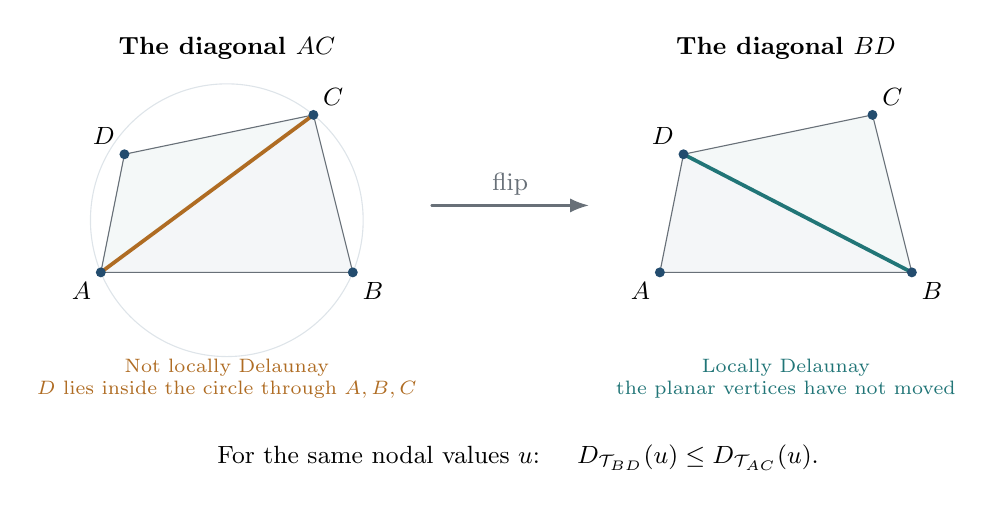
\begin{tikzpicture}[font=\small,>=Latex,line cap=round,line join=round]
  \begin{scope}[shift={(-5.3,0)}]
    \coordinate (fa) at (0,0);\coordinate (fb) at (3.2,0);
    \coordinate (fc) at (2.7,2);\coordinate (fd) at (.3,1.5);
    \draw[mpblue!15] (1.6,.6625) circle (1.731735);
    \fill[mpblue!5] (fa)--(fb)--(fc)--cycle;
    \fill[mpteal!5] (fa)--(fc)--(fd)--cycle;
    \draw[mpgray] (fa)--(fb)--(fc)--(fd)--cycle;
    \draw[mpochre,line width=1.35pt] (fa)--(fc);
    \foreach \p in {fa,fb,fc,fd}\fill[mpblue] (\p) circle (1.8pt);
    \node[below left] at (fa) {$A$};\node[below right] at (fb) {$B$};
    \node[above right] at (fc) {$C$};\node[above left] at (fd) {$D$};
    \node[font=\bfseries\small] at (1.6,2.85) {The diagonal $AC$};
    \node[text=mpochre,align=center,font=\scriptsize] at (1.6,-1.35)
      {Not locally Delaunay\\$D$ lies inside the circle through $A,B,C$};
  \end{scope}
  \draw[->,mpgray,line width=.85pt] (-1.1,.85)--(.9,.85)
    node[midway,above] {flip};
  \begin{scope}[shift={(1.8,0)}]
    \coordinate (ga) at (0,0);\coordinate (gb) at (3.2,0);
    \coordinate (gc) at (2.7,2);\coordinate (gd) at (.3,1.5);
    \fill[mpblue!5] (ga)--(gb)--(gd)--cycle;
    \fill[mpteal!5] (gb)--(gc)--(gd)--cycle;
    \draw[mpgray] (ga)--(gb)--(gc)--(gd)--cycle;
    \draw[mpteal,line width=1.35pt] (gb)--(gd);
    \foreach \p in {ga,gb,gc,gd}\fill[mpblue] (\p) circle (1.8pt);
    \node[below left] at (ga) {$A$};\node[below right] at (gb) {$B$};
    \node[above right] at (gc) {$C$};\node[above left] at (gd) {$D$};
    \node[font=\bfseries\small] at (1.6,2.85) {The diagonal $BD$};
    \node[text=mpteal,align=center,font=\scriptsize] at (1.6,-1.35)
      {Locally Delaunay\\the planar vertices have not moved};
  \end{scope}
  \node[align=center] at (0,-2.35)
    {For the same nodal values $u$: \quad
     $D_{\mathcal T_{BD}}(u)\le D_{\mathcal T_{AC}}(u)$.};
\end{tikzpicture}
\caption[A diagonal exchange and the Delaunay energy comparison]{A diagonal flip on a fixed Euclidean quadrilateral, shown
with its actual vertex positions. Rippa's energy comparison selects the
Delaunay diagonal for fixed nodal values. The same combinatorial move
also occurs in flip graphs used in surface topology; the displayed
energy comparison concerns the fixed Euclidean realization.}
\label{fig:mono-flip}
\end{figure}
% END INLINE FIGURE

For the next comparison, graph distance counts elementary moves.
A \emph{quasi-isometry} preserves large distances up to fixed
multiplicative and additive errors, with every target point within
a bounded distance of its image. It does not identify individual
edge lengths or local metrics. A mapping torus is formed from
$S\times[0,1]$ by identifying $(x,1)$ with $(f(x),0)$ for a surface
map $f$; its monodromy is the mapping class of $f$.
Pseudo-Anosov classes are those with the invariant stretching and
contracting measured foliations used in surface dynamics. The
comparison theorems below are external inputs, with their surface
and boundary hypotheses retained.

For a connected orientable finite-type marked surface admitting an ideal
triangulation, with at least one marked point on every boundary curve,
the graph of ideal triangulations and diagonal exchanges is instead
a coarse geometric model of its mapping class group. For orientation-
preserving classes and isotopies fixing the marked points individually,
the action is proper and cocompact, and an
orbit map is a quasi-isometry~\cite[Section~2.1, Lemma~2.3]{DisarloParlier}.
For a closed oriented surface of genus at least two, the pants graph is
a different model, quasi-isometric to Teichm\"uller space with its WP
metric. In this setting Brock compares the convex-core volume of the
quasi-Fuchsian manifold with conformal ends $X,Y$ to $d_{\rm WP}(X,Y)$,
with topology-dependent multiplicative and additive
constants~\cite[Theorems~1.1--1.2]{BrockWPVolumes}.
For pseudo-Anosov monodromy on the same closed surface, mapping-torus
volume and WP translation distance are comparable with topology-dependent
multiplicative constants~\cite[Theorem~1.1]{BrockMappingTori}.
The flip graph and pants graph have different metric roles.

There is a direct volume estimate when a flip sequence gives a layered
ideal triangulation of a hyperbolic mapping torus with $N$ tetrahedra:
straightening gives $\operatorname{Vol}(M)\le Nv_3$, where $v_3$ is the
volume of the regular ideal tetrahedron. This does not require the
given triangulation to have positive geometric shapes; signed
straightened volumes still have absolute value at most $v_3$.
It connects a combinatorial decomposition length to three-dimensional
volume. Comparing it further to WP geometry requires a theorem for the
same surface and boundary conventions, rather than transferring the
closed-surface theorem silently to a punctured surface.

\subsection{The three-manifold extension and the remaining questions}
\label{subsec:ipolyThreeManifolds}

The Casson--Rivin program uses the same ideal-tetrahedron volume and the
same angle-sum constraints~\cite{FuterGueritaud}. Its local Hessian is
still a cotangent quadratic form. For leading--trailing edge variables
$y_e$, put $p_\alpha=y_e+y_{e'}$ for the pair of opposite tetrahedron
edges carrying $\alpha$, and cyclically for $\beta,\gamma$. Then
\begin{equation}
 -D^2\mathcal V
 =\sum_t\left[
 \cot\alpha_t(dp_\gamma-dp_\beta)^2
 +\cot\beta_t(dp_\alpha-dp_\gamma)^2
 +\cot\gamma_t(dp_\beta-dp_\alpha)^2\right].
 \label{eq:ipolyThreeDimensionalHessian}
\end{equation}
This displays the Euclidean cusp-link triangle inside the second
variation. But a square now involves sums of opposite-edge variables,
and the assembled matrix need not have nonpositive off-diagonal entries
or be diagonally dominant. Additional peripheral directions and removal
of linear dependencies must also be included in a full coordinate
system. The planar positive-Laplacian solver conclusion therefore does
not transfer automatically to arbitrary three-manifold triangulations.
The trianglewise barrier estimate does transfer, because it survives
affine restriction.

For an ideal triangulation of an orientable compact three-manifold whose
nonempty boundary is a union of tori, a positive angle structure critical
for volume on the full angle space supplies the complete hyperbolic
metric on its interior, by the Casson--Rivin
theorem~\cite[Theorem~1.2]{FuterGueritaud}. The angle space has triangle
sums $\pi$ and edge sums $2\pi$; full criticality includes the peripheral
directions. Edge variations alone do not impose completeness.
A boundary maximizer need not realize the
chosen triangulation by positive ideal tetrahedra. Optimization on a
given angle polytope therefore does not solve the problem of finding
a suitable geometric triangulation or yield a polynomial-time
geometrization algorithm.

The finite element comparison also does not identify its real symmetric
Hessian with the alternating WP form. The exact links established here
are the volume Hessian, its inverse response, its Schur complement,
and its Gaussian determinant. A continuum limit relating appropriately
renormalized polyhedral functionals to a WP potential would require
geometric convergence, a specified normalization, and control of second
variations. This is a natural question, not a theorem asserted here.
Likewise, in three dimensions it remains useful to ask for an effective
bound on the smallest angle at an interior maximum in terms of the
number of tetrahedra and a quantitative feasible margin. Such a bound
would connect variational existence to numerical certification and
complexity. These questions describe how the computational strand can
extend the monograph's variational and semiclassical program.

\subsection{Reproducible computational examples}
\label{subsec:ipolyComputation}

The \href{../experiments/section9/README.md}{Section 9 reproduction guide}
connects these formulas to a fixed $3$ by $2$ integer-coordinate grid,
triangulated into twelve right-isosceles triangles with two interior
vertices. At its geometric angle assignment,
\[
 L_{II}=\begin{pmatrix}4&-1\\-1&4\end{pmatrix},\qquad
 K=-D_u^2\mathcal V=\begin{pmatrix}8&-2\\-2&8\end{pmatrix},\qquad
 \det K=60.
\]
An independent rational finite-element assembly gives this matrix.
Exhaustive boundary-rooted forest enumeration gives fifteen unit-weight
terms, so \eqref{eq:ipolyForestDeterminant} gives $2^2\cdot15=60$.
Eliminating the first variable of $K$ leaves $K_{\rm eff}=15/2$, and
$8(15/2)=60$. Prescribing the electrical boundary voltage $v=x/3$
gives interior values $1/3,2/3$ and energy $2/3$. These are exact finite
identities for the named fixture, separate from the general proofs above.

The \href{../packages/volume-toolkit/ideal_poly_volume_toolkit/variational.py}
{maintained numerical operators} assemble angle increments, gradients,
Hessians and boundary response. The
\href{../experiments/section9/run.py}{experiment driver} also compares
the binary64 volume with $12G$, where $G$ is Catalan's constant, and an
off-origin Hessian with independent numerical differentiation at 50-digit
working precision. The \href{../artifacts/section9/result.json}{result record}
states source and input hashes, methods, residuals and tolerances.
These numerical comparisons are not interval enclosures.

The \href{../site/section9/index.html}{worked computational companion}
and \href{../site/section9/downloads/section9-reproduction.zip}{complete
reproduction archive} provide the input, runnable code and environment
requirements. The grid has zero-weight square diagonals and is therefore
non-strict Delaunay. Off-origin angles belong to the abstract domain;
their geometric closure is not asserted.

The separate \href{../site/section9/barrier.html}{barrier examples} exercise
the \href{../packages/volume-toolkit/ideal_poly_volume_toolkit/angle_barrier.py}
{dense affine-angle solver}. It accepts a supplied positive angle vector
and independent tangent columns, performs separately budgeted initial
centering, and then follows the short-step parameter schedule above.
Every accepted point records its parameter, Newton decrement, angle margins,
linear-solve residual and numerical conditioning. Rejected domains, failed
steps and exhausted budgets remain unsuccessful outcomes; angles are not
clipped into the domain. The reported finite-gap estimate is evaluated in
binary64 arithmetic and is not an interval certificate.

The \href{../experiments/section9/barrier_run.py}{barrier experiment driver}
compares the computed endpoints with independent multiprecision volume
references and checks the recorded path and stopping conditions. The fixed
cases are the full single-triangle angle simplex with its maximum at the
regular ideal tetrahedron, an asymmetric rectangular disk, and a two-triangle
affine slice with one flat triangle at its closed maximum. Its
\href{../artifacts/section9/barrier-result.json}{result record} separates
initial-centering work from path steps, and its
\href{../site/section9/downloads/barrier-reproduction.zip}{reproduction archive}
contains the actual code, inputs and environment requirements. These finite
examples do not establish a scaling law. A nearly-linear solver, a certified
relative energy-error bound, a peripheral-holonomy solver and a global
realization certificate remain outside this implementation. The
\href{claims/section9.json}{claim ledger} distinguishes this numerical
coverage from the general proofs, external theorem inputs and open questions.


\monographpart{Quantum geometry, degeneration, and surgery}{An introduction to the quantum constructions leads to exact period comparisons, a controlled tetrahedral degeneration, and the classical and Gaussian data of Dehn filling.}

\section{A geometric introduction to the quantum constructions}
\label{sec:quantumintro}

The next part uses several constructions that share the word
\emph{quantum} but have different definitions. This section introduces
the objects, the elementary asymptotic mechanism, and the distinctions
needed to read the calculations. The prerequisites are representation
theory at the level of tensor products, elementary complex analysis,
and the geometry already discussed. No physical interpretation is
needed for the finite sums or special-function identities.

The organizing operation is cutting and gluing. A decomposition gives
intermediate labels; changing the decomposition gives a change-of-basis
matrix or integral kernel. The quantum constructions make these
operations exact. In suitable large-parameter limits their equations
recover geometric gluing, and their leading exponents recover geometric
actions. The simplest complete example below is a finite sum for the
figure-eight knot whose growth gives the volume of two regular ideal
tetrahedra.

\subsection{Six labels: recoupling and tetrahedral weights}
\label{sec:introrecoupling}

Let $V_j$ be the irreducible $\mathfrak{sl}_2$-representation of dimension
$2j+1$, where $j$ is a nonnegative half-integer. Consider
\[
 \operatorname{Hom}_{\mathfrak{sl}_2}(V_d,V_a\otimes V_b\otimes V_c).
\]
There are two natural bases. One first decomposes $V_a\otimes V_b$
and records an intermediate representation $V_s$; the other first
decomposes $V_b\otimes V_c$ and records $V_t$. Thus
\begin{equation}
 B_s^{(ab)c}=\sum_t F_{st}^{abc;d}B_t^{a(bc)}.
 \label{eq:introrecoupling}
\end{equation}
The coefficients depend on six labels $a,b,c,d,s,t$. With conventional
dimension and sign factors, they are the \emph{$6j$-symbols}. The
four admissible triples
\[
 (a,b,s),\quad(s,c,d),\quad(b,c,t),\quad(a,t,d)
\]
can be assigned to the four faces of a tetrahedron. At this point the
tetrahedron is a way to organize the labels. Its interpretation as a
metric tetrahedron requires an additional asymptotic statement.

A quantum group deforms this tensor-product calculus. For
$U_{q_{\rm alg}}(\mathfrak{sl}_2)$, ordinary integers and factorials in
the explicit formulas are replaced by their quantum analogues, for example
\begin{equation}
 [n]_{q_{\rm alg}}
 =\frac{q_{\rm alg}^{n}-q_{\rm alg}^{-n}}
        {q_{\rm alg}-q_{\rm alg}^{-1}},\qquad
 [n]_{q_{\rm alg}}\longrightarrow n\quad(q_{\rm alg}\to1).
 \label{eq:introqinteger}
\end{equation}
The full definition also specifies tensor products and braidings; it
is not merely a rule for replacing integers. At the usual compact
root $q_{\rm alg}=e^{\pi i/r}$, the finite fusion theory retains the
labels $0,\frac12,\ldots,\frac{r-2}{2}$. A triple must satisfy the
triangle inequalities, integral total spin, and
$a+b+c\le r-2$. Taylor--Woodward give the representation-theoretic
definition and these conventions explicitly~\cite{TaylorWoodward}.

Associating four tensor factors in the five possible ways gives the
\emph{pentagon identity}. In tetrahedral language it supplies the
identity for replacing two tetrahedra by three in a triangulated ball.
Together with orthogonality and normalization identities, this makes
state sums independent of the triangulation. Schematically, a
Turaev--Viro sum for a closed triangulated manifold has the form
\begin{equation}
 Z_r(M)=C_r(T)\sum_{\text{admissible edge labels }\mathbf j}
       \prod_{e\in E(T)}d_{j_e}\,
       \prod_{\Delta\in T}\{6j\}_{\Delta,\mathbf j}.
 \label{eq:introstatesum}
\end{equation}
Here $T$ is a triangulation, $d_j$ is a quantum dimension, and $C_r(T)$
is the prescribed normalization. This displayed formula explains the
structure; the exact weights are part of the definition of the chosen
theory~\cite[Sections 2.2--2.3]{ChenYang}. A \emph{state} in this sum
is an admissible assignment of labels. The sum is over such assignments;
a description as an integral over hyperbolic metrics, with a particular
geometric measure, would be a further result.

\subsection{The invariants and their volume limits}
\label{sec:introinvariants}

The main objects used below can be distinguished by their inputs and
outputs.
\begin{center}
\small
\begin{tabular}{@{}>{\raggedright\arraybackslash}p{0.23\textwidth}>{\raggedright\arraybackslash}p{0.32\textwidth}>{\raggedright\arraybackslash}p{0.39\textwidth}@{}}
\toprule
Object & Input & Output and construction\\
\midrule
Colored Jones $J_N$ & Knot, color $N$, variable $q_J$
& A Laurent polynomial, from braid or skein calculus.\\[4pt]
Kashaev invariant & Knot and integer $N$
& The specialization $J_N(K;e^{2\pi i/N})$ in the reduced convention.\\[4pt]
Reshetikhin--Turaev (RT) & Closed oriented three-manifold and root/level
& A scalar, from weighted colored-link evaluations of a surgery presentation.\\[4pt]
Turaev--Viro (TV) & Closed three-manifold and root/level
& A scalar state sum, built from tetrahedral $6j$-weights.\\[4pt]
Continuous $b$-$6j$ & Six continuous representation parameters and $b$
& A change-of-basis kernel for a noncompact representation theory.\\[4pt]
Liouville correlation & Marked conformal surface, insertion parameters, and $b$
& A function of the marked points, obtained by averaging field insertions.\\
\bottomrule
\end{tabular}
\end{center}
The first four objects are topological invariants with their prescribed
normalizations. The last two supply analytic kernels and functions
that enter the comparisons in this monograph. In particular, a local
$6j$-weight is not already a three-manifold invariant.

The knot construction begins with a braid whose closure is the knot.
A crossing acts by a braiding matrix on the tensor product of the
strand representations; the Yang--Baxter equation gives the braid
relation. A quantum trace, adjusted to the representation theory,
closes the strands, and the prescribed normalization handles the
moves that change the braid presentation~\cite[Section 2]{MurakamiIntro}.

For the colored Jones polynomial, the color $N$ denotes the
$N$-dimensional representation at generic parameter. We use the
\emph{reduced} normalization $J_N(\text{unknot};q_J)=1$, and specialize
only after forming that polynomial. Murakami--Murakami identify this
specialization with Kashaev's invariant~\cite{MurakamiMurakami}.
For a hyperbolic knot, the volume conjecture is
\begin{equation}
 \lim_{N\to\infty}\frac{2\pi}{N}
 \log|J_N(K;e^{2\pi i/N})|=\Vol(S^3\setminus K).
 \label{eq:introknotvolume}
\end{equation}
The right side is the ordinary three-dimensional hyperbolic volume,
not a volume of moduli space. The assertion concerns a sequence in
which both the color and the root change.

The closed-manifold version used in Section~\ref{sec:dehnresponse}
is the Chen--Yang asymptotic at their root $\zeta_r=e^{2\pi i/r}$,
with $r$ odd:
\begin{equation}
 \frac{4\pi}{r}\log|\mathrm{RT}_r(M;\zeta_r)|\longrightarrow\Vol(M),
 \qquad
 \frac{2\pi}{r}\log\mathrm{TV}_r(M;\zeta_r)\longrightarrow\Vol(M).
 \label{eq:introclosedvolume}
\end{equation}
These statements are conjectural in general, with theorems for
specified families; the hyperbolic fillings of the figure-eight used
later are covered by Wong--Yang~\cite{WongYangDehn}. The doubling
relation between matching RT and TV theories explains the factor
two between their leading logarithms. Exact identities require
consistent choices: generally $\mathrm{TV}_{\mathcal C}$ is the RT
invariant of the categorical center, and the familiar modulus-square
formula holds in the matching unitary modular setting
\cite{TuraevVirelizier}. One should not equate differently normalized
$\mathrm{SU}(2)$ and $\mathrm{SO}(3)$ versions without conversion.

There are two root-of-unity subtleties. First, authors use parameters
differing by a square: in a common convention $q_J=q_{\rm alg}^2$.
Within Chen--Yang's conventions, the volume root $e^{2\pi i/r}$
differs from the standard compact root $e^{\pi i/r}$; the latter
belongs to a different asymptotic problem~\cite{ChenYang}.
Second, even where the numerical roots agree after changing notation,
the colors may not belong to the same theory. At
$q_{\rm alg}=e^{\pi i/N}$, the $N$-dimensional color has
$[N]_{q_{\rm alg}}=0$ and lies outside the retained simple labels
of the level-$N-2$ compact fusion theory. Reducing $J_N$ first and
then specializing is essential. Thus the Kashaev limit should not
be read as an allowed fixed-color observable in that finite unitary
theory.

\subsection{A complete example: the figure-eight knot}
\label{sec:introfigureeight}

For the figure-eight knot $4_1$, the root specialization is an
especially simple positive sum:
\begin{equation}
 \boxed{\quad
 J_N(4_1;e^{2\pi i/N})=\sum_{k=0}^{N-1}P_{N,k},\qquad
 P_{N,k}=\prod_{j=1}^{k}4\sin^2\frac{\pi j}{N},\quad P_{N,0}=1.
 \quad}
 \label{eq:introfigureproduct}
\end{equation}
Kashaev gives the product formula~\cite[eqs. (2.2), (2.5)]{KashaevVolume}.
The following elementary asymptotic proof is presented by
Murakami and credited there to Ekholm~\cite[Section 3.2]{MurakamiIntro}.

The ratio of consecutive products is
\[
 \frac{P_{N,k}}{P_{N,k-1}}=4\sin^2\frac{\pi k}{N}.
\]
It is less than one before $N/6$, greater than one between $N/6$
and $5N/6$, and less than one afterward. The global maximum is
therefore attained at $m_N=\lfloor5N/6\rfloor$, allowing an adjacent
tie. To compare with the initial value $1$, use the elementary
identity $P_{N,N-1}=N^2$. Positivity now gives
\[
 P_{N,m_N}\le J_N(4_1;e^{2\pi i/N})\le N P_{N,m_N}.
\]
The two logarithmic bounds differ by $\log N$, which disappears
after division by $N$. The remaining Riemann sum has an integrable
logarithmic singularity at zero, and yields
\begin{equation}
 \lim_{N\to\infty}\frac1N\log J_N(4_1;e^{2\pi i/N})
 =\int_0^{5/6}\log(4\sin^2\pi x)\,\dd x.
 \label{eq:introfigureintegral}
\end{equation}
The endpoint causes no difficulty: subtract $2\log x$ near zero;
the remaining function is continuous and the logarithmic part is
controlled by Stirling's formula.

Define the Lobachevsky function by
\[
 \Lambda(\theta)=-\int_0^\theta\log|2\sin t|\,\dd t.
\]
Its elementary symmetry and duplication identities give
\begin{align}
 \lim_{N\to\infty}\frac{2\pi}{N}
       \log J_N(4_1;e^{2\pi i/N})
 &=-4\Lambda(5\pi/6)=4\Lambda(\pi/6)\notag\\
 &=6\Lambda(\pi/3)=2v_3
  =\Vol(S^3\setminus4_1),
 \label{eq:introfigurevolume}
\end{align}
where $v_3=3\Lambda(\pi/3)$ is the volume of a regular ideal
tetrahedron. The complete figure-eight complement consists of two
such tetrahedra. Its volume is approximately $2.02988321$.

This calculation already displays the mechanism: an exact quantum
sum, a logarithmic classical phase, a dominant critical point,
and a geometric critical value. It also shows why selecting the
critical point matters. For
$f(t)=\int_0^t\log(4\sin^2\pi x)\,\dd x$, the stationary point
$t=1/6$ is a minimum, while $t=5/6$ is the relevant maximum.
Here positivity controls the entire sum. Complex-valued sums and
integrals require a separate analysis of their contributing
critical points and possible cancellation.

\subsection{Why dilogarithms occur}
\label{sec:introdilog}

An elementary convergent product explains the terminology. For
$\varepsilon>0$ and $|z|<1$, set
\[
 (z;e^{-\varepsilon})_\infty
      =\prod_{n=0}^\infty(1-ze^{-n\varepsilon}).
\]
Expanding the logarithm and summing the geometric progression gives
\begin{align}
 \log(z;e^{-\varepsilon})_\infty
 &=-\sum_{m=1}^\infty
       \frac{z^m}{m(1-e^{-m\varepsilon})}\notag\\
 &=-\frac{\operatorname{Li}_2(z)}{\varepsilon}
       +\frac12\log(1-z)+O(\varepsilon),
 \label{eq:introqpochhammer}
\end{align}
uniformly on compact subsets of $|z|<1$.
The logarithm of this ``quantum dilogarithm'' has the ordinary
dilogarithm as its leading term. Faddeev--Kashaev's quantum
pentagon identity deforms the classical five-term dilogarithm
identity~\cite{FaddeevKashaev}.

The geometry enters in two ways. For an oriented ideal tetrahedron
with shape $z$ in the upper half-plane,
\begin{equation}
 \Vol(T_z)=D(z)
 =\Im\operatorname{Li}_2(z)+\arg(1-z)\log|z|.
 \label{eq:introBlochWigner}
\end{equation}
The logarithmic correction matters: an arbitrary dilogarithm phase
does not have volume as its imaginary part without the appropriate
boundary terms. Also,
$\dd\operatorname{Li}_2(z)=-\log(1-z)\,\dd\log z$.
Consequently differentiation of a sum of dilogarithms produces
logarithms of tetrahedral shapes, which can impose gluing equations.

Here is a particularly direct version in the convention of
Dimofte--Garoufalidis~\cite[Section 5.1]{DimofteGaroufalidis}.
Their tetrahedral quantum function obeys
\begin{equation}
 \psi_\hbar(Z+\hbar)=(1-e^{-Z})\psi_\hbar(Z),\qquad
 \log\psi_\hbar(Z)\sim\frac1\hbar\operatorname{Li}_2(e^{-Z})+O(1).
 \label{eq:introquantumshape}
\end{equation}
Putting $\psi_\hbar\sim e^{S/\hbar}$ in the difference equation
gives $e^{S'(Z)}=1-e^{-Z}$. With $z=e^Z$, the right side is
the companion tetrahedral shape $1-z^{-1}$. Thus a difference
equation for a special function becomes an algebraic shape relation
in the limit.

A \emph{state integral} combines these tetrahedral functions with
quadratic exponential factors determined by the gluing data and
integrates over internal logarithmic variables. Differentiating its
leading phase gives the logarithmic gluing equations; exponentiating
them gives the familiar products of shapes around edges. The
boundary variables are retained as arguments of the integral.
The precise quadratic term, logarithm branches, and contour are
part of the construction. The convergent product in
\eqref{eq:introqpochhammer} explains the mechanism in a simple
domain; one cannot substitute a unit-modulus root into that product
and assume it converges. The continued or noncompact functions used
later have their own definitions and contour prescriptions.
\subsection{Stationary phase, loops, torsion, and degenerate saddles}
\label{sec:introsemiclassical}

The word \emph{semiclassical} means an asymptotic regime in which
the quantum parameter tends to zero while the intended geometric
data remain controlled. Much of the calculation is ordinary
asymptotic analysis. Consider
\begin{equation}
 I(\hbar)=\int_\Gamma e^{S(x)/\hbar}
                 a(x;\hbar)\,\dd^m x,
 \qquad a(x;\hbar)=a_0(x)+\hbar a_1(x)+\cdots.
 \label{eq:introsaddleintegral}
\end{equation}
Suppose $x_*$ is a nondegenerate critical point with $a_0(x_*)\ne0$,
the parameter tends
to zero along a fixed ray, and $\Gamma$ contains the corresponding
steepest-descent cycle. Taylor expansion and Gaussian integration
give its local contribution
\begin{equation}
 I_{x_*}(\hbar)\sim
 e^{S(x_*)/\hbar}(2\pi\hbar)^{m/2}
 \frac{a_0(x_*)}{\sqrt{\det(-S''(x_*))}}
 (1+c_1\hbar+\cdots).
 \label{eq:introgaussian}
\end{equation}
The contour fixes the phase and square-root branch. For a real
Laplace integral with a strict maximum this is the usual Gaussian
formula; for a complex phase it is applied along suitable real
$m$-dimensional contours in the complexified variables.

This formula gives a useful translation of the physics terminology.
The \emph{classical} or \emph{tree-level} contribution is the
critical value $S(x_*)/\hbar$. The \emph{one-loop} contribution
includes the Gaussian determinant and leading amplitude or measure
factors. Higher-loop terms come from the higher Taylor derivatives
and amplitude corrections. Feynman diagrams organize the Gaussian
contractions needed to compute these coefficients; the terminology
does not require an additional physical assumption. In logarithmic
form one writes
\[
 \log I_{x_*}=\frac{S_0}{\hbar}
      +\nu\log\hbar+S_1+S_2\hbar+\cdots,
\]
where $\nu$ depends on the integral's normalization and any zero
modes (kernel directions of the linearized operator). A geometric expansion of $S_0$ in a shrinking area or an
inverse Dehn-filling slope is a separate expansion. The cubic and
quintic Neumann--Zagier coefficients are not, on that account,
quantum higher-loop coefficients.

\emph{Torsion} is the topological form taken by a determinant of
linearized equations after gauge directions have been accounted
for. For a flat holonomy representation $\rho$, the relevant
cellular complex is $C^\bullet(M;\operatorname{Ad}\rho)$, with the
holonomy acting on the Lie algebra by conjugation.
Its $H^0$ records infinitesimal stabilizers and its $H^1$ records
infinitesimal deformations. Reidemeister torsion compares the
specified cellular bases with bases adapted to the differentials,
using an alternating product of determinants. Nonzero cohomology
requires cohomology bases as well; for a cusped three-manifold,
peripheral curves enter this normalization. This explains the
appearance of adjoint torsion in semiclassical amplitudes
\cite{WittenJones,DimofteGaroufalidis}.

An individual Hessian determinant is not the torsion by definition:
measure factors, gauge directions, and basis conventions must be
matched. In the surgery convention used below the relevant
amplitude is proportional to $\operatorname{Tor}^{-1/2}$.
Section~\ref{sec:dehnresponse} supplies the actual peripheral and
solid-torus factors and an established figure-eight comparison.

There is also a global question. A \emph{Lefschetz thimble} is a
steepest-descent cycle attached to a critical point. Under the
usual analytic hypotheses, the exact contour can be represented
in an appropriate relative homology group as
\[
 \Gamma=\sum_\alpha n_\alpha\mathcal J_\alpha.
\]
The coefficients determine which saddles contribute. Their
description can change across a \emph{Stokes locus} as parameters
vary; the exact integral can remain analytic while its decomposition
into saddle contributions changes~\cite[Sections 2--3]{WittenContinuation}.
To recover the asymptotic of a whole invariant, one must control
these coefficients, all competing contributions, and cancellation.
The figure-eight positive sum supplied this global control by an
elementary inequality. A local geometric saddle in a general
state integral supplies only its local contribution until these
additional questions are settled.

Finally, a degenerate Hessian changes the local model. At a simple
fold, two saddles merge. After separating the nondegenerate
transverse directions, the remaining phase has the form
\[
 S(x;t)=S_0+\frac{x^3}{3}-tx+\text{higher terms}.
\]
The substitution $x=\hbar^{1/3}y$, $t=\hbar^{2/3}s$ gives
\[
 \frac{S-S_0}{\hbar}=\frac{y^3}{3}-sy+\cdots.
\]
The resulting contour integral is an Airy integral, rather than
a sum of two separately uniform Gaussian approximations. This
explains the exponent $2/3$ in the transition scale. For the regular
family in Section~\ref{sec:quantumAiry}, the real small parameter
is $h=2\pi b^2$, so the geometric deformation has scale
$b^{4/3}$. When that deformation is proportional to boundary area
$A$, the same scale follows from $W\asymp A^{3/2}$ and $W/h=O(1)$.
The later theorem proves the necessary contour and error estimates
for its specified family; the scaling argument alone does not.


% BEGIN INLINE FIGURE: 09_airy.tex
\begin{figure}[htbp]
\centering
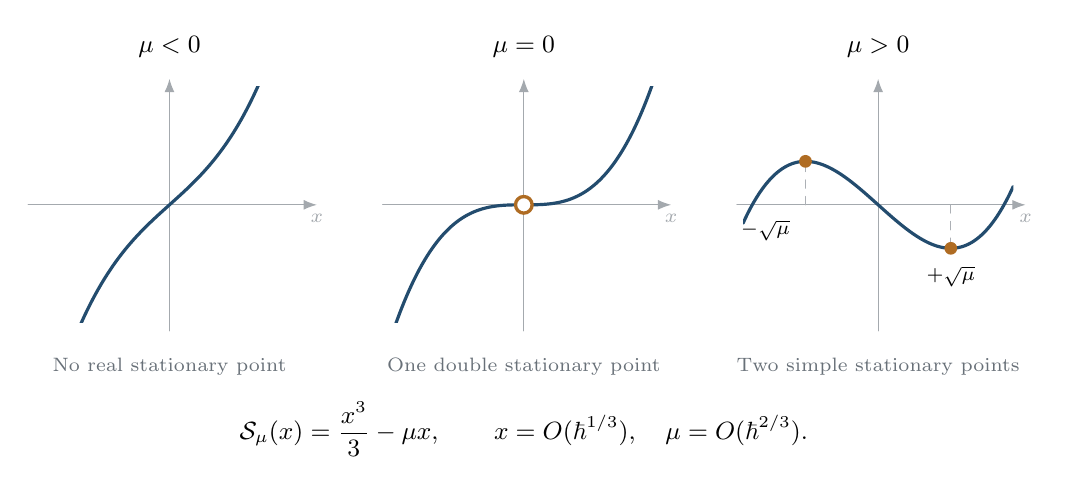
\begin{tikzpicture}[font=\small,>=Latex,line cap=round]
  \foreach \shift/\mval/\heading in {-4.5/-1.4/{$\mu<0$},0/0/{$\mu=0$},4.5/1.4/{$\mu>0$}} {
    \begin{scope}[shift={(\shift,0)}]
      \node[font=\bfseries\small] at (0,2.0) {\heading};
      \begin{scope}[x=.78cm,y=.5cm]
        \draw[->,mpgray!60] (-2.3,0)--(2.4,0) node[below,font=\scriptsize] {$x$};
        \draw[->,mpgray!60] (0,-3.2)--(0,3.2);
        \begin{scope}
          \clip (-2.2,-3) rectangle (2.2,3);
          \draw[mpblue,line width=1.15pt,domain=-2.2:2.2,samples=150]
            plot (\x,{\x*\x*\x/3-\mval*\x});
        \end{scope}
      \end{scope}
    \end{scope}
  }
  \filldraw[draw=mpochre,fill=white,line width=1.2pt] (0,0) circle (3pt);
  \begin{scope}[shift={(4.5,0)},x=.78cm,y=.5cm]
    \draw[mpgray!55,dashed] (-1.183216,0)--(-1.183216,1.104334)
      (1.183216,0)--(1.183216,-1.104334);
    \fill[mpochre] (-1.183216,1.104334) circle (2.3pt);
    \fill[mpochre] (1.183216,-1.104334) circle (2.3pt);
    \node[below left=3pt,font=\scriptsize] at (-1.183216,0) {$-\sqrt\mu$};
    \node[below=3pt,font=\scriptsize] at (1.183216,-1.104334) {$+\sqrt\mu$};
  \end{scope}
  \node[align=center,text=mpgray,font=\scriptsize] at (-4.5,-2.05) {No real stationary point};
  \node[align=center,text=mpgray,font=\scriptsize] at (0,-2.05) {One double stationary point};
  \node[align=center,text=mpgray,font=\scriptsize] at (4.5,-2.05) {Two simple stationary points};
  \node[align=center] at (0,-2.85)
    {$\mathcal S_\mu(x)=\displaystyle\frac{x^3}{3}-\mu x,
      \qquad x=O(\hbar^{1/3}),\quad \mu=O(\hbar^{2/3})$.};
\end{tikzpicture}
\caption[Coalescing stationary points and the Airy normal form]{The cubic normal form for an Airy transition. The stationary
equation is $x^2=\mu$; two stationary points merge at $\mu=0$.
The scaling shown balances the cubic and linear terms in
$\exp(i\mathcal S_\mu/\hbar)$. This is a normal-form illustration,
not the full phase or integration contour of a quantum invariant;
normalization, amplitudes, and contour tails require the separate
estimates in the text.}
\label{fig:mono-airy}
\end{figure}
% END INLINE FIGURE

\subsection{Flat connections, Chern--Simons theory, and boundary states}
\label{sec:introCS}

The connection with hyperbolic geometry can be phrased using flat
connections. If $\mathscr A$ is a connection one-form, its curvature
is $F_{\mathscr A}=\dd\mathscr A+\mathscr A\wedge\mathscr A$.
In a chosen trivialization the Chern--Simons functional has the form
\begin{equation}
 \operatorname{CS}(\mathscr A)=\frac1{4\pi}\int_M
   \tr\left(\mathscr A\wedge\dd\mathscr A
                    +\frac23\mathscr A\wedge\mathscr A\wedge\mathscr A\right).
 \label{eq:introCSfunctional}
\end{equation}
The trace convention fixes the periods and overall normalization.
On a closed manifold its first variation is
$\delta\operatorname{CS}=(2\pi)^{-1}\int_M
\tr(\delta\mathscr A\wedge F_{\mathscr A})$.
Thus the critical points are flat connections modulo gauge.
The formal expression
$\int e^{ik\operatorname{CS}(\mathscr A)}\,D\mathscr A$
motivates the theory; exact algebraic constructions of quantum
invariants do not depend on treating this symbol as an ordinary
convergent integral~\cite{WittenJones}.

For the compact group $\mathrm{SU}(2)$, the flat connections form
the compact character-variety problem. Hyperbolic three-dimensional
holonomy instead takes values in $\mathrm{PSL}_2(\CC)$, with a lift
to $\mathrm{SL}_2(\CC)$ when chosen. It supplies a distinguished
\emph{complex} flat connection. The correctly normalized complex
Chern--Simons action contains both the volume and the Chern--Simons
invariant. Analytic continuation and the choice of integration
cycle connect these settings; merely changing the name of the
gauge group does not specify the cycle~\cite{GukovApoly,WittenContinuation}.

For a manifold with boundary, variation of the functional has a
boundary term. This is the source of the symplectic form on boundary
flat connections and the need to specify boundary data. Abstractly,
a topological quantum field theory assigns a vector space
$\mathcal H(\Sigma)$ to an oriented surface, and a vector
$\Psi_M\in\mathcal H(\partial M)$ to a three-manifold with boundary.
Gluing is a pairing:
\[
 Z(M_1\cup_\Sigma M_2)=\langle\Psi_{M_1},\Psi_{M_2}\rangle,
\]
with orientation reversal supplying the dual space and the theory's
framing conventions understood. In finite root-of-unity theories
this is finite-dimensional linear algebra. In the analytic models
used for complex holonomy, a state is represented locally by a
function or distribution of continuous boundary variables, and
the pairing becomes an integral. Those analytic models require
their own existence and convergence statements.

A \emph{polarization} chooses which half of the conjugate boundary
coordinates are arguments of the state. For a torus boundary,
use the multiplier logarithms $u,v$ of Section~\ref{sec:dehnresponse}.
The Neumann--Zagier normalization is
\begin{equation}
 \Omega_\partial=\frac12\dd v\wedge\dd u,
 \qquad \alpha_\partial=\frac12v\,\dd u.
 \label{eq:introNZpolarization}
\end{equation}
The geometric deformations of the interior give a Lagrangian curve
$v=v(u)$. A semiclassical boundary state associated with this
branch has the form
\begin{equation}
 \Psi_M(u;\hbar)\sim e^{\Phi(u)/\hbar}
       (a_0(u)+\hbar a_1(u)+\cdots),\qquad
 \Phi'(u)=\frac12v(u).
 \label{eq:introWKBstate}
\end{equation}
The leading exponent is a primitive of the symplectic potential
on the Lagrangian curve. This is the geometric content of the WKB
(Wentzel--Kramers--Brillouin) ansatz~\cite{DimofteQuantumRS}.

This choice of half-boundary variables also explains the boundary
correction to volume. With $F'=v$ and $F(0)=0$, the note uses
$\Phi=\Phi_0+F/2$, with $\Im\Phi_0=V_0$ the complete volume, while
\begin{equation}
 V(u)-V_0=\frac12\Im F(u)-\frac12\Re u\,\Im v(u).
 \label{eq:introvolumeboundary}
\end{equation}
The last term is essential. The imaginary part of an action in an
arbitrary boundary polarization need not itself be the incomplete
hyperbolic volume. Section~\ref{sec:NZsymplectic} derives this
identity and the corresponding filling transformation explicitly.

\subsection{Quantizing peripheral holonomy and performing surgery}
\label{sec:introquantization}

Set $P=v/2$, so that $\Omega_\partial=\dd P\wedge\dd u$.
In the formal convention compatible with
$e^{\Phi/\hbar}$, use operators
\begin{equation}
 \widehat u\,\Psi=u\Psi,\qquad
 \widehat P\,\Psi=\hbar\partial_u\Psi,
 \qquad [\widehat P,\widehat u]=\hbar.
 \label{eq:introcommutator}
\end{equation}
The usual physical factor $i$ has been absorbed into the parameter
$\hbar$; the formula defines the convention here. Acting on the
leading exponential gives $\widehat P\Psi\sim\Phi'\Psi=P\Psi$.
Thus differentiation becomes the classical longitude coordinate
in the small-$\hbar$ limit.

In local eigenvalue coordinates $m=e^{u/2}$ and $l=e^{v/2}$,
the corresponding operators are multiplication and translation:
\[
 \widehat m\Psi(u)=e^{u/2}\Psi(u),\qquad
 \widehat l\Psi(u)=\Psi(u+\hbar),\qquad
 \widehat l\widehat m=e^{\hbar/2}\widehat m\widehat l.
\]
Fixed signs from an $\mathrm{SL}_2$ lift can multiply $m$ and $l$;
they do not change this commutation relation. The factor
$e^{\hbar/2}$ is the Weyl parameter in these coordinates. It should
not be identified with every author's variable called $q$.

The classical boundary holonomies satisfy a polynomial relation
$A(l,m)=0$ on the appropriate character-variety component. To
\emph{quantize} such a relation is to seek a difference operator
$\widehat A(\widehat l,\widehat m;\hbar)$ annihilating the boundary
state. Substituting \eqref{eq:introWKBstate} gives, to leading order,
\[
 A\bigl(e^{\Phi'(u)},e^{u/2}\bigr)=0.
\]
This recovers the classical curve because $\Phi'=v/2$. It does not
uniquely determine the exact operator: ordering and lower-order
terms remain. Identifying a particular operator with a recursion
for a particular quantum invariant is a further mathematical
statement~\cite{GukovApoly,DimofteQuantumRS}.

Dehn filling has a similarly concrete meaning. For a slope $(p,q)$,
choose $\rho,\sigma\in\ZZ$ with $p\sigma-q\rho=1$ and put
\[
 a=pu+qv,\qquad b_{\rm core}=\rho u+\sigma v.
\]
Then $\dd b_{\rm core}\wedge\dd a=\dd v\wedge\dd u$. For $q\ne0$
the generating function
\begin{equation}
 G(u,a)=\frac{pu^2}{4q}-\frac{ua}{2q}
                    +\frac{\sigma a^2}{4q}
 \label{eq:introfillingkernel}
\end{equation}
satisfies $\dd G=\frac12b_{\rm core}\,\dd a-\frac12v\,\dd u$ on
this relation. An integral transform with exponential kernel
$e^{G/\hbar}$ therefore changes the boundary coordinate from $u$
to $a$. Its stationary equation for $\Phi(u)+G(u,a)$ is exactly
$a=pu+qv$. At the classical level, pairing with a solid-torus state imposes
the geometric filling branch $a=2\pi i$; the cone-angle family
uses $a=i\theta$.
The full surgery kernel includes amplitude and topological
normalization factors in addition to this exponential.

In the closed-filling convention of this monograph,
$\hbar_r=4\pi i/r$. If the filled critical phase has imaginary
part $V$, then
\begin{equation}
 \left|e^{\Phi_{\rm filled}/\hbar_r}\right|
       =\exp\left(\frac{rV}{4\pi}\right).
 \label{eq:introRTgrowth}
\end{equation}
This is the RT exponential in \eqref{eq:introclosedvolume}.
The Gaussian change of boundary coordinate gives
$(p+qv'(u))^{-1/2}$; the solid torus contributes further factors.
The calculation in Section~\ref{sec:dehnresponse} makes each of
these statements precise and states the hypotheses needed to pass
from the geometric contribution to an exact invariant. Notice that
the inverse level $r^{-1}$ and the inverse slope length
$|p+q\tau|^{-1}$ are independent small parameters; here
$\tau=v^\prime(0)$ is the complete cusp shape.

\subsection{Liouville theory, conformal blocks, and continuous fusion}
\label{sec:introLiouville}

Take $0<b<1$. The other quantum construction in this monograph starts in two
dimensions. In Liouville theory the variable is a conformal factor
$\phi$ on a fixed Riemann surface with reference metric $g$;
formally the new area element is $e^{2b\phi}\dd A_g$.
The field is distributional, so this exponential and its point
insertions require renormalization. The Gaussian free field is a
generalized Gaussian function with inverse-Laplacian covariance.
Gaussian multiplicative chaos constructs its exponential measure
by smoothing the field, subtracting half the variance of the
scaled field from the exponent, and taking a limit. In the subcritical range above this
gives the rigorous random measures used here~\cite{KRV}.

The basic observables are the renormalized exponential insertions
$V_\alpha(p)\sim e^{2\alpha\phi(p)}$. A \emph{correlation function}
is the averaged product
\[
 C_b(\boldsymbol\alpha;\boldsymbol p)
       =\left\langle\prod_i V_{\alpha_i}(p_i)\right\rangle.
\]
It depends on the marked conformal surface. It is neither a
three-manifold invariant nor, without a further operation, a
measure on moduli space. The parameters governing conformal
symmetry are
\begin{equation}
 Q=b+b^{-1},\qquad c_L=1+6Q^2,\qquad
 \Delta(\alpha)=\alpha(Q-\alpha).
 \label{eq:introLiouvilleparameters}
\end{equation}
Here $c_L$ is the \emph{central charge} and $\Delta$ the
\emph{conformal weight}. Concretely the infinitesimal symmetry
algebra is the Virasoro algebra
\[
 [L_m,L_n]=(m-n)L_{m+n}
       +\frac{c_L}{12}(m^3-m)\delta_{m+n,0}.
\]
A highest-weight vector has $L_0$-eigenvalue $\Delta$ and is killed
by $L_n$ for $n>0$; its descendants are obtained with the negative
generators. This representation theory determines the power
series called conformal blocks~\cite{TeschnerRevisited}.

On a four-marked sphere with marks $0,1,z,\infty$, a pants
decomposition first combines two of the insertions. Fixing the
intermediate representation with label $\alpha_s$ gives a
\emph{chiral conformal block}: a holomorphic, generally
multivalued function with a specified leading behavior, for example
\[
 \mathcal F^{(s)}_{\alpha_s}(z)
       =z^{\Delta(\alpha_s)-\Delta(\alpha_1)-\Delta(\alpha_3)}
                       (1+O(z)).
\]
``Chiral'' refers here to the holomorphic half. The full
correlation pairs holomorphic and antiholomorphic blocks and
integrates over the intermediate spectrum. For real external
charges in its initial convergence domain this has the form
\[
 C_b(z,\bar z)=\int_0^\infty
    \rho(\alpha_1,\ldots,\alpha_4;P)\,
    |\mathcal F^{(s)}_{Q/2+iP}(z)|^2\,\dd P,
\]
with normalization and products of three-point structure constants
included in $\rho$. The explicit three-point constants are the
DOZZ constants, named for Dorn--Otto and Zamolodchikov--Zamolodchikov.
The relevant three-point formula and four-point decomposition have
rigorous constructions and proofs in their stated domains
\cite{KRV,GKRVBootstrap}. Continuing the charges outside that domain
can require additional residues when poles cross the spectral contour.

Changing the pants decomposition gives the \emph{fusion kernel}:
\begin{equation}
 \mathcal F^{(s)}_{\alpha_s}(z)
   =\int_{\mathcal C} F_{\alpha_s\alpha_t}\,
             \mathcal F^{(t)}_{\alpha_t}(z)\,\dd\alpha_t.
 \label{eq:introfusion}
\end{equation}
The measure is either displayed separately or incorporated in $F$.
This is the continuous counterpart of
\eqref{eq:introrecoupling}: four external labels and two internal
ones again give six labels. Rescaling the basis blocks changes
the displayed kernel. Accordingly the fusion kernel is related
to a $b$-$6j$ symbol through explicit trivalent normalization and
spectral factors, not by an unqualified equality of scalar
functions~\cite[Section 4]{TeschnerVartanov}.

The noncompact representation theory behind this kernel is the
\emph{modular double}. It uses the compatible deformation parameters
\[
 q_{\rm alg}=e^{\pi i b^2},\qquad
 \widetilde q_{\rm alg}=e^{\pi i/b^2}.
\]
The principal representation labels are $\alpha=Q/2+iP$; tensor
products decompose by direct integrals instead of finite sums.
The double refers to the simultaneous roles of $b$ and $b^{-1}$.
The corresponding $b$-$6j$ is a continuous recoupling kernel.
This is a different setting from the finite root-of-unity label
set in Section~\ref{sec:introrecoupling}.

Its explicit formulas use Barnes' double Gamma function $\Gamma_b$,
a meromorphic analogue of the Gamma function with the two step
sizes $b$ and $b^{-1}$, and the \emph{double sine}
\begin{equation}
 S_b(x)=\frac{\Gamma_b(x)}{\Gamma_b(Q-x)},\qquad
 \begin{aligned}
 S_b(x+b)&=2\sin(\pi bx)S_b(x),\\
 S_b(x+b^{-1})&=2\sin(\pi x/b)S_b(x),\\
 S_b(x)S_b(Q-x)&=1.
 \end{aligned}
 \label{eq:introdoublesine}
\end{equation}
These identities explain why sine factors and pole movements occur
in the later calculations. The double sine is related to Faddeev's
noncompact quantum dilogarithm by shifted arguments and explicit
Gaussian factors; conventions matter~\cite[Appendix A]{TeschnerVartanov}.

The first shift relation also explains its classical limit. Put
$L_b(x)=b^2\log S_b(x/b)$ for real $x$ in the fundamental strip.
Then
\[
 L_b(x+b^2)-L_b(x)=b^2\log(2\sin\pi x).
\]
A smooth leading limit must therefore have derivative
$\log(2\sin\pi x)$. Reflection fixes the constant, giving
$L(x)=-\Lambda(\pi x)/\pi$ for $0<x<1$. This is a formal
derivation of the leading term; Lemma~\ref{lem:stripdoubleSine}
supplies the uniform estimate used in the proof. Thus the same
Lobachevsky function that appeared in the elementary figure-eight
sum also appears in the continuous $b$-$6j$ analysis.

\subsection{Why a screening residue meets flat cone geometry}
\label{sec:introscreening}

The particular Liouville specialization in this monograph can be
understood through a one-variable integral. Separate the constant
part $c_0$ of the field from its nonconstant part. After the
insertions have shifted the Gaussian field, let $Z>0$ be the
remaining random area factor and put
\[
 s=\frac{\sum_i\alpha_i-Q}{b}.
\]
With the overall normalization adopted in
\eqref{eq:LiouvilleGMC}, the integral over the constant mode is
\begin{equation}
 2\int_{\RR}e^{2bs c_0-\Lambda_L Z e^{2bc_0}}\,\dd c_0
 =\frac1b\Lambda_L^{-s}\Gamma(s)Z^{-s},\qquad \Re s>0.
 \label{eq:introzeromode}
\end{equation}
This is just the substitution $t=\Lambda_L Z e^{2bc_0}$. The
positive number $\Lambda_L$ is the cosmological constant, or
coefficient penalizing total area. The formula explains both the
Gamma factor in the correlation and the usefulness of removing
that factor in the unit-volume normalization.

Now take the deficit weights of the flat cone metric:
\[
 0<\mu_i<1,\quad \sum_i\mu_i=2,\qquad
 \alpha_i=\frac{\mu_i}{2b}.
\]
Then $\sum_i\alpha_i=1/b=Q-b$, and therefore $s=-1$.
The raw integral \eqref{eq:introzeromode} does not converge there.
Its meromorphic continuation has a Gamma pole, whereas the
continued unit-volume expression contains $Z^{-s}=Z$: its
\emph{first moment}. The normalized random measure has the prescribed
reference measure as its expectation. The reference factors cancel
at these weights, leaving
\begin{equation}
 \mathbb E[Z]=\mathcal A_\mu(\boldsymbol p)
   =\int_{\CC}\prod_i|w-p_i|^{-2\mu_i}\,\dd^2w.
 \label{eq:introfirstmoment}
\end{equation}
This is precisely the area of the flat cone metric that underlies
the Thurston--Deligne--Mostow construction. The charge convention
in the detailed probabilistic formulas is $\beta_i=2\alpha_i$.
Section~\ref{sec:quantummeasure} checks the continuation and
integrability conditions and proves the exact finite-$b$ identity.

The remaining factors in the correlation are pairwise powers of
$|p_i-p_j|$, whose logarithms are pluriharmonic away from collisions.
Consequently the operation that produces the geometric form is
\begin{equation}
 -2i\,\partial\bar\partial\log C_b^{\rm uv}
     =\omega_{\mathrm{CH},\mu},\qquad
 \dd V_{\mathrm{CH},\mu}
     =\frac{\omega_{\mathrm{CH},\mu}^{n-3}}{(n-3)!}.
 \label{eq:introcurvaturemeasure}
\end{equation}
The correlation supplies a logarithmic potential; its logarithmic
curvature supplies the form; the top exterior power supplies the
moduli measure. These are three different operations. This is why
the exact comparison does not identify an unmodified quantum
amplitude with a WP or complex hyperbolic volume density.

The name \emph{one screening} has an equally concrete explanation.
The insertion $V_b$ has conformal weight
$\Delta(b)=b(Q-b)=1$, so integrating it gives a conformally
covariant insertion. At $\sum_i\alpha_i=Q-b$, one such insertion
balances the background charge. Its chiral contour integrals are
\[
 \int_\gamma\prod_i(w-p_i)^{-\mu_i}\,\dd w,
\]
the Deligne--Mostow periods. For four points the relevant twisted
period space is two-dimensional, and changing contour bases gives
the finite hypergeometric fusion matrix calculated in
Section~\ref{sec:screenedfusion}. Generic Liouville fusion is still
the integral operator \eqref{eq:introfusion}; the $2\times2$ matrix
belongs to this specific residue sector. Its auxiliary tetrahedron
also need not be the convex realization of the original cone
sphere. Section~\ref{sec:normalizedsixj} checks that geometric
comparison separately.

\subsection{Parameters, limits, and a route through the calculations}
\label{sec:introreadingguide}

The notation records several independent limits. The following
dictionary prevents a formal resemblance of symbols from
identifying different asymptotic questions.
\begin{center}
\small
\begin{tabular}{@{}>{\raggedright\arraybackslash}p{0.23\textwidth}>{\raggedright\arraybackslash}p{0.71\textwidth}@{}}
\toprule
Parameter & Meaning and controlled limit\\
\midrule
$N$ & Color and root order in the Kashaev specialization;
both change in \eqref{eq:introknotvolume}.\\[4pt]
$r$ & Root-order parameter in the finite three-manifold
invariants; $\hbar_r=4\pi i/r$ in the closed-filling phase here.\\[4pt]
$b$ & Continuous Liouville/modular-double parameter;
the regular-family calculation uses $h=2\pi b^2$.\\[4pt]
$\alpha_i$ & Representation or insertion labels; the flat-weight
Liouville specialization uses $\alpha_i=\mu_i/(2b)$.\\[4pt]
$A$ & Geometric boundary area tending to zero in the
Euclidean degeneration; it is not a quantum parameter.\\[4pt]
$(p,q)$ and $\theta$ & Dehn-filling slope and core cone angle;
$pu+qv=i\theta$, with $\theta=2\pi$ for smooth filling.\\
\bottomrule
\end{tabular}
\end{center}
The last charge prescription is the pure heavy-charge scaling:
the labels grow like $b^{-1}$ while the deficit weights stay fixed.
The exact length-kernel dictionary has additional finite-$b$
shifts, recorded in \eqref{eq:b6jparameterdictionary}.
Fixed labels with $q\to1$, labels growing with the order of a root
of unity, and the continuous $b\to0$ limit are different problems.
The classical large-spin $6j$ asymptotic involves Euclidean
tetrahedra~\cite{Roberts}; particular compact root regimes involve
spherical tetrahedra~\cite{TaylorWoodward}; the hyperbolic regimes
used below have their own label and contour hypotheses. Geometric
edge lengths or angles are assigned only after specifying the
relevant regime.

The quantum part of this monograph can now be read along three routes.
For the boundary-moduli comparison, begin with
Section~\ref{sec:quantummeasure}, then follow the four-point residue
and its normalization in Sections~\ref{sec:screenedfusion}
and~\ref{sec:normalizedsixj}. For the degeneration of an individual
tetrahedron, use Section~\ref{sec:quantumdegeneration}, the regular
family in Section~\ref{sec:normalizedsixj}, and the uniform Airy
theorem in Section~\ref{sec:quantumAiry}. For three-manifold volume
and surgery, Section~\ref{sec:dehnresponse} is largely independent
of the Liouville calculations; its symplectic explanation is in
Section~\ref{sec:NZsymplectic}.

An exact identity of kernels, a local saddle expansion, and a
theorem about a global invariant answer different questions. The
later sections state which one is obtained at each step. This
distinction permits the geometric calculations to be used fully
without silently assuming an integration cycle, a measure on
moduli, or a dominance theorem that has not been established.


\section{Polyhedral degeneration and quantum volume asymptotics}
\label{sec:quantumdegeneration}

\subsection{Three different geometric quantities}

The connection to the volume conjecture becomes precise only after
separating three quantities:
\[
 A=\operatorname{Area}(\partial P),\qquad
 W(P)=\operatorname{Vol}_{\HH^3}(P),\qquad
 V_{\WP}=\int_{\M}\frac{\omega_{\WP}^d}{d!}.
\]
The first is a surface area, the second an enclosed three-dimensional
volume, and the third a measure of a space of shapes. The ordinary
knot volume conjecture concerns three-dimensional volume. For a
hyperbolic knot, in the reduced colored-Jones normalization
$J_N(\text{unknot};q)=1$, its familiar form is
\begin{equation}
 \lim_{N\to\infty}\frac{2\pi}{N}
 \log\left|J_N(K;e^{2\pi i/N})\right|
 =\operatorname{Vol}(S^3\setminus K).
 \label{eq:volumeconjecture}
\end{equation}
This remains a conjecture in general; see the colored-Jones
formulation in~\cite{MurakamiMurakami} and the tetrahedral
results in~\cite{Costantino}.

Suppose a shrinking family $P_A$, after lengths are multiplied by
$A^{-1/2}$, converges to a \emph{nondegenerate} Euclidean polyhedron
$P_{\mathrm E}$ of surface area one. Ordinary volume scaling gives
\begin{equation}
 W(P_A)=A^{3/2}W_{\mathrm E}(P_{\mathrm E})+o(A^{3/2}).
 \label{eq:individualflatvolume}
\end{equation}
In contrast, the corresponding moduli volume satisfies
\[
 V_{\WP}(A)=2^{-d}A^d V_{\mathrm{CH}}(\mu)+O(A^{d+1}).
\]
The different powers reflect different dimensions. Flattened
Euclidean limits and changes of polyhedral combinatorics require
additional care; they are not covered by the nondegeneracy
hypothesis in~\eqref{eq:individualflatvolume}.

\subsection{An explicit small-polyhedron expansion}

A controlled model gives more than the leading power. Let $Q$ be a
bounded nondegenerate convex Euclidean polyhedron, and place $P_r=rQ$ in
the curvature-$-1$ Klein ball. Its Euclidean planar faces are
hyperbolic geodesic faces. The Klein volume density is
\[
 \dd\operatorname{Vol}_{\HH^3}=(1-|x|^2)^{-2}\,\dd^3x.
\]
Consequently, whenever $r\sup_Q|y|<1$,
\begin{align}
 W(rQ)
 &=r^3\int_Q(1-r^2|y|^2)^{-2}\,\dd^3y\notag\\
 &=\sum_{k=0}^{\infty}(k+1)r^{3+2k}
                         \int_Q|y|^{2k}\,\dd^3y\notag\\
 &=r^3 W_{\mathrm E}(Q)
      +2r^5\int_Q|y|^2\,\dd^3y
      +3r^7\int_Q|y|^4\,\dd^3y+\cdots.
 \label{eq:Kleinvolumeexpansion}
\end{align}
This convergent expansion is elementary and exact for the specified
homothetic Klein path. It is not generally the fixed-conformal
angle path~\eqref{eq:anglepath}. Nor does it imply a Taylor expansion
of this form at ideal, flattening, or otherwise uncontrolled
degenerations. Unlike~\eqref{eq:exactWPvolumeflat}, it is an infinite
series: the finite polynomial for the moduli volume comes from a
quadratic cohomology class and a top intersection.

\subsection{Schl\"afli, doubling, and degeneration/regeneration}

For a compact hyperbolic polyhedron with interior dihedral angles
$\alpha_e$ and edge lengths $\ell_e$, Schl\"afli's formula is
\begin{equation}
 \dd W=-\frac12\sum_e\ell_e\,\dd\alpha_e.
 \label{eq:Schlafli}
\end{equation}
For the Klein family above, write
\[
 \ell_e(r)=rL_e+O(r^3),\qquad
 \alpha_e(r)=\alpha_e^{\mathrm E}+r^2b_e+O(r^4).
\]
The leading term of~\eqref{eq:Kleinvolumeexpansion} and
\eqref{eq:Schlafli} imply
\begin{equation}
 \boxed{\quad\sum_eL_e b_e=-3W_{\mathrm E}(Q).\quad}
 \label{eq:firstcurvaturevolume}
\end{equation}
Indeed, $\dd W/\dd r=3r^2W_{\mathrm E}+O(r^4)$, while
the right side of~\eqref{eq:Schlafli}, divided by $\dd r$, is
$-r^2\sum_eL_e b_e+O(r^4)$. Thus the first curvature correction
to the Euclidean dihedral angles already determines the Euclidean
enclosed volume. The sign reverses if exterior dihedral angles are
used. The same identity holds with
$\ell_e=A^{1/2}L_e+O(A^{3/2})$ and
$\alpha_e=\alpha_e^{\mathrm E}+A b_e+O(A^2)$ for a smooth
unit-area Euclidean limiting family.

Doubling a convex polyhedron across its faces produces a cone
three-manifold with singular graph given by its edges. The cone
angle along an edge is $2\alpha_e$, and its volume is $2W(P)$.
A shrinking polyhedron therefore supplies a direct example of
degeneration to a Euclidean cone three-manifold after rescaling.
This is the geometric setting suggested by Hodgson's thesis,
\emph{Degeneration and regeneration of geometric structures on
3-manifolds}~\cite{HodgsonThesis}. Later precise regeneration results
include Porti--Weiss~\cite{PortiWeiss}; their assumptions on cone
angles and the limiting structure must be checked before using
them for a particular doubled polyhedron. No unrestricted
regeneration theorem is being asserted here. The edge cone angles
$2\alpha_e$ are also distinct from the intrinsic vertex openings
$\theta_i$ of the boundary surface.

Rivin's \emph{Volumes of degenerating polyhedra---on a conjecture
of J.~W. Milnor} is directly relevant~\cite{RivinDegeneration}.
It studies continuous extension of volume toward degenerate angle
data, the Euclidean vanishing boundary, and quantitative control
through Schl\"afli's formula and polar geometry. Its estimates
allow logarithmically growing volume derivatives at degenerations;
continuity does not imply a smooth power series at every boundary
point. The controlled small-polyhedron expansion above gives a
particularly explicit local calculation on the Euclidean side of
this broader degeneration picture.

\subsection{The established tetrahedral quantum connection}

Quantum $6j$-symbols provide a concrete bridge to three-dimensional
geometry. Costantino obtains hyperbolic-volume exponential growth
for appropriate root-of-unity label regimes associated to truncated
tetrahedra~\cite{Costantino}. Chen--Murakami give, for a fixed
hyperbolic tetrahedron with at least one ideal or ultraideal vertex
and their prescribed admissible label sequences, an asymptotic of
the form
\begin{equation}
 |\{6j\}_r|\sim C\,r^{-3/2}(-\det G)^{-1/4}
                 \exp\left(\frac{r}{2\pi}W(T)\right),
 \label{eq:quantum6jstructure}
\end{equation}
where $G$ is the dihedral-angle Gram matrix and the prefactor and
labels depend on the stated conventions~\cite{ChenMurakami}.
In that regime the exponential growth rate is the tetrahedron's
hyperbolic volume. Different $6j$ normalizations and doubled
tetrahedral blocks change factors; the formula is not meant to
identify all such conventions.

At the Euclidean end, Roberts proves the Ponzano--Regge asymptotic
for classical $6j$-symbols: Euclidean tetrahedral edge lengths and
dihedral angles enter an oscillatory Regge phase, and Euclidean
volume enters its amplitude~\cite{Roberts}. This is an established
appearance of Euclidean tetrahedral geometry in quantum
asymptotics. It does not automatically identify the classical
large-label limit with a chosen root-of-unity hyperbolic limit.

In particular, the stated Chen--Murakami theorem does not cover
an arbitrary family of compact tetrahedra shrinking to Euclidean
ones. At a Euclidean tetrahedron the angle Gram determinant
vanishes, so the displayed fixed-shape prefactor itself warns of
nonuniformity. A continuous classical volume limit, even with
good quantitative estimates, does not by itself control the
quantum Hessian, the prefactor, or the error term in a joint limit.

\subsection{A proposed joint scale and a model integral}

Suppose a suitable quantum object, in a specified geometric branch
and choice of variables, has an exponential contribution
$\exp(W(P_A)/\hbar)$. Equation~\eqref{eq:individualflatvolume}
then singles out the dimensionless ratio
\begin{equation}
 \lambda=\frac{A^{3/2}}{\hbar},\qquad
 A\asymp\hbar^{2/3}.
 \label{eq:jointscale}
\end{equation}
This is the regime in which geometric degeneration competes
with the semiclassical limit. At this stage it is a scaling prediction;
Section~\ref{sec:quantumAiry} proves a uniform Airy statement for an
explicitly normalized regular $b$-$6j$ family. A different
polarization may involve a Regge or Legendre-transformed action,
so the quantum object and phase must be specified first.

There is a useful classical model making the potential role of
 the WP--Thurston limit explicit. Let $K\subset\M_{0,n}$ be a
 fixed compact subset with controlled nondegenerate Euclidean
 realizations, and define
\begin{equation}
 \mathcal Z_K(A,\hbar)=\int_K
       \exp\left(\frac{W(P_A(X))}{\hbar}\right)
       \frac{\omega_{\WP,A}^d}{d!}.
 \label{eq:modelpartition}
\end{equation}
This is a constructed geometric integral, not an identification
with a colored-Jones or other known quantum invariant. Under the
corresponding uniform geometric convergence on $K$, take
$A\to0$, $\hbar\to0$, and $A^{3/2}/\hbar\to\lambda_0\in(0,\infty)$.
The local limits then give
\begin{equation}
 2^d A^{-d}\mathcal Z_K(A,\hbar)\longrightarrow
 \int_K e^{\lambda_0 W_{\mathrm E}(P_{\mathrm E}(X))}
                 \frac{\omega_{\mathrm{CH},\mu}^d}{d!}.
 \label{eq:modelpartitionlimit}
\end{equation}
Extending this formula to the full noncompact space requires
 domination and control of collision and flattened strata.
 Identifying its measure and phase with those of an actual quantum
 state integral is a further mathematical problem.

This separates the two potentially compatible roles: enclosed
three-dimensional volume supplies an action, while the WP form
supplies a measure on boundary shapes. Their Euclidean limits
are respectively Euclidean polyhedral volume and the
Thurston--Deligne--Mostow measure. Establishing that both occur
together in a particular quantum construction would provide the
substantive connection to the volume conjecture.


\section{An exact quantum comparison and the boundary measure}
\label{sec:quantummeasure}

The preceding question has a concrete partial answer. A special
\emph{unit-volume Liouville correlation} gives the Deligne--Mostow
K\"ahler potential exactly, at finite quantum parameter. Independently,
the boundary Reidemeister-torsion measure reduces to the Goldman measure,
whose rescaled flat limit is the Deligne--Mostow measure. Neither
statement identifies an arbitrary tetrahedral quantum amplitude with
the model integral~\eqref{eq:modelpartition}. The distinction between a
correlation, a K\"ahler potential, and a volume density is essential.

\subsection{A first-moment identity at the flat weights}

Fix the weights~\eqref{eq:flatweights}, all marked points finite in the
chosen coordinate, and a Liouville parameter $0<b<1$. Set
\begin{equation}
 \gamma=2b,\qquad Q=b+b^{-1},\qquad
 \beta_i=\frac{\mu_i}{b},\qquad
 s=\frac{\sum_i\beta_i-2Q}{\gamma}=-1.
 \label{eq:Liouvilleflatparameters}
\end{equation}
Here $\beta_i$ are the charge conventions of
Kupiainen--Rhodes--Vargas; in the physics convention
$V_{\alpha_i}=e^{2\alpha_i\phi}$, one has $\beta_i=2\alpha_i$.
Write $\Lambda_L>0$ for the cosmological constant, to distinguish it
from both the deficit weights and the geometric area.

The exact correlation formula of~\cite[eqs.~(2.11)--(2.15)]{KRV}
is
\begin{align}
 C_b(\boldsymbol\beta;\boldsymbol p)
   &=\frac1b\Lambda_L^{-s}\Gamma(s)
      P_b(\boldsymbol p)\,\mathbb E[Z_{\boldsymbol\beta}^{-s}],
       \label{eq:LiouvilleGMC}\\
 P_b(\boldsymbol p)
   &=\prod_{i<j}|p_i-p_j|^{-\beta_i\beta_j},\notag\\
 Z_{\boldsymbol\beta}
   &=\int_{\CC}\prod_i
       \left(\frac{|w|_+}{|w-p_i|}\right)^{\gamma\beta_i}
       M_\gamma(\dd^2w),\qquad |w|_+=\max(1,|w|),\notag
\end{align}
where $M_\gamma$ is the normalized Gaussian multiplicative-chaos
measure in their reference metric. The only probabilistic property
needed for the following calculation is its first moment,
\begin{equation}
 \mathbb E[M_\gamma(\dd^2w)]=|w|_+^{-4}\dd^2w.
 \label{eq:GMCfirstmoment}
\end{equation}
The standard unit-volume normalization removes the zero-mode
Gamma factor:
\begin{equation}
 C_b^{\mathrm{uv}}
       :=\frac{\Lambda_L^s}{\Gamma(s)}C_b
        =\frac1b P_b\,\mathbb E[Z_{\boldsymbol\beta}^{-s}].
 \label{eq:unitvolumeLiouville}
\end{equation}
The right side defines the continuation at $s=-1$.

\begin{proposition}[An exact Liouville--area identity]
For every $0<b<1$ and the fixed weights~\eqref{eq:flatweights},
\begin{equation}
 \boxed{\quad
 C_b^{\mathrm{uv}}(\boldsymbol p)
   =\frac1b\prod_{i<j}|p_i-p_j|^{-\mu_i\mu_j/b^2}
       \mathcal A_\mu(\boldsymbol p),\qquad
 \mathcal A_\mu=\int_{\CC}\prod_i|w-p_i|^{-2\mu_i}\dd^2w.
 \quad}
 \label{eq:exactLiouvilleDM}
\end{equation}
Consequently, on the configuration space away from collisions,
\begin{equation}
 \boxed{\quad
 -2i\,\partial\bar\partial\log C_b^{\mathrm{uv}}
       =\omega_{\mathrm{CH},\mu},\qquad
 \dd V_{\mathrm{CH},\mu}
       =\frac1{d!}\left(-2i\,\partial\bar\partial
                            \log C_b^{\mathrm{uv}}\right)^d,
 \quad d=n-3.}
 \label{eq:exactLiouvillecurvature}
\end{equation}
The form descends to $\M_{0,n}$ with its fixed weights and the
holomorphic-sectional-curvature-$-1$ convention.
\end{proposition}

\begin{proof}
At~\eqref{eq:Liouvilleflatparameters}, the exponent $-s$ is $1$.
Moreover, $\gamma\beta_i=2\mu_i$ and
$\gamma\sum_i\beta_i=4$. Applying~\eqref{eq:GMCfirstmoment}
therefore cancels the reference-metric factors exactly:
\[
 \mathbb E[Z_{\boldsymbol\beta}]
 =\int_{\CC}
    \prod_i\left(\frac{|w|_+}{|w-p_i|}\right)^{2\mu_i}
    |w|_+^{-4}\dd^2w
 =\mathcal A_\mu(\boldsymbol p).
\]
This integral is finite because each $\mu_i<1$ and, when all
marks are finite, the integrand is $O(|w|^{-4})$ at infinity.
It is exactly the area in~\eqref{eq:DMarea}.
Each $\log|p_i-p_j|$ is pluriharmonic off the diagonals.
Taking $-2i\partial\bar\partial\log$ consequently removes
$P_b/b$, leaving~\eqref{eq:CHpotential}. A change of the
M\"obius normalization changes the potential by a pluriharmonic
function, so its curvature descends.
\end{proof}

This is a deduction from the established correlation formula and
the area interpretation of the period pairing; it does not use
the main DOZZ structure-constant theorem. It is also an exact
finite-$b$ identity, rather than an interchange of a semiclassical
limit with two moduli derivatives. The raw expression
$C_b^{\mathrm{uv}}\dd^{2d}p$ is \emph{not} the moduli-space
volume density: the density is the top exterior power of its
logarithmic curvature.

\subsection{Analytic continuation and the equivalent residue}

The original unconstrained zero-mode integral is not convergent
at $s=-1$. The unit-volume function, however, is positive and
finite there. Indeed, the extended Seiberg bounds of
\cite[eq.~(2.14)]{KRV} require
\[
 -s<\min\left\{\frac4{\gamma^2},
       \min_i\frac2\gamma(Q-\beta_i)\right\},\qquad \beta_i<Q.
\]
At our parameters these inequalities reduce to
\begin{equation}
 1<b^{-2},\qquad
 1<1+\frac{1-\mu_i}{b^2},\qquad \beta_i<Q,
 \label{eq:flatSeibergbounds}
\end{equation}
and are strict. In particular, the positive moment has some
integrability beyond order one. Theorem~6.1 of~\cite{KRV}
gives holomorphic continuation in the charges of the unit-volume
$n$-point correlation to a complex neighborhood of this real
domain. Thus the pole in~\eqref{eq:LiouvilleGMC} is an actual
meromorphic pole, not just a formal screening calculation.

Since $\operatorname{Res}_{s=-1}\Gamma(s)=-1$,
\begin{equation}
 \operatorname*{Res}_{s=-1}C_b
      =-\frac{\Lambda_L}{b}P_b\mathcal A_\mu.
 \label{eq:onescreeningresidue}
\end{equation}
This residue means the coefficient of $(s+1)^{-1}$ with the
other charge coordinates fixed. With the transverse physics
coordinate $t=\sum_i\alpha_i-Q+b=b(s+1)$, it becomes
$\operatorname{Res}_{t=0}C_b=-\Lambda_LP_b\mathcal A_\mu$.
Consequently the logarithmic curvature of the absolute residue
also equals~\eqref{eq:exactLiouvillecurvature}.

In Coulomb-gas terminology this is the one-screening resonance
$\sum_i\alpha_i=Q-b$; see also
\cite[Section~3.4]{TeschnerRevisited}. Its chiral contour integrals are
\begin{equation}
 \int_\gamma\prod_i(w-p_i)^{-\mu_i}\dd w,
 \label{eq:screeningDMperiods}
\end{equation}
precisely the Deligne--Mostow periods~\eqref{eq:DMperiods}.
Their Hermitian pairing is the area. Section~\ref{sec:screenedfusion}
gives an independent finite period calculation of the four-point
residue and fusion matrix, and states the additional continuation
and tail-control input for the spectral-contour derivation. A pointwise
identification with an unnormalized modular-double $6j$ function
would still require its normalization and contour to be specified.
Section~\ref{sec:normalizedsixj} fixes these normalizations
for the induced finite operator and examines the geometric
meaning of that specialization.

\subsection{Four points: the exact quantum potential and its measure}

Put the marks at $(0,1,z,\infty)$, with the standard primary-field
normalization at infinity. Then~\eqref{eq:exactLiouvilleDM} reads
\begin{align}
 C_b^{\mathrm{uv}}(z)
   &=\frac1b |z|^{-\mu_1\mu_3/b^2}
              |1-z|^{-\mu_2\mu_3/b^2}\mathcal A_\mu(z),
              \label{eq:fourpointLiouville}\\
 \mathcal A_\mu(z)
   &=\int_{\CC}|w|^{-2\mu_1}|w-1|^{-2\mu_2}
                         |w-z|^{-2\mu_3}\dd^2w.\notag
\end{align}
The condition at infinity is now
$\mu_1+\mu_2+\mu_3=2-\mu_4>1$. The ordinary field
normalization at infinity cancels the corresponding area scaling;
there is no additional moduli-dependent factor.

For equal weights $\mu_i=1/2$, the area is
\begin{equation}
 \mathcal A(z)=\int_{\CC}\frac{\dd^2w}{|w(w-1)(w-z)|}.
 \label{eq:fourpointareaintegral}
\end{equation}
Let $\Omega_1,\Omega_2$ be oriented lattice periods of
$\dd w/y$ on the elliptic curve~\eqref{eq:ellipticDM}, and put
$\tau=\Omega_2/\Omega_1=u+iv\in\HH$. The pillowcase has
half the area of its double cover, so
\[
 \mathcal A(z)=\frac12\operatorname{Im}
       (\overline{\Omega_1}\Omega_2)
             =\frac12|\Omega_1|^2v.
\]
Locally $\Omega_1$ is nonzero and holomorphic. Hence
\begin{equation}
 \boxed{\quad
 -2i\partial\bar\partial\log C_b^{\mathrm{uv}}
    =\frac{\dd u\wedge\dd v}{v^2}
    =\frac{|\tau'(z)|^2}{(\operatorname{Im}\tau(z))^2}
                         \dd(\operatorname{Re}z)\wedge
                         \dd(\operatorname{Im}z).
 \quad}
 \label{eq:fourpointquantumDMdensity}
\end{equation}
The elliptic-integral expression for $\tau$ is
\eqref{eq:ellipticperiodratio}. Integrating this form over the
labeled moduli space gives $2\pi$, as in
Section~\ref{sec:thurstonDM}. This is the flat equal-deficit
Deligne--Mostow area; the cusped hyperbolic WP area is the
different quantity $V_{0,4}(0)=2\pi^2$.

\subsection{An actual boundary torsion measure}

There is also a measure comparison on the representation side.
For a good, boundary-regular $\mathrm{SL}_2(\CC)$ representation
of an $n$-holed sphere, Heusener--Porti prove
\begin{equation}
 \Omega_S=\pm\frac{\omega_G^d}{d!}
                  \wedge\nu_1\wedge\cdots\wedge\nu_n,
                  \qquad d=n-3,
 \label{eq:torsionGoldman}
\end{equation}
where $\Omega_S$ is the holomorphic Reidemeister-torsion volume
form, $\omega_G$ is the Goldman form on the fixed-conjugacy
leaf, and the $\nu_i$ are the peripheral volume forms
\cite[Theorem~3]{HeusenerPorti}. With invariant pairing
$B(U,V)=-\tr(UV)$ their peripheral formula is
$\nu_i=\pm\sqrt2\,\dd\tr\rho(\partial_i)$
\cite[Proposition~2]{HeusenerPorti}.
The pairing must be the same in all three kinds of form.
For $B\mapsto\lambda^2B$, with $\lambda\in\CC^*$,
the homogeneity stated after that theorem is, in our notation,
\[
 \omega_G\mapsto\lambda^2\omega_G,\qquad
 \nu_i\mapsto\lambda\nu_i,\qquad
 \Omega_S\mapsto\lambda^{2d+n}\Omega_S.
\]
Thus the displayed $\sqrt2$ belongs specifically to $B=-\tr$;
it is not retained unchanged when the Goldman form is recalibrated.
If the scale of $B$ is negative on the real form, choose its
complex square root consistently in the holomorphic forms,
then take the positive density on the real leaf.

One must disintegrate by the peripheral forms \emph{before}
fixing the conjugacy classes. Simply pulling the unrestricted
top-degree form back to a fixed-trace leaf gives zero. After
this disintegration, and on the relevant real component, the
torsion density is the Goldman Liouville density, with the
chosen normalization of $B$.

Mondello identifies the cone WP and Goldman Poisson structures
up to a specified constant for openings in $(0,2\pi)$
\cite[Theorems~1.1--1.2]{MondelloCones}. We calibrate $B$ and
the torsion and peripheral forms together so that the symplectic
form on our real leaf is $\omega_{\WP}$, with the positive
trace-coordinate density fixed in Appendix~\ref{app:fricke}.
The holonomy statement is local in general; it is globally
injective on marked cone metrics when every opening is at
most $\pi$. Combining~\eqref{eq:torsionGoldman}
with~\eqref{eq:localWPCHlimit} gives, locally on a controlled
family,
\begin{equation}
 \boxed{\quad
 \left(\frac2A\right)^d
        \dd V_{\mathrm{torsion,relative}}
    \longrightarrow \dd V_{\mathrm{CH},\mu}.
 \quad}
 \label{eq:torsionDMlimit}
\end{equation}
Apply the torsion theorem for $A>0$ and then take the rescaled
limit. At the Euclidean endpoint the affine holonomies become
reducible, and their ordinary characters discard translational
shape data. The limiting twisted periods or a blowup retaining
their scale are indispensable. In particular, an unqualified
ordinary Goldman construction for the Euclidean isometry group
would miss the needed nondegenerate pairing.

\subsection{The four-point character surface, including a correction}

The preceding measure limit can be calculated directly. Give
the four cone points the common opening
$\theta=\pi-A/4$, so their total hyperbolic area is $A$.
Choose equal peripheral traces
$a=-2\cos(\theta/2)=-2\sin(A/8)$. The Fricke relation
of Appendix~\ref{app:fricke} becomes
\begin{equation}
 \Phi=x^2+y^2+z^2+xyz-2a^2(x+y+z)+4a^2+a^4-4=0.
 \label{eq:equalFricke}
\end{equation}
Blow up the limiting character by
\begin{equation}
 x=-2-AX,\qquad y=-2-AY,\qquad z=-2-AZ.
 \label{eq:Frickeblowup}
\end{equation}
Direct substitution gives
\begin{align}
 \frac\Phi{A^2}
  ={}&X^2+Y^2+Z^2-2XY-2XZ-2YZ+1\notag\\
     &+A\left(-XYZ+\frac{X+Y+Z}{8}\right)
       -\frac{A^2}{768}+O(A^3).
 \label{eq:Frickeexpanded}
\end{align}
On a chart with $u>0$, $v>0$, parametrize the limiting quadric by
\begin{equation}
 X=\frac1{2v},\qquad
 Y=\frac{u^2+v^2}{2v},\qquad
 Z_0=\frac{(u-1)^2+v^2}{2v}.
 \label{eq:Frickeperiodchart}
\end{equation}
These are squared side lengths of a Euclidean triangle of area
$1/4$; the quadric equation is Heron's identity. Since
\[
 X+Y-Z_0=\frac uv,\qquad
 \dd X\wedge\dd Y=\frac{u}{2v^3}\dd u\wedge\dd v,
\]
the calibrated density~\eqref{eq:frickedensity} yields
$A^{-1}\omega_{\WP}\to\frac12\dd u\wedge\dd v/v^2$,
with the positive orientation on this chart.

In fact, the implicit-function expansion is
\[
 Z=Z_0+AZ_1+O(A^2),\qquad
 Z_1=\frac{(1-u)[v^2-u(1-u)]}{16v^2}.
\]
Using
$\Phi_z=2A(X+Y-Z)+A^2(XY-1/8)+O(A^4)$ gives
\begin{equation}
 \boxed{\quad
 \frac{\omega_{\WP}}A
  =\frac1{2v^2}\left[
       1-\frac{A(1+u^2+v^2)}{16v}+O(A^2)\right]
                    \dd u\wedge\dd v.
 \quad}
 \label{eq:Frickefirstcorrection}
\end{equation}
This is an explicit first correction in a fixed \emph{blown-up
character chart}. Here $\tau=u+iv$ is the limiting flat period
coordinate, not the exact period ratio or conformal cross-ratio
of the finite-$A$ surface. The error is local on compact subsets
of the chart. In particular, the displayed correction is not
termwise integrable at $v=\infty$; it cannot be integrated
naively to recover the global polynomial of
\eqref{eq:exactWPvolumeflat}.

\subsection{What a normalized quantum kernel would have to produce}

The phase-space measure of a unitary change of polarization is
more constrained than a bare scalar $6j$ prefactor. In one
degree of freedom, let $S(q,Q)$ generate a canonical relation,
$p=\partial_qS$, away from its caustic. A branchwise normalized
semiclassical kernel has the leading form
\begin{equation}
 K_\hbar(q,Q)\sim
  \frac{|\partial_q\partial_QS|^{1/2}}{\sqrt{2\pi\hbar}}
       \exp\left(\frac{iS}{\hbar}+\frac{i\pi m}{4}\right).
 \label{eq:normalizedWKBkernel}
\end{equation}
The amplitude follows by applying unitarity to the leading
phase difference $(q-q')p$ and changing variables from $Q$ to
$p$. Thus
\begin{equation}
 2\pi\hbar|K_\hbar|^2\dd q\dd Q
     \sim |\partial_q\partial_QS|\dd q\dd Q
     =|\dd q\wedge\dd p|.
 \label{eq:kernelLiouvillemeasure}
\end{equation}
This is a branchwise assertion. Several stationary branches
produce interference; a pointwise square of an oscillatory
cosine need not converge without averaging.

Teschner--Vartanov's Fenchel--Nielsen transition kernel contains
the factors $\sqrt{M(\alpha_s)M(\alpha_t)}$ multiplying the
$b$-$6j$ symbol~\cite[eq.~(5.14)]{TeschnerVartanov}.
Consequently a proposed measure comparison must include the
spectral measure, label Jacobians, and polarization. If a
normalized kernel quantizes our cone WP leaf, its classical
measure is constrained by~\eqref{eq:kernelLiouvillemeasure},
and its rescaled flat measure by~\eqref{eq:torsionDMlimit}.
This conditional argument does not by itself establish the
elliptic continuation of that kernel.

\subsection{The auxiliary tetrahedron and the order of limits}

There is a concrete reason not to identify the auxiliary
tetrahedron in a fusion kernel with the convex realization of
our cone sphere without further work. In the conventions of
\cite[Sections~3--5]{TeschnerVartanov}, the parameters satisfy
\begin{equation}
 \alpha_k=\frac Q2+\frac{i\ell_k}{4\pi b},\qquad
 A_k=e^{-2\pi ib\alpha_k+\pi i}
           =e^{\ell_k/2-\pi ib^2}.
 \label{eq:b6jparameterdictionary}
\end{equation}
Here $A_k$ is the paper's exponentiated tetrahedral parameter,
not our geometric area $A$. Continuing a boundary length by
$\ell_i=i\theta_i$ gives an auxiliary dihedral parameter
$\eta_i=\theta_i/2-\pi b^2$, modulo the chosen branch.
Thus at the equal-angle Euclidean endpoint, and as $b\to0$,
the four external auxiliary dihedrals tend to $\pi/2$.
The internal $s,t$ edges are opposite. After reordering faces,
the limiting angle Gram matrix would be
\begin{equation}
 G=\begin{pmatrix}
 1&-\cos\eta_s&0&0\\
 -\cos\eta_s&1&0&0\\
 0&0&1&-\cos\eta_t\\
 0&0&-\cos\eta_t&1
 \end{pmatrix},\qquad
 \det G=\sin^2\eta_s\sin^2\eta_t.
 \label{eq:auxiliaryGramobstruction}
\end{equation}
For interior angles $\eta_s,\eta_t\in(0,\pi)$ this is
nonsingular. A nondegenerate Euclidean tetrahedron has a
rank-three angle Gram matrix. Hence this real slice cannot
converge to the generic Euclidean tetrahedron realizing our
flat cone metric. An additional degeneration, a different
real slice, or a different geometric identification is needed.
This is an obstruction to the proposed identification, not
to the existence of Liouville theory with cone charges.

There is also a finite-$b$ shift in the charge convention.
At a fixed classical opening $\theta_i=2\pi(1-\mu_i)$, the
exact dictionary~\eqref{eq:b6jparameterdictionary} gives
\[
 \alpha_i=\frac{\mu_i}{2b}+\frac b2,
\]
whereas~\eqref{eq:Liouvilleflatparameters} uses
$\alpha_i=\mu_i/(2b)$. The latter corresponds in that
dictionary to the shifted opening $\theta_i+2\pi b^2$.
For unshifted flat openings the zero-mode parameter would be
$s=n/2-1$, not $-1$. Thus the exact correlation identity is
a specified charge specialization; it is not an identification
with the finite-$b$ kernel at unshifted classical cone angles.
Indeed, treating the shifted openings as hyperbolic cone data
would give the negative Gauss--Bonnet area $-2\pi n b^2$.

There is a second, independent distinction. Along a heavy-charge
path with deficit weights $a_i(A)$, set
$\alpha_i(A)=a_i(A)/(2b)$ and
$A=2\pi(\sum_i a_i(A)-2)$. Then exactly
\begin{equation}
 \boxed{\quad s=\frac{A}{4\pi b^2}-1.\quad}
 \label{eq:areaLiouvillecharge}
\end{equation}
The finite-$b$ flat endpoint of this pure-heavy charge path is
$s=-1$, the resonance used
above. The original zero-mode convergence region $s>0$
requires $A>4\pi b^2$. In contrast, under the proposed joint
scaling $A\asymp\hbar^{2/3}$ with $\hbar\asymp b^2$, one
has $A/b^2\to\infty$ and hence $s\to+\infty$.
The exact residue identity therefore establishes a quantum
origin for the Deligne--Mostow curvature without proving the
uniform quantum degeneration proposed in
Section~\ref{sec:quantumdegeneration}.


\section{The four-point residue: fusion, area, and an explicit density}
\label{sec:screenedfusion}

The one-screening calculation can be completed at the level of
four-point residues. Two intermediate Virasoro channels contribute,
their change of basis is an explicit hypergeometric connection
matrix, and the invariant Hermitian pairing is exactly the flat
area. This gives both a density and an evaluation of its total
volume for arbitrary four deficit weights. At balanced weights,
the two ordinary blocks coalesce and must be replaced by a
regularized logarithmic basis.

\subsection{The two spectral pinches and their coefficients}

Put the fields with charges $\alpha_1,\alpha_2,\alpha_3,\alpha_4$
at $0,1,z,\infty$, respectively. Throughout this section
\begin{equation}
 0<b<1,\qquad Q=b+b^{-1},\qquad
 \alpha_i=\frac{\mu_i}{2b},\qquad
 0<\mu_i<1,\qquad \sum_i\mu_i=2.
 \label{eq:screeningparameters}
\end{equation}
To take a transverse residue, vary the charges near this locus
and write
\begin{equation}
 \varepsilon=\sum_i\alpha_i-Q+b,\qquad
 a_s=\alpha_1+\alpha_3.
 \label{eq:screeningtransverse}
\end{equation}
The $s$-channel pairs the marks $0,z$; its spectral integrand
contains
\[
 C(\alpha_1,\alpha_3,Q-\alpha)
 C(\alpha,\alpha_2,\alpha_4)
 \mathcal F_\alpha(z)\mathcal F_\alpha(\bar z).
\]
For real charges the last product is the absolute square.
For continuation in complex charges, both chiral factors are
continued analytically, rather than conjugating the variable
charges. We use the DOZZ/KRV normalization fixed in
Section~\ref{sec:quantummeasure}.

The bootstrap identity is established in an initial convergence
domain by~\cite[Theorem~1.1]{GKRVBootstrap}. Its continuation
requires the discrete terms created by crossing poles, as the
paragraph following that theorem also explains. The relevant
contour mechanism and pole families are described in
\cite[Section~7.2, eqs.~(87)--(90)]{TeschnerRevisited}.

\paragraph{Analytic input for the spectral derivation.}
The infinite integral requires a separate continuation statement.
In the present charge convention and ordering, the initial real
bootstrap domain has $\alpha_i<Q/2$,
$\alpha_1+\alpha_3>Q/2$, and $\alpha_2+\alpha_4>Q/2$.
The one-screening locus $\sum_i\alpha_i=Q-b$ lies outside that
domain. Meromorphic dependence of each integrand factor alone
does not justify continuing the integral. The spectral derivation
below uses the following sufficient input, at fixed $0<b<1$.

Continue from the initial domain along a specified path of complex
charges, retaining every residue of a pole crossed by the contour.
Locally, the deformed contours are required to coincide with
$Q/2+i\RR$ outside a fixed compact set. Near a generic target point,
separate the finitely many pinch contributions, including their
reflected partners, and write the remaining term using a locally
fixed contour $\Gamma_{\rm reg}$ avoiding all poles. Its integrand
$\mathcal I_{\rm reg}(\alpha;\varepsilon,\eta,z)$ must be holomorphic
in the charge coordinates through $\varepsilon=0$; here $\eta$
denotes the remaining charge coordinates. Any additional discrete
terms left in this remainder must also be holomorphic there.
Require normal absolute convergence: on every compact set $K$ of
these complex charge parameters and of noncolliding $z$ in the
chosen branch chart, there is $G_K\in L^1(\RR)$ such that on the
common contour ends
\begin{equation}
 \sup_{(\varepsilon,\eta,z)\in K}
 \left|\mathcal I_{\rm reg}(Q/2+iP;\varepsilon,\eta,z)\right|
 \le G_K(P).
 \label{eq:screeningtailinput}
\end{equation}
The same normal-convergence requirement is imposed on compact
continuation neighborhoods along the path, after their crossed-pole
terms are separated. If another contour prescription moves the ends,
the connecting pieces at infinity must additionally have integrals
tending to zero uniformly on those parameter sets.

Under these conditions, the truncated regular integrals are
holomorphic in $\varepsilon$ and converge locally uniformly as the
spectral cutoff tends to infinity. Their limit is therefore
holomorphic through $\varepsilon=0$, and Cauchy's residue integral
in that parameter commutes with removal of the cutoff. The regular
term contributes no residue; only the finite pinch terms do.

This is an additional analytic input for the contour proof. No
estimate~\eqref{eq:screeningtailinput} is proved here, and the cited
bootstrap theorem in its initial domain is not being used as such
an estimate at the one-screening locus. The residue identity below
also has an independent first-moment and period derivation. The
curvature identity and finite fusion formulas use that derivation.
Balanced limits are taken in the finite period expressions; no
uniform spectral estimate through further pole coalescences or as
$b\to0$ is asserted.

\paragraph{The local pinch calculation.}
Two opposite pole families are
\begin{align}
 \alpha&=a_s+mb+n/b,\notag\\
 \alpha&=Q-\alpha_2-\alpha_4-m'b-n'/b
        =a_s+b-\varepsilon-m'b-n'/b,
 \label{eq:screeningpolefamilies}
\end{align}
with nonnegative integer indices. At $\varepsilon=0$ they collide
only if
\[
 (m+m'-1)b^2+(n+n')=0.
\]
Since $0<b^2<1$, this forces $m+m'=1$ and $n=n'=0$.
Thus the two intermediate charges are
\begin{equation}
 \boxed{\quad \alpha_s^{(0)}=a_s,\qquad
                 \alpha_s^{(1)}=a_s+b.\quad}
 \label{eq:twoscreeningchannels}
\end{equation}
Their reflected partners $Q-\alpha_s^{(j)}$ are included in the
usual unfolded contour. We first work at generic weights and
then take the regularized limits at coincident poles.

The coefficients require only elementary special-function
identities. Define
\begin{equation}
 \mathfrak g(x)=\frac{\Gamma(x)}{\Gamma(1-x)}.
 \label{eq:gammaratio}
\end{equation}
For a three-point function with $\Sigma=\alpha_1+\alpha_2+\alpha_3$,
the zero- and one-screening residues, with respect to the
displayed sum coordinate, are
\begin{align}
 \operatorname*{Res}_{\Sigma=Q}C&=1,\notag\\
 \operatorname*{Res}_{\Sigma=Q-b}C
  &=-\frac{\pi\Lambda_L}
       {\prod_{j=1}^3\mathfrak g(2b\alpha_j)}.
 \label{eq:threepointscreeningresidues}
\end{align}
For completeness these follow directly from DOZZ. Its denominator
is $\Upsilon_b(\Sigma-Q)\prod_j\Upsilon_b(\Sigma-2\alpha_j)$;
use
\[
 \Upsilon_b(Q-x)=\Upsilon_b(x),\qquad
 \Upsilon_b(x+b)=\mathfrak g(bx)b^{1-2bx}\Upsilon_b(x).
\]
At $\Sigma=Q$ reflection cancels the other factors. At
$\Sigma=Q-b=1/b$, the product of shifted ratios is
$b/\prod_j\mathfrak g(2b\alpha_j)$. Combining it with the
DOZZ prefactor and
$\mathfrak g(b^2)\mathfrak g(-b^2)=-b^{-4}$ proves the
second identity. These are the conventions of
\cite[eqs.~(9), (11), (13)]{TeschnerRevisited}.

Set
\begin{equation}
 \delta_0=1-\mu_1-\mu_3,\qquad
 \delta_1=1-\mu_2-\mu_3,\qquad
 \delta_\infty=1-\mu_3-\mu_4,
 \label{eq:screeningexponentdifferences}
\end{equation}
and, initially assuming $\delta_0\ne0$, define
\begin{equation}
 h_0=\frac{\pi\mathfrak g(\delta_0)}
              {\mathfrak g(\mu_2)\mathfrak g(\mu_4)},
 \qquad
 h_1=\frac{\pi\mathfrak g(-\delta_0)}
              {\mathfrak g(\mu_1)\mathfrak g(\mu_3)}.
 \label{eq:screeningHermitiancoefficients}
\end{equation}
At $\alpha=a_s$, the left three-point function has its
zero-screening pole and the right one its one-screening pole,
with coefficient $-\Lambda_Lh_0$. At $\alpha=a_s+b$ their
roles reverse, with coefficient $-\Lambda_Lh_1$.
In the local coordinate $x=\alpha-\alpha_s^{(j)}$ the singular
product is
\[
 \frac{\Lambda_Lh_j}{x(x+\varepsilon)}.
\]
The contour separating $x=-\varepsilon$ and $x=0$ gives the
coefficient $-\Lambda_Lh_j/\varepsilon$. In the unfolded
$1/(4\pi i)$ spectral normalization the reflection partner
supplies the other half of the local $1/(2\pi i)$ residue.
Under the continuation and tail-control input above, the remaining
contour integral is holomorphic in $\varepsilon$ and contributes
no residue. The contour calculation therefore gives
\begin{equation}
 \boxed{\quad
 \operatorname*{Res}_{\varepsilon=0}C_4(z)
  =-\Lambda_L\left(
      h_0|\mathcal F_0(z)|^2+h_1|\mathcal F_1(z)|^2\right).
 \quad}
 \label{eq:spectralonescreeningresidue}
\end{equation}
The identity itself also follows without continuing the infinite
spectral integral: combine the first-moment residue
\eqref{eq:onescreeningresidue}, in the transverse coordinate
$\varepsilon=b(s+1)$, with the independently proved period pairing
\eqref{eq:screeningareapairing} and the block factorization
\eqref{eq:screeningVirasoroblocks}. This fixes the normalization
and sign independently of the conditional contour derivation.
Conventions for the overall normalization of correlations differ
in the literature; the bootstrap normalization is calibrated by
\eqref{eq:threepointscreeningresidues}.

\subsection{Why the screening integrals are the Virasoro blocks}

Let $F(a,b;c;z)={}_2F_1(a,b;c;z)$ and take branches positive
for $0<z<1$, continued first to
$\CC\setminus(({-\infty},0]\cup[1,\infty))$.
The normalized $s$-channel periods are
\begin{align}
 f_0(z)&=F(1-\mu_4,\mu_3;\mu_1+\mu_3;z),\notag\\
 f_1(z)&=z^{\delta_0}
        F(\mu_2,1-\mu_1;1+\delta_0;z).
 \label{eq:screeningsbasis}
\end{align}
The full normalized chiral blocks are
\begin{equation}
 \mathcal F_j(z)=E_b(z)f_j(z),\qquad
 E_b(z)=z^{-\mu_1\mu_3/(2b^2)}
                  (1-z)^{-\mu_2\mu_3/(2b^2)}.
 \label{eq:screeningVirasoroblocks}
\end{equation}
Here the conformal weight is $\Delta(\alpha)=\alpha(Q-\alpha)$
and the central charge is $c_L=1+6Q^2$.

To verify the block identification, the screening field has
weight $\Delta(b)=b(Q-b)=1$. Integration over a closed twisted
cycle therefore commutes with the Virasoro action: its Ward
commutator is a total derivative. A screening outside a circle
separating $0,z$ from $1,\infty$ gives intermediate charge
$a_s$, while a screening inside gives $a_s+b$.
The corresponding Euler arc integrals are
\begin{align}
 S_0&=\int_1^\infty
   w^{-\mu_1}(w-1)^{-\mu_2}(w-z)^{-\mu_3}\dd w
       =B(1-\mu_2,1-\mu_4)f_0(z),\notag\\
 S_1&=\int_0^z
   w^{-\mu_1}(1-w)^{-\mu_2}(z-w)^{-\mu_3}\dd w
       =B(1-\mu_1,1-\mu_3)f_1(z).
 \label{eq:screeningEulerarcs}
\end{align}
The positive arc branches are phase-normalized versions of
the twisted periods; closed Pochhammer contours justify the
Ward-identity argument, with the same normalized functions.
Dividing out the beta constants sets the leading coefficient
to one. The leading exponents agree because
\[
 \Delta(a_s)-\Delta(\alpha_1)-\Delta(\alpha_3)
   =-2\alpha_1\alpha_3,
 \qquad
 \Delta(a_s+b)-\Delta(a_s)=\delta_0.
\]
The screened intertwiner construction and uniqueness of the
normalized Ward solution identify the functions at every
level; see~\cite[Section~18.1, eq.~(224)]{TeschnerRevisited}.
Here $0<a_s,a_s+b<Q$, so these internal weights are positive
and avoid the degenerate Verma weights at $c_L>25$.
No external degenerate field is assumed.

The two blocks solve a second-order hypergeometric equation
after removal of the common factor $E_b$. This reduction is a
consequence of the specified one-screening charge locus, not
a general second-order equation for arbitrary four-point
Liouville blocks.

\subsection{The finite fusion matrix}

For $\delta_1\ne0$, the normalized $t$-channel periods, pairing
$z,1$, are
\begin{align}
 g_0(z)&=F(1-\mu_4,\mu_3;\mu_2+\mu_3;1-z),\notag\\
 g_1(z)&=(1-z)^{\delta_1}
        F(1-\mu_2,\mu_1;1+\delta_1;1-z).
 \label{eq:screeningtbasis}
\end{align}
Their internal charges are $\alpha_2+\alpha_3$ and
$\alpha_2+\alpha_3+b$, and their full chiral blocks are
$E_b g_j$. Thus the same matrix relates periods and normalized
screened Virasoro blocks:
\begin{equation}
 \begin{pmatrix}f_0\\f_1\end{pmatrix}
  =\mathsf M\begin{pmatrix}g_0\\g_1\end{pmatrix},
 \label{eq:screeningfusionrelation}
\end{equation}
where
\begin{equation}
 \boxed{\quad
 \mathsf M=\begin{pmatrix}
 \dfrac{\Gamma(1-\delta_0)\Gamma(\delta_1)}
       {\Gamma(\mu_1)\Gamma(1-\mu_2)}
 &\dfrac{\Gamma(1-\delta_0)\Gamma(-\delta_1)}
       {\Gamma(\mu_3)\Gamma(1-\mu_4)}\\[10pt]
 \dfrac{\Gamma(1+\delta_0)\Gamma(\delta_1)}
       {\Gamma(1-\mu_3)\Gamma(\mu_4)}
 &\dfrac{\Gamma(1+\delta_0)\Gamma(-\delta_1)}
       {\Gamma(1-\mu_1)\Gamma(\mu_2)}
 \end{pmatrix}.
 \quad}
 \label{eq:screeningfusionmatrix}
\end{equation}
This is the Gauss connection formula, obtained by substituting
$a=1-\mu_4$, $b=\mu_3$, $c=\mu_1+\mu_3$ in
\cite[eqs.~15.10.21--22]{DLMF}. The Wronskians give
\begin{equation}
 \det\mathsf M=-\frac{\delta_0}{\delta_1}.
 \label{eq:fusiondeterminant}
\end{equation}
The matrix is independent of the Liouville parameter $b$ when
the deficits $\mu_i$ are fixed. All $b$-dependence in these
blocks is then in the common factor $E_b$ and in the overall
correlation normalization.

There is a simpler expression in actual arc coordinates.
For real $0<z<1$, put
\begin{align*}
 T_0&=\int_{-\infty}^0
  (-w)^{-\mu_1}(1-w)^{-\mu_2}(z-w)^{-\mu_3}\dd w
       =B(1-\mu_1,1-\mu_4)g_0,\\
 T_1&=\int_z^1
  w^{-\mu_1}(1-w)^{-\mu_2}(w-z)^{-\mu_3}\dd w
       =B(1-\mu_2,1-\mu_3)g_1.
\end{align*}
Gamma reflection reduces~\eqref{eq:screeningfusionmatrix} to
\begin{equation}
 \boxed{\quad
 \begin{pmatrix}S_0\\S_1\end{pmatrix}
 =\frac1{\sin(\pi\delta_1)}
 \begin{pmatrix}
 \sin(\pi\mu_1)&-\sin(\pi\mu_3)\\
 \sin(\pi\mu_4)&-\sin(\pi\mu_2)
 \end{pmatrix}
 \begin{pmatrix}T_0\\T_1\end{pmatrix}.
 \quad}
 \label{eq:screeningsinefusion}
\end{equation}
These arc pairs cease to be bases at the corresponding
balanced weights. The divergent coefficients in this formula
cannot be specialized there without first changing basis.

\subsection{The Hermitian pairing and its direct verification}

We now prove the area pairing directly from periods:
\begin{equation}
 \boxed{\quad
 \mathcal A_\mu(z)=h_0|f_0(z)|^2+h_1|f_1(z)|^2.
 \quad}
 \label{eq:screeningareapairing}
\end{equation}
Together with the first-moment residue, this supplies an
independent derivation of~\eqref{eq:spectralonescreeningresidue}.
The complex beta integral is
\begin{equation}
 \int_{\CC}|w|^{-2p}|1-w|^{-2q}\dd^2w
 =\pi\frac{\Gamma(1-p)\Gamma(1-q)\Gamma(p+q-1)}
             {\Gamma(p)\Gamma(q)\Gamma(2-p-q)},
 \label{eq:complexbetaintegral}
\end{equation}
for $0<p,q<1$ and $p+q>1$. Introduce positive Laplace
parameters for the two powers, perform the Gaussian integral
in $w$, and then use their sum and ratio as variables. The
remaining integrals are an ordinary Gamma integral and
$B(1-q,1-p)$, proving the formula.

The area is a constant Hermitian form in the period basis.
For $\delta_0\ne0$, local monodromy has distinct eigenvalues
$1,e^{2\pi i\delta_0}$, so the form is diagonal in
$(f_0,f_1)$. If $\delta_0>0$, sending $z\to0$ in the area
integral and using~\eqref{eq:complexbetaintegral} gives $h_0$.
If $\delta_0<0$, rescaling $w=zu$ gives the leading
coefficient $h_1$. To determine the other coefficient, first
assume also $\delta_1\ne0$. Monodromy at $1$ makes the
Hermitian form diagonal in $(g_0,g_1)$, so the off-diagonal
entry after the real connection matrix vanishes:
\[
 h_0\mathsf M_{00}\mathsf M_{01}
       +h_1\mathsf M_{10}\mathsf M_{11}=0.
\]
Every matrix entry here is nonzero at these real nonresonant
weights. Hence either already determined coefficient fixes
the other; Gamma reflection gives precisely
\eqref{eq:screeningHermitiancoefficients}. Continuity at
$\delta_1=0$, with $\delta_0\ne0$ fixed, completes this
argument without crossing the singular $s$-channel basis.
For this continuity the area integrals are locally dominated:
on compact sets of admissible weights their singular exponents
stay below $2$, and their decay at infinity stays faster than
$|w|^{-2}$.

The signs of $h_0,h_1$ are opposite. The pairing has signature
$(1,1)$; the positive value of $\mathcal A_\mu$ on the period
line is compatible with that indefinite signature. It is not
a positive probability decomposition into two channels.
In arc coordinates it becomes
\begin{equation}
 \mathcal A_\mu=
 \frac{\sin(\pi\mu_2)\sin(\pi\mu_4)|S_0|^2
       -\sin(\pi\mu_1)\sin(\pi\mu_3)|S_1|^2}
      {\sin(\pi\delta_0)}.
 \label{eq:screeningarcarea}
\end{equation}
Define $H_s=\diag(h_0,h_1)$ and
\[
 H_t=\diag\left(
   \frac{\pi\mathfrak g(\delta_1)}
        {\mathfrak g(\mu_1)\mathfrak g(\mu_4)},
   \frac{\pi\mathfrak g(-\delta_1)}
        {\mathfrak g(\mu_2)\mathfrak g(\mu_3)}\right).
\]
The connection preserves the area exactly:
\begin{equation}
 \mathsf M^*H_s\mathsf M=H_t.
 \label{eq:fusionHermitianidentity}
\end{equation}
This follows either from the two area decompositions or
directly from Gamma recurrence and reflection. On the
specified real branch $\mathsf M^*=\mathsf M^T$.

\subsection{A closed formula for the four-point density and total volume}

The area expression gives an explicit density in the conformal
cross-ratio. In this section the period notation is
$\omega_{\mathrm{DM},\mu}=\omega_{\mathrm{CH},\mu}$ and
$V_{\mathrm{DM}}(\mu)=V_{\mathrm{CH}}(\mu)$, with the same
curvature-$-1$ normalization as~\eqref{eq:CHpotential}.
For a holomorphic column $\boldsymbol f=(f_0,f_1)^T$
and constant Hermitian matrix $H$, differentiation gives
\begin{equation}
 \partial_z\partial_{\bar z}\log(\boldsymbol f^*H\boldsymbol f)
 =\frac{\det H\,|f_0f_1'-f_0'f_1|^2}
        {(\boldsymbol f^*H\boldsymbol f)^2}.
 \label{eq:HermitianWronskian}
\end{equation}
The hypergeometric equation yields
\begin{equation}
 W(f_0,f_1)=\delta_0
      z^{-(\mu_1+\mu_3)}(1-z)^{-(\mu_2+\mu_3)},
 \qquad
 -h_0h_1\delta_0^2
       =\frac{\pi^2}{\prod_i\mathfrak g(\mu_i)}.
 \label{eq:screeningWronskian}
\end{equation}
Using $\dd z\wedge\dd\bar z=-2i\dd x\wedge\dd y$ and
the curvature-$-1$ convention therefore gives
\begin{equation}
 \boxed{\quad
 \omega_{\mathrm{DM},\mu}
 =\frac{4\pi^2}{\prod_{i=1}^4\mathfrak g(\mu_i)}
  \frac{|z|^{-2(\mu_1+\mu_3)}
        |1-z|^{-2(\mu_2+\mu_3)}}{\mathcal A_\mu(z)^2}
       \dd x\wedge\dd y,\qquad z=x+iy.
 \quad}
 \label{eq:general4DMdensity}
\end{equation}
The area in the denominator is explicitly the hypergeometric
combination~\eqref{eq:screeningareapairing}. Although that
diagonal basis is singular at balanced weights, the density
extends through them by its logarithmic limit.

Its integral can also be evaluated. At $z=0$, if $\delta_0>0$
then $\mathcal A_\mu\to h_0$, while if $\delta_0<0$ then
$\mathcal A_\mu\sim h_1|z|^{2\delta_0}$. In both cases
the metric density has the form
$\text{const.}\,|z|^{-2(1-|\delta_0|)}$, giving cone
angle $2\pi|\delta_0|$. At $\delta_0=0$ the area has
logarithmic growth and the end is a cusp. The same argument
at $1,\infty$ gives the other two angles
$2\pi|\delta_1|$ and $2\pi|\delta_\infty|$.
This agrees with the three-ended cone-sphere completion
described in~\cite[Section~5]{Kojima}.

Gauss--Bonnet, retaining the labels, gives the integral
\begin{equation}
 \boxed{\quad
 V_{\mathrm{DM}}(\mu)
 =2\pi\bigl(1-|\delta_0|-|\delta_1|-|\delta_\infty|\bigr)
 =4\pi\min_{1\le i\le4}\{\mu_i,1-\mu_i\}.
 \quad}
 \label{eq:general4DMvolume}
\end{equation}
For the last equality, order the weights as
$x_1\le x_2\le x_3\le x_4$ and put $r=1-x_4$.
The sum constraint forces $x_2,x_3\ge r$. The three absolute
bipartition differences have sum
\[
 \sum_{j=1}^3|r-x_j|
   =1-r-x_1+|r-x_1|=1-2\min(r,x_1).
\]
This proves the stated minimum formula. Equal weights give
$V_{\mathrm{DM}}=2\pi$; for example
$\mu=(1/4,1/2,1/2,3/4)$ gives $V_{\mathrm{DM}}=\pi$.

The integral here is of the smooth curvature on the open
moduli space, with its cone/cusp completion. If one instead
extends $\partial\bar\partial\log C_b^{\mathrm{uv}}$ as a
distribution to the compactified sphere, the explicit
pairwise powers have delta masses at collisions. Their
logarithms are pluriharmonic only off those collisions.

\subsection{Four equal weights: the logarithmic fusion calculation}

When all $\mu_i=1/2$, both $\delta_0$ and $\delta_1$ vanish.
The functions $f_0,f_1$ coincide. On the representation side,
$a_s+b=Q-a_s$, so the two intermediate charges have the
same Virasoro weight. The second solution is a regularized
logarithmic, or parameter-derivative, block; it is not a
second independent ordinary normalized highest-weight block
at the same weight.

Use the independent periods
\begin{equation}
 f(z)=F(1/2,1/2;1;z)=\frac2\pi K(z),\qquad
 g(z)=F(1/2,1/2;1;1-z)=\frac2\pi K(1-z).
 \label{eq:equalweightfg}
\end{equation}
Here $K$ uses the parameter convention of
\eqref{eq:ellipticperiodratio}. Put $L=\log16$ and define
\begin{equation}
 \ell_0=Lf-\pi g,\qquad \ell_1=Lg-\pi f.
 \label{eq:equalweightlogsolutions}
\end{equation}
The logarithmic expansion~\cite[Sections~15.10 and 19.12]{DLMF}
gives
\[
 \ell_0(z)=f(z)\log z+
   4\sum_{m\ge1}
    \left(\frac{(1/2)_m}{m!}\right)^2
       (H_{2m}-H_m)z^m,
\]
where $H_m$ is a harmonic number. Thus the holomorphic part
has zero constant term. The analogous statement for
$\ell_1$ uses $\log(1-z)$.
Solving~\eqref{eq:equalweightlogsolutions} gives the finite
connection matrix
\begin{equation}
 \boxed{\quad
 \begin{pmatrix}f\\\ell_0\end{pmatrix}
 =\frac1\pi
 \begin{pmatrix}L&-1\\L^2-\pi^2&-L\end{pmatrix}
 \begin{pmatrix}g\\\ell_1\end{pmatrix}.
 \quad}
 \label{eq:equalweightlogfusion}
\end{equation}
It has determinant $-1$ and its square is the identity.

The limiting area pairing is
\begin{align}
 \mathcal A(z)
   &=2\pi^2\operatorname{Re}(f\overline g)
     =8\operatorname{Re}(\overline{K(z)}K(1-z)),
       \label{eq:equalweightareaexact}\\
   &=2\pi L|f|^2-2\pi\operatorname{Re}(f\overline{\ell_0}).
       \notag
\end{align}
The Hermitian matrices in the two displayed bases are
\begin{equation}
 H_{fg}=\pi^2\begin{pmatrix}0&1\\1&0\end{pmatrix},\qquad
 H_{\log}=\begin{pmatrix}2\pi L&-\pi\\-\pi&0\end{pmatrix}.
 \label{eq:equalweightHermitian}
\end{equation}
The connection~\eqref{eq:equalweightlogfusion} preserves
$H_{\log}$ exactly.

One can see the cancellation rather than just substitute
into a singular formula. Take
$\mu_1=\mu_3=(1-\delta)/2$ and
$\mu_2=\mu_4=(1+\delta)/2$. Then
\[
 h_0=\frac\pi\delta+\pi L+O(\delta),\qquad
 h_1=-\frac\pi\delta+\pi L+O(\delta),\qquad
 f_1-f_0=\delta\ell_0+O(\delta^2).
\]
The pole terms cancel in~\eqref{eq:screeningareapairing},
leaving~\eqref{eq:equalweightareaexact}. This explains
precisely how the regularized residue sector survives the
coincidence of the ordinary blocks.

For counterclockwise loops about $0$ and $1$, respectively,
the period column $(f,g)^T$ has monodromies
\[
 \begin{pmatrix}1&0\\-2i&1\end{pmatrix},\qquad
 \begin{pmatrix}1&-2i\\0&1\end{pmatrix}.
\]
In the oriented torus-period basis
$\Omega_1=4K(z)$, $\Omega_2=4iK(1-z)$, these become
\begin{equation}
 N_0=\begin{pmatrix}1&0\\2&1\end{pmatrix},\qquad
 N_1=\begin{pmatrix}1&-2\\0&1\end{pmatrix}.
 \label{eq:equalweightmonodromy}
\end{equation}
They give the expected projective $\Gamma(2)$ monodromy.
The channel exchange $z\leftrightarrow1-z$ swaps $f,g$ and
acts on $\tau=\Omega_2/\Omega_1$ by $\tau\mapsto-1/\tau$.
For oriented integral cycles this is a symplectic swap up
to a common phase of the developing differential.

Finally,
\begin{equation}
 \boxed{\quad
 \omega_{\mathrm{DM}}
 =\frac{4\pi^2}{|z(1-z)|^2\mathcal A(z)^2}\dd x\wedge\dd y,
 \qquad
 \mathcal A(z)=8\operatorname{Re}(\overline{K(z)}K(1-z)).
 \quad}
 \label{eq:equalweightdensityexplicit}
\end{equation}
Indeed $W(f,g)=-1/[\pi z(1-z)]$, or equivalently
$\tau'=-i\pi/[4z(1-z)K(z)^2]$.
Near $z=0$,
\[
 \mathcal A(z)=2\pi\log\frac{16}{|z|}
          +O\left(|z|\log\frac1{|z|}\right),\qquad
 \omega_{\mathrm{DM}}\sim
 \frac{\dd x\wedge\dd y}
      {|z|^2\log^2(16/|z|)}.
\]
This gives the integrable cusp density directly in the
cross-ratio coordinate.

\subsection{What the calculation establishes}

The first-moment residue, the screened Virasoro blocks, and the
independently computed Hermitian period pairing agree with all
constants fixed. Under~\eqref{eq:screeningtailinput} and the stated
contour-continuation conditions, the infinite spectral representation
gives the same answer through its two pinches. The finite fusion
transformation on the two-dimensional one-screening residue sector
is the period connection matrix
\eqref{eq:screeningfusionmatrix}, with
\eqref{eq:equalweightlogfusion} at the fully balanced point.
Its independent derivation requires no infinite-contour interchange.
Matrix entries are not
being identified with unspecified pointwise values of a
bare $b$-$6j$ function.

This completes the finite four-point residue calculation.
Section~\ref{sec:normalizedsixj} matches its quantum-group
normalization explicitly, strengthens the Gram-matrix
obstruction, and computes a classical cubic saddle for the
separate compact-tetrahedron degeneration.


\section{The normalized quantum-group comparison and the compact limit}
\label{sec:normalizedsixj}

The further comparison has two distinct outcomes. The finite
screening operator can be matched explicitly to a specified
$b$-$6j$ normalization: its double-Gamma factors reduce to
ordinary Gamma factors and its analytic quantum-group matrix
is a sine matrix. Here the operator is fixed by the independent
period calculation in Section~\ref{sec:screenedfusion}; its
interpretation through a continued infinite spectral representation
retains the analytic input specified there. Its auxiliary angle Gram matrix
approaches rank two, whereas a nondegenerate shrinking compact
tetrahedron approaches rank three. A direct calculation for
the regular compact family gives a cubic classical saddle
and fixes the proposed joint scale. The exact integration coordinate
requires care: a previously stated pole accumulation at the saddle
came from an incorrect shift. The corrected dictionary below and
the local pole-free strip identify the candidate quantum fold.
Section~\ref{sec:quantumAiry} proves the uniform quantum Airy formula
for this pole-cleared regular family and bounded real transition
parameters, using the exact-integral contour and tail analysis.
The finite screening calculation and the classical fold here do not
supply those additional estimates.

\subsection{Fixing the Teschner--Vartanov normalization}

Normalization changes coefficients because it changes the basis
vectors being compared. If $f=M g$, and we replace $f_j$ by
$f_j/a_j$ and $g_k$ by $g_k/b_k$, the new matrix has entries
$(b_k/a_j)M_{jk}$. This elementary rule accounts for the ratios
of trivalent factors below. A trivalent factor belongs to one
three-label coupling; a channel contains two such couplings.
The Plancherel density is the weight in the continuous analogue
of an orthonormal basis expansion.

Write $R^{\mathrm{an}}$ for the analytic $b$-$6j$ symbol and
$R$ for the symmetric symbol in~\cite{TeschnerVartanov}.
Their equations (4.5)--(4.6) give the standard Virasoro fusion
kernel as $F_{st}=(N_s/N_t)m(t)R^{\mathrm{an}}_{st}$, where
\begin{equation}
 N(z,y,x)=
 \frac{\Gamma_b(2Q-2z)\Gamma_b(2y)\Gamma_b(2x)}
 {\Gamma_b(2Q-x-y-z)\Gamma_b(Q-x-y+z)
  \Gamma_b(x+z-y)\Gamma_b(y+z-x)}.
 \label{eq:TVnormalization}
\end{equation}
Here $N_s$ and $N_t$ are products of the two trivalent
normalizations in each channel. On the principal contour,
$m(a)=|S_b(2a)|^2$ is the Plancherel density. The trivalent
factor distinguishing the symmetric symbol is
\[
 D(z,y,x)=
 \bigl[S_b(2Q-x-y-z)S_b(Q-x-y+z)
 S_b(x+z-y)S_b(y+z-x)\bigr]^{-1/2}.
\]
If $D_s,D_t$ are its channel products, then
$R=(D_s/D_t)R^{\mathrm{an}}$. Equivalently, equations
(4.10)--(4.11) of that paper read
\begin{equation}
 G_{st}=\sqrt{\frac{C_s}{C_t}}\,F_{st}
       =\sqrt{m(s)m(t)}\,R_{st},
 \label{eq:TVunitarykernel}
\end{equation}
where $C_s,C_t$ are the corresponding products of DOZZ
three-point functions. These identities specify the scalar
factors that were left open in Section~\ref{sec:screenedfusion}.

For our ordering of fields, use TV's external labels
\begin{equation}
 (p,q,r,d_{\mathrm{out}})
   =(\alpha_1,\alpha_3,\alpha_2,Q-\alpha_4).
 \label{eq:TVreflectedlabels}
\end{equation}
Reflecting the infinity charge preserves its Virasoro weight.
At the one-screening resonance,
\[
 d_{\mathrm{out}}=p+q+r+b,\qquad
 s_j=p+q+jb,\qquad t_k=q+r+kb,\qquad j,k\in\{0,1\}.
\]
Consequently each channel contains one zero-screening and one
one-screening trivalent vertex. Explicitly,
\[
 N_{s,j}=N(s_j,q,p)N(d_{\mathrm{out}},r,s_j),\qquad
 N_{t,k}=N(t_k,r,q)N(d_{\mathrm{out}},t_k,p).
\]
The reflection convention matters for the analytic symbol,
and is retained throughout the following formulas. Initially
the weights and auxiliary factors are generic, with
$\delta_0\delta_1\ne0$; balanced limits are taken afterward.

\subsection{The double-Gamma factors and the finite sine matrix}

The shift identity
\[
 \frac{\Gamma_b(x+b)}{\Gamma_b(x)}
       =\frac{\sqrt{2\pi}\,b^{bx-1/2}}{\Gamma(bx)}
\]
immediately gives
\begin{align}
 N(x+y,y,x)&=\Gamma_b(Q)^{-1},\notag\\
 N(x+y+b,y,x)&=
 \frac{\Gamma(1+b^2)\Gamma(2bx)\Gamma(2by)
                 \Gamma(2-2b(x+y))}
      {(2\pi)^2b^{1+b^2}\Gamma_b(Q)}.
 \label{eq:TVscreeningN}
\end{align}
Thus
\[
 N_{s,j}=\mathcal K_b n_{s,j},\qquad
 N_{t,k}=\mathcal K_b n_{t,k},\qquad
 \mathcal K_b=
 \frac{\Gamma(1+b^2)}
      {(2\pi)^2b^{1+b^2}\Gamma_b(Q)^2},
\]
with
\begin{align}
 n_{s,0}&=\Gamma(1-\delta_0)\Gamma(\mu_2)\Gamma(\mu_4),
 &n_{s,1}&=\Gamma(1+\delta_0)\Gamma(\mu_1)\Gamma(\mu_3),
 \notag\\
 n_{t,0}&=\Gamma(1-\delta_1)\Gamma(\mu_1)\Gamma(\mu_4),
 &n_{t,1}&=\Gamma(1+\delta_1)\Gamma(\mu_2)\Gamma(\mu_3).
 \label{eq:TVfiniteN}
\end{align}
All $b$-dependence in these normalization products is in the
same scalar $\mathcal K_b$.

Rescale the screened channel vectors by
$e_{s,j}=\mathcal F_{s,j}/N_{s,j}$ and
$e_{t,k}=\mathcal F_{t,k}/N_{t,k}$. Their matrix is
$\mathsf B_{jk}=(n_{t,k}/n_{s,j})\mathsf M_{jk}$, where
$\mathsf M$ is~\eqref{eq:screeningfusionmatrix}. Gamma reflection
gives the explicit answer
\begin{equation}
 \boxed{\quad
 \mathsf B=
 \frac1{\sin(\pi\delta_1)}
 \begin{pmatrix}
 \sin(\pi\mu_2)&-\sin(\pi\mu_4)\\
 \sin(\pi\mu_3)&-\sin(\pi\mu_1)
 \end{pmatrix}.
 \quad}
 \label{eq:analytic6jscreening}
\end{equation}
For example its upper-left entry is
\[
 \frac{n_{t,0}}{n_{s,0}}\mathsf M_{00}
 =\frac{\Gamma(1-\delta_1)\Gamma(\delta_1)}
        {\Gamma(\mu_2)\Gamma(1-\mu_2)}
 =\frac{\sin(\pi\mu_2)}{\sin(\pi\delta_1)}.
\]
This is the induced finite action of $m(t)R^{\mathrm{an}}$
in the specified convention, understood through the exact
normalization identity on the screened period space. Identifying
it with the residue of the full infinite spectral operator
retains the continuation input of Section~\ref{sec:screenedfusion};
no pointwise substitution into a singular Barnes integral is
being made. Its determinant is
$-\sin(\pi\delta_0)/\sin(\pi\delta_1)$.

For a nonbalanced example, take
$\mu=(1/4,1/3,1/2,11/12)$. These weights lie in $(0,1)$ and
sum to two, with $\delta_0=1/4$ and $\delta_1=1/6$.
The finite analytic matrix is then
\[
 \mathsf B=
 \begin{pmatrix}
 \sqrt3&-(\sqrt6-\sqrt2)/2\\
 2&-\sqrt2
 \end{pmatrix},\qquad \det\mathsf B=-\sqrt2.
\]
The determinant agrees with
$-\sin(\pi/4)/\sin(\pi/6)$. Its entries need not have modulus
at most one: the preserved pairing is indefinite, as the next
formula makes explicit, rather than a probability inner product.

For reference, put
$\sigma_i=\sin(\pi\mu_i)$ and
$d_\nu=\sin(\pi\delta_\nu)$. After removing the common
$E_b/\mathcal K_b$ from these vectors, their Hermitian matrices
are
\begin{equation}
 H_s^{\mathrm{an}}=
 \frac{\pi^4}{d_0}
 \diag\left(\frac1{\sigma_2\sigma_4},
            -\frac1{\sigma_1\sigma_3}\right),\qquad
 H_t^{\mathrm{an}}=
 \frac{\pi^4}{d_1}
 \diag\left(\frac1{\sigma_1\sigma_4},
            -\frac1{\sigma_2\sigma_3}\right).
 \label{eq:analytic6jpairing}
\end{equation}
They follow from $H_s^{\mathrm{an}}=\diag(h_jn_{s,j}^2)$,
and satisfy $\mathsf B^*H_s^{\mathrm{an}}\mathsf B
=H_t^{\mathrm{an}}$.

\subsection{Symmetric normalization and the residue prescription}

The square roots in~\eqref{eq:TVunitarykernel} also have a
concrete interpretation at a pinch. Write
$\alpha_s=s_j+\varepsilon\xi$, with fixed
$\xi\ne0,-1$. The product of three-point factors has the form
\[
 C_s\sim\frac{\Lambda_*h_{s,j}}
                {\varepsilon^2\xi(\xi+1)}.
\]
The common $\Lambda_*$ includes the infinity reflection factor
and cancels in channel ratios. With square-root branches fixed
by continuation, the DOZZ-normalized vector
$\mathcal G_s=\sqrt{C_s}\mathcal F_s$ obeys
\begin{equation}
 \lim_{\varepsilon\to0}
 \varepsilon\sqrt{\frac{\xi(\xi+1)}{\Lambda_*}}\,
 \mathcal G_s(s_j+\varepsilon\xi;\varepsilon)
       =\sqrt{h_{s,j}}\mathcal F_{s,j}.
 \label{eq:regularizedTVvector}
\end{equation}
Hence its finite analytic matrix is
\[
 \mathsf O=\diag(\sqrt{h_s})\mathsf M
                 \diag(\sqrt{h_t})^{-1},
 \qquad \mathsf O^T\mathsf O=I.
\]
This is complex orthogonality: negative Hermitian coefficients
give factors of $i$ in analytic square roots.

Using absolute square roots instead gives a real matrix with
an indefinite pairing:
\begin{equation}
 \boxed{\quad
 \mathsf U=
 \frac{\operatorname{sgn}(d_1)}{\sqrt{|d_0d_1|}}
 \begin{pmatrix}
 \sqrt{\sigma_1\sigma_2}&-\sqrt{\sigma_3\sigma_4}\\
 \sqrt{\sigma_3\sigma_4}&-\sqrt{\sigma_1\sigma_2}
 \end{pmatrix}.
 \quad}
 \label{eq:symmetric6jscreening}
\end{equation}
Indeed,
\[
 \sigma_1\sigma_2-\sigma_3\sigma_4=d_0d_1,\qquad
 \mathsf U^T J_s\mathsf U=J_t.
\]
\[
 J_s=\operatorname{sgn}(d_0)\diag(1,-1),\quad
 J_t=\operatorname{sgn}(d_1)\diag(1,-1).
\]
Equations~\eqref{eq:analytic6jscreening} and
\eqref{eq:symmetric6jscreening} are fully normalized finite
operator comparisons. The logarithmic basis of
Section~\ref{sec:screenedfusion} supplies the balanced limits;
one cannot set $d_0=d_1=0$ in the displayed matrices.

There is a separate reason to retain the operator prescription.
The analytic continuation of the Plancherel factor is
\begin{align}
 m(a)&=S_b(2a)S_b(2Q-2a)\notag\\
 &=-4\sin\bigl(\pi b(2a-Q)\bigr)
        \sin\bigl(\pi(2a-Q)/b\bigr).
 \label{eq:continuedPlancherel}
\end{align}
The two $S_b$ shift equations prove the second equality.
At the screened labels this becomes
\begin{equation}
 m(s_j)=
 4\sin\bigl(\pi[\delta_0-(2j-1)b^2]\bigr)
       \sin(\pi\delta_0/b^2),
 \label{eq:screenedPlancherel}
\end{equation}
with the analogous formula for $t_k,\delta_1$. These factors
oscillate for small real $b$ and vanish at balanced weights.
The trivalent symmetric normalizations also encounter
$S_b(Q+jb)=0$. Thus dividing a finite matrix by pointwise
Plancherel values does not define a bare-symbol limit.

\subsection{The actual screened Gram matrix has rank two at the limit}

The tetrahedral dictionary of~\cite[Section~3]{TeschnerVartanov}
is
\[
 A_e=\exp(\pi i-2\pi ib\alpha_e)=e^{i\eta_e}.
\]
The vertex triples are $(1,2,s),(3,4,s),(1,4,t),(2,3,t)$;
compare the original convention in~\cite{MurakamiYano}.
Here $A_e$ is an exponentiated angle, distinct from surface area.
Put
\[
 \vartheta_i=\pi\mu_i,\qquad h=2\pi b^2,\qquad
 \sum_i\vartheta_i=2\pi.
\]
With the reflected labels~\eqref{eq:TVreflectedlabels}, a
face ordering gives the formal angle Gram matrix
\begin{equation}
 \mathbf G_{jk}(h)=
 \begin{pmatrix}
 1&\cos(\vartheta_2+\vartheta_3+kh)&\cos\vartheta_2&
                                      \cos(\vartheta_4-h)\\
 \cos(\vartheta_2+\vartheta_3+kh)&1&\cos\vartheta_3&\cos\vartheta_1\\
 \cos\vartheta_2&\cos\vartheta_3&1&
                                      \cos(\vartheta_1+\vartheta_3+jh)\\
 \cos(\vartheta_4-h)&\cos\vartheta_1&
                    \cos(\vartheta_1+\vartheta_3+jh)&1
 \end{pmatrix}.
 \label{eq:screenedangleGram}
\end{equation}
Calling this a formal Gram matrix does not assert that the
angle data are realized by a convex tetrahedron.

At $h=0$ it is the Euclidean planar Gram matrix
\begin{equation}
 (\mathbf G_0)_{ab}=\cos(\phi_a-\phi_b),\qquad
 (\phi_1,\phi_2,\phi_3,\phi_4)=
 (0,\vartheta_2+\vartheta_3,\vartheta_2,
                       \vartheta_1+\vartheta_2+\vartheta_3).
 \label{eq:screenedplanarGram}
\end{equation}
Since $0<\vartheta_2<\pi$, these unit vectors span a plane.
Therefore
\begin{equation}
 \boxed{\qquad \operatorname{rank}\mathbf G_0=2.\qquad}
 \label{eq:screenedranktwo}
\end{equation}
For equal half-weights it is
\[
 \mathbf G_0=
 \begin{pmatrix}1&-1&0&0\\-1&1&0&0\\
                 0&0&1&-1\\0&0&-1&1\end{pmatrix}.
\]
In this equal-weight example the vectors $(1,1,0,0)$ and
$(0,0,1,1)$ lie in the kernel, and the two remaining eigenvalues
are $2$. For comparison, a regular Euclidean tetrahedron has
normal Gram matrix with diagonal $1$ and off-diagonal $-1/3$:
its eigenvalues are $0,4/3,4/3,4/3$. Thus a vanishing determinant
alone does not distinguish a planar configuration from a genuine
Euclidean tetrahedron; the number of independent normal directions does.

By contrast, the outward normals of a nondegenerate Euclidean
tetrahedron span three dimensions. This difference holds for
every four-weight choice on the screening locus, and remains
under varying such weights because rank at most two is closed.

There is already a finite-$b$ obstruction. If $\mathcal C_{ab}$
denotes the cofactor matrix, then
\begin{equation}
 \mathcal C_{1+j,1+j}=0,\qquad
 \mathcal C_{4-k,4-k}=0.
 \label{eq:screenedzerocofactors}
\end{equation}
Each identity is the determinant of three planar unit vectors.
At a finite vertex of a compact hyperbolic tetrahedron, the
three incident face normals lie in the positive-definite
orthogonal complement of a timelike vertex vector and are
independent. Their Gram determinant is positive. Thus
\eqref{eq:screenedzerocofactors} excludes compact tetrahedra
already before taking the limit.

For completeness, the determinant and orientation checks are
also explicit. Each $\mathbf G_{jk}$ is a planar rank-two
Gram matrix perturbed in a single symmetric off-diagonal entry.
The entry, its increment $\epsilon$, and a positive factor $q$
are
\[
\begin{array}{c|c|c|c}
(j,k)&\text{entry}&\epsilon&q\\ \hline
(0,0)&14&\cos(\vartheta_4-h)-\cos\vartheta_4&
                                      \sin^2\vartheta_3\\
(0,1)&13&\cos\vartheta_2-\cos(\vartheta_2+h)&
                                      \sin^2\vartheta_1\\
(1,0)&24&\cos\vartheta_1-\cos(\vartheta_1+h)&
                                      \sin^2\vartheta_2\\
(1,1)&23&\cos\vartheta_3-\cos(\vartheta_3+h)&
                                      \sin^2(\vartheta_4-h)
\end{array}
\]
In every row, $\det\mathbf G=-q\epsilon^2$ and the cofactor
at that off-diagonal entry is $-q\epsilon$. For fixed interior
weights and small positive $h$, $\epsilon>0$. Hence the matrices
have Lorentz signature but fail the positive off-diagonal
cofactor condition for an ordinary convex hyperbolic
tetrahedron; see~\cite[Theorem~2.1]{BellettiYang}.
The zero principal cofactors therefore do not justify calling
these configurations tetrahedra with two ideal vertices.

\subsection{The screened classical saddle also degenerates}

The dilogarithmic potential gives an independent check. At
$b=0$, write $X=A_1,Y=A_2,Z=A_3$. The reflected screening
labels satisfy
\[
 A_4=XYZ,\qquad A_s=-XY,\qquad A_t=-YZ.
\]
Set
$P=X^2Y^2=e^{2\pi i\delta_0}$ and
$R=Y^2Z^2=e^{2\pi i\delta_1}$.
Substitution into~\cite[eq.~(3.1)]{TeschnerVartanov} cancels
two pairs of dilogarithms and leaves
\begin{equation}
 U(u)=\operatorname{Li}_2(u)+\operatorname{Li}_2(PRu)
       -\operatorname{Li}_2(Pu)-\operatorname{Li}_2(Ru).
 \label{eq:screenedclassicalpotential}
\end{equation}
The exponentiated saddle equation $uU_u=-2\pi i$ becomes
\[
 (1-Pu)(1-Ru)=(1-u)(1-PRu),
 \qquad (1-P)(1-R)u=0.
\]
For nonbalanced weights there is no nonzero regular saddle.
Before cancellation, the equation contains the factor
$(1-(XYZ)^2u)^2$; its double root is at the very branch
factors that cancel in~\eqref{eq:screenedclassicalpotential}.
This is not a regular double critical point of the reduced
phase. If $P=1$ or $R=1$, the reduced potential itself vanishes
on a consistent local branch. Thus the finite screening
operator survives in a singular pole/branch collision regime,
rather than in the ordinary compact Euclidean saddle regime.

\subsection{A genuine compact family: the regular tetrahedron}

For comparison, prescribe the actual six interior dihedral
angles $\eta_e$ of a small compact tetrahedron and set
\begin{equation}
 \alpha_e=\frac{\pi-\eta_e}{2\pi b}.
 \label{eq:actualtetrahedralcharges}
\end{equation}
These quantum labels encode edge dihedrals. The $\mu_i$ of the
flat boundary metric encode intrinsic vertex deficits, so the
two kinds of data must be related geometrically before they
can be identified.

The compact family is a separate geometric test. It uses six
edge dihedral angles, whereas the preceding screening calculation
uses four vertex-deficit weights and two intermediate labels.
The distinction can already be seen on a regular Euclidean
tetrahedron: each face angle is $\pi/3$, each intrinsic vertex
opening is $\pi$, and each interior edge dihedral is
$\arccos(1/3)$. These three angles describe different features.

For a regular tetrahedron of edge length $\ell$, let $\beta$
be a face angle and $\eta$ an interior dihedral. Hyperbolic
trigonometry gives
\begin{equation}
 \cos\beta=\frac{\cosh\ell}{1+\cosh\ell},\qquad
 \cos\eta=\frac{\cosh\ell}{1+2\cosh\ell},\qquad
 A=4\pi-12\beta.
 \label{eq:regulartetrahedrongeometry}
\end{equation}
At the Euclidean limit
$\eta_{\mathrm E}=\arccos(1/3)$. Its angle Gram has
\[
 \det G=(1+\cos\eta)^3(1-3\cos\eta),
\]
and rank three at $\eta_{\mathrm E}$.
All six limiting heavy edge weights are
\[
 2b\alpha_e=1-\eta_{\mathrm E}/\pi\simeq0.608173.
\]
In the reflected screening convention,
$2bd_{\mathrm{out}}\to2-\mu_4>1$, whereas this geometric
prescription gives the same number below one for all six
labels. Moreover the screened internal charges are sums of
pairs of external charges. The rank obstruction is independent
of reflected representatives; these explicit prescriptions
already differ at leading order $1/b$, beyond an order-$b$
normalization shift.

Expansion of~\eqref{eq:regulartetrahedrongeometry} gives
\begin{align}
 A&=\sqrt3\,\ell^2-\frac{\sqrt3}{8}\ell^4+O(\ell^6),
 \notag\\
 t:=\eta_{\mathrm E}-\eta
   &=\frac{\ell^2}{12\sqrt2}
       -\frac{23\ell^4}{1152\sqrt2}+O(\ell^6)
     =\frac{A}{12\sqrt6}+O(A^2).
 \label{eq:regularareadihedral}
\end{align}
Using $\dd W=-3\ell\,\dd\eta$ and $W(0)=0$,
\begin{equation}
 \boxed{\quad
 W(A)=\frac{A^{3/2}}{6\sqrt2\,3^{3/4}}
       \left(1-\frac{A}{10\sqrt3}+O(A^2)\right).
 \quad}
 \label{eq:regularvolumebyarea}
\end{equation}
In edge length this is
$W=\ell^3/(6\sqrt2)-23\ell^5/(480\sqrt2)+O(\ell^7)$.

\subsection{The regular classical fold and its scale}

Put all six exponentiated angles equal to $a=e^{i\eta}$.
The TV potential becomes
\[
 U(u,\eta)=\operatorname{Li}_2(u)
          +3\operatorname{Li}_2(a^4u)
          -4\operatorname{Li}_2(-a^3u).
\]
Exponentiating the saddle equation gives
$(1+a^3u)^4=(1-u)(1-a^4u)^3$. After removing
$u(a+1)^2$, the quadratic is
\begin{equation}
 P_\eta(u)=a^8(a^2-2a+3)u^2
              -3a^4(a-1)^2u+(3a^2-2a+1).
 \label{eq:regularsaddlequadratic}
\end{equation}
Its discriminant is
\[
 -a^8(a+1)^2(3a^2-2a+3),\qquad
 3a^2-2a+3=2a(3\cos\eta-1).
\]
Thus the saddles merge simply at the Euclidean angle.
The double root and its real logarithmic lift are
\[
 a_{\mathrm E}=\frac{1+2\sqrt2\,i}{3},\qquad
 u_{\mathrm E}=a_{\mathrm E}^{-5}
   =\frac{241+22\sqrt2\,i}{243},\qquad
 v_{\mathrm E}=2\pi-5\eta_{\mathrm E}.
\]
None of the dilogarithm arguments is $1$ at this point.

A double root of the saddle equation is the point at which the
two separate Gaussian approximations fail: the second derivative
vanishes, so their inverse square-root Hessians would diverge.
To obtain a useful approximation one must keep the next nonzero
term, the cubic, and vary the parameter at the same time. The
derivative calculation below both checks that this is a simple
fold and fixes its constants; a double algebraic root alone would
not check the analytic phase or its branch singularities.

For $u=e^{iv}$ the action, including a term independent of
$v$, is $S(v,\eta)=U(e^{iv},\eta)-2\pi v+\text{const.}$
Choose the local branches satisfying the saddle equation.
Direct differentiation at the fold yields
\[
 S_v=S_{vv}=0,\qquad
 S_{vvv}=54i,\qquad S_{v\eta}=18\sqrt2\,i.
\]
For example,
\[
 S_{v\eta}=-12\left(\frac{a^3u}{1+a^3u}
                         +\frac{a^4u}{1-a^4u}\right).
\]
Writing $x=v-v_{\mathrm E}$ gives the concrete normal form
\begin{equation}
 \boxed{\quad
 S(v_{\mathrm E}+x,\eta_{\mathrm E}-t)
       -S(v_{\mathrm E},\eta_{\mathrm E}-t)
 =i(9x^3-18\sqrt2\,t x)
       +O(x^4+t x^2+t^2|x|).
 \quad}
 \label{eq:regularcubicfold}
\end{equation}

Use the saddle exponential preceding
\cite[eq.~(3.11)]{TeschnerVartanov}, namely $e^{S/(ih)}$
with $h=2\pi b^2$. Rescaling $x=(h/27)^{1/3}y$ gives
$y^3/3-\zeta y$ as the leading exponent, where
\begin{equation}
 \boxed{\quad
 \zeta=\frac{6\sqrt2\,t}{h^{2/3}}
       =\frac{A}{2\sqrt3\,h^{2/3}}
          +O\left(\frac{A^2}{h^{2/3}}\right).
 \quad}
 \label{eq:regularAiryvariable}
\end{equation}
This proves the cubic normal form of the \emph{classical}
phase and derives the scale $A\asymp b^{4/3}$ with its
normalization. A smooth-amplitude integral on a specified
Airy contour has the corresponding uniform asymptotic; see
\cite[Section~36.12]{DLMF}. Section~\ref{sec:quantumAiry}
studies the corresponding assertion for the exact regular-family
integral with an explicit scalar regularization. The local
classical calculation here does not establish the required
uniform contour and tail estimates for that quantum integral.

With TV's choice $\Delta-5\pi^2/3$ for the term independent of
$v$, the volume formula of~\cite{MurakamiYano}, in TV's doubled
potential convention, gives
$\operatorname{Im}S_\pm=\pm2W$. Thus the two saddle
exponentials contain $e^{\pm2W/h}$. If the volume exponent
is written as $W/\hbar_{\mathrm{vol}}$, its parameter is
\begin{equation}
 \hbar_{\mathrm{vol}}=\pi b^2=h/2.
 \label{eq:TVvolumehbar}
\end{equation}
The leading cubic saddle values agree:
$(2/3)\zeta^{3/2}\sim2W/h$.

\subsection{Correction of the integration-coordinate dictionary}

An earlier version of this monograph placed a dense pole lattice at the
classical fold. That conclusion was incorrect: the logarithmic coordinate
of the dilogarithm potential was matched to the wrong shifted integration
variable. The exact integral fixes the dictionary without an asymptotic
choice of branch.

With all six charges $\alpha=(\pi-\eta)/(2\pi b)$, write the
original integration variable in~\cite[eq.~(2.27)]{TeschnerVartanov}
as $w$. Its integrand is
\begin{equation}
 I_b(w,\eta)=S_b(w-3\alpha)^4
             S_b(4\alpha-w)^3S_b(2Q-w).
 \label{eq:regularquantumintegrand}
\end{equation}
Set $a=e^{i\eta}$. Directly,
\[
 e^{2\pi ib(w-3\alpha)}=-a^3e^{2\pi ibw}.
\]
Thus the variable $u$ in the classical potential is
\begin{equation}
 u=e^{2\pi ibw},\qquad v=2\pi bw.
 \label{eq:correctquantumcoordinate}
\end{equation}
The $Q/2$-shift used previously is incompatible with this
identification. A second check is the exact shift quotient
\begin{align}
 \frac{I_b(w+b,\eta)}{I_b(w,\eta)}
 &=
 \frac{[2\sin\pi b(w-3\alpha)]^4}
 {[2\sin\pi b(4\alpha-w-b)]^3
  [2\sin\pi b(2Q-w-b)]}\notag\\
 &\longrightarrow
 \frac{(1+a^3u)^4}{(1-a^4u)^3(1-u)}.
 \label{eq:exactintegrandquotient}
\end{align}
The limit reproduces the saddle polynomial
\eqref{eq:regularsaddlequadratic}.

The lift of the double root lying in the separating contour strip is
\[
 v_*=4\pi-5\eta_{\mathrm E},\qquad
 w_*=\frac{v_*}{2\pi b}.
\]
It differs by $2\pi$ from the logarithmic lift used in the classical
calculation; all its local derivatives remain the same. At this lift,
\begin{equation}
 \begin{aligned}
 w_*-3\alpha_{\mathrm E}
       &=\frac{\pi-2\eta_{\mathrm E}}{2\pi b},\\
 4\alpha_{\mathrm E}-w_*&=\frac{\eta_{\mathrm E}}{2\pi b},\\
 2Q-w_*&=\frac{5\eta_{\mathrm E}}{2\pi b}+2b.
 \end{aligned}
 \label{eq:correctfoldarguments}
\end{equation}
All three arguments lie in $0<\operatorname{Re}z<Q$ for
sufficiently small $b$, a fixed scaled distance from its boundary.
There is therefore no integration-pole accumulation at the fold.
The external trivalent factors do have parameter poles; their
regularization and the further analytic requirements for a uniform
transition are treated in the next section. Pole separation in
this local strip alone does not control the complete integration
contour or its tails.

\paragraph{Computational companion.}
The reproducible checks are described in
\path{experiments/quantum_surgery/README.md}, with results in
\path{artifacts/quantum_surgery/result.json}. Exact finite algebra
checks support the stated character and Gram identities;
multiprecision comparisons independently evaluate the finite
period formulas and Euler arcs. These checks supply neither
the infinite-spectral estimate~\eqref{eq:screeningtailinput}
nor a global quantum Airy certificate.


\section{A uniform quantum Airy transition for the regular family}
\label{sec:quantumAiry}

This section proves a statement for an explicitly specified
meromorphic Barnes integral on the one-parameter regular slice.
It does not assert a transition theorem for arbitrary six angle
parameters, a three-manifold invariant, or an identification with
the cone-metric measure. No novelty claim is made.

\subsection{The exact normalization and the result}

Take $b>0$, $Q=b+b^{-1}$, and
\[
 \alpha=\frac{\pi-\eta}{2\pi b},\quad
 \eta_{\mathrm E}=\arccos(1/3),\quad
 h=2\pi b^2,\quad \lambda=h^{1/3}.
\]
For $\eta$ close to $\eta_{\mathrm E}$ and sufficiently small $b$,
choose an upward vertical contour $C$ satisfying
$Q<\operatorname{Re}w<4\alpha$. This lies in the usual separating
interval $3\alpha<\operatorname{Re}w<\min(4\alpha,2Q)$ and puts
all three integrand arguments in their common fundamental strip.
With the integrand of~\eqref{eq:regularquantumintegrand}, namely
\[
 I_b(w,\eta)=S_b(w-3\alpha)^4
             S_b(4\alpha-w)^3S_b(2Q-w),
\]
define
\begin{equation}
 \mathcal R_b(\eta)=
 \frac{S_b(3\alpha-Q)^2}{S_b(\alpha)^6}
 \int_C I_b(w,\eta)\,\frac{\dd w}{i}.
 \label{eq:realregularsymbol}
\end{equation}
This is the equal-label symmetric formula (2.27) of
\cite[arXiv version~3]{TeschnerVartanov}, with the measure convention specified as
$\dd w/i$. If that formula's printed $\dd w$ is read literally,
its value is $i\mathcal R_b$. Keeping this constant phase explicit
avoids imposing an unstated Barnes-measure convention.
The four identical trivalent square roots multiply to the displayed
quotient, with no remaining square-root choice. Absolute convergence
and independence of the allowed vertical line are proved below.

The functional equation $S_b(x+b^{-1})=2\sin(\pi x/b)S_b(x)$
gives the exact identity
\begin{equation}
 \frac{S_b(3\alpha-Q)^2}{S_b(\alpha)^6}
 =
 \frac{1}{4\sin^2((3\eta-\pi)/(2b^2))}
 \frac{S_b(3\alpha-b)^2}{S_b(\alpha)^6}.
 \label{eq:externalpoleclearing}
\end{equation}
Accordingly define
\begin{equation}
 \widehat{\mathcal R}_b(\eta)
 =
 4\sin^2\!\left(\frac{3\eta-\pi}{2b^2}\right)\mathcal R_b(\eta)
 =
 \frac{S_b(3\alpha-b)^2}{S_b(\alpha)^6}
 \int_C I_b(w,\eta)\,\frac{\dd w}{i}.
 \label{eq:clearedregularsymbol}
\end{equation}
The right-hand side defines the continuation across the apparent
singularities in the product on the left.

\begin{proposition}[Uniform regular-family transition]
\label{prop:regularquantumAiry}
For every fixed $Z>0$, put
\[
 \eta=\eta_{\mathrm E}
       -\frac{h^{2/3}}{6\sqrt2}\,\zeta,
       \qquad |\zeta|\le Z.
\]
As $b\downarrow0$, the integral \eqref{eq:clearedregularsymbol}
satisfies, uniformly for these real $\zeta$,
\begin{equation}
 \boxed{\quad
 \widehat{\mathcal R}_b(\eta)=
 \frac34\,\frac{h^{1/3}}{b}
 \left\{
 \operatorname{Ai}(\zeta)
 -3\sqrt2\,h^{1/3}\operatorname{Ai}'(\zeta)
 +O_Z(h^{2/3})
 \right\}.
 \quad}
 \label{eq:quantumAirytheorem}
\end{equation}
The error inside braces is additive. The physical compact
hyperbolic side has $\zeta\ge0$; negative $\zeta$ describes the
analytic continuation across the Euclidean transition.
\end{proposition}

In particular the leading prefactor is
$\frac34(2\pi)^{1/3}b^{-1/3}$. The correction can equivalently
be written by replacing the Airy argument with
$\zeta-3\sqrt2\,h^{1/3}$, at an error $O_Z(h^{2/3})$.
The proof below controls the exact quantum integrand, the whole
contour, its orientation, and the first correction.

\subsection{A uniform double-sine estimate from its real integral}

Let $\Lambda$ be the analytic primitive on
$0<\operatorname{Re}z<\pi$ specified by
\[
 \Lambda'(z)=-\log(2\sin z),\qquad \Lambda(\pi/2)=0,
\]
with the logarithm real on $(0,\pi)$. On that real interval it is
the usual Lobachevsky function.

\begin{lemma}[Strip estimate]
\label{lem:stripdoubleSine}
For $z$ in a compact subset of $0<\operatorname{Re}z<1$ and
real $\kappa$ in a bounded set,
\begin{equation}
 S_b(z/b+\kappa b)
 =
 \exp\!\left(-\frac{\Lambda(\pi z)}{\pi b^2}\right)
 (2\sin\pi z)^{\kappa-1/2}
 \bigl(1+O(b^2)\bigr).
 \label{eq:uniformstripSb}
\end{equation}
The logarithmic error and its derivatives are uniform on
smaller compact subsets. For
$\varepsilon\le\operatorname{Re}z\le1-\varepsilon$,
the real part of the logarithmic error is $O_\varepsilon(b^2)$
uniformly for all $\operatorname{Im}z$.
\end{lemma}

\begin{proof}
We use $S_b(x)=\Gamma_b(x)/\Gamma_b(Q-x)$, with
$\Gamma_b(Q/2)=1$. The convergent real-integral normalization is
\[
 \log\Gamma_b(x)=\int_0^\infty\frac{\dd u}{u}
 \left\{
 \frac{e^{-xu}-e^{-Qu/2}}{(1-e^{-bu})(1-e^{-u/b})}
 -\frac{(Q-2x)^2}{8}e^{-u}-\frac{Q-2x}{2u}
 \right\},\qquad \operatorname{Re}x>0.
\]
The first term in braces is
$(Q/2-x)/u+(Q/2-x)^2/2+O(u)$ at zero, which fixes both
subtractions. In~\cite[arXiv version~3, (A.1)]{TeschnerVartanov}
the last denominator is printed as $u$; the factor $2$ above
is necessary for convergence. Subtracting the integrals at $x$
and $Q-x$ therefore gives, for $0<\operatorname{Re}x<Q$,
\[
 \log S_b(x)=\int_0^\infty\frac{\dd u}{u}
 \left\{
 \frac{\sinh((Q/2-x)u)}
      {2\sinh(bu/2)\sinh(u/(2b))}
 -\frac{Q-2x}{u}
 \right\}.
\]
This fixes a holomorphic logarithm, real on $(0,Q)$ and zero at
$Q/2$. At the centered argument $x=z/b+b/2$, substitute
$u=2bs$ and separate the term $1/(b^2s)$ from
$\operatorname{csch}(b^2s)$. The result is
\begin{equation}
 \log S_b(z/b+b/2)
 =-\frac{\Lambda(\pi z)}{\pi b^2}+D_b(z),
 \label{eq:stripSbexactremainder}
\end{equation}
where
\begin{equation}
 D_b(z)=\frac12\int_0^\infty
 \frac{\sinh((1-2z)s)}{s\sinh s}
 \left(\operatorname{csch}(b^2s)-\frac1{b^2s}\right)\dd s.
 \label{eq:Sbremainderintegral}
\end{equation}
Here the leading integral is the elementary identity
\[
 \frac12\int_0^\infty
 \left\{\frac{\sinh((1-2z)s)}{\sinh s}-(1-2z)\right\}
 \frac{\dd s}{s^2}=-\frac{\Lambda(\pi z)}{\pi}.
\]
For example, differentiating twice gives $\pi\cot(\pi z)$
by the partial fraction expansion of the cotangent. Its first
derivative at $1/2$ is
$\int_0^\infty(s^{-2}-(s\sinh s)^{-1})\dd s=\log2$,
as follows from $\operatorname{csch}s=\coth(s/2)-\coth s$
and a change of scale. Its value at $1/2$ is zero. These three
facts determine the primitive and its constant.
For $u>0$,
$|\operatorname{csch}u-u^{-1}|\le C u$.
Near $s=0$ the numerator $\sinh((1-2z)s)$ is $O(s)$,
and at infinity the strip condition supplies exponential decay.
This proves $D_b=O(b^2)$ on compact subsets. Holomorphy and
Cauchy's estimate give the derivative statement.

For the global real-part bound use
\[
 \operatorname{Re}\sinh((1-2z)s)
 =\sinh((1-2\operatorname{Re}z)s)
       \cos(2\operatorname{Im}z\,s).
 \]
The same integrable bound is then independent of
$\operatorname{Im}z$. Finally replace $z$ in
\eqref{eq:stripSbexactremainder} by
$z+(\kappa-\frac12)b^2$ and Taylor expand the leading
primitive. Its second and higher derivatives are bounded on
closed substrips, including as $|\operatorname{Im}z|\to\infty$.
This gives \eqref{eq:uniformstripSb} and the corresponding
global modulus estimate.
The centered variable is $z=bx-b^2/2$. Its strip
$0<\operatorname{Re}z<1$ is narrower than the fundamental
$x$-strip; no uniform small-$b$ estimate is asserted up to the
boundary of that larger strip.
\end{proof}

\subsection{The smooth quantum phase and amplitude}

Use the corrected variable $v=2\pi bw$, and set
\begin{equation}
 \begin{aligned}
 \theta_1&=\tfrac12(v-3\pi+3\eta),&
 \theta_2&=\tfrac12(4\pi-4\eta-v),\\
 \theta_3&=\tfrac12(4\pi-v),&
 s&=\tfrac12(\pi-\eta).
 \end{aligned}
 \label{eq:regularstripangles}
\end{equation}
The three integrand arguments are
$\theta_1/(\pi b)$, $\theta_2/(\pi b)$, and
$\theta_3/(\pi b)+2b$.
The cleared prefactor uses $3s/(\pi b)-b$ and $s/(\pi b)$.
All five scaled arguments are in a closed substrip near the fold.
Lemma~\ref{lem:stripdoubleSine} therefore gives
\begin{equation}
 \frac{S_b(3\alpha-b)^2}{S_b(\alpha)^6}I_b(w,\eta)
 =
 \mathcal A(v,\eta)\,e^{G(v,\eta)/h}
 \bigl(1+O(h)\bigr)
 \label{eq:fullsmoothquantumphase}
\end{equation}
on compact subsets, where
\begin{align}
 G(v,\eta)
 &=-2\{4\Lambda(\theta_1)+3\Lambda(\theta_2)
                              +\Lambda(\theta_3)\}
        +12\Lambda(s)-4\Lambda(3s),\notag\\
 \mathcal A(v,\eta)
 &=(2\sin\theta_1)^{-2}(2\sin\theta_2)^{-3/2}
   (2\sin\theta_3)^{3/2}
   \left(\frac{\sin s}{\sin3s}\right)^3.
 \label{eq:clearedphaseamplitude}
\end{align}
The powers are continued from their positive real values.
For modulus estimates on the full vertical line, the same formula
holds with a bounded multiplicative error, uniformly in its
imaginary coordinate; this follows from the real-part estimate
in the lemma.

At $v_*=4\pi-5\eta_{\mathrm E}$ the exact values are
\[
 \begin{array}{c|ccc}
 &\theta_1&\theta_2&\theta_3\\ \hline
 \sin\theta_j&1/3&1/\sqrt3&1/(9\sqrt3)\\
 \cot\theta_j&2\sqrt2&\sqrt2&-11\sqrt2
 \end{array}
 \qquad
 \frac{\sin s}{\sin3s}=3.
\]
Consequently
\begin{equation}
 \mathcal A_*=\frac94,\qquad
 (\log\mathcal A)_v\big|_*=7\sqrt2.
 \label{eq:regularAiryamplitude}
\end{equation}
The phase has the following fold data; its value is justified below,
and its derivatives follow from~\eqref{eq:clearedphaseamplitude}:
\begin{equation}
 \begin{gathered}
 G_*=G_v|_*=G_{vv}|_*=G_\eta|_*=0,\\
 G_{vvv}|_*=54,\qquad G_{v\eta}|_*=18\sqrt2,\qquad
 G_{\eta\eta}|_*=36\sqrt2,\\
 G_{vvvv}|_*=-648\sqrt2,\qquad G_{vv\eta}|_*=-18.
 \end{gathered}
 \label{eq:regularAiryderivatives}
\end{equation}
The value $G_*=0$ requires fixing the constant, not just
differentiating the phase. Use the real Lobachevsky form of
\cite[Section~1.2, (1.14)--(1.18)]{MurakamiYano}, extending
the real function by oddness and period $\pi$. For equal angles
its potential and correction are
\[
 \begin{split}
 U_\Lambda(v,\eta)
 &=\Lambda(v/2)+3\Lambda(v/2+2\eta-\pi)
       -4\Lambda((v+3\eta-\pi)/2),\\
 \Delta_\Lambda(\eta)
 &=2\Lambda((3\eta-\pi)/2)-6\Lambda((\eta-\pi)/2).
 \end{split}
\]
Periodicity and oddness give, term by term,
\[
 \begin{split}
 U_\Lambda&=-4\Lambda(\theta_1)-3\Lambda(\theta_2)
                         -\Lambda(\theta_3),\\
 \Delta_\Lambda&=6\Lambda(s)-2\Lambda(3s),\qquad
 G=2(U_\Lambda+\Delta_\Lambda).
 \end{split}
\]
At the two unit-circle saddle roots on the compact hyperbolic
side, Theorem~2 of that paper, in this real formulation, says
$|U_\Lambda+\Delta_\Lambda|=W$. Both roots converge to the
lift $v_*$, while the regular tetrahedral volume tends to zero
by~\eqref{eq:regularvolumebyarea}. Continuity proves $G_*=0$.
This argument fixes the real constant without selecting
unspecified branches of a complex dilogarithm.

\subsection{The full contour and its tail estimate}

The poles of the first double-sine factor are at
$w=3\alpha-mb-n/b$; the other two factors have their poles
at $w=4\alpha+mb+n/b$ and $w=2Q+mb+n/b$.
Thus the separating interval remains nonempty for
$0<\alpha<2Q/3$. Decreasing the equal real labels from
$\alpha=Q/2$ to the compact values preserves this interval.
Along this path $\alpha>Q/4$, so one may choose
$\max(3\alpha,Q)<\operatorname{Re}w<4\alpha\le2Q$ and keep
all three arguments in the common strip throughout.
The integral has no pinch on this path.

First justify moving an arbitrary defining contour to the fold
neighborhood at each fixed $b$. The vertical asymptotics
\cite[(A.11) and (A.13)]{TeschnerVartanov} give
\[
 |S_b(a+iT)|=e^{\pi(a-Q/2)|T|}(1+o(1)),\qquad |T|\to\infty,
\]
uniformly for $a$ in a fixed compact real interval. The sum of
the coefficients in the eight factors of $I_b$ is
\[
 4(w_R-3\alpha-Q/2)+3(4\alpha-w_R-Q/2)
                       +(2Q-w_R-Q/2)=-2Q.
\]
Consequently $|I_b(w_R+iT,\eta)|=O(e^{-2\pi Q|T|})$,
uniformly between any two fixed separating lines. Horizontal
closing segments vanish and no poles are crossed. This proves
absolute convergence, contour independence, and agreement with
the continued contour in (2.27). The same bound is locally
uniform for complex $\alpha$ near the real continuation path,
so the integral is holomorphic there. The external factor is
meromorphic; \eqref{eq:externalpoleclearing} removes its poles
on this path. In a neighborhood of the fold, both remaining
prefactor arguments are in $(0,Q)$, and the cleared expression
is holomorphic and real for real $\eta$.

Only after this fixed-$b$ relocation do we apply the uniform
centered-strip estimates near $v_*$. They apply to the entire
vertical line there, including its unbounded imaginary part.

On the vertical line $v=v_*+iy$ at $\eta=\eta_{\mathrm E}$,
put $r=\tanh(y/2)$. For $y>0$, direct differentiation gives
\begin{equation}
 -\frac{\dd}{\dd y}\operatorname{Re}G(v_*+iy,\eta_{\mathrm E})
 =\Psi(r),
 \label{eq:verticalphasegap}
\end{equation}
where
\[
 \Psi(r)=4\arctan(2\sqrt2r)
          +3\arctan(\sqrt2r)-\arctan(11\sqrt2r).
\]
Here $\Psi(0)=0$ and
\begin{equation}
 \Psi'(r)=
 \frac{864\sqrt2\,r^2(3+11r^2)}
 {(1+8r^2)(1+2r^2)(1+242r^2)}>0
 \qquad(r>0).
 \label{eq:verticalphasepositivity}
\end{equation}
It follows that the fold is the unique maximum of the real part
of $G$ on this vertical line. In addition,
\[
 \operatorname{Re}G(v_*+iy,\eta_{\mathrm E})
   =-27\sqrt2\,y^4+O(y^6),\qquad
 \Psi(\tanh(y/2))\longrightarrow2\pi
 \quad(y\to+\infty).
\]
Complex conjugation gives the corresponding estimates for
negative $y$.

These bounds persist in the form needed below under small
changes of $\eta$ and of the real contour coordinate. On bounded
annuli in $y$ this follows by continuity. For large positive $y$,
write $a_j=\theta_j(v_R,\eta)\in(0,\pi)$. The arguments of
$2\sin(a_1+iy/2)$ and $2\sin(a_j-iy/2)$, $j=2,3$,
are respectively $\pi/2-a_1+O(e^{-y})$ and
$a_j-\pi/2+O(e^{-y})$. Since
$4a_1+3a_2+a_3=2\pi$, it follows that
$\partial_y\operatorname{Re}G=-2\pi+O(e^{-y})$,
uniformly for nearby real $v_R,\eta$. Conjugation treats the
negative tail. The amplitude in
\eqref{eq:clearedphaseamplitude} is $O(e^{-|y|})$ there.
The global modulus bound from
Lemma~\ref{lem:stripdoubleSine} transfers these estimates to
the exact integrand, so all tails outside a fixed fold
neighborhood are exponentially small in $h^{-1}$. More
explicitly, for each sufficiently small fixed $\delta>0$ there
are $m_\delta>0$ and $Y_0>\delta$, uniform in nearby real
parameters, such that
\[
 \operatorname{Re}G(v_R+iy,\eta)
 \le -m_\delta-\pi(|y|-Y_0)_+,
 \qquad |y|\ge\delta.
\]

\subsection{Airy localization and the first correction}

\begin{proof}[Proof of Proposition~\ref{prop:regularquantumAiry}]
Write $t=\eta_{\mathrm E}-\eta$ and $\lambda=h^{1/3}$.
Choose a fixed $c>0$ and move the contour to
\[
 v=v_*+c\lambda+iy.
\]
For all sufficiently small $b$ this deformation stays within
the common pole-free strip. The tail bounds just proved make
the horizontal closing segments vanish, so no residues or
undetermined cycle coefficients enter.

At this displaced real point,
$G_{vv}=54c\lambda+O_Z(\lambda^2)>0$ and
$G_{vvvv}=-648\sqrt2+O_Z(\lambda)<0$.
Taylor expansion in $iy$, with real derivatives at the real
point, has real part
$-G_{vv}y^2/2+G_{vvvv}y^4/24+O(y^6)$. It gives constants
$c_1,c_2,\delta>0$ such that
\begin{equation}
 \begin{split}
 &\operatorname{Re}\{G(v_*+c\lambda+iy,\eta)
                     -G(v_*+c\lambda,\eta)\}\\
 &\hspace{25mm}\le -c_1\lambda y^2-c_2y^4,
       \qquad |y|\le\delta.
 \end{split}
 \label{eq:AiryGaussianbound}
\end{equation}
The constants can be taken uniform for $|\zeta|\le Z$.
Outside this neighborhood use the previously established
fixed tail gap and linear decay.

Now set
\[
 x=v-v_*=\frac{\lambda}{3}Y,\qquad
 t=\frac{\lambda^2}{6\sqrt2}\zeta.
\]
The rescaled contour is upward with $\operatorname{Re}Y=3c$.
The derivative table gives, through weighted order four,
\begin{align}
 G(v_*+x,\eta_{\mathrm E}-t)
 &=9x^3-18\sqrt2\,tx
   +18\sqrt2\,t^2-27\sqrt2\,x^4+9tx^2
   +R_G(x,t),\notag\\
 \frac{\mathcal A(v_*+x,\eta_{\mathrm E}-t)}{9/4}
 &=1+7\sqrt2\,x+O(x^2+|t|).
 \label{eq:Airyweightedexpansion}
\end{align}
Analyticity gives the explicit local bound
\[
 |R_G(x,t)|\le C\bigl(|x|^5+|t||x|^3+t^2|x|+|t|^3\bigr).
\]
The exact quantum error in
\eqref{eq:fullsmoothquantumphase} is $O(h)=O(\lambda^3)$
and hence does not affect the first correction.
Consequently, the rescaled integrand is
\begin{equation}
 \frac94\,e^{Y^3/3-\zeta Y}
 \left\{1+\lambda P(Y,\zeta)+O_Z(\lambda^2)\right\},
 \label{eq:Airyscaledquantum}
\end{equation}
where the pointwise remainder is locally uniform and
\begin{equation}
 P(Y,\zeta)=
 \frac{7\sqrt2}{3}Y-\frac{\sqrt2}{3}Y^4
 +\frac{\zeta}{6\sqrt2}Y^2
 +\frac{\sqrt2}{4}\zeta^2.
 \label{eq:Airycorrectionpolynomial}
\end{equation}

For completeness, the integrated remainder is also
$O_Z(\lambda^2)$. On
$|Y|\le\lambda^{-1/12}$, analytic Taylor remainders in
\eqref{eq:Airyweightedexpansion}, followed by exponentiation,
give an error bounded by
$C_Z\lambda^2(1+|Y|^8)$, against the Gaussian
$|e^{Y^3/3-\zeta Y}|\le C_Ze^{-3c(\operatorname{Im}Y)^2}$.
Indeed $|R_G|/h\le C_Z\lambda^2(1+|Y|^5)$, and the
square of the order-$\lambda$ phase correction has degree
eight. The growing cutoff makes both exponent remainders
uniformly small.
Equation~\eqref{eq:AiryGaussianbound} supplies a uniform
Gaussian majorant for the exact rescaled integrand, since
$G(v_*+c\lambda,\eta)/h=O_Z(1)$. The part with
$\lambda^{-1/12}<|Y|$ inside the fixed fold neighborhood
is smaller than every power of $\lambda$; the global contour
tail is exponentially small in $h^{-1}$. This justifies
integration of the expansion and its first correction.

With the chosen orientation,
\[
 \frac1{2\pi i}\int_{\operatorname{Re}Y=3c}
       e^{Y^3/3-\zeta Y}\,\dd Y=\operatorname{Ai}(\zeta);
\]
this follows from~\cite[(9.5.4)]{DLMF} with its contour
oriented from the lower ray to the upper ray. To deform those
rays to $\operatorname{Re}Y=3c$, close at imaginary heights
$\pm T$. On each horizontal connector, with
$3c\le x=\operatorname{Re}Y\le T/\sqrt3$,
\[
 \operatorname{Re}(Y^3/3-\zeta Y)
 \le-\tfrac89xT^2+Zx,
\]
so the connector integrals vanish. Inserting $Y^k$ yields
$(-1)^k\operatorname{Ai}^{(k)}(\zeta)$.
Using
\[
 \operatorname{Ai}''(\zeta)=\zeta\operatorname{Ai}(\zeta),
 \qquad
 \operatorname{Ai}^{(4)}(\zeta)
       =2\operatorname{Ai}'(\zeta)
          +\zeta^2\operatorname{Ai}(\zeta)
\]
in \eqref{eq:Airycorrectionpolynomial}, all terms proportional
to $\zeta^2\operatorname{Ai}$ cancel. The result is
$-3\sqrt2\,\operatorname{Ai}'(\zeta)$.
Finally,
$\dd w/i=\lambda\,\dd Y/(6\pi i b)$.
Multiplication by $9/4$ gives the coefficient
$3\lambda/(4b)$ in \eqref{eq:quantumAirytheorem}.
\end{proof}

\subsection{Numerical evidence and reproducibility status}

The values below come from a new evaluation of the exact cleared
integral~\eqref{eq:clearedregularsymbol}, implemented in
\path{experiments/section15_quantum/}. Write
\[
 Q_b(\zeta)=\frac{4b}{3h^{1/3}}\widehat{\mathcal R}_b(\eta),
 \qquad
 Q_b^{(1)}(\zeta)=\operatorname{Ai}(\zeta)
       -3\sqrt2\,h^{1/3}\operatorname{Ai}'(\zeta).
\]
The evaluator uses the exact centered identity
\eqref{eq:stripSbexactremainder}. A finite expansion of $D_b$
in derivatives of the cotangent has an explicit rational
remainder bound uniform in a declared centered strip. This
approximates the double-sine correction, not the Airy phase.
All five logarithmic terms, with weights $4,3,1,2,-6$, are
combined before exponentiation. The logarithms and the
Lobachevsky primitive have the branches fixed above.

The outer Gauss--Legendre quadrature uses the upward contour
\[
 v=v_*+\frac{\lambda}{3}(C+it),\qquad C>0,
\]
with measure $\dd w/i$; thus $C=3c$ in the proof.
Each of the seven parameter pairs described below is evaluated
at 60 decimal digits with $C=1$, $|t|\le12$, then at 90 digits
with $C=1$, $|t|\le14$, and again at 90 digits with $C=5/4$
and two additional correction terms. The contribution beyond
a shorter cutoff is recorded separately. The table rounds the
90-digit, $C=1$ values to six decimals.
\begin{center}
\begin{tabular}{rrrr}
\toprule
$b$&$\zeta$&Computed $Q_b$&Airy $Q_b^{(1)}$\\
\midrule
$0.0125$&$0$&$0.459086$&$0.464164$\\
$0.00625$&$0$&$0.422572$&$0.423779$\\
$0.003125$&$0$&$0.398047$&$0.398339$\\
$0.0125$&$1$&$0.214333$&$0.202400$\\
$0.00625$&$1$&$0.182316$&$0.177567$\\
$0.003125$&$1$&$0.163805$&$0.161924$\\
\bottomrule
\end{tabular}
\end{center}
For the three $\zeta=1$ rows, the newly computed values of
$(Q_b-Q_b^{(1)})/h^{2/3}$ are approximately
$1.208081684$, $1.211366819$, and $1.208878763$.
A negative transition parameter is also checked:
$Q_{1/160}(-1)\approx0.517966671856531$.
The largest observed 60/90-digit difference in these seven
values is less than $4\times10^{-57}$; changing the contour
and correction order changes them by less than
$1.3\times10^{-91}$. These are comparisons between numerical
runs, not guaranteed numbers of correct digits.

Direct quadrature of $D_b$ and of the convergent real
$\log S_b$ integral, together with the reflection and shift
identities, checks the special-function evaluation independently
of the correction expansion. A separate computation integrates
the combined Barnes logarithm directly, using QUADPACK in
ordinary double precision; its seven normalized values agree
with the multiprecision calculation within $2\times10^{-12}$.
The rational bound controls correction-series truncation only.
Its propagation uses a numerical absolute-integral estimate;
the outer quadrature errors, sign tests, and tail-majorant
formulas are evaluated without outward rounding. No total
interval enclosure of the quantum integral is claimed.

The supplied draft's evaluator and raw output remain
unrecovered. Its six reported values are preserved in
\path{experiments/section15/historical-table.json}.
The new first value is
$0.459086488736078952\ldots$, replacing the previously printed
$0.459087$ by $0.459086$; the original rounding procedure is
unknown. The other five values agree after rounding. This is
new computational evidence with its own provenance, not a
recovery of the missing original calculation.

The earlier companion \path{experiments/section15/check.py}
checks the finite fold derivatives, the rational identity for
$\Psi'$, and the first-correction cancellation in exact
arithmetic with $\sqrt2$ adjoined. It also checks the Airy
column at 80 and 120 digits against a separately coded ODE
series~\cite[Sections~9.2 and~9.4]{DLMF}; its existing result
remains a frozen record of those finite checks.
Reproduction instructions for the new evaluator are in
\path{experiments/section15_quantum/README.md}; its full
result is written to \path{artifacts/section15_quantum/result.json}.
Source identities, independent reviews, and generation records
are collected in
\path{docs/execution/section15-analytic-review-2026-11-01/README.md}.
The analytic proof of Proposition~\ref{prop:regularquantumAiry}
and this finite numerical evidence remain distinct.

\subsection{Interpretation and scope}

The correction to the earlier pole argument is substantive.
The exact quantum integrand is smooth at the correct fold;
the remaining real-$b$ resonances are an explicit scalar
factor outside the integral. For example, at $\eta=\eta_{\mathrm E}$
the scalar factor has candidate resonances along
\[
 b^2=\frac{3\eta_{\mathrm E}-\pi}{2\pi m},
       \qquad m=1,2,\ldots.
\]
The numerator in \eqref{eq:clearedregularsymbol} is nonzero
for sufficiently small $b$, uniformly in each fixed physical
window $0\le\zeta\le Z$: the continuous positive function
$\operatorname{Ai}(\zeta)$ has a positive minimum on $[0,Z]$,
and the additive correction and error tend uniformly to zero.
Thus zeros of the squared sine give genuine double poles of
the original normalization in this window, including all
sufficiently large $m$ in the displayed sequence. For negative
$\zeta$, the additive asymptotic remains uniform even at
zeros of $\operatorname{Ai}$; no uniform noncancellation or
relative-error assertion is made there.
The cleared quantity has the uniform asymptotic in the
proposition even through these resonances.

In geometric terms,
\[
 \zeta=\frac{A}{2\sqrt3\,h^{2/3}}
          +O\!\left(\frac{A^2}{h^{2/3}}\right),
 \qquad A\asymp b^{4/3}.
\]
The decaying Airy branch selected by the contour agrees with
the decaying volume exponential: its classical saddle
exponent is $-2W/h=-W/(\pi b^2)$.
The proposition is uniform for bounded $\zeta$; it does not,
by itself, justify taking $\zeta\to\infty$ simultaneously
with $b\to0$ or keeping a nonzero tetrahedral volume fixed.
Those matching limits require additional estimates.

This proves a quantum transition for one specified regular
family, beyond the classical cubic calculation. Extension
to arbitrary nondegenerate Euclidean tetrahedral shapes,
comparison of normalizations used in a global state integral,
and gluing into a topological invariant remain separate
problems. In particular no new case of the colored-Jones
volume conjecture, and no identification of the integrated
quantum measure with the cone-metric measure, follows from
this proposition alone.


\section{Dehn filling, variational response, and quantum surgery}
\label{sec:dehnresponse}

There is a second route from volume optimization to a quantum-volume
comparison: perturb a complete cusped structure by prescribing peripheral
holonomy. This route has a particularly explicit answer. The critical-value
response of the real concave optimization recovers the Euclidean cusp
quadratic form. After passage to a holomorphic boundary potential, the
local volume response is exactly the imaginary part of a Legendre
critical value, and gives the filled volume when the geometric completion exists.
Its Taylor coefficients reproduce the Neumann--Zagier expansion, and its
Hessian is the derivative entering the torsion surgery formula.
These are deductions from the established variational, deformation, and
torsion identities cited below; no novelty claim is made.

\subsection{Peripheral conventions and the two small parameters}

Let $M$ be an oriented, finite-volume, one-cusped hyperbolic
three-manifold. Fix an oriented meridian--longitude basis $(\mu,\lambda)$
and the geometric deformation branch through the complete structure.
We use logarithms of the $\mathrm{PSL}_2(\CC)$ multipliers, equivalently
of the eigenvalue ratios, so that
\begin{equation}
 u=H(\mu),\qquad v=H(\lambda),\qquad
 v(u)=\tau u+c_3u^3+c_5u^5+O(u^7),\qquad
 B=\Im\tau>0.
 \label{eq:dehnholonomy}
\end{equation}
Thus $u$ is twice a local logarithm of an $\mathrm{SL}_2$ eigenvalue,
after removing its constant sign at the complete representation.
In particular, the smooth filling equation is $pu+qv=2\pi i$,
with the branch chosen continuously from the cusp. Using eigenvalue
logarithms $\widehat u=u/2$, $\widehat v=v/2$ instead gives
$p\widehat u+q\widehat v=\pi i$ and
$\widehat v=\tau\widehat u+4c_3\widehat u^3+16c_5\widehat u^5+\cdots$.
The oddness and the holomorphic potential are those of
Neumann--Zagier~\cite[Sections 4--6]{NeumannZagier}.

For a primitive slope $(p,q)$ put
\begin{equation}
 A=p+q\tau,\qquad Q(p,q)=\frac{|A|^2}{B},\qquad
 pu+qv(u)=i\theta.
 \label{eq:dehncone}
\end{equation}
Here $\theta$ is an angular holonomy parameter. It is the cone angle
when the local structure has the corresponding geometric cone completion;
$\theta=0$ is the complete cusp and $\theta=2\pi$ gives a smooth
hyperbolic filling when that completion exists. The quantity $Q$ is the squared length of
the slope on a Euclidean cusp cross section divided by its area.
For sufficiently long slopes the small solution stays in one fixed
holonomy neighborhood throughout $0\leq\theta\leq2\pi$. Indeed, put
$h(u)=v(u)-\tau u=O(u^3)$ and $t=q/A$. Since
$|t|\leq B^{-1}$, a sufficiently small disk has
$|t h'(u)|<1/2$ uniformly in the slope. The equation
$u+t h(u)=i\theta/A$ then has a unique small analytic solution,
uniformly for bounded $\theta$ and sufficiently large $|A|$, with
$u=O(|A|^{-1})$. This is an assertion about a holonomy germ;
the hyperbolic Dehn surgery theorem supplies the smooth geometric
completion for sufficiently long primitive slopes
\cite[Section 4]{NeumannZagier}. Geometric completion is a separate
statement from the analytic existence of this small solution.

Two expansions must be kept distinct: $|A|^{-1}\to0$ is a
\emph{classical long-slope expansion}, whereas the quantum level
$r\to\infty$ is a semiclassical expansion. The coefficients $c_3,c_5$
belong to the first. They are not by themselves quantum two-loop
or higher-loop coefficients.

\subsection{What the linear term does to real volume optimization}

Suppose a chosen ideal triangulation of the compact core of $M$ has
a positive complete geometric angle structure, with every ideal vertex
link a torus. Use independent linear coordinates $x$ on its full angle space,
with tetrahedral and edge-angle constraints already imposed, and center
them at the complete maximum $x=0$. Write
\[
 \mathscr V(x)=\sum_{\text{tetrahedra}}\Vol(\Delta_x),\qquad
 V_0=\mathscr V(0),\qquad K=-D^2\mathscr V(0)>0.
\]
Peripheral angular holonomies are affine in the angles and vanish
at $0$ in the selected branches. Thus there is a real linear map $P$
such that
\[
 Px=\binom{\Im u}{\Im v},\qquad
 L=(p\ \ q)P,\qquad Lx=\theta.
\]
The boundary intersection pairing gives $\operatorname{rank}P=2$,
so $L\ne0$. Together with $K>0$, this makes the constrained
stationarity system invertible at $0$ and gives a unique nearby
interior maximizer for sufficiently small $\theta$. These assertions
use the full constrained angle space, not an arbitrarily restricted
family of tetrahedral shapes.

At that maximizer, the leading--trailing edge variations impose the
missing real edge equations; the peripheral variation imposes the
missing real filling equation. This follows from the angle-holonomy
pairing and volume derivative in~\cite[Lemma 4.4, Proposition 4.6 and
Proposition 5.4]{FuterGueritaud}. It first identifies a local edge-glued
holonomy solution. At $\theta=2\pi$, an interior critical point on
the corresponding slice gives a complete hyperbolic filling by their
Theorem 6.1. For other angular slices we retain the local holonomy
interpretation unless a cone completion is specified.
For long slopes the small holonomy solution stays in this positive
geometric neighborhood throughout a bounded angular interval, so the
same constrained-stationarity identification applies there.

To see the peripheral part directly, on the edge-glued deformation
space the volume differential is
\begin{equation}
 \dd V=\frac12\bigl(\Re v\,\dd\Im u
                         -\Re u\,\dd\Im v\bigr).
 \label{eq:dehnvolumedifferential}
\end{equation}
Requiring this covector to be proportional to
$p\,\dd\Im u+q\,\dd\Im v$ gives
$p\Re u+q\Re v=0$. Hence the single angular condition, together
with constrained criticality, gives the full complex equation
\eqref{eq:dehncone}.

The proposed linear perturbation can therefore be written as
\begin{equation}
 \mathscr B(j)=\max_x\{\mathscr V(x)+jLx\},\qquad
 \theta=\mathscr B'(j),\qquad
 V_{p,q}(\theta)=\mathscr B(j)-j\theta.
 \label{eq:realdehnlegendre}
\end{equation}
All statements here are local near the unique interior complete
maximum. The envelope theorem gives
\[
 V_{p,q}'(\theta)=-j.
\]
On a geometric cone branch, the Schl\"afli formula gives
$V_{p,q}'(\theta)=-\ell_{\rm core}/2$,
so the coefficient of the added real linear term is
\begin{equation}
 \boxed{j=\frac{\ell_{\rm core}}2.}
 \label{eq:dehnsourcecore}
\end{equation}
The cone angle is its conjugate variable. In particular, the
critical value $\mathscr B$ of the biased objective and the physical
volume $V_{p,q}$ must be distinguished by the Legendre subtraction
in~\eqref{eq:realdehnlegendre}.

\subsection{The cusp shape in the inverse volume Hessian}

Set
\[
 \chi=L K^{-1}L^T.
\]
Differentiating the stationary equation for the perturbed objective gives
\[
 \left.\frac{\dd x_j}{\dd j}\right|_{j=0}=K^{-1}L^T,
 \qquad \mathscr B''(0)=\chi.
\]
Consequently
\begin{equation}
 V_{p,q}(\theta)=V_0-\frac{\theta^2}{2\chi}+O(\theta^4).
 \label{eq:dehnquadraticresponse}
\end{equation}
Evenness follows from the signed-cone continuation $u\mapsto-u$.
Comparison with the geometric calculation below yields
\begin{equation}
 \boxed{L K^{-1}L^T=\frac{2|p+q\tau|^2}{\Im\tau}=2Q(p,q).}
 \label{eq:cuspHessian}
\end{equation}
Equivalently, writing $a=\Re\tau$,
\begin{equation}
 \boxed{
 P K^{-1}P^T=\frac2B
  \begin{pmatrix}1&a\\a&|\tau|^2\end{pmatrix},\qquad
 \det(P K^{-1}P^T)=4.}
 \label{eq:cuspmatrixHessian}
\end{equation}
Thus the peripheral response of the angle-volume Hessian determines
the cusp shape. Although $K$ and $P$ depend on the triangulation,
this two-by-two matrix depends only on the marked cusp.
The formula assumes the nondegenerate positive angle maximum above;
it is not a claim that an arbitrary chosen ideal triangulation has one.

\subsection{An exact holomorphic critical-value identity}

Define
\begin{equation}
 F(u)=\int_0^u v(t)\,\dd t
     =\frac{\tau u^2}{2}+\frac{c_3u^4}{4}
        +\frac{c_5u^6}{6}+O(u^8).
 \label{eq:dehnprimitive}
\end{equation}
With Neumann--Zagier's convention $\Phi_{\rm NZ}'=2v$,
this is $F=\Phi_{\rm NZ}/2$, after fixing the additive constant.
Assume $q\ne0$ and set
\begin{equation}
 \boxed{
 \mathcal S_{p,q}(u;\theta)
       =F(u)+\frac{p}{2q}u^2-\frac{i\theta}{q}u.}
 \label{eq:dehnsurgeryaction}
\end{equation}
The quadratic term implements the change of peripheral polarization;
the final term is linear in the boundary coordinate. Its critical
equation is exactly $pu+qv=i\theta$. Let $u_\theta$ denote the small
critical solution, and write
$\mathcal S^*(\theta)=\mathcal S_{p,q}(u_\theta;\theta)$.

\begin{proposition}[Local filling critical value]
\label{prop:dehncriticalvalue}
On the local geometric deformation branch through the complete cusp,
with $V_{p,q}$ interpreted as its volume germ (or the volume of its
geometric completion when this exists),
\begin{equation}
 \boxed{V_{p,q}(\theta)-V_0=\frac12\Im\mathcal S^*(\theta).}
 \label{eq:dehnexactcriticalvolume}
\end{equation}
Moreover,
\begin{equation}
 \frac{\dd\mathcal S^*}{\dd\theta}=-\frac{i u_\theta}{q},\qquad
 \frac{\dd^2\mathcal S^*}{\dd\theta^2}
       =\frac{1}{q\bigl(p+qv'(u_\theta)\bigr)}.
 \label{eq:dehnenvelope}
\end{equation}
\end{proposition}

\begin{proof}
Choose integers $\rho,\sigma$ with $p\sigma-q\rho=1$.
The complementary peripheral holonomy is
\[
 w=\rho u+\sigma v=\frac{i\sigma\theta-u}{q}.
\]
When a geometric cone completion exists, in these orientation conventions
the physical core complex length
has positive real part when represented by $-w$, and therefore
$\ell_{\rm core}=\Re(u/q)$ near the positive cone branch.
The envelope theorem gives the first identity
in~\eqref{eq:dehnenvelope}. Its half imaginary part is
$-\ell_{\rm core}/2$, exactly the Schl\"afli derivative of volume.
Both sides of~\eqref{eq:dehnexactcriticalvolume} vanish at $\theta=0$.
Differentiating $pu_\theta+qv(u_\theta)=i\theta$ gives the second
identity in~\eqref{eq:dehnenvelope}.

There is also an algebraic proof valid directly on the local holonomy
branch. Neumann--Zagier's volume formula is
\begin{align}
 V(u)-V_0
 &=\frac14\Im(u\bar v)
     +\Im\left(\frac12F(u)-\frac14uv\right)\notag\\
 &=\frac12\Im F(u)-\frac12\Re u\,\Im v.
 \label{eq:NZrealvolume}
\end{align}
Substituting $\Im v=(\theta-p\Im u)/q$ yields
\eqref{eq:dehnexactcriticalvolume}. This proof avoids assuming
an independently constructed cone path.
\end{proof}

This is an exact identity of analytic germs, so it compares all
orders of the two classical expansions. For $q=0$, exchange the
oriented basis to $(\mu',\lambda')=(\lambda,-\mu)$; the new slope
has $q'=-p\ne0$. The real angle optimization itself needs no such
basis change. Primitive $q=0$ slopes have $p=\pm1$ and do not
occur in a long-slope sequence in a fixed basis.
Figure~\ref{fig:mono-dehn-filling} records the local intersection
condition and the response at the complete structure.

% BEGIN INLINE FIGURE: 04_dehn_filling.tex
\begin{figure}[htbp]
\centering
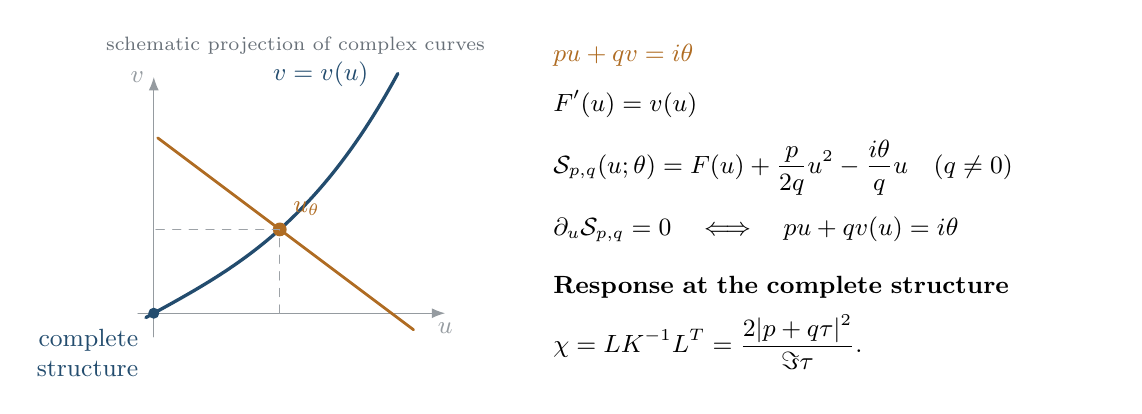
\begin{tikzpicture}[font=\small,line cap=round,>=Latex]
  \begin{scope}[shift={(-5.6,-1.1)}]
    \draw[->,mpgray!70] (-.2,0)--(3.7,0) node[below] {$u$};
    \draw[->,mpgray!70] (0,-.3)--(0,3.0) node[left] {$v$};
    \draw[mpblue,line width=1.2pt,domain=-.1:3.1,samples=80]
      plot (\x,{.55*\x+.045*\x*\x*\x});
    \draw[mpochre,line width=1pt] (.05,2.22682)--(3.3,-.21068);
    \fill[mpblue] (0,0) circle (2pt) node[below left=3pt,align=right] {complete\\structure};
    \fill[mpochre] (1.6,1.06432) circle (2.5pt);
    \draw[mpgray!65,dashed] (1.6,0)--(1.6,1.06432)--(0,1.06432);
    \node[above left=2pt,text=mpblue] at (2.9,2.697) {$v=v(u)$};
    \node[above right=2pt,text=mpochre] at (1.6,1.06432) {$u_\theta$};
    \node[text=mpgray,font=\scriptsize] at (1.8,3.4) {schematic projection of complex curves};
  \end{scope}
  \node[align=left,text width=7.0cm,anchor=west] at (-.65,.25) {%
    \textcolor{mpochre}{$\displaystyle pu+qv=i\theta$}\\[7pt]
    $\displaystyle F'(u)=v(u)$\\[7pt]
    $\displaystyle\mathcal S_{p,q}(u;\theta)
       =F(u)+\frac{p}{2q}u^2-\frac{i\theta}{q}u\quad(q\ne0)$\\[7pt]
    $\displaystyle\partial_u\mathcal S_{p,q}=0
       \quad\Longleftrightarrow\quad pu+qv(u)=i\theta$\\[10pt]
    \textbf{Response at the complete structure}\\[5pt]
    $\displaystyle\chi=LK^{-1}L^T
       =\frac{2|p+q\tau|^2}{\Im\tau}$.};
\end{tikzpicture}
\caption[Dehn filling in peripheral phase space]{Local Dehn filling as an intersection in the complex peripheral
holonomy space. The drawing records the intersection condition; it is
not a real slice of the complex deformation curve. Here $u,v$ are
logarithms of multipliers, $\theta=0$ is the complete structure, and
$\theta=2\pi$ gives smooth filling when the branch has that geometric
completion. The Hessian response formula assumes the
nondegenerate positive angle maximum specified in the text.}
\label{fig:mono-dehn-filling}
\end{figure}
% END INLINE FIGURE

\subsection{The Neumann--Zagier coefficients through sixth order}

Series inversion of~\eqref{eq:dehncone} gives
\begin{equation}
 u_\theta=\frac{i\theta}{A}
   +\frac{iqc_3\theta^3}{A^4}
   +i\theta^5\left(\frac{3q^2c_3^2}{A^7}
                         -\frac{qc_5}{A^6}\right)+\cdots.
 \label{eq:dehninversion}
\end{equation}
Substitution in the action, or integration of the envelope derivative,
gives
\begin{equation}
 \mathcal S^*(\theta)=\frac{\theta^2}{2qA}
  +\frac{c_3\theta^4}{4A^4}
  +\frac{\theta^6}{6}
       \left(\frac{3qc_3^2}{A^7}-\frac{c_5}{A^6}\right)+\cdots.
 \label{eq:dehncriticalseries}
\end{equation}
Taking half its imaginary part yields the volume loss
\begin{align}
 V_0-V_{p,q}(\theta)
 ={}&\frac{B\theta^2}{4|A|^2}
       -\frac{\theta^4}{8}\Im\frac{c_3}{A^4}\notag\\
    &-\frac{\theta^6}{12}
       \Im\left(\frac{3qc_3^2}{A^7}-\frac{c_5}{A^6}\right)
       +O(|A|^{-8}).
 \label{eq:dehnconeloss}
\end{align}
Here the displayed remainder is a long-slope estimate for bounded
$\theta$, on the common holonomy neighborhood constructed above.
The uniform analytic inverse expands in $i\theta/A$ with coefficients
analytic in the bounded parameter $q/A$; the next volume terms are
therefore $O(|A|^{-8})$. Since $q/A$ is bounded, the three displayed terms have
orders $|A|^{-2},|A|^{-4},|A|^{-6}$. For a fixed slope and
$\theta\to0$, the corresponding Taylor remainder is $O(\theta^8)$.

For the smooth hyperbolic filling $M_{p/q}$ this becomes
\begin{align}
 \boxed{\begin{aligned}
 V_0-\Vol(M_{p/q})
 ={}&\frac{\pi^2B}{|A|^2}
       -2\pi^4\Im\frac{c_3}{A^4}\\
    &-\frac{16\pi^6}{3}
       \Im\left(\frac{3qc_3^2}{A^7}-\frac{c_5}{A^6}\right)
       +O(|A|^{-8}).
 \end{aligned}}
 \label{eq:dehnsmoothloss}
\end{align}
These are the Neumann--Zagier coefficients, with the multiplier
normalization fixed explicitly~\cite[Section 6]{NeumannZagier}.
In particular the leading loss is $\pi^2/Q(p,q)$, and the quartic
term detects the first nonlinear deformation coefficient $c_3$.

\subsection{Computing the quartic coefficient from angle-volume derivatives}

The comparison supplies a more detailed computational identity.
Keep $K,L,\chi$ as above, and write
\[
 T_3=D^3\mathscr V(0),\qquad T_4=D^4\mathscr V(0),\qquad
 e=\frac{K^{-1}L^T}{\chi},\qquad
 R=K^{-1}-\frac{K^{-1}L^TLK^{-1}}{\chi}.
\]
Let $t=T_3(e,e,\cdot)$ be the resulting column covector. Solving
the constrained stationary equation to second order gives
\[
 x_\theta=\theta e+\frac{\theta^2}{2}Rt+O(\theta^3).
\]
Indeed $Le=1$, $LR=0$, and $RK$ is the identity on
$\ker L$. Inserting this expression into the Taylor expansion of
$\mathscr V$ gives
\begin{align}
 V_{p,q}(\theta)={}&V_0-\frac{\theta^2}{2\chi}
  +\frac{\theta^3}{6}T_3[e,e,e]\notag\\
  &+\frac{\theta^4}{24}
       \left(T_4[e,e,e,e]+3t^TRt\right)+O(\theta^5).
 \label{eq:dehnquartictensors}
\end{align}
The cross term with the unknown cubic displacement vanishes because
that displacement is in $\ker L$ and $Ke=L^T/\chi$.
The remaining quadratic-displacement terms combine to $t^TRt/8$.
Evenness of the geometric branch then removes the odd coefficients
and improves the remainder to $O(\theta^6)$. Comparison with
\eqref{eq:dehnconeloss} yields
\begin{equation}
 \boxed{T_3[e,e,e]=0,\qquad
 T_4[e,e,e,e]+3t^TRt
      =3\Im\frac{c_3}{(p+q\tau)^4}.}
 \label{eq:dehnquarticdictionary}
\end{equation}
Thus $c_3$ can be accessed from derivatives of the angle-volume
functional by varying the slope. The correction $3t^TRt$ accounts
for readjustment of all other angles. Keeping only the raw fourth
derivative would miss that response.

\subsection{The closed quantum-volume statement and its local consequence}

A precise closed-manifold analogue is the Chen--Yang volume conjecture.
At the specified root $\zeta_r=e^{2\pi i/r}$, with $r$ odd, its
absolute-growth statements are
\begin{equation}
 \frac{4\pi}{r}\log|\mathrm{RT}_r(N;\zeta_r)|\longrightarrow\Vol(N),
 \qquad
 \frac{2\pi}{r}\log\mathrm{TV}_r(N;\zeta_r)\longrightarrow\Vol(N).
 \label{eq:closedquantumvolume}
\end{equation}
The root and normalization matter; these are the Chen--Yang versions
for hyperbolic manifolds~\cite{ChenYang}. We use absolute growth
to avoid mixing the different Chern--Simons sign conventions in
the literature.

For a boundary state whose geometric semiclassical phase satisfies
\[
 \Phi(u)=\Phi_0+\frac12F(u),\qquad \Im\Phi_0=V_0,
\]
the filling phase is
\begin{equation}
 \mathcal T_\theta(u)=\Phi_0+\frac12\mathcal S_{p,q}(u;\theta).
 \label{eq:dehnquantumphase}
\end{equation}
Possible real framing constants do not alter its imaginary part.
With $\hbar_r=4\pi i/r$, Proposition~\ref{prop:dehncriticalvalue}
immediately gives
\begin{equation}
 \left|e^{\mathcal T_\theta(u_\theta)/\hbar_r}\right|
   =\exp\left(\frac{r}{4\pi}V_{p,q}(\theta)\right).
 \label{eq:dehnquantumexponent}
\end{equation}
In particular, the deformation of the geometric exponential is
\begin{equation}
 \log\left|\frac{e^{\mathcal T_\theta(u_\theta)/\hbar_r}}
                         {e^{\Phi_0/\hbar_r}}\right|
       =-\frac{r}{4\pi}\bigl(V_0-V_{p,q}(\theta)\bigr).
 \label{eq:dehnquantumresponse}
\end{equation}
Every classical coefficient in~\eqref{eq:dehnconeloss} therefore
appears with precisely the required quantum exponential coefficient.
At $\theta=2\pi$, Yoshida's complex-volume formula has this
normalization; see the unnumbered filling formula and the potential
normalization (5.9) on~\cite[p.~456]{WongYangDehn}.
Quadratic and linear filling kernels also appear explicitly
in~\cite[equations (12)--(14)]{GangRomoYamazaki}; their boundary
coordinates and level conventions must be converted before numerical
coefficients are compared.

\begin{proposition}[Conditional local quantum transfer]
\label{prop:dehnquantumconditional}
Suppose an exact surgery representation for a specified quantum
invariant has, near the geometric branch, phase
$\mathcal T_\theta$ and a uniform classical-symbol expansion of
its amplitude. Suppose the geometric critical point is nondegenerate,
its steepest-descent cycle occurs with nonzero coefficient in the
specified integration cycle, the net leading stationary-phase
coefficient of that geometric sector is uniformly bounded away
from zero, and the remaining integral or sum is
exponentially smaller, uniformly on a chosen compact deformation
interval. Then stationary phase gives the volume exponent
\eqref{eq:dehnquantumexponent} for the full invariant, with a
uniform expansion on that interval. Without the last global
condition, the same statement holds for the specified local
geometric contribution.
\end{proposition}

\begin{proof}
At the geometric critical point,
\[
 \mathcal T_\theta''(u_\theta)
   =\frac{p+qv'(u_\theta)}{2q}\ne0.
\]
Uniform stationary phase on the stipulated cycle gives a nonzero
amplitude times $e^{\mathcal T_\theta(u_\theta)/\hbar_r}$,
with powers of $r^{-1}$ and a Gaussian power of $r$ according
to the normalization of the kernel. Such powers contribute only
$O(\log r/r)$ to normalized logarithmic growth. The exponential
gap permits the addition of the remaining terms without changing
the leading growth. The critical-value proposition identifies the
exponent with the geometric volume.
\end{proof}

For a general knot this proposition identifies the needed analytic
input; it does not establish that input from a complete-point
Kashaev asymptotic alone. A value at $u=0$ does not provide a
uniform boundary-state expansion near $0$, and a local critical
point does not by itself specify its coefficient in the global
surgery sum. The regular tetrahedral Airy formula in
Section~\ref{sec:quantumAiry} concerns a different integral and
does not supply that missing manifold-level information.

\subsection{The Gaussian factor and the torsion surgery formula}

The derivative of the filling map is
\begin{equation}
 D_*:=p+qv'(u_\theta),\qquad
 \frac{\dd u_\theta}{\dd\theta}=\frac{i}{D_*},\qquad
 \mathcal S_{uu}(u_\theta;\theta)=\frac{D_*}{q}.
 \label{eq:dehnjacobian}
\end{equation}
Thus the same quantity controls the classical susceptibility and
the Gaussian surgery integral. With the usual square-root
normalization of the boundary Fourier kernel, its contribution
has dependence $D_*^{-1/2}$, up to the common normalization and
phase choices. A full amplitude also contains the boundary-state
torsion and a solid-torus factor.

More precisely, suppose $\theta=2\pi$ gives a smooth hyperbolic filled
manifold and the representation is its holonomy. Assume its adjoint
representation is acyclic and its restriction to the compact core is
regular for both $\mu$ and $p\mu+q\lambda$: the peripheral invariant
vector paired with either curve supplies a basis of the one-dimensional
twisted $H_1$, with the compatible boundary basis in $H_2$.
In the local holonomy chart this requires $D_*\ne0$; the core is
loxodromic, so $\sinh(w/2)\ne0$. The change-of-peripheral-curve
and surgery formulas for adjoint Reidemeister torsion then give
\begin{align}
 \operatorname{Tor}_{p\mu+q\lambda}(M_u)
   &=\bigl(p+qv'(u)\bigr)\operatorname{Tor}_\mu(M_u),\notag\\
 \operatorname{Tor}(M_{p/q})
   &=\frac{\operatorname{Tor}_{p\mu+q\lambda}(M_u)}
               {4\sinh^2(w/2)},\qquad
 w=\rho u+\sigma v.
 \label{eq:dehntorsionsurgery}
\end{align}
These are understood up to the standard torsion signs and
consistent choices of square root. They are the identities
used in~\cite[equations (5.16) and (5.23)]{WongYangDehn}.
For the general regularity and change-of-curve statements, see
\cite[Propositions 5.13--5.14]{PortiTorsionSurvey}; its
Proposition 4.23(b), specialized to the adjoint representation
$(k_1,k_2)=(2,0)$, gives the surgery factor up to the torsion sign.
Consequently the expected full geometric amplitude is proportional to
\begin{equation}
 \boxed{
 \frac{2\sinh(w/2)}
      {\sqrt{\bigl(p+qv'(u)\bigr)\operatorname{Tor}_\mu(M_u)}}
       =\frac{1}{\sqrt{\operatorname{Tor}(M_{p/q})}}.}
 \label{eq:dehngaussiantorsion}
\end{equation}
The identity shows what must accompany the boundary Hessian.
Matching the Gaussian factor alone would leave out both the cusp
torsion and the solid-torus amplitude. This one-loop comparison
uses more information than the classical volume exponent.
The closed-manifold torsion in this formula is evaluated at smooth
filling; it is not being assigned to a generic cone holonomy.
At the cusp endpoint $\theta=0$ the solid-torus factor vanishes,
so a uniform quantum statement including that endpoint requires
a separate normalization and analysis. The compact parameter
interval in Proposition~\ref{prop:dehnquantumconditional} is
subject to its nonvanishing-amplitude hypothesis.

\subsection{A figure-eight benchmark and the scope of the conclusion}

For the figure-eight knot complement, in the standard peripheral
basis Neumann--Zagier compute~\cite[equation (68)]{NeumannZagier}
\begin{equation}
 v(u)=2\sqrt3\,i\left(u+\frac{u^3}{3}
                    +\frac{23u^5}{180}+O(u^7)\right).
 \label{eq:figureeightNZcoefficients}
\end{equation}
Thus $\tau=2\sqrt3\,i$, $c_3=2i/\sqrt3$, and
$c_5=23i/(30\sqrt3)$. The first two volume-loss terms are
\begin{align}
 V_0-\Vol(M_{p/q})={}&\frac{2\sqrt3\,\pi^2}{p^2+12q^2}\notag\\
 &-\frac{4\pi^4}{\sqrt3}
  \frac{p^4-72p^2q^2+144q^4}{(p^2+12q^2)^4}
  +O\bigl((p^2+q^2)^{-3}\bigr).
 \label{eq:figureeightfillingloss}
\end{align}
This agrees directly with the expansion following equation (68)
in~\cite{NeumannZagier}. The angle-Hessian response is correspondingly
\[
 \chi=\frac{p^2+12q^2}{\sqrt3}.
\]

An independent calculation starts with the two regular ideal tetrahedra
and their Lobachevsky volume. In the Neumann--Zagier presentation their
shapes $z_1,z_2$ satisfy
\[
 z_1z_2(z_1-1)(z_2-1)=1,\qquad
 u=\log\bigl(z_2(1-z_1)\bigr),\qquad
 v=2\log\bigl(z_1(1-z_1)\bigr).
\]
Eliminating the shapes from these equations gives the local peripheral
relation
\[
 \cosh(v/2)=1+\cosh u-\cosh(2u).
\]
Equivalently, with the eigenvalue variables
$m=e^{u/2}$ and $l=-e^{v/2}$, it is
$l+l^{-1}=m^4-m^2-2-m^{-2}+m^{-4}$, the nonabelian
figure-eight $A$-polynomial relation in this choice of signs.
The sign in $l$ is essential: its complete value is $-1$ whereas
$v(0)=0$. The equation and the chosen tangent $v'(0)=2\sqrt3\,i$
recover the cubic and quintic coefficients above. This is a local
branch calculation, not a classification of the global curve or of fillings.

Use $\alpha_i=\arg z_i$, $\beta_i=-\arg(1-z_i)$, and
$\gamma_i=\pi-\alpha_i-\beta_i$. Choose the independent variations
$\xi=(\delta\alpha_1,\delta\beta_1,\delta\alpha_2)$.
The edge equation then makes the six angle variations
\[
 E\xi=(\xi_1,\xi_2,-\xi_1-\xi_2,
       \xi_3,\xi_1-\xi_2+\xi_3,-\xi_1+\xi_2-2\xi_3).
\]
At the complete structure all six angles are $\pi/3$.
Since $\Lambda''(\alpha)=-\cot\alpha$, direct differentiation gives
\begin{equation}
 K=\frac1{\sqrt3}
 \begin{pmatrix}4&-1&3\\-1&4&-3\\3&-3&6\end{pmatrix},\qquad
 P=\begin{pmatrix}0&-1&1\\2&-2&0\end{pmatrix},\qquad
 P K^{-1}P^T=\frac1{\sqrt3}
 \begin{pmatrix}1&0\\0&12\end{pmatrix}.
 \label{eq:figureeightdirectHessian}
\end{equation}
This recovers the cusp shape directly from the optimizer.
Put $D_0=p^2+12q^2$. The unit angular-response vector is
\[
 e=\frac{(6q-p,-6q-p,p-6q)^T}{2D_0}.
\]
Using
\[
 \Lambda'''(\pi/3)=\frac43,\qquad
 \Lambda''''(\pi/3)=-\frac8{3\sqrt3},
\]
the six entries of $Ee$ occur in opposite pairs, so
$T_3[e,e,e]=0$. Direct contraction of the fourth derivative and
the constrained inverse-Hessian correction gives
\begin{equation}
 T_4[e,e,e,e]+3t^TRt
   =\frac{2\sqrt3\,(p^4-72p^2q^2+144q^4)}{D_0^4}.
 \label{eq:figureeightdirectquartic}
\end{equation}
Multiplying by $\theta^4/24$ and setting $\theta=2\pi$ gives
the quartic filled-volume term in~\eqref{eq:figureeightfillingloss}
with the opposite sign, as required for volume rather than volume loss.
Thus the real optimization and the holomorphic series agree in a
calculation made directly from the tetrahedral volume derivatives.

For this example there is also a theorem about the actual quantum
invariants: Wong--Yang prove the leading RT asymptotic with relative
error $O(r^{-1})$, and the
RT/TV volume conjectures for every hyperbolic rational Dehn filling
of the figure-eight knot~\cite[Theorems 1.1 and 1.2]{WongYangDehn}.
Their leading amplitude is the inverse square root of adjoint torsion,
with their specified overall constant. Thus the local consistency
calculation above is contained in a stronger result in that example.
The present discussion reorganizes the comparison around volume
optimization and its derivatives; it does not produce a new case
of the quantum-volume conjecture.

For a general knot, the unconditional results here are the classical
critical-value identity and its coefficient dictionary. The quantum
conclusion for a specified local geometric contribution follows under
the stated stationary-phase hypotheses. Passing to the full invariant
requires control of its exact surgery representation and all competing
contributions. One should first keep the filling slope fixed while
taking $r\to\infty$, and then study the long-slope coefficients.
A simultaneous limit in which the slope grows with $r$ requires
uniform estimates not supplied by separate fixed-slope expansions.

The computational companion in
\path{experiments/quantum_surgery/README.md}, with output at
\path{artifacts/quantum_surgery/result.json}, checks finite formal
series, canonical-coordinate identities, and the figure-eight
angle-Hessian contractions in exact arithmetic. These fixtures
check the displayed coefficient algebra. They do not compute a
filled hyperbolic manifold or an exact quantum invariant, and do
not establish convergence, a global integration cycle, or its
noncancellation.

\subsection{The symplectic pairing behind the calculation}
\label{sec:NZsymplectic}

The pairing in Neumann--Zagier is the structure behind the preceding
formulas. It identifies the peripheral variables as conjugate coordinates,
makes the geometric deformation locus Lagrangian, and fixes the canonical
transformation for Dehn filling. We record the normalization explicitly,
since interchanging meridian and longitude or using eigenvalue rather
than multiplier logarithms changes the displayed signs or factors.

\subsubsection{From the tetrahedra to the boundary intersection form}

For $n$ ideal tetrahedra introduce independent ambient coordinates
\[
 Z_j=\log z_j,\qquad W_j=\log(1-z_j),\qquad
 \Omega_{\rm tet}=\sum_{j=1}^n\dd Z_j\wedge\dd W_j.
\]
The actual shapes satisfy $e^{Z_j}+e^{W_j}=1$. Their product is a
complex Lagrangian of dimension $n$ in this $2n$-dimensional phase space.
The logarithmic edge equations and peripheral holonomies are affine
linear functions of $X=(Z_1,\ldots,Z_n,W_1,\ldots,W_n)^T$.

Let $C_\lambda,C_\mu$ be the longitude and meridian coefficient rows,
let $R_E$ be the edge-equation matrix, and set
\[
 J_{2n}=\begin{pmatrix}0&I_n\\-I_n&0\end{pmatrix},\qquad
 U=\begin{pmatrix}C_\lambda\\C_\mu\\R_E\end{pmatrix}.
\]
For a triangulated manifold with $h$ torus cusps, the original matrix identity is
\begin{equation}
 \boxed{U J_{2n}U^T
 =2\begin{pmatrix}0&I_h&0\\-I_h&0&0\\0&0&0\end{pmatrix}.}
 \label{eq:NZmatrixpairing}
\end{equation}
This is~\cite[Theorem 2.2, equation (21)]{NeumannZagier}, in their
longitude--meridian row order. They normalize the coefficient-row
pairing as $\langle a,b\rangle=\tfrac12aJ_{2n}b^T$.
Equivalently, the unnormalized coefficient pairing of peripheral curves
is twice their oriented intersection number; edge rows pair to zero
with one another and with all peripheral rows. The topological
interpretation is proved in their Section 3. A geometric construction
of symplectic bases is given in~\cite{MathewsPurcellSymplectic}.

The vanishing edge-edge pairings say that the linear constraints
Poisson-commute. Since $\operatorname{rank}R_E=n-h$, their
coisotropic reduction has complex dimension $2h$. Corollary 2.4 of
\cite{NeumannZagier} identifies the reduced form as
\begin{equation}
 \boxed{\Omega_\partial=\frac12\sum_{i=1}^h
                   \dd v_i\wedge\dd u_i,\qquad
 \alpha_\partial=\frac12\sum_{i=1}^h v_i\,\dd u_i,
 \qquad \dd\alpha_\partial=\Omega_\partial.}
 \label{eq:NZboundarysymplectic}
\end{equation}
Locally near the regular geometric point, imposing the edge equations
on the tetrahedral Lagrangian and reducing gives the geometric
deformation Lagrangian $\mathcal L_M$ in boundary holonomy space.
For a modern formulation of the reduction, see~\cite{DimofteVeen}.
The symplectic form lives on the ambient boundary phase space;
its pullback to $\mathcal L_M$ is zero.

\subsubsection{The potential and the volume primitive}

Writing $v=v(u)$ on the geometric branch, Lagrangianity gives
\begin{equation}
 \sum_i\dd v_i\wedge\dd u_i=0
 \quad\Longleftrightarrow\quad
 \frac{\partial v_i}{\partial u_j}
       =\frac{\partial v_j}{\partial u_i}.
 \label{eq:NZreciprocity}
\end{equation}
Thus $\sum_i v_i\,\dd u_i=\dd F$ locally, and
$\alpha_\partial|_{\mathcal L_M}=\dd(F/2)$.
This is the reciprocity and potential statement of
\cite[Theorem 3]{NeumannZagier}. For one cusp the existence of a
primitive is automatic once $v=v(u)$; the substantial content is
the triangulation-level pairing and, for several cusps, the
symmetry of the mixed derivatives. In the original normalization,
$\Phi_{\rm NZ}=2F$, whereas the complex-volume phase used above is
$\Phi=\Phi_0+F/2$.

For one cusp write
\[
 u=x+iy,\qquad v=r+is.
\]
The real volume one-form is an exact modification of the imaginary
part of the symplectic primitive:
\begin{equation}
 \beta=\frac12(r\,\dd y-x\,\dd s)
       =\Im\alpha_\partial-\frac12\dd(xs),\qquad
 \dd\beta=\Im\Omega_\partial.
 \label{eq:NZvolumeprimitive}
\end{equation}
It is therefore closed on $\mathcal L_M$. Integrating it gives exactly
\eqref{eq:NZrealvolume}. The factor $1/2$ can also be seen from
the leading--trailing angle variations: angular holonomy varies by
twice the boundary intersection number, while volume varies by the
real holonomy~\cite[Lemma 4.4 and Proposition 5.4]{FuterGueritaud}.
The same pairing thus supplies the real optimization differential
and the holomorphic generating function.

\subsubsection{Filling as a canonical transformation}

Choose $\rho,\sigma\in\ZZ$ with $p\sigma-q\rho=1$ and use
the filling slope as the new meridian:
\begin{equation}
 a=pu+qv,\qquad b=\rho u+\sigma v,\qquad
 \frac12\dd b\wedge\dd a=\frac12\dd v\wedge\dd u.
 \label{eq:NZcanonicalfilling}
\end{equation}
For $q\ne0$, the type-I generating function is
\begin{equation}
 \boxed{G(u,a)=\frac{p}{4q}u^2-\frac{ua}{2q}
                         +\frac{\sigma}{4q}a^2.}
 \label{eq:NZcanonicalkernel}
\end{equation}
Indeed, $v=(a-pu)/q$ and $b=(\sigma a-u)/q$ give the exact identity
\begin{equation}
 \dd G=\frac12b\,\dd a-\frac12v\,\dd u.
 \label{eq:NZgeneratingidentity}
\end{equation}
Thus
\[
 \widetilde\Phi(a)=\operatorname{crit}_u\bigl(\Phi(u)+G(u,a)\bigr)
 \quad\text{satisfies}\quad
 \widetilde\Phi'(a)=\frac b2.
\]
The stationary equation is $a=pu+qv$. Setting $a=i\theta$ gives
\begin{equation}
 \widetilde\Phi(i\theta)
 =\Phi_0+\frac12\mathcal S^*_{p,q}(\theta)
          -\frac{\sigma\theta^2}{4q}.
 \label{eq:NZcanonicalaction}
\end{equation}
The last term is real, hence invisible to the volume. At
$\theta=2\pi$ it is $-\pi^2\sigma/q$, the framing term in
the Yoshida normalization used in~\cite[p.~456, formula preceding (5.9)]{WongYangDehn}.
The quadratic and linear terms of the surgery action are therefore
fixed by a symplectic change of coordinates.

The complementary core holonomy $b$ is conjugate to the filling
holonomy $a$. Along $a=i\theta$,
\[
 \dd\Im\widetilde\Phi
   =\Im\left(\frac12b\,i\dd\theta\right)
   =\frac12\Re b\,\dd\theta
   =-\frac12\ell_{\rm core}\,\dd\theta.
\]
This gives Schl\"afli and the real source
$j=\ell_{\rm core}/2$ in the canonical coordinates.

On the canonical relation, $G=(ab-uv)/4$, so
\begin{equation}
 \boxed{\widetilde\Phi-\frac{ab}{4}
                  =\Phi-\frac{uv}{4}.}
 \label{eq:NZinvariantpotential}
\end{equation}
Equivalently $\widetilde\Phi_{\rm NZ}-ab=\Phi_{\rm NZ}-uv$,
where $\widetilde\Phi_{\rm NZ}=4(\widetilde\Phi-\Phi_0)$.
The equality is local with consistently fixed logarithmic branches
and additive constants. It explains why the combination of potential
and peripheral product occurs in the complex-volume formula.
The differential of the boxed expression is the invariant one-form
$\tfrac14(v\,\dd u-u\,\dd v)$.

\subsubsection{Covariance of the filling coefficients}

The powers of $p+q\tau$ in~\eqref{eq:dehnsmoothloss} also have
a canonical-coordinate interpretation. Write the same geometric
Lagrangian in the new coordinates as
\[
 b(a)=\widetilde\tau a+\widetilde c_3a^3
                         +\widetilde c_5a^5+O(a^7).
\]
Using the inverse series of $a=pu+qv(u)$ gives, with $A=p+q\tau$,
\begin{align}
 \widetilde\tau&=\frac{\rho+\sigma\tau}{p+q\tau},
 &\Im\widetilde\tau&=\frac{\Im\tau}{|p+q\tau|^2},\notag\\
 \widetilde c_3&=\frac{c_3}{A^4},
 &\widetilde c_5&=\frac{c_5}{A^6}-\frac{3qc_3^2}{A^7}.
 \label{eq:NZcoefficientcovariance}
\end{align}
The cancellation in the cubic coefficient is
\[
 \sigma A-q(\rho+\sigma\tau)=1.
\]
It is exactly the symplectic determinant condition. Let
$\widetilde F(0)=0$ and $\widetilde F'=b$.
Since $\Re a=0$ on the cone locus, the real boundary correction
in the new coordinates vanishes. Therefore
\begin{equation}
 V_{p,q}(\theta)-V_0
  =\frac12\Im\widetilde F(i\theta)
  =-\frac{\theta^2}{4}\Im\widetilde\tau
    +\frac{\theta^4}{8}\Im\widetilde c_3
    -\frac{\theta^6}{12}\Im\widetilde c_5+\cdots.
 \label{eq:NZvolumenewpolarization}
\end{equation}
This is the previously computed volume expansion in filling
coordinates. The cubic coefficient has a weight-$-4$ covariance
law under a peripheral basis change; this alone does not assert
that it is a modular form as a function of cusp shape.
The pairing fixes the transformation laws, while the actual values
of $c_3,c_5,\ldots$ describe nonlinear geometry of $\mathcal L_M$.

\subsubsection{An exact Hessian and Monge--Ampere identity}

There is a useful strengthening of~\eqref{eq:cuspmatrixHessian}.
Eliminate internal angles at fixed peripheral angular holonomies,
writing
\[
 \overline V(y,s)=\max_{P\xi=(y,s)}\mathscr V(\xi).
\]
All statements are local in the positive geometric neighborhood,
where the maximum is interior and nondegenerate. Let
$K(\xi)=-D^2\mathscr V(\xi)>0$ at the maximizing point.
The boundary intersection pairing gives $\operatorname{rank}P=2$,
so the constrained implicit-function theorem supplies a unique nearby
interior maximizer for every sufficiently small $(y,s)$.
Stationarity in the internal directions enforces real edge gluing,
so this maximizer lies on the same deformation branch $v=v(u)$.
The map $u=x+iy\mapsto(y,\Im v(u))$ is locally invertible because
$\Im v'(0)=B>0$. It therefore identifies the angular boundary
parameters with that geometric branch, rather than with an unrelated
constrained family.
The Schur-complement identity for the linear constraints is
\begin{equation}
 -D^2\overline V=(P K(\xi)^{-1}P^T)^{-1}.
 \label{eq:NZreducedHessian}
\end{equation}
Set $T=v'(u)=A_0+iB_0$, with $B_0>0$ near the complete point.
The volume differential and Cauchy--Riemann equations give
\[
 \overline V_y=\frac r2,\qquad
 \overline V_s=-\frac x2,\qquad
 \dd s=B_0\dd x+A_0\dd y,\qquad
 \dd r=A_0\dd x-B_0\dd y.
\]
Solving these two linear differential equations yields
\begin{equation}
 \boxed{-D^2\overline V
 =\frac1{2B_0}\begin{pmatrix}|T|^2&-A_0\\-A_0&1\end{pmatrix},
 \qquad \det(-D^2\overline V)=\frac14.}
 \label{eq:NZMongeAmpere}
\end{equation}
Equivalently,
\begin{equation}
 P K(\xi)^{-1}P^T
  =\frac2{\Im v'(u)}
       \begin{pmatrix}1&\Re v'(u)\\
                       \Re v'(u)&|v'(u)|^2\end{pmatrix}.
 \label{eq:NZnonlinearresponse}
\end{equation}
The determinant-$4$ identity holds throughout this local branch.
At $u=0$ it reduces to the cusp formula already derived.
For a filling path it gives the exact response
\begin{equation}
 V_{p,q}''(\theta)
   =-\frac{\Im v'(u_\theta)}
            {2|p+qv'(u_\theta)|^2},
 \label{eq:NZexactcurvature}
\end{equation}
in agreement with~\eqref{eq:dehnenvelope}.

For a geometric interpretation of the positive Hessian metric
$g=-D^2\overline V$, multiplication by $i$ in the $u$-coordinate
induces, in coordinates $(y,s)$,
\[
 J_T=\frac1{B_0}
      \begin{pmatrix}-A_0&1\\-|T|^2&A_0\end{pmatrix},
 \qquad J_T^2=-I.
\]
Then
\begin{equation}
 \omega_{\rm ang}=-\frac12\dd y\wedge\dd s,\qquad
 g(X,Y)=\omega_{\rm ang}(X,J_TY),\qquad
 g=\frac{B_0}{2}(\dd x^2+\dd y^2).
 \label{eq:NZcompatiblemetric}
\end{equation}
This real area form comes from the angular polarization and the
positive complex tangent. It is not the pullback of
$\Omega_\partial$, which vanishes on the geometric Lagrangian.
Nor has it been identified with the earlier
Thurston--Deligne--Mostow complex hyperbolic metric.

For completeness, assume the same positive complete triangulation and
regular deformation hypotheses with $h$ torus cusps, and use all $2h$
peripheral angular constraints. Their matrix $P$ has rank $2h$ by the
boundary intersection pairing. Let
$T=(\partial v_i/\partial u_j)=A_0+iB_0$.
It is symmetric, and $B_0>0$ near the complete point. In coordinates
$(y,s)=(\Im u,\Im v)$ the same calculation gives
\begin{equation}
 -D^2\overline V
  =\frac12\begin{pmatrix}
   B_0+A_0B_0^{-1}A_0&-A_0B_0^{-1}\\
   -B_0^{-1}A_0&B_0^{-1}
   \end{pmatrix},\qquad
 \det(-D^2\overline V)=4^{-h}.
 \label{eq:NZmulticuspHessian}
\end{equation}
At the complete structure $T$ is diagonal, with the individual cusp
shapes on the diagonal. Coupling between distinct cusps appears in
higher derivatives of the even Neumann--Zagier potential, for example
through terms $u_i^2u_j^2$.

\subsubsection{The quantum Gaussian as a half-density transformation}

Let a geometric boundary state have leading form
$A_0(u)e^{\Phi(u)/\hbar}$, with $\Phi'=v/2$.
A quantization of the canonical transformation uses the exponential
kernel $e^{G(u,a)/\hbar}$ and its mixed-derivative normalization.
The relevant derivatives are
\[
 -G_{ua}=\frac1{2q},\qquad
 (\Phi+G)_{uu}=\frac{p+qv'(u)}{2q}.
\]
The kernel normalization divided by the stationary Gaussian therefore
has the dependence
\begin{equation}
 \boxed{\sqrt{\frac{-G_{ua}}{(\Phi+G)_{uu}}}
    =\frac1{\sqrt{p+qv'(u)}}
    =\sqrt{\frac{\dd u}{\dd a}}.}
 \label{eq:NZhalfdensity}
\end{equation}
Universal powers of $\hbar$, phases, and square-root branches are
fixed by the chosen integral convention. The displayed dependence is
the transformation law for a half-density along $\mathcal L_M$.
It is exactly the law obeyed by the inverse square root of peripheral
torsion in~\eqref{eq:dehntorsionsurgery}. The extra
$2\sinh(b/2)$ factor comes from the solid torus and is additional
input. Explicit quantum filling kernels appear
in~\cite[equations (12)--(14)]{GangRomoYamazaki}.

The symplectic structure fixes the conjugate variables, the canonical
generating function, and this Gaussian Jacobian. It does not select
the integration cycle or prove that the geometric contribution
survives cancellation in the exact quantum invariant. The analytic
hypotheses in Proposition~\ref{prop:dehnquantumconditional} remain
necessary for that conclusion.



\monographpart{Curves, trace formulas, and quotients}{Cutting and gluing geodesics produces identities and twist integrals. Twisted trace formulas retain the multicurve coefficients and their lengths.}

\section{Unfolding and the problem of finding constant series}
\label{sec:unfolding}

\subsection{What a volume computation determines}

Let $\Gamma$ be the mapping class group and let $\gamma$ be a fixed curve
or multicurve class. For an appropriate nonnegative or absolutely integrable
function, the basic unfolding identity is
\begin{equation}
 \int_{\Gamma\backslash\T}
 \sum_{\delta\in\Gamma\gamma}F(\ell_\delta(X))\,\dV(X)
 =\int_{\Stab(\gamma)\backslash\T}
             F(\ell_\gamma(X))\,\dV(X).
 \label{eq:unfold}
\end{equation}
Multiplicity conventions belong in the stabilizer. This identity is just
integration over coset translates of a fundamental domain; it does not
require the curves in the orbit to be simple.

Simplicity becomes important when evaluating the right side. If $\gamma$
is a disjoint simple multicurve, cut along it and use Fenchel--Nielsen
coordinates. Each twist period integrates to $\ell_j$, so the resulting
integral has factors $\prod_j\ell_j\,\dd\ell_j$ times WP volumes of the
components, with the relevant symmetry factors. This is the geometric
integration mechanism in Mirzakhani's volume recursion
\cite[Theorem 8.1]{MirzVolumes}.

Suppose a series $S(X)$ is independently known to be constant, say $C$.
Then
\begin{equation}
 C=\frac{1}{V_{g,n}}
       \int_{\M_{g,n}}S(X)\,\dV(X),
 \label{eq:recoverconstant}
\end{equation}
and unfolding can calculate its value. If constancy has not been proved,
the same quotient computes only its average. This is the precise logical
distinction behind the proposal to recover an identity from a volume.

On the punctured torus, for an unoriented essential simple curve orbit,
the stack-normalized formula is
\begin{equation}
 \int_{\M_{1,1}}\sum_{\alpha\text{ simple}}f(\ell_\alpha)\,\dV
       =\frac12\int_0^\infty x f(x)\,\dd x.
 \label{eq:torusunfold}
\end{equation}
For $f(x)=(1+e^x)^{-1}$, expand in $e^{-x}$ to obtain
\[
 \int_0^\infty\frac{x\,\dd x}{1+e^x}
   =\sum_{m\ge1}\frac{(-1)^{m-1}}{m^2}=\frac{\pi^2}{12}.
\]
The integral of the series is $\pi^2/24$; division by
$V_{1,1}=\pi^2/12$ gives $C=1/2$. Its pointwise constancy is McShane's
theorem~\cite{McShane}:
\begin{equation}
 \sum_{\alpha\text{ simple, unoriented}}
                 \frac{1}{1+e^{\ell_\alpha(X)}}=\frac12.
 \label{eq:mcshane}
\end{equation}
The tetrahedral volume calculation and the covering argument provide an
independent route to the volume used in this normalization check.

\subsection{Operations that preserve constancy}

There is indeed a large closure of any known collection of identities.
Finite linear combinations preserve constancy. So do absolutely convergent
parameter integrals and locally uniformly convergent differentiations of
identities on an identified parameter family. Products of identities give
constant double series when Tonelli's theorem or absolute convergence
applies. These are useful mechanisms for constructing new kernels.

Their geometric interpretation needs to be retained. A product usually
indexes pairs of curves that may intersect; it is not automatically a
disjoint-multicurve sum. A parameter derivative also differentiates lengths
if the metric varies with that parameter. In particular, differentiating
a constant series with respect to the metric gives the one-form identity
\begin{equation}
 \sum_\gamma F'(\ell_\gamma)\,\dd\ell_\gamma=0,
 \label{eq:derivativeidentity}
\end{equation}
assuming sufficient local uniform control. It does not generally give
another scalar identity by differentiating only the displayed weight.

Two possible tests for a proposed constant series follow. One can try to
show that~\eqref{eq:derivativeidentity} vanishes on a spanning set of tangent
directions. Alternatively, if $S\in L^2$ and its mean is $\overline S$, then
\begin{equation}
 \int_{\M}(S-\overline S)^2\,\dV=0
 \label{eq:variance}
\end{equation}
proves constancy almost everywhere, and everywhere if $S$ is continuous.
The second-moment calculation involves pairs of curves, including their
intersection patterns. It can be substantially harder than the first
unfolding integral.

Thus a useful search for further identities should ask for more than
formal closure: a natural index set, a manageable positive weight, a
geometric partition or telescoping mechanism, and a convergence proof.
The constructions in Sections~\ref{sec:figures} and~\ref{sec:exacttwist}
illustrate these requirements.

\subsection{Other established constant series}

There are also constant series with substantially different kernels.
For example, write
\[
 \mathcal L(x)=\operatorname{Li}_2(x)+\tfrac12\log x\log(1-x)
\]
for the Rogers dilogarithm on $(0,1)$, extended continuously to its
endpoints, and define
\begin{align*}
 D(r)={}&\mathcal L\bigl(\sech^2(r/2)\bigr)\\
 &+2\mathcal L\left(\frac{1+e^{-r}}2\right)
  -2\mathcal L\left(\frac{1-e^{-r}}2\right).
\end{align*}
Hu--Tan's punctured-torus identity is
\begin{equation}
 \sum_{\alpha\text{ simple, unoriented}}D(\ell_\alpha)=\frac{\pi^2}{2}.
 \label{eq:dilogtorus}
\end{equation}
The same paper treats a positive torus boundary~\cite[Theorems 1--2]{HuTan}.

For a closed surface of genus $g\ge2$, Luo--Tan give explicit dilogarithmic
weights $f(P),g(T)$ on embedded geometric pairs of pants and one-holed tori
such that
\begin{equation}
 \sum_P f(P)+\sum_T g(T)=8\pi^2(g-1)=\operatorname{Vol}(T^1X).
 \label{eq:luotan}
\end{equation}
Their construction partitions unit tangent directions~\cite{LuoTan}.
It illustrates another source of constant series: the invariant measure
being partitioned need not live only on a horocycle or a geodesic boundary.
The precise, longer subsurface weights are given in that reference.

\section{Figure-eight curves and simple lifts}
\label{sec:figures}

In this section surfaces have cusps or geodesic boundary and no cone
singularities.

\subsection{The pants trace relation}

Let $\gamma$ be a closed geodesic with exactly one transverse self-intersection,
not a proper iterate. Its two-lobed neighborhood is a pair of pants. After
tightening the cuffs, allow coincident cuff images in the ambient surface;
this occurs on a one-holed torus. If the three cuff lengths are $a,b,c$,
write
\[
 t_a=2\cosh(a/2),\quad t_b=2\cosh(b/2),\quad t_c=2\cosh(c/2).
\]
A cusp has positive trace $2$. For the figure-eight that wraps the $a$
and $b$ cuffs, the trace identity is
\begin{equation}
 \boxed{t_\gamma=t_at_b+t_c.}
 \label{eq:figuretrace}
\end{equation}
This is Rivin's pants relation~\cite[Theorem 1.3]{RivinFigures}. It also
follows directly from
$\tr(AB^{-1})=\tr A\,\tr B-\tr(AB)$ with the consistent signs of pants
holonomies; rewriting in positive traces produces the plus sign in
\eqref{eq:figuretrace}.

For pants with lengths $(a,b,0)$, the two figures that use the cusp as one
lobe have traces
\begin{equation}
 u=2t_a+t_b,\qquad v=t_a+2t_b,
 \qquad
 t_a=\frac{2u-v}{3},\quad t_b=\frac{2v-u}{3}.
 \label{eq:twofigures}
\end{equation}
Consequently any weight assigned to this pair of cuffs can be rewritten
as a weight in the two associated figure-eight lengths. This gives a
direct reindexing of a pants identity. It produces a paired-curve weight;
it does not automatically produce a universal function of one figure-eight
length.

\subsection{What the local double cover accomplishes}

Use pants generators $a,b$, with third cuff $c=(ab)^{-1}$ and figure
$\gamma=ab^{-1}$. Consider the connected double cover given by
\[
 \chi(a)=\chi(b)=1\in\ZZ/2\ZZ.
\]
Then $\chi(c)=\chi(\gamma)=0$. The $a,b$ cuffs each lift with degree two,
while $c$ has two degree-one lifts. The upstairs surface is a four-holed
sphere with cuff lengths
\begin{equation}
 (2a,2b,c,c).
 \label{eq:doublepants}
\end{equation}
The figure-eight has two closed degree-one lifts, each of which is simple.
One way to see this is to lift its two-loop spine: the lifted graph has
two vertices, and either lift uses one $a$ edge and one $b$ edge to form
a simple cycle.

The two lifted cycles meet at both vertices of that graph. Geometrically,
the two simple lifts intersect each other twice, once over each lift of
the original crossing. Thus two components of the lifted domain do not
mean a disjoint multicurve upstairs.

There is a further global issue: this particular character of the pants
group need not extend to the whole surface. A lobe that is zero in
$H_1(S;\ZZ/2\ZZ)$---for example, a separating lobe on a closed surface---
cannot be assigned value one by an ambient character.
Rivin proves a global substitute: a one-double-point geodesic has a simple
lift in a fourfold cover~\cite[Theorem 4.2]{RivinFigures}.

Even when a suitable cover exists, applying an entire simple-curve identity
upstairs and projecting downstairs introduces other projected topological
types, covering degrees, and multiplicities. Desingularization supplies
an important geometric tool, but selecting just the desired downstairs
curves requires additional accounting.

\subsection{The two types on a punctured torus}

On a once-punctured torus, a figure-eight has a unique essential simple
curve $\alpha$ disjoint from it. Its pants neighborhood has one peripheral
cuff and two parallel essential cuffs, which both tighten to $\alpha$.
Cutting along $\alpha$ gives pants of lengths $(a,a,0)$, where
$a=\ell_\alpha$ and $t=2\cosh(a/2)>2$.

There are exactly three unoriented figure-eight classes in these cut pants:
\begin{center}
\begin{tabular}{@{}p{0.42\textwidth}c c@{}}
\toprule
Lobes & Number & Positive trace\\
\midrule
One essential cuff and the cusp & $2$ & $3t$\\
Both essential cuff copies & $1$ & $t^2+2$\\
\bottomrule
\end{tabular}
\end{center}
The first two are exchanged by the hyperelliptic involution; call their
family $\mathcal N$. The third is hyperelliptic; call its family
$\mathcal H$. Equal lengths in the first row do not identify the two
free-homotopy classes. In torus homology the first family has a primitive
class up to sign and the second twice a primitive class, although its
geodesics are not proper iterates.

For a word check, glue pants generators by $b=s a^{-1}s^{-1}$. The first
two figures can be represented by $a^2b$ and $ab^2$, while the third is
$ab^{-1}=asa s^{-1}$. The last word is not a square. The common disjoint
class $\alpha$ is recoverable from the figure's pants neighborhood, so
grouping all figure-eights by $\alpha$ has no duplication.

Lei--Zhang correct the index set in Rivin's earlier torus identity: its
stated formula accounts for $\mathcal N$, while $\mathcal H$ requires
separate treatment~\cite{LeiZhang}. The separation is important here
because the next construction is intended to include \emph{both} families.

\subsection{A positive single-length kernel for all figure-eights}

Define, for $t>2$,
\begin{equation}
 h(t)=1-\sqrt{1-\frac4{t^2}}.
 \label{eq:htrace}
\end{equation}
If $t=2\cosh(\ell/2)$, then $h(t)=2/(1+e^\ell)$. Hence McShane's
identity is $\sum_\alpha h(t_\alpha)=1$. The classification immediately
gives the two separate identities
\begin{align}
 \sum_{\gamma\in\mathcal N}
       \left(1-\sqrt{1-\frac{36}{t_\gamma^2}}\right)&=2,
       \label{eq:nidentity}\\
 \sum_{\gamma\in\mathcal H}
       \left(1-\sqrt{1-\frac4{t_\gamma-2}}\right)&=1.
       \label{eq:hidentity}
\end{align}

To use the same kernel on every one-crossing geodesic, let
\begin{equation}
 \beta(x)=\frac{x^2}{9}+2,\qquad
 F(x)=\sum_{n=0}^{\infty}(-1)^n2^{-n-1}
             h\left(\frac{\beta^{\circ n}(x)}3\right),\qquad x>6.
 \label{eq:universalkernel}
\end{equation}
Here $\beta^{\circ n}$ means iteration, with $\beta^{\circ0}(x)=x$.

\begin{proposition}
On a complete finite-area once-punctured hyperbolic torus,
\begin{equation}
 \boxed{\sum_{\substack{\gamma\text{ unoriented, not iterated}\\
                       i(\gamma,\gamma)=1}}
        F\bigl(2\cosh(\ell_\gamma/2)\bigr)=1.}
 \label{eq:allfigureidentity}
\end{equation}
The kernel is positive and satisfies
\begin{equation}
 \frac14h(x/3)\le F(x)\le\frac12h(x/3),
 \qquad F(x)\sim\frac9{x^2}\quad(x\longrightarrow\infty).
 \label{eq:fbound}
\end{equation}
\end{proposition}

\begin{proof}
For $x>6$,
$\beta(x)-x=(x-3)(x-6)/9>0$. Since $h$ is positive and decreasing,
the absolute values of the summands in~\eqref{eq:universalkernel} decrease,
and the series is absolutely convergent, bounded termwise by $2^{-n-1}$.
Its alternating-series bounds place $F$ between the first term and the
first term minus the second. The second is at most half the first, proving
\eqref{eq:fbound}'s inequalities.

Shifting the series index yields
\[
 2F(x)+F(\beta(x))=h(x/3).
\]
For $x=3t$ this reads
\begin{equation}
 2F(3t)+F(t^2+2)=h(t).
 \label{eq:kernelrelation}
\end{equation}
The three figure-eights associated with a simple $\alpha$ have exactly
the traces on the left. Sum over $\alpha$ and use McShane's identity.
Positivity justifies the regrouping and proves convergence of the full
geodesic sum. Finally $h(x/3)=18x^{-2}+O(x^{-4})$ and the second and
subsequent terms contribute $O(x^{-4})$, giving the stated asymptotic.
\end{proof}

This is an elementary construction from the corrected classification,
not a claim of a new identity in the literature. It is restricted to the
cusped torus. Cone continuation requires checking existence of the indexed
geodesics as well as continuing the weight; the cone obstruction discussed
by Lei--Zhang is a reason to keep that distinction explicit~\cite{LeiZhang}.

\section{Cutting into pants and varying twists}
\label{sec:twists}

\subsection{What data a cut curve retains}

Fix a pants decomposition with cuff lengths $a_1,\ldots,a_N$, where
$N=3g-3+n$. Cutting a simple multicurve gives disjoint essential arcs in
each pair of pants. Cutting a general immersed curve, even a filling one,
need not give disjoint arcs: self-intersections may remain inside a pair
of pants. Nor are the actual segments generally orthogonal to the cuffs.

Boundary intersection counts alone lose the relative homotopy classes of
the arcs, their cyclic joining pattern, and winding information. For simple
multicurves this information is organized by Dehn--Thurston coordinates.
For a general immersed curve one must retain a fuller itinerary. Once this
topological data is fixed, varying the metric twist is a well-defined and
tractable problem.

There are two complementary exact descriptions. One uses arc lengths as
generating functions in endpoint positions. The other uses products of
holonomy matrices. Both keep the information that intersection counts alone
discard.

\subsection{An exact local distance function}

Take two ultraparallel geodesic lifts of cuffs in $\HH^2$, at common
perpendicular distance $d$. Let $u,v$ be signed distances on the two lines
from the perpendicular feet, with compatible orientations. Then
\begin{equation}
 \boxed{
 D_d(u,v)=\arcosh\bigl(\cosh d\cosh u\cosh v-\sinh u\sinh v\bigr).}
 \label{eq:localdistance}
\end{equation}
For example, in the hyperboloid model use
\[
 p(u)=(\cosh u,\sinh u,0),\qquad
 q(v)=(\cosh d\cosh v,\sinh v,\sinh d\cosh v).
\]
Then $\cosh D=-\langle p,q\rangle$. Reversing one endpoint coordinate
changes the sign of the mixed term.

For the ordinary seam between cuffs $a,b$ of pants with third cuff $c$,
\begin{equation}
 \cosh d=\frac{\cosh(c/2)+\cosh(a/2)\cosh(b/2)}
                    {\sinh(a/2)\sinh(b/2)}.
 \label{eq:seam}
\end{equation}
For a returning or winding arc, choose the boundary lifts appropriate to
its relative homotopy class and use their common perpendicular instead.
There is no single seam length that describes all relative arc classes.

Given a fixed itinerary, cuff gluing imposes affine relations on the
endpoint variables involving the twists $\tau_i$ and integer winding
data. The length of its closed geodesic representative is obtained by
minimizing the sum of the corresponding functions~\eqref{eq:localdistance}
over the crossing positions. The first-variation equations impose smooth
tangent matching at every crossing. This provides an exact formulation
even when the resulting minimization is not elementary to evaluate.

\subsection{Holonomy and first variation}

In a basis adapted to a cuff axis, a twist displacement is represented by
\[
 T_i(\tau_i)=\diag(e^{\tau_i/2},e^{-\tau_i/2}).
\]
For a fixed curve word $\gamma$, insert these matrices into the fixed pants
holonomies. The resulting product $W_\gamma$ satisfies
\begin{equation}
 2\cosh(\ell_\gamma/2)
  =\abs{\tr W_\gamma(\mathbf a,T_1(\tau_1),\ldots,T_N(\tau_N))}.
 \label{eq:traceword}
\end{equation}
With the cuff lengths fixed, its trace is a finite Laurent polynomial in
$e^{\tau_i/2}$. Its coefficients need not all be positive in an arbitrary
choice of lifts and coordinates.

The twist derivative has the cosine formula
\begin{equation}
 \frac{\partial\ell_\gamma}{\partial\tau_i}
   =\sum_{p\in\gamma\cap\alpha_i}\cos\vartheta_p,
 \qquad
 \abs{\frac{\partial\ell_\gamma}{\partial\tau_i}}
      \le i(\gamma,\alpha_i).
 \label{eq:cosine}
\end{equation}
Angles and twist orientation are chosen consistently. Length is strictly
convex along an individual nontrivial twist when the curve crosses the
twisting cuff; the argument also applies to nonsimple geodesics
\cite{Kerckhoff}. We do not need a stronger claim about arbitrary lines
with several twist parameters varying in different signs.

These ideas overlap with several parts of Mirzakhani's work, but serve
different roles there. Dehn--Thurston estimates compare combinatorial and
geometric length for simple curves~\cite[Section 3]{MirzSimple}. The work
on general curve orbits studies asymptotically piecewise-linear length,
including filling curves and length sublevel volumes
\cite[Sections 4 and 8]{MirzGeneral}. In the basic volume recursion, the
cutting curves are simple and the kernel depends on their lengths, so the
twist integral itself is just the period $a_i$.

\subsection{Unfolding a twist lattice}

Let $D_i$ be the Dehn twist about the $i$th cuff. With a consistent sign
convention,
\[
 \ell_{D_1^{k_1}\cdots D_N^{k_N}\gamma}(\mathbf a,\boldsymbol\tau)
 =\ell_\gamma(\mathbf a,\boldsymbol\tau+\mathbf k\mathbf a).
\]
For a nonnegative function $F$, Tonelli's theorem gives
\begin{equation}
 \boxed{
 \int_{\prod_i[0,a_i)}\sum_{\mathbf k\in\ZZ^N}
 F\bigl(\ell_{D_1^{k_1}\cdots D_N^{k_N}\gamma}
                  (\mathbf a,\boldsymbol\tau)\bigr)\,\dd\boldsymbol\tau
 =\int_{\RR^N}F\bigl(\ell_\gamma(\mathbf a,\mathbf u)\bigr)\,\dd\mathbf u.}
 \label{eq:twistunfold}
\end{equation}
For signed functions, impose absolute integrability. If the curve has a
nontrivial stabilizer in this twist lattice, remove the redundant directions
or account for their multiplicity; in particular, twisting about a disjoint
cuff should not produce infinitely many copies of the same term.

A fixed curve's length is not periodic in a twist coordinate. The sum over
its twist orbit is periodic, which is exactly what makes this unfolding
work. The accompanying WP measure is $\prod_i\dd a_i\,\dd\tau_i$.
However, the positive cuff orthant times one twist box is the quotient by
this particular twist subgroup, not a fundamental domain for the full
mapping class group. A further full-moduli integration needs the appropriate
orbit unfolding.

For example, with weight $(2\cosh(\ell_\gamma/2))^{-s}$ and
$x_i=e^{u_i/2}$, the right side becomes the Mellin-type integral
\begin{equation}
 2^N\int_{(0,\infty)^N}
 \abs{\tr W_\gamma(\mathbf a,\mathbf x)}^{-s}
             \prod_i\frac{\dd x_i}{x_i},
 \label{eq:mellin}
\end{equation}
whenever it converges. This is an explicit analytic object attached to the
curve itinerary and the fixed pants lengths.

\section{An exact torus twist calculation and a constant orbit series}
\label{sec:exacttwist}

\subsection{The length function and its integral}

Let $X$ be a one-holed torus with boundary length $b\ge0$. Cut along a
simple curve $\alpha$ of length $a>0$, and choose a curve $\beta$ crossing
$\alpha$ once. Normalize the twist origin so that this crossing curve
has minimum length at $\tau=0$. Set
\begin{equation}
 A^2=\frac{\cosh a+\cosh(b/2)}{\cosh a-1}.
 \label{eq:Atwist}
\end{equation}
The exact formula is
\begin{equation}
 \boxed{\cosh\bigl(\ell_\beta(\tau)/2\bigr)=A\cosh(\tau/2).}
 \label{eq:torustwist}
\end{equation}
It follows from the right-angled-hexagon description of the cut pants;
see also~\cite[Proposition 3.1]{ALPS}. For $b=0$,
$A=\coth(a/2)$. The minimum length is $r_0=2\arcosh A$.

For any nonnegative measurable function $f$, change variables separately
on the positive and negative twist axes to obtain
\begin{equation}
 \int_{\RR}f\bigl(\ell_\beta(u)\bigr)\,\dd u
 =2\int_{r_0}^\infty
 f(r)\frac{\sinh(r/2)}{\sqrt{\cosh^2(r/2)-A^2}}\,\dd r.
 \label{eq:toruscoarea}
\end{equation}
Indeed, differentiating $\cosh(r/2)=A\cosh(u/2)$ gives
$\dd u/\dd r=\sinh(r/2)/\sqrt{\cosh^2(r/2)-A^2}$ for $u>0$.
The two signs of $u$ explain the factor $2$.

Several useful checks are immediate:
\begin{align}
 \int_{\RR}\sech^2\bigl(\ell_\beta(u)/2\bigr)\,\dd u
     &=\frac4{A^2},\label{eq:sechintegral}\\
 \operatorname{meas}\{u:\ell_\beta(u)\le R\}
     &=4\arcosh\left(\frac{\cosh(R/2)}{A}\right),\quad R\ge r_0,
       \label{eq:sublevel}\\
 \int_{\RR}\cosh^{-s}\bigl(\ell_\beta(u)/2\bigr)\,\dd u
     &=\frac{2\sqrt\pi\,\Gamma(s/2)}
             {A^s\Gamma((s+1)/2)},\quad s>0.
       \label{eq:betaintegral}
\end{align}
The sublevel measure is zero for $R<r_0$. These are exact twist integrals,
not asymptotic estimates.

\subsection{A positive partition of unity}

Define
\begin{equation}
 H_a(u)=\frac{\sinh(a/2)}{\cosh u+\cosh(a/2)}
 =\frac12\left[
 \tanh\left(\frac{u+a/2}{2}\right)
 -\tanh\left(\frac{u-a/2}{2}\right)\right].
 \label{eq:Hkernel}
\end{equation}
The second expression telescopes under translation by $a$, so
\begin{equation}
 \sum_{n\in\ZZ}H_a(\tau+na)=1.
 \label{eq:Hidentity}
\end{equation}
All terms are positive and the convergence is exponential on compact
twist intervals.

Since~\eqref{eq:torustwist} implies
$\cosh r+1=A^2(\cosh u+1)$, eliminate $u$ from~\eqref{eq:Hkernel} and set
\begin{equation}
 K_{a,b}(r)=
 \frac{A^2\sinh(a/2)}
      {\cosh r+1+A^2(\cosh(a/2)-1)}.
 \label{eq:Kkernel}
\end{equation}
For $r_n=\ell_{D_\alpha^n\beta}(X)$ we obtain the pointwise identity
\begin{equation}
 \boxed{\sum_{n\in\ZZ}K_{a,b}(r_n)=1.}
 \label{eq:Kidentity}
\end{equation}
This is a constant series proved by telescoping, rather than inferred from
its average. Its kernel depends on the distinguished cuff length $a$ and
the boundary length $b$, and its index set is one twist orbit. It is not
an unrestricted universal sum over every curve on the surface.

There is a simple source of many such examples. If $\rho$ is an even
probability density on $\RR$, then
\[
 H_{a,\rho}(u)=\int_{u-a/2}^{u+a/2}\rho(v)\,\dd v
 \quad\text{satisfies}\quad
 \sum_{n\in\ZZ}H_{a,\rho}(u+na)=1.
\]
The translated intervals partition the line. Evenness makes
$H_{a,\rho}$ a function of $|u|$, hence of the length $r$ through
\eqref{eq:torustwist}. The choice
$\rho(v)=\frac14\sech^2(v/2)$ gives~\eqref{eq:Hkernel}.
This realizes the proposed ``zoo'' of identities in a concrete way, with
the source of constancy and the parameter dependence both visible.

\section{Matching across cuffs: positions and directions}
\label{sec:matching}

The pants viewpoint suggests that orthogeodesic pieces should glue when
their boundary data match. There are two levels of matching.

First consider a cuff of length $a$, with endpoint configurations
$x_1,\ldots,x_m$ and $y_1,\ldots,y_m$ on the two sides. Choose compatible
coordinates in $\RR/a\ZZ$, reversing one induced boundary orientation
as needed. For a prescribed cyclic matching $\sigma$, a twist $\tau$
must satisfy
\begin{equation}
 y_{\sigma(j)}-x_j\equiv\tau\pmod a
       \qquad(1\le j\le m).
 \label{eq:endpointmatch}
\end{equation}
One endpoint determines $\tau$ modulo $a$; the remaining $m-1$ equations
require the cyclic spacings to agree. Integer winding data must also be
retained if the curve is marked, rather than only considered modulo a
twist.

Second, a general geodesic segment has a tangential velocity component
$p$ at an endpoint. If $S$ is the sum of segment lengths, the first
variation at a glued endpoint has the form
\begin{equation}
 \frac{\partial S}{\partial x}=p_{\rm in}-p_{\rm out}.
 \label{eq:momentummatch}
\end{equation}
Stationarity imposes tangent matching as well as position matching. For
orthogonal segments the tangential components vanish, so smooth gluing
is automatic once the endpoints match. A generic closed geodesic does
not satisfy this orthogonality condition along an arbitrarily chosen
pants decomposition.

Equivalently, boundary data live in a phase space $(s,p)$: endpoint
position and tangential component. The length of an arc is a generating
function, with
\[
 \dd L=-p_s\,\dd s+p_t\,\dd t,
 \qquad\text{and cuff gluing acts by }(s,p)\longmapsto(s+\tau,p).
\]
A closed geodesic is a periodic compatible chain of these relations.
The orthospectrum records the special $p=0$ representatives. It is
excellent input for gap identities and local geometry, but endpoint
positions and directions are needed to reconstruct arbitrary glued curves.

\section{Cusps, McShane gaps, and the orthospectrum}
\label{sec:cusps}

\subsection{Which geodesics enter a cusp?}

The statements that simple closed geodesics avoid a sufficiently deep cusp
and that simple cusp-ended geodesics enter the cusp are compatible. The
first concerns a returning excursion; the second concerns an actual end.

Here is an elementary version of the distinction. Normalize a cusp
stabilizer in the upper half-plane to $z\mapsto z+1$. A geodesic with two
finite ideal endpoints $u<v$ is a semicircle of radius $(v-u)/2$. If
$v-u>1$, its endpoints interlace those of its translate:
\[
 u<u+1<v<v+1.
\]
The two geodesics intersect, so the projected geodesic is not simple.
Therefore a simple geodesic with two finite endpoints cannot reach height
greater than $1/2$. A geodesic reaching farther into this lifted cusp
while remaining simple must have $\infty$ as an endpoint, and is vertical.
It is perpendicular to every horocycle based at that endpoint.

Choose $Y$ large enough that the horocycle $H=\{y=Y\}/\langle z\mapsto
z+1\rangle$ bounds an embedded sufficiently deep cusp. Simple closed
geodesics never cross $H$. Complete simple geodesics with a cusp end do
cross it, normally, and continue indefinitely toward that end.

\subsection{The family used in the gap argument}

At a point $x\in H$, take the normal geodesic directed away from the
cusp. A lift is
\begin{equation}
 \widetilde\gamma_x(t)=x+iYe^{-t}.
 \label{eq:cuspray}
\end{equation}
Its backward end tends to the cusp. Its forward continuation enters the
rest of the surface. The relevant question is whether that whole
continuation remains simple; the short portion inside the cusp is
automatically simple.

McShane's gap argument partitions the horocycle using the behavior of
these cusp-issued geodesics. Almost every direction eventually develops
the relevant intersection pattern. The exceptional simple directions
have measure zero and include cusp-to-cusp arcs and rays spiraling toward
closed geodesics or minimal laminations~\cite{McShane,McShanePants}.
In some conventions a gap contains an isolated simple cusp-to-cusp
direction; its interior is therefore not literally made entirely of
nonsimple directions. The measure statement is unaffected.

For a cusp pants contribution whose two other cuffs are interior, with
lengths $a,b$ (allowing their identification on the torus), the combined
normalized gap is
\begin{equation}
 \frac{2}{1+e^{(a+b)/2}}.
 \label{eq:cuspgap}
\end{equation}
On the punctured torus the two cuffs are copies of one simple curve
$\alpha$, so $a=b=\ell_\alpha$. The gap contributions sum to one,
which is precisely~\eqref{eq:mcshane}. The simple closed curve occurring
in the formula labels the pants and their gap. It is not the geodesic
crossing the deep horocycle.

\subsection{An exact truncated cusp-arc formula}

Fix a sufficiently small cusp horocycle of length $H>0$; here $H$ now
denotes its length rather than the horocycle as a set. In pants with other
cuffs $a,b$, let $\eta$ be the simple cusp-to-cusp geodesic arc separating
those cuffs. Truncate its two ends at the horocycle and let $d_\eta$ be
the resulting length. With the convention $\lambda_\eta=e^{d_\eta/2}$,
\begin{equation}
 \boxed{e^{d_\eta/2}=\frac{t_a+t_b}{H},
        \qquad t_a=2\cosh(a/2),\quad t_b=2\cosh(b/2).}
 \label{eq:cusplambda}
\end{equation}
The formula also holds for signed truncated lengths before the horocycle
has been made small enough.

\begin{proof}
Normalize the cusp parabolic and horocycle to
\[
 P=\begin{pmatrix}1&q\\0&1\end{pmatrix},\qquad y=Y,
 \qquad H=q/Y.
\]
Choose cuff holonomy lifts $A,B$ with $AB=P$, $\tr A=t_a$ and
$\tr B=-t_b$, and write $c_A$ for the lower-left entry of $A$. Then
\[
 \tr(A^{-1}P)=t_a-qc_A=-t_b,
 \qquad qc_A=t_a+t_b.
\]
The image under $A$ of the horizontal horocycle has Euclidean diameter
$1/(c_A^2Y)$ and is based at $A(\infty)$. The vertical ideal geodesic
from $\infty$ to this point represents the separating return arc.
Its signed truncated distance satisfies
$e^{d_\eta/2}=|c_A|Y$. Substituting $H=q/Y$ proves the formula.
\end{proof}

On the once-punctured torus, essential unoriented simple cusp-to-cusp arc
classes correspond to essential unoriented simple closed-curve classes:
each is the unique such class disjoint from the other. Cutting along the
closed curve gives $(a,a,0)$ pants, hence
\begin{equation}
 e^{d_\alpha/2}=\frac{2t_\alpha}{H}
              =\frac{4\cosh(\ell_\alpha/2)}{H}.
 \label{eq:toruscusplambda}
\end{equation}
As a check, an ideal triangulation with lambda lengths $u,v,w$ has
horocycle length $H=2(u^2+v^2+w^2)/(uvw)$; its trace associated with the
curve disjoint from edge $u$ is $Hu/2$, in agreement with
\eqref{eq:toruscusplambda}; see~\cite[Section 12]{Springborn}.

Substitute $t_\alpha=(H/2)e^{d_\alpha/2}$ into
$\sum_\alpha h(t_\alpha)=1$. This gives a literal orthospectral form of
McShane's identity:
\begin{equation}
 \boxed{
 \sum_{\eta\text{ simple, unoriented cusp-to-cusp}}
 \left(1-\sqrt{1-\frac{16e^{-d_\eta}}{H^2}}\right)=1.}
 \label{eq:cusporthoidentity}
\end{equation}
The index set retains the topological arc labels. Scaling the horocycle
length by $k$ changes each truncated length to $d_\eta-2\log k$;
therefore $e^{-d_\eta}/H^2$ and every summand are decoration-independent.

\subsection{The precise relation to Basmajian's identity}

For a compact hyperbolic surface with nonempty geodesic boundary,
Basmajian's boundary-length identity is, with oriented orthogeodesics,
\begin{equation}
 \ell(\partial X)=
 \sum_{\eta\text{ oriented}}2\log\coth\left(\frac{\ell_\eta}{2}\right).
 \label{eq:basmajian}
\end{equation}
If each unoriented orthogeodesic is counted only once, the coefficient is
$4$ instead of $2$. This spectrum includes nonsimple arcs. The gap comes
from the shadow on a boundary lift of another boundary lift, and
hyperbolic trigonometry expresses its length in terms of their common
perpendicular.

Equation~\eqref{eq:cusporthoidentity} uses the \emph{simple, truncated
cuspidal orthospectrum}. Generic normal rays in the McShane gaps are not
the canonical returning orthogeodesics, and adding all nonsimple cusp arcs
would change the identity. Thus the orthospectrum interpretation is exact
after the index set, truncation, and weights have been specified.

Parlier's coherent-marking framework gives a systematic bridge between
these boundary and cusp identities~\cite{Parlier}. The common mechanism
is a measure decomposition of boundary initial data, with orthogeodesic
geometry computing gaps. What differs is the chosen stopping or marking
rule and the resulting index set. This is the useful sense in which the
pants, McShane, and Basmajian pictures fit together.

\clearpage
\section{Simple multicurve coefficients of a twisted trace formula}
\label{sec:coefficientdistributions}

This section develops a spectral version of the crossing-resolution
idea. We work throughout with a marked, closed, oriented hyperbolic
surface $X$ of genus $g\geq2$ and curvature $-1$. All closed curves
are unoriented, unless conjugacy classes are explicitly being counted
with orientation. A multicurve may have parallel components; its
length and number of components count those multiplicities. The
empty multicurve is included. Cusps and boundary require additional
trace terms and are not included in the assertions below.

The inputs are the twisted Selberg formula, the simple-multicurve
basis of the character ring, and Dylan Thurston's sign-coherence
theorem for the bracelet basis. We prove the intervening length and
coefficient estimates explicitly. The resulting construction is a
deduction from these established inputs, with no novelty claim.

\subsection{Broken geodesics and the effect of reconnection}

Colin de Verdi\`ere's construction approximates loop space by broken
geodesics and applies stationary phase to a complex heat
parametrix~\cite{CdVPeriodic}. For an equal time subdivision the
finite-dimensional energy is
\[
 E_N(x_0,\ldots,x_{N-1})
 =N\sum_{i=0}^{N-1}d(x_i,x_{i+1})^2,\qquad x_N=x_0,
\]
with consecutive points within the injectivity radius. The critical
equations match incoming and outgoing velocities; the critical
value for a constant-speed closed geodesic is $\ell_\gamma^2$.
On a hyperbolic surface every closed geodesic, including a
self-intersecting one, has positive transverse length Hessian.
For a unit-speed parametrization and a periodic normal variation
$f(s)N(s)$ this is
\[
 \delta^2L_\gamma(f,f)
 =\int_0^{\ell_\gamma}\bigl((f')^2+f^2\bigr)\,\dd s.
\]
Consequently simplicity cannot be selected by retaining only
positive Hessians in the ordinary loop space.

Reconnection enlarges that space. In a small embedded disk of radius
$r$ about a transverse crossing of angle $\theta\in(0,\pi)$, the two
original diameters have total length $4r$. The two noncrossing
pairings have lengths
\begin{align}
 L_0&=4\arsinh\bigl(\sinh r\sin(\theta/2)\bigr),\notag\\
 L_\infty&=4\arsinh\bigl(\sinh r\cos(\theta/2)\bigr).
 \label{eq:coeffuncrossing}
\end{align}
Both are strictly less than $4r$. In particular,
\[
 4r-L_0=4r\bigl(1-\sin(\theta/2)\bigr)+O(r^3).
\]
The descent is first order in the surgery radius. Tightening the
resolved components to geodesics, and discarding contractible
components, cannot increase total length. This is a change of
connectivity, not a negative direction of the original Hessian.
An unconstrained global minimization would select the empty cycle;
we instead keep the different multicurves as algebraic observables.

\subsection{The finite coefficient distributions}

Let $\mathscr C(S)$ be the set of essential simple multicurves on
the underlying marked surface. For
$\rho:\pi_1(S)\to\mathrm{SU}(2)$ set
\begin{equation}
 T_C(\rho)=\prod_{\alpha\subset C}\tr\rho(\alpha),
 \qquad T_\varnothing=1.
 \label{eq:coeffbasis}
\end{equation}
The phrase ``unnegated trace basis'' refers to this sign convention,
not to positivity of the function on $\mathrm{SU}(2)$. The functions
$T_C$ are linearly independent on the unitary character variety and
form a basis of the complex character ring after complexification;
see Charles--March\'e~\cite[Theorem 1.1]{CharlesMarche}. The usual Kauffman
convention uses $-\tr$ per component, so differs by a basis sign.
The relation
\[
 \tr A\,\tr B=\tr(AB)+\tr(AB^{-1})
\]
resolves crossings. For every nontrivial closed curve $\gamma$ there
is a unique finite expansion
\begin{equation}
 \tr\rho(\gamma)=\sum_{C\in\mathscr C(S)}a_C(\gamma)T_C(\rho),
 \qquad a_C(\gamma)\in\ZZ.
 \label{eq:coeffcurveexpansion}
\end{equation}
These integers depend only on topology, not on $X$.

Let $\Delta_\rho$ be the rank-two flat unitary bundle Laplacian,
and write $\lambda_j(\rho)=1/4+r_j(\rho)^2$. For an even
$\varphi\in C_c^\infty(\RR)$ put
\[
 h(r)=\int_\RR\varphi(L)e^{irL}\,\dd L,
\]
and define
\begin{align}
 \mathscr T^X_\varphi(\rho)
 &=\sum_j h(r_j(\rho))
 -\frac{2\operatorname{Area}(X)}{4\pi}
   \int_\RR r h(r)\tanh(\pi r)\,\dd r.\notag
\end{align}
With the two orientations grouped, the twisted Selberg formula is
\begin{equation}
 \mathscr T^X_\varphi(\rho)
 =\sum_{\delta\in\mathcal P_{\rm un}}
   \sum_{k\geq1}
   \frac{\ell_\delta}{\sinh(k\ell_\delta/2)}
   \varphi(k\ell_\delta)\tr\rho(\delta^k).
 \label{eq:coefftwistedSelberg}
\end{equation}
Here $\mathcal P_{\rm un}$ consists of unoriented primitive closed
geodesics. Naud's statement~\cite[Theorem 2.2]{NaudTwisted} sums
over oriented primitive conjugacy classes with denominator
$2\sinh$; grouping inverses gives~\eqref{eq:coefftwistedSelberg}.
The compact length support makes the geometric sum finite.

\begin{definition}[Coefficient distribution]
For $C\in\mathscr C(S)$ define the locally finite signed measure
on $(0,\infty)$
\begin{equation}
 \boxed{
 \sigma_C^X
 =\sum_{\delta\in\mathcal P_{\rm un}}\sum_{k\geq1}
   \frac{\ell_\delta a_C(\delta^k)}
        {\sinh(k\ell_\delta/2)}\,\delta_{k\ell_\delta}.
 }
 \label{eq:coeffdistribution}
\end{equation}
Thus
\[
 [T_C]\mathscr T^X_\varphi=\langle\sigma_C^X,\varphi\rangle.
\]
The notation $\delta_L$ denotes the unit point mass at $L$.
\end{definition}

Local finiteness follows from the finiteness of the closed-geodesic
length set below any bound. The identity term in the trace formula
is a constant function of $\rho$, hence affects only the empty
multicurve coefficient. The input is the \emph{labelled family}
$\rho\mapsto\operatorname{Spec}\Delta_\rho$ on the marked character
variety. A scalar spectrum alone does not retain these coefficients.

\subsection{Length triangularity and the first atom}

\begin{lemma}[Length ordering of resolutions]
\label{lem:coefftriangularity}
If $\delta$ is primitive and $k\geq1$, then
\[
 a_C(\delta^k)\neq0\quad\Longrightarrow\quad
 \ell_X(C)\leq k\ell_X(\delta).
\]
Equality can occur only when $\delta$ is simple and $C=k\delta$,
the multicurve consisting of $k$ parallel copies. Its coefficient
in that case is $1$. If $\delta$ is nonsimple, the inequality is strict.
\end{lemma}

\begin{proof}
For a primitive nonsimple geodesic, completely resolve its crossings.
Each state has a representative obtained by reconnecting the original
arcs in small disks. Formula~\eqref{eq:coeffuncrossing} gives a strict
total saving; tightening and removing contractible loops cannot
increase length. At a multiple intersection, resolve the endpoints
in a small convex disk by a noncrossing pairing. The original pairing
uses intersecting diameters, so at least one new chord is shorter
than a diameter. The same strict conclusion holds. Coefficient
cancellation cannot introduce a state not produced by a resolution.

The product version is also useful: every multicurve in the
expansion of $T_{C_1}\cdots T_{C_j}$ has length at most
$\sum_i\ell_X(C_i)$. Superimpose representatives, separate parallel
components, resolve crossings, and tighten.

For powers use the Chebyshev polynomials
\[
 P_0(x)=2,\quad P_1(x)=x,\quad
 P_{k+1}(x)=xP_k(x)-P_{k-1}(x),
 \qquad \tr(A^k)=P_k(\tr A).
\]
If $\delta$ is simple, $P_k(T_\delta)$ contains only parallel copies
$m\delta$ with $m\leq k$, and its leading term is $T_\delta^k$.
If $\delta$ is nonsimple, every basis term in $\tr\rho(\delta)$
has length strictly below $\ell_\delta$. Apply the product inequality
to each monomial in $P_k$: every nonconstant output has length
strictly below $k\ell_\delta$; the constant term has length zero.
\end{proof}

\begin{proposition}[First atom for a simple support]
\label{prop:coefffirstatom}
For a simple primitive curve $\alpha$ and $m\geq1$,
\begin{equation}
 \boxed{
 \sigma_{m\alpha}^X
 =\frac{\ell_\alpha}{\sinh(m\ell_\alpha/2)}
      \delta_{m\ell_\alpha}
   +\text{a measure supported strictly above }m\ell_\alpha.
 }
 \label{eq:coefffirstatom}
\end{equation}
For each fixed $C$ the gap is locally uniform in $X$, and uniform
on compact subsets of marked Teichm\"uller space. If $C$ has two
or more nonparallel support components, every contributing orbit
has length strictly greater than $\ell_X(C)$; this statement does
not assert that the resulting signed measure is nonzero.
\end{proposition}

\begin{proof}
Lemma~\ref{lem:coefftriangularity} gives the lower support bound.
At $m\ell_\alpha$ the only contributing pair is
$(\delta,k)=(\alpha,m)$, with coefficient $1$. This gives the
stated mass, whose numerator is the \emph{primitive} length.
Every other contributing pair has strictly greater length.
Local finiteness gives a gap at each $X$.

For uniformity on a compact set of marked metrics, use uniform
bilipschitz comparison with one reference metric. The target lengths
are bounded, and only finitely many orbit labels can have lengths
within one unit above them somewhere on the compact set. The
strictly positive differences for those finitely many labels have
a positive minimum; all remaining labels have a gap at least one.
The argument also applies to nonparallel $C$, without requiring a
nonzero first mass after cancellation.
\end{proof}

For $m=1$ the first atom determines both the simple length and its
normalization. Choose a fixed smooth cutoff $\chi$, equal to one
near $\ell_\alpha$ and supported away from every other atom in a
small neighborhood of $X$. Then
\begin{equation}
 \boxed{
 \ell_X(\alpha)
 =\frac{\langle\sigma_\alpha^X,L\chi(L)\rangle}
        {\langle\sigma_\alpha^X,\chi(L)\rangle},\qquad
 \langle\sigma_\alpha^X,\chi\rangle
 =\frac{\ell_\alpha}{\sinh(\ell_\alpha/2)}.
 }
 \label{eq:coeffmomentratio}
\end{equation}
This is an exact localized identity, with no limiting interchange.
Figure~\ref{fig:mono-reconnection-atoms} relates the local reconnections
to this separate first-atom statement for a simple support.

% BEGIN INLINE FIGURE: 05_reconnection_atoms.tex
\begin{figure}[htbp]
\centering
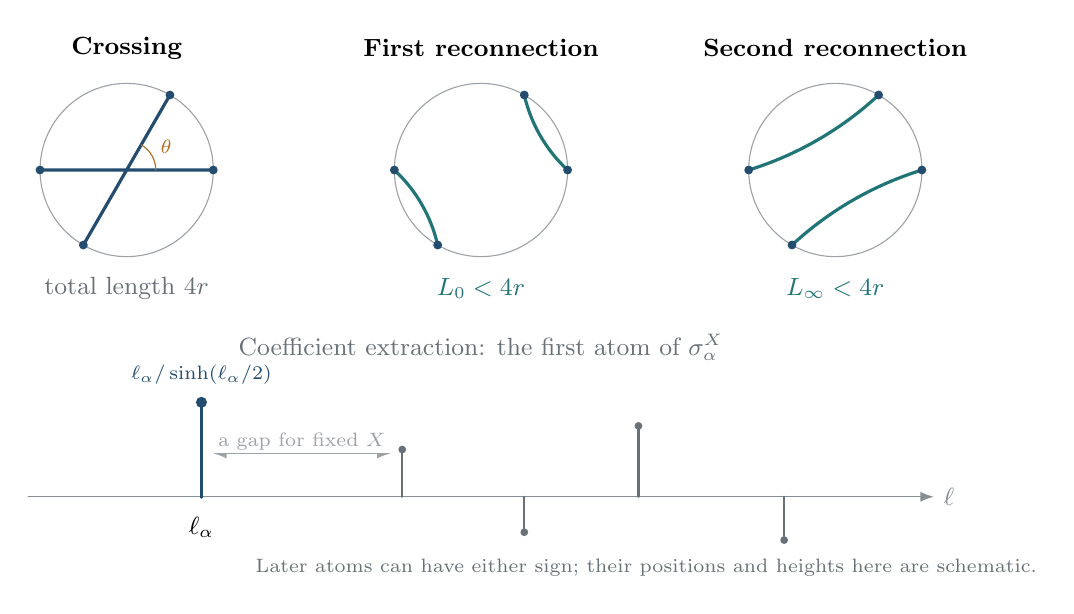
\begin{tikzpicture}[font=\small,>=Latex,line cap=round]
\begin{scope}[shift={(-4.5,1.6)}]
\draw[mpgray!65] (0,0) circle (1.1);
\node[font=\bfseries\small] at (0,1.55) {Crossing};
\draw[mpblue,line width=1.15pt] (0:1.1)--(180:1.1) (60:1.1)--(240:1.1);
\draw[mpochre] (.37,0) arc (0:60:.37);
\node[text=mpochre,font=\scriptsize] at (30:.58) {$\theta$};
\node[text=mpgray] at (0,-1.5) {total length $4r$};
\fill[mpblue] (0:1.1) circle (1.6pt);
\fill[mpblue] (60:1.1) circle (1.6pt);
\fill[mpblue] (180:1.1) circle (1.6pt);
\fill[mpblue] (240:1.1) circle (1.6pt);
\end{scope}
\begin{scope}[shift={(0,1.6)}]
\draw[mpgray!65] (0,0) circle (1.1);
\node[font=\bfseries\small] at (0,1.55) {First reconnection};
\draw[mpteal,line width=1.15pt] (1.10000000,0.00000000) arc[start angle=-132.84678884,delta angle=-34.30642232,radius=1.86486286];
\draw[mpteal,line width=1.15pt] (-1.10000000,0.00000000) arc[start angle=47.15321116,delta angle=-34.30642232,radius=1.86486286];
\node[text=mpteal] at (0,-1.5) {$L_0<4r$};
\fill[mpblue] (0:1.1) circle (1.6pt);
\fill[mpblue] (60:1.1) circle (1.6pt);
\fill[mpblue] (180:1.1) circle (1.6pt);
\fill[mpblue] (240:1.1) circle (1.6pt);
\end{scope}
\begin{scope}[shift={(4.5,1.6)}]
\draw[mpgray!65] (0,0) circle (1.1);
\node[font=\bfseries\small] at (0,1.55) {Second reconnection};
\draw[mpteal,line width=1.15pt] (1.10000000,0.00000000) arc[start angle=107.18035662,delta angle=25.63928676,radius=4.29338334];
\draw[mpteal,line width=1.15pt] (0.55000000,0.95262794) arc[start angle=-47.18035662,delta angle=-25.63928676,radius=4.29338334];
\node[text=mpteal] at (0,-1.5) {$L_\infty<4r$};
\fill[mpblue] (0:1.1) circle (1.6pt);
\fill[mpblue] (60:1.1) circle (1.6pt);
\fill[mpblue] (180:1.1) circle (1.6pt);
\fill[mpblue] (240:1.1) circle (1.6pt);
\end{scope}
  \draw[->,mpgray!80] (-5.75,-2.55)--(5.75,-2.55) node[right] {$\ell$};
  \node[text=mpgray] at (0,-.65) {Coefficient extraction: the first atom of $\sigma_\alpha^X$};
  \draw[mpblue,line width=1.4pt] (-3.55,-2.55)--(-3.55,-1.35);
  \fill[mpblue] (-3.55,-1.35) circle (2pt);
  \node[above=3pt,text=mpblue,font=\scriptsize] at (-3.55,-1.35)
    {$\ell_\alpha/\sinh(\ell_\alpha/2)$};
  \node[below=4pt] at (-3.55,-2.55) {$\ell_\alpha$};
  \foreach \x/\y in {-1.0/-.6,.55/.45,2.0/-.9,3.85/.55} {
    \draw[mpgray,line width=.8pt] (\x,-2.55)--(\x,{-2.55-\y});
    \fill[mpgray] (\x,{-2.55-\y}) circle (1.4pt);
  }
  \draw[<->,mpgray!65] (-3.4,-2.0)--node[above,font=\scriptsize,fill=white,inner sep=1pt]
    {a gap for fixed $X$}(-1.15,-2.0);
  \node[align=center,font=\scriptsize,text=mpgray] at (2.1,-3.45)
    {Later atoms can have either sign; their positions and heights here are schematic.};
\end{tikzpicture}
\caption[Crossing resolution and the first coefficient atom]{Reconnection and coefficient extraction are different operations.
The upper pictures show the two noncrossing pairings in a hyperbolic
metric disk; both shorten the original pair of diameters. Reconnection
changes connectivity and is not a negative direction of the length
Hessian within the original loop space. For a simple primitive support
$\alpha$, the lower schematic records the exact first atom of
$\sigma_\alpha^X$ at $\ell_\alpha$, with the stated mass; all remaining
atoms lie strictly above that length. Their depicted positions and
weights are illustrative, not numerical data.}
\label{fig:mono-reconnection-atoms}
\end{figure}
% END INLINE FIGURE

\subsection{An exponential coefficient bound from bracelet positivity}

The passage from compactly supported tests to heat kernels needs a
growth estimate. A direct crossing count gives an exponential in
$\ell_\gamma^2$ and only a small-time conclusion. Bracelet
positivity gives a stronger estimate.

At skein parameter $+1$, Dylan Thurston proves that every diagram
has a sign-coherent expansion in the bracelet
basis~\cite[Theorem 2]{DThurstonPositive}. A bracelet supported on
a simple curve $\beta$ with winding $n$ is the Chebyshev element
$P_n(z_\beta)$~\cite[Proposition 4.4]{DThurstonPositive}.
Distinct bracelet support curves are disjoint; their windings are
included in the length $\ell_X(D)=\sum_i n_i\ell_X(\beta_i)$.
The canonical twisted Fuchsian evaluation associated to $X$ is
positive on bracelet basis elements:
\[
 B_D(X)=\prod_i2\cosh\bigl(n_i\ell_X(\beta_i)/2\bigr)>0.
\]
For a one-component diagram representing $\gamma$, its evaluation
has absolute value $2\cosh(\ell_X(\gamma)/2)$. Sign coherence
therefore gives
\begin{equation}
 \sum_D |b_D(\gamma)| B_D(X)
 =2\cosh\bigl(\ell_X(\gamma)/2\bigr).
 \label{eq:coeffbraceletpositive}
\end{equation}
A spin structure identifies the $+1$ and $-1$ skein algebras by
signs on diagrams. Changing to~\eqref{eq:coeffbasis} also changes
only basis signs. On a simple generator this replaces $z_\beta$ by
$\epsilon_\beta T_\beta$, with $\epsilon_\beta\in\{1,-1\}$;
the identity $P_n(\epsilon x)=\epsilon^nP_n(x)$ shows that the
bracelet-to-multicurve coefficient magnitudes are unchanged.
All the absolute estimates below are consequently
valid in our unnegated trace basis. The positive Fuchsian evaluation
is an auxiliary algebraic estimate; the Laplacians defining
$\sigma_C^X$ still use unitary twists.

\begin{proposition}[Fixed-coefficient bound]
\label{prop:coeffgrowth}
Write $C=\sum_{j=1}^q r_j\beta_j$ with distinct support curves.
For $r\geq1$ and $\ell>0$ put
\[
 M_r(\ell)=\sup_{n\geq1}
 \frac{|[x^r]P_n(x)|}{2\cosh(n\ell/2)},\qquad
 K_{C,X}=\prod_{j=1}^q M_{r_j}(\ell_X(\beta_j)).
\]
Set $K_{\varnothing,X}=1$. These constants are finite, and
\begin{equation}
 \boxed{
 |a_C(\gamma)|\leq
 K_{C,X}\,2\cosh\bigl(\ell_X(\gamma)/2\bigr)
 }
 \label{eq:coeffexponentialbound}
\end{equation}
for every nontrivial closed curve, including iterates.
\end{proposition}

\begin{proof}
When $n\geq r\geq1$ have the same parity,
\[
 |[x^r]P_n(x)|
 =\frac{2n}{n+r}\binom{(n+r)/2}{r}
 \leq\frac{2n^r}{r!};
\]
otherwise the coefficient is zero. Consequently
\begin{equation}
 M_r(\ell)\leq
 \frac{2}{r!}\left(\frac{2r}{e\ell}\right)^r<\infty.
 \label{eq:coeffMrbound}
\end{equation}
To contribute to $C$, a bracelet element must contain every
$\beta_j$ in its support. Additional support curves must contribute
constant terms, which are either zero or $\pm2$. Their absolute
constant coefficient divided by $2\cosh(n\ell/2)$ is at most one.
It follows that
\[
 |[T_C]B_D|\leq K_{C,X}B_D(X).
\]
Apply this bound to~\eqref{eq:coeffbraceletpositive} and use the
triangle inequality. Spin and basis signs do not affect the estimate.
\end{proof}

For a single simple $\alpha$ one can use
\[
 K_{\alpha,X}
 =\sup_{\substack{n\geq1\\n\text{ odd}}}
   \frac{n}{2\cosh(n\ell_\alpha/2)}
 \leq\frac{2}{e\ell_\alpha}.
\]
The estimates are uniform for a fixed target $C$ on compact subsets
of Teichm\"uller space. Related positivity and Chebyshev estimates
for analytic lamination expansions on punctured planar surfaces
appear in Basok--Chelkak~\cite[Section 4.4, Theorems 4.7 and 4.9]{BasokChelkak}. Their
full analytic expansion theorem is not needed here.

\begin{corollary}[Growth of the signed measure]
\label{cor:coeffmeasuregrowth}
For each fixed $X,C$ there is a constant $B_{C,X}$ such that
\begin{equation}
 |\sigma_C^X|([0,R])\leq B_{C,X}(1+R)e^R.
 \label{eq:coeffmeasuregrowth}
\end{equation}
\end{corollary}

\begin{proof}
Put $\varepsilon=\operatorname{sys}(X)>0$ and
$L=k\ell_\delta$. Each orbital summand has absolute mass at most
\[
 \frac{\ell_\delta}{\sinh(L/2)}
 K_{C,X}2\cosh(L/2)
 \leq2K_{C,X}\coth(\varepsilon/2)L.
\]
The number of primitive/iterate classes of length at most $R$ is
$O_X(e^R)$. One elementary proof conjugates each class so its axis
passes a bounded distance from a fixed point in $\HH^2$; the chosen
element then moves that point by at most $R+O_X(1)$. Orbit points
are uniformly separated, and hyperbolic disk area is $O(e^R)$.
Summing the displayed mass bound proves the claim. No prime-geodesic
asymptotic is required.
\end{proof}

\subsection{Convergent heat and Laplace transforms}

Define
\begin{align}
 G_C^X(t)&=\int_0^\infty e^{-L^2/(4t)}\,\dd\sigma_C^X(L),
 &H_C^X(t)&=\frac{e^{-t/4}}{\sqrt{4\pi t}}G_C^X(t),
 \label{eq:coeffheatdefinition}\\
 D_C^X(s)&=\int_0^\infty e^{-sL}\,\dd\sigma_C^X(L).
 &&\label{eq:coeffLaplacedefinition}
\end{align}
By~\eqref{eq:coeffmeasuregrowth}, $G_C$ and $H_C$ are absolutely
convergent for every $t>0$, and holomorphic for $\Re t>0$ with
the principal square root. The Laplace transform is absolutely
convergent and holomorphic for $\Re s>1$. Differentiation in these
variables is permitted locally uniformly in the stated domains.

There is also a convergent expansion of the whole heat trace.
For a finite character polynomial set
\[
 \|f\|_2=\sum_C|[T_C]f|\,2^{\#C},\qquad
 c_X=\frac{\log(1+\sqrt2)}{\operatorname{sys}(X)}.
\]
The subscript $2$ denotes the trace bound $|\tr\rho(\alpha)|\leq2$;
this is a weighted coefficient norm, not an $L^2$ norm.
The Chebyshev recurrence gives
\[
 \sum_r|[x^r]P_n(x)|2^r\leq2(1+\sqrt2)^n.
\]
A bracelet has at most $3g-3$ distinct support curves, so
$\|B_D\|_2\leq2^{3g-3}e^{c_X\ell_X(D)}$.
In~\eqref{eq:coeffbraceletpositive} the nonzero coefficients are
integers, and $B_D(X)\geq e^{\ell_X(D)/2}$. Hence
$\ell_X(D)\leq\ell_X(\gamma)+2\log2$ for every occurring $D$,
and $\sum_D|b_D|\leq2e^{\ell_X(\gamma)/2}$. Therefore
\begin{equation}
 \|\tr_\gamma\|_2\leq
 C_X e^{(1/2+c_X)\ell_X(\gamma)},\qquad
 C_X=2^{3g-2}e^{2c_X\log2}.
 \label{eq:coeffallchannelbound}
\end{equation}
Gaussian decay dominates this exponential bound and the orbit count.
It follows that
\begin{equation}
 \boxed{
 \operatorname{Tr}e^{-t\Delta_\rho}-2I_X(t)
 =\sum_{C\in\mathscr C(S)}H_C^X(t)T_C(\rho),\qquad t>0,
 }
 \label{eq:coefffullheatexpansion}
\end{equation}
where
\[
 I_X(t)=\frac{\operatorname{Area}(X)}{4\pi}
  \int_\RR r\tanh(\pi r)e^{-t(r^2+1/4)}\,\dd r,
 \qquad \sum_C|H_C^X(t)|2^{\#C}<\infty.
\]
The series is uniform on the unitary character variety and locally
uniform for $\Re t>0$. It is obtained by taking the limit of the
finite length-cutoff expansions; the preceding absolute estimate
justifies the rearrangement. For a compact set of such $t$,
$\Re(1/t)$ has a positive lower bound, so the same Gaussian
majorant proves local uniformity and termwise holomorphy. On the
spectral side, smooth cutoffs of the Gaussian converge in the
Schwartz topology on the real spectral axis and at the finitely
many imaginary spectral parameters; the compact-surface Weyl bound
justifies passing to the heat trace for each unitary twist.

This construction does not assert uniqueness among arbitrary
infinite expansions of a continuous function. For example,
$\|\tr\rho(\alpha^{2n+1})\|_\infty\leq2$, while its
$T_\alpha$ coefficient is $(-1)^n(2n+1)$. Coefficient extraction
is therefore not bounded for the uniform norm on unitary characters.
Our coefficients are fixed by the finite spectral tests first;
the estimates then justify their heat transform.

\begin{proposition}[Simple-curve semiclassical term]
\label{prop:coeffheatfirst}
Let $\alpha$ be simple and $\ell=\ell_X(\alpha)$. Choose
$b>\ell$ so that every other orbital contribution to
$\sigma_\alpha^X$ has length at least $b$. Then
\begin{align}
 G_\alpha^X(t)
 &=\frac{\ell}{\sinh(\ell/2)}e^{-\ell^2/(4t)}
   +O\bigl(e^{-b^2/(4t)}\bigr),\notag\\
 H_\alpha^X(t)
 &=\frac{e^{-t/4}}{\sqrt{4\pi t}}
   \frac{\ell}{\sinh(\ell/2)}e^{-\ell^2/(4t)}
   \left[1+O\!\left(e^{-(b^2-\ell^2)/(4t)}\right)\right],
 \label{eq:coeffheatfirst}\\
 D_\alpha^X(s)
 &=\frac{\ell}{\sinh(\ell/2)}e^{-s\ell}
   \left[1+O\bigl(e^{-s(b-\ell)}\bigr)\right]
   \quad(s\to+\infty).
 \label{eq:coeffLaplacefirst}
\end{align}
In particular,
\begin{equation}
 \boxed{
 \ell^2=-\lim_{t\downarrow0}4t\log G_\alpha^X(t),\qquad
 \ell=-\lim_{s\to+\infty}s^{-1}\log D_\alpha^X(s).
 }
 \label{eq:coefflengthlimits}
\end{equation}
Both logarithms are real for sufficiently small $t$, respectively
sufficiently large positive $s$.
\end{proposition}

\begin{proof}
Separate the first atom in~\eqref{eq:coefffirstatom}. For its
remaining measure $\tau$, supported on $[b,\infty)$, fix $t_0>0$.
For $0<t\leq t_0$,
\[
 \int e^{-L^2/(4t)}\,\dd|\tau|(L)
 \leq e^{-b^2/(4t)+b^2/(4t_0)}
       \int e^{-L^2/(4t_0)}\,\dd|\tau|(L).
\]
The last integral is finite. The same argument with a fixed real
$s_0>1$ gives the Laplace remainder. The leading masses are
positive, so the leading terms eventually dominate the signed tails.
\end{proof}

After removing the explicit $e^{-t/4}$ factor, the correction to
the single-geodesic term is exponentially small, rather than a new
power series in $t$. Thus the constant-curvature heat coefficient
has an exact isolated-orbit prefactor, followed by contributions at
larger length actions. For $m\alpha$ replace the action by
$(m\ell_\alpha)^2/(4t)$ and the mass by
$\ell_\alpha/\sinh(m\ell_\alpha/2)$.

\subsection{All iterates of a simple curve}

Write $\sigma_C^{X,[\delta]}$ for the contribution of one primitive
unoriented class $\delta$ and all of its iterates. The polynomial
identity
\begin{equation}
 P_k(x)=\sum_{j=0}^{\lfloor k/2\rfloor}
 (-1)^j\frac{k(k-j-1)!}{j!(k-2j)!}x^{k-2j},\qquad k\geq1,
 \label{eq:coeffChebyshev}
\end{equation}
follows from the recurrence. If $\alpha$ is simple, the coefficient
of $m\alpha$ vanishes unless $k=m+2j$, and for $m\geq1$ is
\begin{equation}
 b_{m+2j,m}=(-1)^j
  \frac{(m+2j)(m+j-1)!}{j!\,m!}.
 \label{eq:coeffsimplepowers}
\end{equation}
In particular, with $\ell=\ell_\alpha$,
\begin{equation}
 \boxed{
 \sigma_\alpha^{X,[\alpha]}
 =\ell\sum_{j\geq0}
   \frac{(-1)^j(2j+1)}{\sinh((2j+1)\ell/2)}
   \delta_{(2j+1)\ell}.
 }
 \label{eq:coeffoddpowers}
\end{equation}
The first masses have multipliers $1,-3,5,-7,\ldots$ at
$\ell,3\ell,5\ell,7\ell,\ldots$. For $2\alpha$ the multipliers
are $1,-4,9,-16,\ldots$ at $2\ell,4\ell,6\ell,8\ell,\ldots$.
These are explicit later atoms, not changes to the first-atom mass.

For $m\geq1$ the coefficient generating function is
\begin{equation}
 B_m(q):=\sum_{k\geq1}b_{k,m}q^k
 =\frac{q^m(1-q^2)}{(1+q^2)^{m+1}}.
 \label{eq:coeffpowergenerating}
\end{equation}
Indeed,
$\sum_{k\geq1}P_k(x)q^k=(xq-2q^2)/(1-xq+q^2)$,
and extracting $x^m$ gives this formula. Expanding the hyperbolic
denominator yields, for $\Re s>-1/2$,
\begin{align}
 D_{m\alpha}^{X,[\alpha]}(s)
 &=2\ell\sum_{n\geq0}B_m(q_n),
 &q_n&=e^{-(s+n+1/2)\ell},\notag\\
 &=2^{1-m}\ell\sum_{n\geq0}
   \sech^m(u_n)\tanh(u_n),
 &u_n&=(s+n+1/2)\ell.
 \label{eq:coeffpowerLaplace}
\end{align}
This larger convergence domain concerns the one fixed primitive
family; the proved half-plane for the full $D_C$ is $\Re s>1$.

The heat contribution of the same family is
\begin{align}
 H_\alpha^{X,[\alpha]}(t)
 ={}&\frac{e^{-t/4}}{\sqrt{4\pi t}}
 \frac{\ell e^{-\ell^2/(4t)}}{\sinh(\ell/2)}\notag\\
 &\mathrel{}\times\left[
 1-3\frac{\sinh(\ell/2)}{\sinh(3\ell/2)}e^{-2\ell^2/t}
 +5\frac{\sinh(\ell/2)}{\sinh(5\ell/2)}e^{-6\ell^2/t}
 -\cdots\right].
 \label{eq:coeffpowerheat}
\end{align}
Other primitive classes may supply corrections before these particular
iterate actions. Once $\ell_\alpha$ is recovered, subtracting the
$j\geq1$ terms of~\eqref{eq:coeffoddpowers} removes exactly the
nonprimitive powers of the simple curve $\alpha$; it leaves powers
of nonsimple curves that resolve with an $\alpha$ coefficient.

\subsection{A figure-eight family and an exact cancellation}

Take an embedded geodesic pair of pants with three distinct essential
cuffs $a,b,c$, and $c=(ab)^{-1}$. Set
\[
 x=T_a,\qquad y=T_b,\qquad z=T_c,\qquad
 \gamma=a^{-1}b,
 \qquad T_\gamma=xy-z.
\]
These are functions of arbitrary unitary holonomy. The minus sign
therefore differs from the positive hyperbolic length convention
in~\eqref{eq:figuretrace}. Powers are given exactly by
$T_{\gamma^k}=P_k(xy-z)$. For example,
\begin{align*}
 T_\gamma&=xy-z,\\
 T_{\gamma^2}&=x^2y^2-2xyz+z^2-2,\\
 T_{\gamma^3}&=x^3y^3-3x^2y^2z+3xyz^2-z^3-3xy+3z.
\end{align*}
Only multicurves $C=ra+rb+mc$ occur. Put $d=r+m\geq1$.
Their coefficients vanish unless $k=d+2j$, and in that case
\begin{equation}
 \boxed{
 a_{ra+rb+mc}(\gamma^k)
 =(-1)^{j+m}\frac{k(k-j-1)!}{j!\,r!\,m!}
 =(-1)^m\binom{r+m}{r}b_{k,r+m}.
 }
 \label{eq:coefffigurepowers}
\end{equation}
This follows by substituting $xy-z$ into~\eqref{eq:coeffChebyshev}
and expanding the relevant monomial. Consequently
\[
 \sum_{k\geq1}a_{ra+rb+mc}(\gamma^k)q^k
 =(-1)^m\binom{r+m}{r}
 \frac{q^{r+m}(1-q^2)}{(1+q^2)^{r+m+1}}.
\]

For $r+m=1$ the two target coefficients are opposite for every
iterate. If $L=\ell_\gamma$, then
\begin{equation}
 \boxed{
 \sigma_{a+b}^{X,[\gamma]}
 =-\sigma_c^{X,[\gamma]}
 =L\sum_{j\geq0}
 \frac{(-1)^j(2j+1)}{\sinh((2j+1)L/2)}
 \delta_{(2j+1)L}.
 }
 \label{eq:coefffigurecancellation}
\end{equation}
Thus $\sigma_c^X+\sigma_{a+b}^X$ cancels the entire chosen
figure-eight family, including all its powers. This does not assert
that the full sum vanishes: other primitive classes contribute to
both coefficients. It gives an exact family-by-family cancellation
which is preserved by either transform in
\eqref{eq:coeffheatdefinition}--\eqref{eq:coeffLaplacedefinition}.

The distinct-cuff assumption makes the monomials above distinct
multicurve basis elements. If cuff images coincide, as in some
one-holed-torus configurations of Section~\ref{sec:figures}, the
corresponding variables must first be identified and equal basis
terms collected; the displayed coefficient indexing cannot be
carried over unchanged.

\subsection{Metric variation and the twist derivative}

For a fixed topological $C$, the map
$X\mapsto\sigma_C^X$ is smooth as a distribution-valued map.
After applying any compactly supported test function, it is locally
a finite sum of smooth length functions. It is not asserted to be
real analytic for arbitrary smooth test functions.

For an orbital label $(\delta,k)$ write
\[
 L=k\ell_\delta,\qquad
 w=\ell_\delta\operatorname{csch}(L/2).
\]
For a tangent vector $v$ to Teichm\"uller space one has
\begin{equation}
 D_v\sigma_C^X
 =\sum_{\delta,k}a_C(\delta^k)
  \left[(D_vw)\delta_L-w(D_vL)\delta'_L\right],
 \label{eq:coeffmetricvariation}
\end{equation}
where $\langle\delta'_L,\varphi\rangle=-\varphi'(L)$ and
\[
 D_vL=kD_v\ell_\delta,\qquad
 D_vw=\operatorname{csch}(L/2)
       \left(1-\frac L2\coth\frac L2\right)D_v\ell_\delta.
\]
The coefficients $a_C$ are constant under metric variation. This
formula describes movement of the atoms as well as variation of
their masses; omitting the $\delta'_L$ term would lose the length
variation itself.

For a twist of displacement $\tau_\beta$ about a simple geodesic
$\beta$, Wolpert's cosine formula gives
\begin{equation}
 \frac{\partial\ell_\delta}{\partial\tau_\beta}
 =\sum_{p\in\delta\cap\beta}\cos\theta_p,
 \label{eq:coeffWolpert}
\end{equation}
with the consistent right-twist angle convention and intersections
counted with multiplicity~\cite{WolpertTwist}. Substitution in
\eqref{eq:coeffmetricvariation} gives an exact variation formula
for every coefficient distribution. For a simple $\alpha$, one
can equivalently differentiate the localized ratio
\eqref{eq:coeffmomentratio}; it recovers~\eqref{eq:coeffWolpert}
from two spectral coefficient moments, without an infinite limit.
The first-variation argument also applies when $\delta$ is immersed:
cut it at its crossings with $\beta$. Interior variations of the
geodesic arcs cancel by stationarity; the relative tangential
displacement at each paired endpoint contributes the projection
$\cos\theta_p$. Summing over the passages through the cut gives
the formula with precisely the stated multiplicities. If $\delta$
is a power of $\beta$, its twist derivative is zero and the sum is
interpreted as empty.

The compact-set gap in Proposition~\ref{prop:coefffirstatom} also
permits differentiating the leading heat asymptotic locally.
The leading logarithmic response is
\begin{equation}
 D_v\log H_\alpha^X(t)
 =\left[-\frac{\ell_\alpha}{2t}
          +\frac1{\ell_\alpha}
          -\frac12\coth\frac{\ell_\alpha}{2}\right]
    D_v\ell_\alpha
  +O\bigl(t^{-1}e^{-c/t}\bigr)
 \label{eq:coeffheatvariation}
\end{equation}
for some local $c>0$. To justify the differentiated tail, metric
length derivatives on a compact parameter neighborhood are bounded
by constants times the length, while
\eqref{eq:coeffexponentialbound} is locally uniform. Gaussian
decay absorbs the additional polynomial factors.

\subsection{The logarithmic product and primitive extraction}

A useful connection to the Selberg product keeps the orientation
normalization explicit. Define, for $\Re v>1$,
\begin{equation}
 \mathcal Z_\rho^X(v)
 =\prod_{\delta\in\mathcal P_{\rm un}}\prod_{n\geq0}
 \det\left(I-e^{-(v+n)\ell_\delta}\rho(\delta)\right).
 \label{eq:coeffunorientedproduct}
\end{equation}
This definition uses unoriented primitives; a product over both
oriented conjugacy classes squares it. Expanding the logarithm gives
\begin{equation}
 2\left.\frac{\partial}{\partial v}
     \log\mathcal Z_\rho^X(v)\right|_{v=s+1/2}
 =\sum_{\delta,k}
   \frac{\ell_\delta e^{-sk\ell_\delta}}
        {\sinh(k\ell_\delta/2)}\tr\rho(\delta^k).
 \label{eq:coeffproductderivative}
\end{equation}
With coefficients defined by finite length cutoffs, the $T_C$
coefficient on the right is $D_C^X(s)$ for $\Re s>1$.
The coefficient estimate proves this assertion; it is not an
appeal to continuity of coefficient extraction in the uniform norm.
No meromorphic continuation of the individual $D_C$ is established
by this calculation.

Removing all iterates by a global Chebyshev substitution is not
legitimate in the rank-two character ring. If
$x=\tr A$, $y=\tr B$, $u=\tr(AB)$, and $v=\tr(AB^{-1})$,
then $u+v=xy$, but
\begin{equation}
 P_2(u)+P_2(v)-P_2(x)P_2(y)
 =2\bigl(\tr[A,B]-2\bigr),
 \label{eq:coeffAdamsobstruction}
\end{equation}
which is generally nonzero. Thus sending every trace to its
Chebyshev polynomial does not define a multiplicative operation
on this character ring.

There is an exact repair if extra twisting data are supplied.
For the original $\mathrm{SU}(2)$ representation $\rho$, work in
the virtual representation ring generated by its symmetric powers.
Let $\psi^k\rho$ denote its Adams operation, characterized by
$\chi_{\psi^k\rho}(\gamma)=\chi_\rho(\gamma^k)$. For the
standard rank-two representation,
\[
 \psi^k\rho=\operatorname{Sym}^k\rho-
             \operatorname{Sym}^{k-2}\rho\quad(k\geq2),
 \qquad \psi^1\rho=\rho.
\]
Trace formulas extend additively to virtual representations.
All twists used here have inverse-invariant characters, so the
unoriented normalization is preserved. Let $\Sigma_\rho$ denote the character-valued geometric measure
on the right of~\eqref{eq:coefftwistedSelberg}, and set
\[
 Q_\rho=\sinh(L/2)\Sigma_\rho,\qquad
 P_\rho=\sum_{\delta\in\mathcal P_{\rm un}}
         \ell_\delta\chi_\rho(\delta)\delta_{\ell_\delta}.
\]
For $D_k\delta_L=\delta_{kL}$,
\[
 Q_\rho=\sum_{k\geq1}D_kP_{\psi^k\rho},\qquad
 \boxed{P_\rho=\sum_{k\geq1}\mu(k)D_kQ_{\psi^k\rho}.}
\]
These sums are locally finite, and the second identity follows from
$\psi^j\psi^k=\psi^{jk}$ and divisor M\"obius inversion. It requires
spectra for higher symmetric-power twists, which are additional
data beyond the original rank-two family. The explicit subtraction
in~\eqref{eq:coeffoddpowers} needs no such enlargement.

\subsection{Scope and further questions}

The construction now supplies signed coefficient distributions,
an isolated first simple-curve atom, globally convergent heat
transforms, a Laplace half-plane, explicit iterate families, a
figure-eight cancellation, and metric derivatives. It has not
produced a positive measure with the weights of simple-geodesic
counting, nor a pointwise constant McShane series.

The scalar limitation is genuine: length-isospectral closed
hyperbolic surfaces can have different simple length spectra
\cite{AougabLahnLovingMiller}. The labelled holonomy family retains
the information used by~\eqref{eq:coeffmomentratio}.

For a counting comparison, let $d=6g-6$ and normalize Thurston
measure by the integral multicurve lattice. If
\[
 B(X)=\mu_{\rm Th}\{\lambda:\ell_X(\lambda)\leq1\},
\]
ordinary lattice counting gives
$\#\{C\in\mathcal{ML}_{\ZZ}:\ell_X(C)\leq R\}\sim B(X)R^d$
\cite[Proposition 3.1]{MirzSimple}. Its Laplace consequence is
\[
 \sum_{C\in\mathcal{ML}_{\ZZ}}e^{-t\ell_X(C)}
 \sim\Gamma(d+1)B(X)t^{-d}\qquad(t\downarrow0).
\]
This is a target for a measure comparison, not a consequence of
the coefficient heat expansion. It counts all weighted multicurves;
connected or fixed-orbit counts require additional information.
The large-length limit here is also different from the
minimum-selection limits in~\eqref{eq:coefflengthlimits}.

Two concrete further problems are to continue $D_C(s)$ beyond its
proved half-plane, with control of the coefficient operation, and
to find combinations of coefficients whose cancellations organize
globally over pants. Formula~\eqref{eq:coefffigurecancellation}
provides an exact local model for the second problem. An identity
constant in $X$ would require an additional normalization or
geometric partition; the existence of these transforms alone does
not supply that constancy. Section~\ref{sec:quantitativecounting}
strengthens the lattice benchmark and gives explicit orbital gaps,
uniform recovery estimates, and a conditional counting criterion.


\clearpage

\section{Quantitative counting and coefficient cancellation}
\label{sec:quantitativecounting}

The preceding construction raises a quantitative question: can explicit
crossing resolutions give a counting remainder with a specified exponent
and geometric constants? We first give an elementary counting benchmark.
We then prove a systole-dependent gap and a uniform recovery estimate,
and show on a fixed surface why their exponential separation scale is
unavoidable for estimates of individual orbital terms. Finally, a finite
support coefficient and a smoothing criterion isolate the additional
estimate needed for connected-curve counting.

\subsection{Effective counting and the meaning of an explicit saving}
\label{subsec:countknown}

Continue with a closed hyperbolic surface $X$ of genus $g\geq2$, and
put $d=6g-6$.  For a fixed nonzero rational multicurve $\gamma_0$, write
\[
 N_{X,\gamma_0}(R)=
 \#\{\gamma\in\operatorname{Mod}(S)\gamma_0:
                         \ell_X(\gamma)\leq R\}.
\]
A remainder $O(R^{d-\kappa})$ with $\kappa>0$ is called a
power saving because it is smaller than the $R^d$ main term
by a factor $R^{-\kappa}$. The subscript on $O_{X,\gamma_0}$
allows its constant to depend on the metric and curve type.
An existence theorem for a positive $\kappa$ and an explicit
numerical value for it are different levels of quantitative information.

Eskin--Mirzakhani--Mohammadi prove that there exists
$\kappa(g)>0$ such that
\begin{equation}
 N_{X,\gamma_0}(R)
 =c_{X,\gamma_0}R^d
   +O_{X,\gamma_0}(R^{d-\kappa(g)}).
 \label{eq:countEMM}
\end{equation}
Their theorem also allows variable negative curvature; the hyperbolic
case suffices here~\cite[Theorem 1.1]{EMMEffective}.  The theorem
states the existence of the exponent rather than a numerical value.
Its proof uses exponential mixing of the Teichm\"uller flow.  A
specified exponent and certified constants for a given surface would
therefore be additional quantitative information.  This distinction
does not diminish the proved power saving or establish that its
constants are intrinsically noncomputable.

The coefficient distributions offer explicit local formulas, but
their present estimates do not improve~\eqref{eq:countEMM}.
The task is to control a growing collection of connected supports.
The qualitative leading term, treated in
\cite{MirzSimple,RivinSimpleAsymptotics}, and an effective remainder
are separate questions.  It is useful first to record how much
quantitative control follows from ordinary lattice geometry alone.

\subsection{A constructive lattice benchmark for all multicurves}
\label{subsec:countlattice}

A measured lamination is a closed union of disjoint geodesic leaves
with a compatible transverse measure. Weighted disjoint closed
curves are its integral examples, and geometric length extends
continuously and homogeneously to this space. A train track is a
finite branched diagram carrying such leaves; nonnegative branch
weights satisfy switch equations expressing conservation at each
junction. These equations provide linear coordinate cones and
integral lattices. Thurston measure is the compatible Lebesgue
measure in those coordinates, with its lattice normalization fixed.

Let $\mathcal{ML}_{\ZZ}(S)$ denote integral measured laminations,
equivalently essential simple multicurves with positive integer
weights.  These include disconnected supports.  Normalize Thurston
measure by the actual integral-lamination lattice in each chart, and
set
\[
 M_X(R)=\#\{C\in\mathcal{ML}_{\ZZ}(S)\setminus\{0\}:
                  \ell_X(C)\leq R\},\qquad
 B(X)=\mu_{\mathrm{Th}}\{\lambda:\ell_X(\lambda)\leq1\}.
\]

\begin{proposition}[Total multicurve error]
\label{prop:countall}
For the fixed surface $X$,
\begin{equation}
 \boxed{M_X(R)=B(X)R^d+O_X(R^{d-1}).}
 \label{eq:countall}
\end{equation}
The error can be bounded using finitely many lattice covolumes,
fundamental-cell radii, convex-body inradii and volumes, and
lower-dimensional face bounds.
\end{proposition}

\begin{proof}
Here is the quantitative lattice estimate needed for the argument.
Let $\Lambda\subset\RR^d$ have covolume $v$ and a fundamental cell
$F\subset B(0,\rho)$.  Suppose the convex compact body $K$ has volume
$V$ and contains $B(x_0,r)$, where $r>0$.  Put $a=\rho/r$.  Then
\begin{equation}
 \frac Vv(R-a)_+^d
 \leq\#(\Lambda\cap RK)
 \leq\frac Vv(R+a)^d.
 \label{eq:countsandwich}
\end{equation}
Indeed, up to null sets the lattice cells tile Euclidean space, so
\[
 (RK)\ominus B_\rho
 \ \subset\!
 \bigcup_{p\in\Lambda\cap RK}(p+F)
 \ \subset RK+B_\rho.
\]
Here $A\ominus B_\rho=\{x:x+B_\rho\subset A\}$.
Writing $K_0=K-x_0$, we have $B_r\subset K_0$ and
\[
 RK+B_\rho\subset Rx_0+(R+a)K_0.
\]
For $R\geq a$, also
$Rx_0+(R-a)K_0\subset(RK)\ominus B_\rho$.
Taking volumes proves~\eqref{eq:countsandwich}; the lower bound is
zero when $R<a$.  Notice that the homotheties are centered at
$Rx_0$, since the origin can be a boundary point of $K$.
For $R\geq a$ this gives the explicit bound
\begin{equation}
 \left|\#(\Lambda\cap RK)-\frac VvR^d\right|
 \leq d\,2^{d-1}\frac Vv\frac\rho r\,R^{d-1}.
 \label{eq:countcellerror}
\end{equation}
The upper increment $(R+a)^d-R^d$ dominates the lower decrement.

The scale of the error is familiar from a square. For
$K=[0,1]^2$ and $\Lambda=\mathbb Z^2$, the exact count in
$RK$ is $(\lfloor R\rfloor+1)^2=R^2+O(R)$.
Interior lattice cells account for area; the uncertainty lies in
cells meeting the boundary, whose number has one lower power of
$R$. The inradius and cell-radius argument above supplies this
principle for a general convex body, without assuming a smooth boundary.
The covolume $v$ is the volume of one lattice fundamental cell.

To apply this estimate, use a finite rational polyhedral cone
subdivision subordinate to train-track charts, with their actual
integral weight lattices. Length is convex in each train-track cone,
by the surgery argument in \cite[Theorem 5.1]{EMMEffective}.
The finite polyhedral handling of chart overlaps is given in
\cite[Lemma 5.1 and the end of the proof of Theorem 1.1 in
Section 8]{EMMEffective}; a further finite subdivision makes the
chambers convex and their overlaps faces. In the coordinates of
each chamber $Q_i$, the sets
$K_i=Q_i\cap\{\ell_X\leq1\}$ are compact convex bodies.
Indeed, continuity and positivity of length on the projectivized
cone give boundedness, and scaling an interior point of a
full-dimensional chamber to length less than one gives an interior
ball. Lower-dimensional chambers are handled as faces. Apply
\eqref{eq:countsandwich} in every full-dimensional chamber with its
own integral lattice.  Their normalized volumes sum to $B(X)$.
In particular, a coordinate parity condition must be absorbed into
the lattice covolume, not silently discarded.

Shared faces can be assigned to one chamber.  Alternatively, count
closed chambers and bound the overcount.  If a face has dimension
$1\leq k\leq d-1$, its unit-length part lies in a ball of radius $A_F$, and
its induced lattice has shortest nonzero vector of length $\delta_F$,
disjoint-ball packing gives
\[
 \#(\Lambda_F\cap RK_F)
 \leq\left(1+\frac{2RA_F}{\delta_F}\right)^k.
\]
Zero-dimensional faces contribute at most one point each.  The
finite sum of these bounds is $O_X(R^{d-1})$.
Removing the zero multicurve changes the answer by one.
\end{proof}

This refines the elementary total-multicurve lattice asymptotic in
\cite[Proposition 3.1]{MirzSimple}; it is a benchmark for the new
machinery.  Formula~\eqref{eq:countcellerror} is explicit once bounds
on its geometric inputs are certified.  It does not supply numerical
values for an unspecified surface.  Fixed train-track representatives
give linear upper bounds for length, and coordinate length estimates
such as~\cite{LuoStongLengths} help certify the required geometric
bounds.  Hyperbolic length itself need not be piecewise linear.
For example, choose an interior rational weight vector in a chamber
and scale it until a certified linear upper bound for length is less
than one.  A small coordinate ball then remains both in that chamber
and below the upper bound, producing an inradius certificate.
For an outer-radius certificate one needs a lower bound for length
on the chamber's unit coordinate sphere.  A finite filling collection
of curves, together with collar inequalities and their
piecewise-linear intersection functions, supplies such a bound.
The constants can deteriorate when the surface degenerates; no
uniformity over the entire moduli space is being asserted.
On a fixed compact subset of Teichm\"uller space the same finite
coordinate construction and uniform length comparisons give uniform
versions of the bounds.

\subsection{Primitivity, connectivity, and the torus benchmark}
\label{subsec:countprimitive}

Write $C=\sum_jm_j\alpha_j$ with distinct simple supports.  Call $C$
primitive as an integral lamination if $\gcd_jm_j=1$.
Every nonzero integral multicurve is uniquely $kC_0$ with $C_0$
primitive.  This intrinsic definition avoids coordinate conventions:
division by $k$ is allowed precisely when the resulting lamination
remains integral.  Let $P_X(R)$ count these primitive laminations.
M\"obius inversion gives
\[
 P_X(R)=\sum_{k\leq R/\operatorname{sys}(X)}\mu(k)M_X(R/k).
\]
Since $d>2$, the error series $\sum k^{-(d-1)}$ converges, while
the truncated leading-term tail is $O_X(R)$.  Therefore
\begin{equation}
 P_X(R)=\frac{B(X)}{\zeta(d)}R^d+O_X(R^{d-1}).
 \label{eq:countprimitive}
\end{equation}
Here $\zeta(d)=\sum_{k\ge1}k^{-d}$, and the arithmetic
M\"obius function is the one defined in Section~\ref{sec:coefficientdistributions}.
For example, $2\alpha+3\beta$ is primitive when $\alpha,\beta$
are distinct disjoint simple supports, since $\gcd(2,3)=1$.
It still has two supports. Dividing out a common integer weight
and requiring connected support answer different questions.

A union $\alpha+\beta$ of distinct disjoint simple curves is primitive
but disconnected.  Thus~\eqref{eq:countprimitive} does not count
connected simple curves in higher genus.

For a once-punctured torus every essential multicurve has one
distinct support.  The McShane--Rivin norm on $H_1(T;\RR)$ identifies
simple curves with primitive lattice vectors modulo sign.  If $B_X$
is its full centrally symmetric unit ball, our unoriented convention
gives
\begin{equation}
 N_X(R)=\frac{\operatorname{area}(B_X)}{2\zeta(2)}R^2
                  +O_X(R\log R).
 \label{eq:counttorus}
\end{equation}
This is the norm-and-M\"obius-inversion argument of
\cite[Theorem 4.1]{McShaneRivinTori}; the factor $1/2$ identifies
opposite homology vectors.  The logarithm comes from
$\sum_{k\leq O_X(R)}k^{-1}$.  This independent torus benchmark does
not extend the closed-surface trace formula across a cusp.


\subsection{A fixed-surface obstruction to uniform first-atom separation}
\label{subsec:countnearcollision}

The exponentially small remainder for one fixed simple curve does not
remain small uniformly over curves whose length tends to infinity.
There is an explicit obstruction on a fixed hyperbolic surface, with
no degeneration of its metric.

\begin{proposition}[An exponentially close pants contribution]
\label{prop:countnearcollision}
On every closed hyperbolic surface $X$ of genus at least two there
are fixed distinct simple curves $a,b$, and simple curves $c_n$
with $R_n=\ell_X(c_n)\to\infty$, such that $a,b,c_n$ bound
embedded geodesic pairs of pants. Let $\gamma_n$ be their
figure-eight curves with
$T_{\gamma_n}=T_aT_b-T_{c_n}$, and set
\[
 A=\cosh\frac{\ell_X(a)}2\cosh\frac{\ell_X(b)}2,
 \qquad L_n=\ell_X(\gamma_n).
\]
Then
\begin{align}
 L_n-R_n&=8A e^{-R_n/2}+O(e^{-R_n}),\notag\\
 L_n^2-R_n^2&=16A R_n e^{-R_n/2}
                    +O(R_n e^{-R_n}).
 \label{eq:countpantsgap}
\end{align}
The coefficient of $T_{c_n}$ in $T_{\gamma_n}$ is $-1$.
\end{proposition}

\begin{proof}
Choose distinct disjoint nonseparating curves $a,b$ whose complement
after cutting is connected, of genus $g-2$ with four boundary
components. In this cut surface let $c$ bound a pair of pants with
one copy of $a$ and one copy of $b$. Choose an essential interior
curve intersecting $c$. A Dehn twist about that curve fixes the boundary
and gives infinitely many distinct curves $c_n$, each bounding a
pair of pants with $a,b$. Straightening preserves this configuration.
Finiteness of the closed-geodesic length set below a bound implies
$R_n\to\infty$.

Rivin's pants identity~\cite[Theorem 1.3]{RivinFigures} gives
\[
 \cosh(L_n/2)=\cosh(R_n/2)+2A.
\]
Expanding its inverse for $R_n\to\infty$ gives
\eqref{eq:countpantsgap}. The coefficient assertion is the ordinary
trace identity in the displayed pants variables.
\end{proof}

Normalize the $c_n$ heat coefficient by its first-atom contribution.
The single primitive orbital term supplied by $\gamma_n$ becomes
\begin{equation}
 -r_n\exp\!\left(-\frac{L_n^2-R_n^2}{4t}\right),
 \qquad
 r_n=\frac{L_n}{R_n}
       \frac{\sinh(R_n/2)}{\sinh(L_n/2)}
     =1+O(e^{-R_n/2}).
 \label{eq:countnormalizedpants}
\end{equation}
For $t=R_n^{-p}$, with any fixed $p>0$, this tends to $-1$.
Thus the absolute-valued orbital remainder contains an order-one
term at every polynomial time scale. Suppressing this one term
below $R_n^{-M}$ requires
\begin{equation}
 t\leq\left(\frac{4A}{M}+o(1)\right)
       \frac{R_n e^{-R_n/2}}{\log R_n}.
 \label{eq:countnecessarytime}
\end{equation}
This is a statement about an individual orbital contribution and
the absolute-valued remainder. It does not exclude cancellations
with other curves, including other curves of exactly the same
length, and does not by itself identify a nonzero net atom of
$\sigma_{c_n}^X$.

Such cancellation is precisely what the coefficient approach can
organize. By~\eqref{eq:coefffigurecancellation},
$\sigma_{c_n}^X+\sigma_{a+b}^X$ cancels the entire chosen
$\gamma_n$ family, including all iterates, exactly. A useful
counting construction should exploit these relations before taking
absolute values. The proposition explains why the cancellation is
more than a small correction to an already uniform first-atom
estimate.

\subsection{A constructive uniform isolation estimate}
\label{subsec:countuniformisolation}

The same bracelet estimate that bounded the coefficients also
provides an explicit lower bound on their orbital separation.
Write $\varepsilon=\operatorname{sys}(X)>0$, and put
\begin{equation}
 c_\varepsilon=\min\left\{1,
       2\cosh(3\varepsilon/2)-2\cosh(\varepsilon/2)\right\}>0.
 \label{eq:counttracegapconstant}
\end{equation}

\begin{lemma}[A quantitative trace gap]
\label{lem:counttracegap}
Let $\alpha$ be simple, $x=\ell_X(\alpha)$, and let
$\gamma=\delta^k$ be an orbital label contributing to
$\sigma_\alpha^X$, other than $(\alpha,1)$. If $L=\ell_X(\gamma)$,
then
\begin{equation}
 2\cosh(L/2)-2\cosh(x/2)\geq c_\varepsilon.
 \label{eq:counttracegap}
\end{equation}
Consequently, for $x\leq R$,
\begin{equation}
 L^2-x^2\geq\Delta_\varepsilon(R),\qquad
 \Delta_\varepsilon(R)=
 4\arcosh^2\!\left(\cosh(R/2)+\frac{c_\varepsilon}{2}\right)-R^2
 \sim4c_\varepsilon R e^{-R/2}.
 \label{eq:countactiongap}
\end{equation}
\end{lemma}

\begin{proof}
By~\eqref{eq:coeffbraceletpositive}, the positive Fuchsian value
$2\cosh(L/2)$ is an integer positive sum of bracelet values.
At least one contributing bracelet has an $\alpha$ coefficient.
It therefore has an odd winding $n\geq1$ around $\alpha$;
any additional support components must contribute constant
Chebyshev terms and have even windings at least two.

If $n\geq3$, that bracelet exceeds $2\cosh(x/2)$ by at least
$2\cosh(3\varepsilon/2)-2\cosh(\varepsilon/2)$.
If $n=1$ and additional support occurs, its value is at least
$2\cosh(x/2)\,2\cosh\varepsilon$, giving a difference greater
than two. The remaining case is the bracelet $\alpha$ itself.
Unless it is the only term with coefficient of absolute value one,
integrality gives an additional positive value of at least one.
If it were that sole term, the Fuchsian lengths would satisfy
$L=x$, contrary to the strict length-ordering lemma for the
orbital labels under consideration. This proves
\eqref{eq:counttracegap}.

Set $f(x)=2\arcosh(\cosh(x/2)+c_\varepsilon/2)$.
The trace gap gives $L\geq f(x)>x$. Moreover,
\[
 \frac{\dd}{\dd x}\bigl(f(x)^2-x^2\bigr)
 =2\left[f(x)\frac{\sinh(x/2)}{\sinh(f(x)/2)}-x\right]<0,
\]
because $y/\sinh(y/2)$ decreases for $y>0$.
This proves the uniform action bound; its asymptotic follows by
expanding $f(R)-R=2c_\varepsilon e^{-R/2}+O(e^{-R})$.
\end{proof}

Here and below ``orbital gap'' refers to the individual summands
before cancellation at coincident lengths. This convention both
makes the estimate stronger and avoids assuming that a later
summand survives in the signed measure.

For explicit constants let $D=\operatorname{diam}(X)$ and define
\begin{align}
 Q_X&=\frac{e^{2D}}{(1-e^{-\varepsilon/2})^2},\notag\\
 A_\varepsilon&=\frac{1+e^{-\varepsilon}}{(1-e^{-\varepsilon})^2}
       \geq\sup_{\substack{n\geq1\\n\ {\rm odd}}}
             n e^{-(n-1)\varepsilon/2},\notag\\
 C_X&=\frac{Q_X A_\varepsilon\coth(\varepsilon/2)e^2}
               {(1-e^{-1})^2}\left(1+\frac2\varepsilon\right).
 \label{eq:countuniformconstants}
\end{align}
For a simple $\alpha$ let $b_\alpha$ be the smaller of
$\ell_\alpha+1$ and its first later contributing orbital length.
The latter exists: the orbital label $(\alpha,3)$ contributes
coefficient $-3$, irrespective of cancellation with other labels
at the same length.
For $R\geq\varepsilon$ put
\[
 \eta_X(R)=\min_{\substack{\alpha\ {\rm simple}\\\ell_\alpha\leq R}}
             (b_\alpha^2-\ell_\alpha^2),\qquad
 \underline\eta_X(R)=
             \min\{2\varepsilon+1,\Delta_\varepsilon(R)\}.
\]
Only finitely many labels enter the first minimum, and
Lemma~\ref{lem:counttracegap} gives
$\eta_X(R)\geq\underline\eta_X(R)>0$.

\begin{proposition}[Uniform recovery with explicit constants]
\label{prop:countuniformisolation}
For $0<t\leq\varepsilon/4$,
\begin{equation}
 \boxed{
 \sup_{\substack{\alpha\ {\rm simple}\\\ell_\alpha\leq R}}
 \left|
   \frac{\sinh(\ell_\alpha/2)}{\ell_\alpha}
   e^{\ell_\alpha^2/(4t)}G_\alpha^X(t)-1
 \right|
 \leq C_X\exp\!\left(R-\frac{\eta_X(R)}{4t}\right).
 }
 \label{eq:countuniformisolation}
\end{equation}
The explicit $\underline\eta_X(R)$ may replace $\eta_X(R)$.
\end{proposition}

\begin{proof}
Orbit packing gives a bound $N_{\rm all}(U)\leq Q_Xe^U$
for primitive/iterate labels of length at most $U$.
Indeed, choose a representative whose axis comes within $D$ of
a fixed lift of a basepoint. It moves that point at most $U+2D$.
The orbit points have separation at least $\varepsilon$, and
comparison of disjoint disks of radius $\varepsilon/2$ with the
disk of radius $U+2D+\varepsilon/2$ gives the stated constant.

Set $x=\ell_\alpha$ and $w_\alpha=x/\sinh(x/2)$.
The sharper form of the fixed-coefficient bound is
\[
 \frac{K_{\alpha,X}}{w_\alpha}
 \leq\frac{A_\varepsilon}{2x}.
\]
In fact,
$\sinh(x/2)/\cosh(nx/2)\leq e^{-(n-1)x/2}$, and the sum
over odd $n=2j+1$ of
$(2j+1)e^{-j\varepsilon}$ equals $A_\varepsilon$.
Thus the absolute mass of a length-$L$ orbital term, divided by
$w_\alpha$, is at most
$A_\varepsilon\coth(\varepsilon/2)L/x$.
Sum the tail in unit shells starting at $b=b_\alpha$.
Since $b\geq\varepsilon$ and $t\leq\varepsilon/4$, its normalized
absolute value is at most the following expression: the shell
count contributes $e^j$, whereas
$((b+j)^2-b^2)/(4t)\geq2j$ supplies at least $e^{-2j}$.
\[
 \frac{Q_X A_\varepsilon\coth(\varepsilon/2)}{x}
 e^{b+1-(b^2-x^2)/(4t)}
 \sum_{j\geq0}(b+j+1)e^{-j}
 \leq
 \frac{Q_X A_\varepsilon\coth(\varepsilon/2)}{(1-e^{-1})^2}
 \frac{b+1}{x}e^{b+1-(b^2-x^2)/(4t)}.
\]
Use $b\leq x+1\leq R+1$ and $(b+1)/x\leq1+2/\varepsilon$.
This proves~\eqref{eq:countuniformisolation}.
\end{proof}

For $R>1$ and $M>0$, a sufficient condition for relative error
at most $R^{-M}$ is
\begin{equation}
 t\leq\min\left\{\frac\varepsilon4,
 \frac{\underline\eta_X(R)}
      {4\bigl(R+M\log R+\log\max\{1,C_X\}\bigr)}\right\}.
 \label{eq:countcertifiedtime}
\end{equation}
Every displayed constant is determined by geometric data, and
certified lower bounds for the systole and upper bounds for the
diameter suffice for a conservative version. A sharper $\eta_X(R)$
can also be found from the finite cutoff $R+1$ when length
comparisons and the metric are supplied effectively. The guaranteed
time scale in~\eqref{eq:countcertifiedtime} is exponential in $-R/2$.
Together with Proposition~\ref{prop:countnearcollision}, this
identifies the exponential separation scale constructively.

This is a quantitative recovery theorem, not a counting asymptotic.
Summing its normalized expression over $\ell_\alpha\leq R$
already presupposes the target set and its lengths. A counting
argument must construct an aggregate observable, perform the
necessary signed cancellations, and estimate its large-length
behavior without assuming that list.

\subsection{A finite coefficient that selects one support}
\label{subsec:countsupport}

There is a useful way to state the remaining selection problem without
an infinite-dimensional coefficient operation. For an integral
multicurve $C=\sum_{i=1}^r m_i\alpha_i$, with distinct supports
$\alpha_i$, put $r(C)=r$ and $r(0)=0$. Define
\begin{equation}
 \mathcal P_X(s,z)=\sum_{C\in\mathcal{ML}_{\ZZ}(S)}
       z^{r(C)}e^{-s\ell_X(C)},\qquad \Re s>0.
 \label{eq:countsupportpartition}
\end{equation}
The estimate~\eqref{eq:countall} implies absolute
convergence. Since $r(C)\leq3g-3$, this is a polynomial in $z$ of
degree at most $3g-3$, with holomorphic coefficients in $s$.
Here $r(C)$ counts distinct geodesic supports, not the number of
parallel copies used in the trace monomial $T_C$.

Its linear coefficient has an exact interpretation:
\begin{equation}
 F_X(s):=[z]\mathcal P_X(s,z)
 =\sum_{\alpha\ {\rm simple}}\sum_{m\geq1}e^{-sm\ell_\alpha}
 =\sum_{\alpha\ {\rm simple}}\frac{1}{e^{s\ell_\alpha}-1}.
 \label{eq:countonesupport}
\end{equation}
All curves in these sums are unoriented. Divisor inversion gives
\begin{equation}
 \boxed{\quad
 Z_X^{\rm simple}(s):=\sum_{\alpha\ {\rm simple}}e^{-s\ell_\alpha}
 =\sum_{k\geq1}\mu(k)F_X(ks),\qquad \Re s>0.
 \quad}
 \label{eq:countsupportmobius}
\end{equation}
There is no factor $1/k$. Indeed, after expanding the right side,
the coefficient of $e^{-sn\ell_\alpha}$ is
$\sum_{k\mid n}\mu(k)$, which is one for $n=1$ and zero otherwise.
The rearrangement is absolutely convergent: for
$\sigma=\Re s>0$ and $\varepsilon=\operatorname{sys}(X)$,
\[
 \sum_{\alpha,k,m\geq1}e^{-\sigma km\ell_\alpha}
 \leq\frac{Z_X^{\rm simple}(\sigma)}
               {(1-e^{-\sigma\varepsilon})^2}<\infty,
\]
using $km\geq k+m-1$.

For a fixed simple $\alpha$, all $m\alpha$ have one support,
so they contribute $z(e^{-s\ell_\alpha}+e^{-2s\ell_\alpha}+\cdots)$.
For disjoint distinct $\alpha,\beta$, a term $2\alpha+3\beta$
contributes $z^2e^{-s(2\ell_\alpha+3\ell_\beta)}$.
This explains why the linear coefficient selects one support
before M\"obius inversion removes its multiplicity.

Even the support-coefficient extraction is explicit and bounded.
Set $q=3g-2$ and $\omega=e^{2\pi i/q}$. Then
\begin{equation}
 F_X(s)=\frac1q\sum_{j=0}^{q-1}
                 \omega^{-j}\mathcal P_X(s,\omega^j).
 \label{eq:countsupportfourier}
\end{equation}
In genus two the degree is at most three and $q=4$.
For $P(z)=a_0+a_1z+a_2z^2+a_3z^3$, the formula reads
$[z]P=[P(1)-iP(i)-P(-1)+iP(-i)]/4=a_1$.
The four roots of unity cancel all powers except the first.
The same finite averaging explains the error bound below.

Thus an error bounded by $E(s)$ at each of these finitely many
values remains bounded by $E(s)$ after extracting the linear
coefficient. This operation has none of the growing-degree
conditioning of arbitrary trace-coefficient extraction.

For example, suppose a future argument establishes
\[
 \mathcal P_X(s,\omega^j)
 =s^{-d}A_X(\omega^j)+O_X(s^{-d+\eta}),
 \qquad 0<s\leq1,
\]
for every $j$, with a specified $0<\eta<d-1$ and a polynomial
$A_X$ of degree at most $3g-3$. If $a_1=[z]A_X(z)$, then
\begin{equation}
 Z_X^{\rm simple}(s)
 =\frac{a_1}{\zeta(d)}s^{-d}+O_X(s^{-d+\eta}).
 \label{eq:countsupportconditional}
\end{equation}
To check the error, split the sum in~\eqref{eq:countsupportmobius}
at $k=1/s$. The small-$ks$ remainder is bounded by
$s^{-d+\eta}\sum k^{-d+\eta}$; this converges because
$d-\eta>1$. The omitted leading tail and the large-$ks$ tail
are $O_X(s^{-1})$, the latter by exponential decay from the
positive systole. Both are absorbed in the displayed error.

This is a conditional transfer of a remainder, not a proof of
the hypothesized expansion. At $z=1$ ordinary lattice counting
already gives
\[
 \mathcal P_X(s,1)
 =\Gamma(d+1)B(X)s^{-d}+O_X(s^{-d+1})
 \qquad(s\downarrow0).
\]
It does not determine the other values in
\eqref{eq:countsupportfourier}. The support count is a discrete
connectivity statistic, and a general weighted multicurve cannot
be assigned that statistic by a continuous function on all of
measured-lamination space. Knowing its value for each integral
point does not establish its density in expanding regions.

Connectivity itself is computationally accessible: the
Agol--Hass--Thurston interval-pairing algorithm counts components
of a normal curve in time polynomial in the triangulation size
and the logarithm of its normal weight
\cite[Theorem 12 and Corollary 13]{AHTComponents}.
For the one-support selector, first pass from $C$ to its primitive
integral divisor $C_0$: then $r(C)=1$ if and only if $C_0$ has one
component. This division takes place in an integral-lamination
chart before supplying a normal representative to the component
algorithm; admissibility and parity must be respected in the
chosen coordinates. A coordinate gcd alone is not a substitute
for this integral-divisibility test.
Counting the components of $C$ without this division would count
parallel copies separately and would not compute $r(C)$.
The missing quantitative input is an average estimate for this
selector, or a cancellation formula that supplies such an estimate.
Moreover,~\eqref{eq:countsupportpartition} is a target positive
partition function. It has not been identified with an evaluation
of the signed coefficient heat expansion. Defining a linear
operation $T_C\mapsto z^{r(C)}$ on finite trace polynomials alone
does not change an orbital length $\ell_\gamma$ into the resolved
length $\ell_X(C)$, and does not supply that identification.


\subsection{An explicit criterion for passing from smooth to sharp counts}
\label{subsec:countdesmooth}

Proposition~\ref{prop:countall} also bounds the number of connected
simple curves in a shell: for $R\geq2$ and $0\leq\Delta\leq R/2$,
\begin{equation}
 \#\{\alpha\text{ simple}:|\ell_X(\alpha)-R|\leq\Delta\}
       =O_X\bigl((\Delta+1)R^{d-1}\bigr).
 \label{eq:countshell}
\end{equation}
Subtract the total-multicurve estimates at the shell endpoints;
one-sided limits handle endpoint atoms.  The simple curves form a
subset, so positivity gives the stated bound.

\begin{proposition}[Conditional quantitative desmoothing]
\label{prop:countdesmooth}
Let $N_X(R)$ count connected unoriented simple curves.  For
$0<h\leq1/2$, choose smooth $0\leq f_h\leq1$
equal to one on $[0,1-h]$ and zero on
$[1+h,\infty)$.  Suppose, with specified $\eta>0$ and
$m\geq0$, a future argument proves uniformly in $R,h$ that
\begin{equation}
 \sum_{\alpha\text{ simple}}f_h(\ell_X(\alpha)/R)
 =c_XR^d\,d\!\int_0^\infty
             f_h(u)u^{d-1}\,\dd u
   +O_X(h^{-m}R^{d-\eta}).
 \label{eq:countsmoothhypothesis}
\end{equation}
Then
\begin{equation}
 \boxed{N_X(R)=c_XR^d+O_X(R^{d-\delta}),\qquad
        \delta=\min\left\{1,\frac\eta{m+1}\right\}.}
 \label{eq:countsharpconditional}
\end{equation}
\end{proposition}

\begin{proof}
The cutoff differs from the sharp indicator only in a shell of
width $h R$.  Equation~\eqref{eq:countshell} bounds this
loss by $O_X(h R^d+R^{d-1})$.  The normalized integral
in~\eqref{eq:countsmoothhypothesis} differs from one by
$O(h)$.  Hence the total error is
\[
 O_X\bigl(h R^d+R^{d-1}
                   +h^{-m}R^{d-\eta}\bigr).
\]
Choose $h=R^{-\delta}$ for sufficiently large $R$, with $\delta$ as in the statement.
\end{proof}

For example, a hypothetical smooth saving $\eta=1$ with a
second-derivative cost $h^{-2}$ gives $\delta=1/3$.
Choosing $h=R^{-1/3}$ makes both the smoothing loss $hR^d$
and the analytic error $h^{-2}R^{d-1}$ equal in order to
$R^{d-1/3}$. Making the cutoff sharper reduces one error while
increasing the other; balancing them is the reason for the exponent loss.

This criterion identifies the necessary analytic input and its
explicit payoff.  The present coefficient estimates do not establish
\eqref{eq:countsmoothhypothesis}.  In particular, fixed-target
first-atom asymptotics must acquire quantitative control of the
sum over growing connected supports before they imply a counting
remainder.

\subsection{The remaining analytic step}

The two limiting regimes must be distinguished. The first-atom theorem
uses $t\downarrow0$ for $G_\alpha(t)$, or a large positive Laplace
parameter. A positive sum over simple curves detects growing lengths
through $Z_X^{\rm simple}(s)$ as $s\downarrow0$. With the denominator
Gaussian $e^{-L^2/(4t)}$, lengths of order $R$ correspond to $t$ of
order $R^2$. These are different asymptotic problems, and the latter
positive measure has not been constructed by summing the present signed
coefficient measures.

The support polynomial~\eqref{eq:countsupportpartition} specifies a
useful aggregate target. Its finite Fourier extraction is stable, and
its primitive inversion is exact. A positive-axis Laplace remainder
such as~\eqref{eq:countsupportconditional} does not by itself justify
an equally strong sharp counting error; quantitative desmoothing or
suitable complex-parameter estimates are still required.
Proposition~\ref{prop:countdesmooth} gives one sufficient condition
with an explicit loss. The unresolved task is to construct and bound
that smoothed connected-support observable using the coefficient
relations, including their pants cancellations, before taking absolute
values. No improved connected-simple-curve exponent is claimed here.


\clearpage

\section{Global coefficient filters and a length-valued Euler product}
\label{sec:globalfilters}

Continue throughout with a closed hyperbolic surface of genus at least
two; the pants cuffs below are essential curves, not specialized
peripheral trace constants. There are two concrete ways to advance the
preceding construction.
First, an explicit bounded coefficient functional cancels every
one-self-intersection primitive geodesic together with all its iterates,
simultaneously over all pants. Second, a product in the length-convolution
algebra gives a unit first atom for every weighted multicurve, including
those with disconnected support. Neither result proves a new counting
remainder. They also reveal why a fixed linear functional cannot remove
every nonsimple primitive curve.

\subsection{An explicit filter for the entire one-crossing sector}

Write $n(C)=\#C$, counting parallel copies, and $n(\varnothing)=0$.
This differs from the number $r(C)$ of distinct supports in
Section~\ref{subsec:countsupport}. We seek a functional
\[
 \Lambda(T_C)=w_{n(C)}
\]
which preserves simple primitive curves and annihilates the complete
iterate family of every primitive figure-eight.

A filter is a linear rule assigning a number to each basis
multicurve. It can make the contributions of a chosen geometric
family cancel when their trace polynomials are expanded.
For a figure-eight, $T_\gamma=xy-z$, so the simplest cancellation
requires $w_2-w_1=0$. Cancelling every power imposes more
conditions, which the following moment construction solves at once.

For $0\leq\theta\leq\pi$, put $v=2\cos\theta$ and let
$u_+,u_-$ be the two roots of
\[
 u^2-u=v.
\]
The unordered pair of roots is unambiguous, including where the
discriminant vanishes. Define
\begin{equation}
 w_n=\frac1\pi\int_0^\pi
       \bigl(u_+(\theta)^n+u_-(\theta)^n\bigr)\,\dd\theta,
 \qquad n\geq0.
 \label{eq:globalmoments}
\end{equation}
In particular $w_0=2$ and $w_1=1$. If $v\geq-1/4$, the roots are
real and lie in $[-1,2]$. If $v<-1/4$, they are complex conjugates
of modulus $\sqrt{-v}\leq\sqrt2$. Thus
\begin{equation}
 |w_n|\leq2^{n+1},\qquad
 |\Lambda(f)|\leq2\|f\|_2.
 \label{eq:globalbounded}
\end{equation}
Here $\|\cdot\|_2$ is the weighted coefficient norm from
Section~\ref{sec:coefficientdistributions}, not a norm obtained
by evaluating characters.

The weights have a closed generating function. The root sums
$S_n(v)=u_+^n+u_-^n$ satisfy
$S_0=2$, $S_1=1$, and $S_n=S_{n-1}+vS_{n-2}$, whence
\begin{equation}
 \boxed{\quad
 \sum_{n\geq0}w_n q^n
 =\frac{2-q}{\sqrt{(1-q)^2-4q^4}},
 \qquad |q|<\frac12.
 \quad}
 \label{eq:globalweightseries}
\end{equation}
The square root has value one at zero. To derive the formula,
average $(2-q)/(1-q-vq^2)$ over $v=2\cos\theta$ and use the
elementary integral of $(a-b\cos\theta)^{-1}$.
The first weights are
\[
 2,\ 1,\ 1,\ 1,\ 5,\ 11,\ 19,\ 29,\ 53,\ldots.
\]
They are nonnegative integers: the coefficients of $S_n(v)$ are
nonnegative integers and the averages of $v^{2j}$ and $v^{2j+1}$
are $\binom{2j}{j}$ and zero, respectively.

\begin{proposition}[A global one-crossing filter]
\label{prop:globalonecrossing}
For every simple primitive curve $\alpha$,
$\Lambda(T_\alpha)=1$. For every primitive geodesic $\gamma$
with exactly one transverse self-intersection and every $k\geq1$,
\begin{equation}
 \boxed{\Lambda(T_{\gamma^k})=0.}
 \label{eq:globalonecrossing}
\end{equation}
\end{proposition}

\begin{proof}
Use the pants neighborhood of a one-crossing geodesic and its
relation $T_\gamma=xy-z$, where $x,y,z$ are the unnegated cuff
traces~\cite[Theorem 1.1]{RivinFigures}. In a closed surface these
cuffs are essential; when two boundary curves have the same
geodesic representative, keep them distinct until their traces
are identified. Replacing every trace monomial of total
degree $n$ by $u^n$ sends $P_k(xy-z)$ to $P_k(u^2-u)$.
This remains true if two cuff images coincide: the identification
preserves total degree, including parallel multiplicities. Since
$u_\pm^2-u_\pm=2\cos\theta$,
\[
 \Lambda(T_{\gamma^k})
 =\frac2\pi\int_0^\pi P_k(2\cos\theta)\,\dd\theta
 =\frac4\pi\int_0^\pi\cos(k\theta)\,\dd\theta=0.
\]
The simple-curve assertion is $w_1=1$.
\end{proof}

The first two cases check the mechanism directly:
$\Lambda(xy-z)=w_2-w_1=1-1=0$, and
\[
 \Lambda((xy-z)^2-2)=w_4-2w_3+w_2-2w_0
                  =5-2+1-4=0.
\]
The last constant contributes $-2w_0=-4$ because
$\Lambda(1)=2$. By contrast a simple curve's double traversal
has value $\Lambda(x^2-2)=w_2-2w_0=-3$.
Thus the filter cancels the intended figure-eight family without
silently removing all iterates or producing a positive measure.

This is a single global functional, so no choice of a pants
decomposition and no sum of separately normalized pants projections
is required. It is not evaluation at a flat representation having
the same trace on every simple curve; no such assertion is used.

Equation~\eqref{eq:coefffullheatexpansion} and
\eqref{eq:globalbounded} justify the convergent aggregate
\begin{equation}
 \mathcal H_X^\Lambda(t)=\sum_C w_{n(C)}H_C^X(t),
 \qquad \Re t>0.
 \label{eq:globalfilteredheat}
\end{equation}
It is holomorphic in that half-plane. Since $\Lambda(1)=2$, the
constant identity contribution must also be multiplied by two if
one applies the functional before subtracting that contribution.
Absolute convergence of the
orbital weighted-norm estimate permits applying $\Lambda$ before
the orbital sum. Every one-crossing primitive and all its powers
therefore disappear. Simple iterates remain with the explicit
coefficients $\Lambda(P_k(T_\alpha))$; their first values are
$1,-3,-2,5,11,-6,\ldots$. Primitives with at least two
self-intersections also remain.

If the higher symmetric-power twisting spectra used for primitive
extraction in Section~\ref{sec:coefficientdistributions} are supplied,
let
\[
 \Pi_\rho^X=\sum_{\delta\in\mathcal P_{\rm un}}
                T_\delta(\rho)\delta_{\ell_\delta}.
\]
This is the primitive measure from that section divided by its
positive length variable. Then the filtered primitive measure satisfies
\begin{equation}
 \Lambda(\Pi_\rho^X)
 =\sum_{\alpha\ {\rm simple}}\delta_{\ell_\alpha}
      +\mathcal R_X,
 \qquad
 \mathcal R_X=
 \sum_{\substack{\delta\in\mathcal P_{\rm un}\\i(\delta,\delta)\geq2}}
      \Lambda(T_\delta)\delta_{\ell_\delta}.
 \label{eq:globalresidual}
\end{equation}
Here $i(\delta,\delta)$ is the minimal self-intersection number.
The remainder is signed. Its Gaussian transforms converge by the
same norm estimate; no smaller-order counting bound for it has
been established.

\subsection{Why a fixed linear filter cannot finish the job}

There is an exact obstruction already in one pair of pants.
Choose embedded geodesic pants with three distinct essential cuffs,
let $a,b$ generate its fundamental group, and put
\[
 \gamma_1=a^2ba^{-1}b^{-1},\qquad
 \gamma_2=a^3b^2,\qquad
 \gamma_3=a^2bab.
\]
Then, as functions on the $\mathrm{SL}_2$ character variety,
\begin{equation}
 \boxed{T_a=T_{\gamma_1}+T_{\gamma_2}-T_{\gamma_3}.}
 \label{eq:globalobstruction}
\end{equation}
For a direct verification set $x=T_a$, $y=T_b$, $z=T_{ab}$ and
$k=x^2+y^2+z^2-xyz-2$. Cayley--Hamilton gives
\begin{align*}
 T_{\gamma_1}&=x(k-1),\\
 T_{\gamma_2}&=(x^2-1)yz-xy^2-x^3+3x,\\
 T_{\gamma_3}&=xz^2-yz-x.
\end{align*}
The indicated combination is $x$.

All three words are primitive in the geodesic sense of not being
proper powers: their homology vectors are $(1,0)$, $(3,2)$, and
$(3,2)$. They are nonperipheral cyclically reduced words in the
pants group, so their geodesics are nonsimple. Embedded geodesic
pants are convex; these intersections persist in the ambient
surface. An ambient proper root would traverse the same geodesic
image inside the pants and give a root in the pants group, which
the homology vectors exclude. Here the word primitive does not assert membership in a
free basis of the pants group.

Consequently, any linear functional $L$ satisfying $L(T_a)=1$
must satisfy
\begin{equation}
 \max_{1\leq j\leq3}|L(T_{\gamma_j})|\geq\frac13.
 \label{eq:globalobstructionbound}
\end{equation}
In particular, no linear functional on this character algebra
preserves every primitive simple trace and annihilates every
primitive nonsimple trace. The assertion applies also to
cutoff-dependent functionals once the same functional is applied
to all four labels. It does not exclude functionals depending
on each atom's length, nonlinear operations, or richer
representation data. Our explicit filter has values $-5,5,-1$
on these three words, in agreement with the identity.

\subsection{Retaining lengths: an Euler product with a unit diagonal}

Convolution adds lengths: an atom at $a$ times one at $b$ becomes
an atom at $a+b$. For a single primitive curve the inverse factor
below is the formal geometric series
$\mathbf1+T_\alpha\delta_{\ell_\alpha}
 +T_\alpha^2\delta_{2\ell_\alpha}+\cdots$.
For disjoint $\alpha,\beta$, multiplying two such factors gives
$T_{\alpha+\beta}\delta_{\ell_\alpha+\ell_\beta}$ with coefficient
one. There is no division by two: a multiset is chosen once from
the product, rather than ordered and then averaged.

To preserve the information discarded by a fixed character
functional, work in the convolution algebra of locally finite
length measures supported on $[0,\infty)$, with
$\delta_u*\delta_v=\delta_{u+v}$.
Its coefficients lie in the character algebra and its unit is
$\mathbf1=T_\varnothing\delta_0$. All products are first defined
by finite length cutoffs, so each retained coefficient is a finite
character polynomial. Define
\begin{equation}
 \mathbf E_X(\rho)=
 \prod_{\delta\in\mathcal P_{\rm un}}
 \bigl(\mathbf1-T_\delta(\rho)\delta_{\ell_\delta}\bigr)^{*-1}.
 \label{eq:globalEuler}
\end{equation}
This is a product of scalar trace geometric series, not the
determinant Selberg product. The positive systole makes every
length cutoff finite. Equivalently,
\[
 \mathbf E_X(\rho)=
 \sum_{\mathfrak m}
   \left(\prod_\delta T_\delta(\rho)^{m_\delta}\right)
   \delta_{\sum_\delta m_\delta\ell_\delta}
 =\sum_C T_C(\rho)\nu_C^X,
\]
where $\mathfrak m$ runs over finite multisets of primitive
unoriented geodesics, including the empty multiset.

\begin{proposition}[A unit first atom for every multicurve]
\label{prop:globaldiagonal}
For every integral weighted multicurve $C$, including the empty one,
\begin{equation}
 \boxed{
 \nu_C^X=\delta_{\ell_X(C)}+\tau_C^X,\qquad
 \operatorname{supp}\tau_C^X\subset(\ell_X(C),\infty).
 }
 \label{eq:globaldiagonal}
\end{equation}
The first atom is isolated.
\end{proposition}

\begin{proof}
Resolve the crossings of the union of geodesics in an input
multiset. Every resulting multicurve has total length at most
the input length. If some primitive component is nonsimple, or
two distinct components intersect, resolving a genuine transverse
crossing and tightening gives strict shortening, as in the earlier
length-ordering argument. Repeated components can be separated by
small perturbations; a transverse crossing already present in a
component or between distinct geodesics retains a strict shortening.

Equality is therefore possible only when all primitive components
are simple and mutually disjoint, allowing repeated copies.
Their product is then exactly $T_C$, and the unique multiset giving
this $C$ has coefficient one. The geometric series in
\eqref{eq:globalEuler} supplies no factorial. Local finiteness
isolates the first length. The empty multiset gives the empty
multicurve's unit atom at zero.
\end{proof}

\subsection{Absolute convergence and spectral input}

The fixed-coefficient bracelet estimate extends to multicomponent
diagrams. With $t(u)=2\cosh(u/2)$ and the same $K_{C,X}$ as before,
\[
 \left|[T_C]\prod_\delta T_\delta^{m_\delta}\right|
 \leq K_{C,X}\prod_\delta t(\ell_\delta)^{m_\delta}.
\]
Indeed, sign coherence and positive Fuchsian evaluation apply to
the entire diagram, whose absolute evaluation is that product.
It follows that
\begin{equation}
 \int e^{-sL}\,\dd|\nu_C^X|(L)
 \leq K_{C,X}
 \prod_{\delta\in\mathcal P_{\rm un}}
 \bigl(1-t(\ell_\delta)e^{-s\ell_\delta}\bigr)^{-1}
 <\infty
 \label{eq:globalEulerbound}
\end{equation}
for real
\begin{equation}
 s>s_X^*=
 \max\left\{\frac32,
       \frac{\log(2\cosh(\varepsilon/2))}{\varepsilon}\right\},
 \qquad \varepsilon=\operatorname{sys}(X).
 \label{eq:globalEulerhalfplane}
\end{equation}
The second condition makes every geometric-series ratio less
than one: $\log t(u)/u$ decreases in $u$. The first makes the
sum of those ratios converge using the elementary $O_X(e^R)$
primitive-orbit bound. This also proves coefficient holomorphy
for $\Re s>s_X^*$ and convergence of every coefficient Gaussian
transform for $\Re t>0$. For the latter claim fix any real
$s_0>s_X^*$ in~\eqref{eq:globalEulerbound}; on a compact subset
of $\Re t>0$, the factor
$\exp(-L^2\Re(1/t)/4+s_0L)$ is uniformly bounded. This supplies
an integrable majorant against $e^{-s_0L}\,\dd|\nu_C^X|$.
No norm convergence of the whole character-valued product is
needed for this fixed-coefficient assertion.

Recovering this product spectrally requires its higher twisting
data to be kept straight. For a representation $V$, write
$\Pi_V=\sum_\delta\chi_V(\delta)\delta_{\ell_\delta}$ and let
$D_m\delta_L=\delta_{mL}$. The precise reconstruction formula is
\begin{equation}
 \boxed{
 \log_*\mathbf E_X(\rho)
 =\sum_{m\geq1}\frac1m D_m\Pi_{\rho^{\otimes m}}.
 }
 \label{eq:globalEulerinput}
\end{equation}
Here $\log_*$ is the usual logarithm series with multiplication
replaced by convolution; it is well defined at each positive length
cutoff. For a factor $1-X$, the identity
$-\log(1-X)=\sum_{m\ge1}X^m/m$ explains the $1/m$ and the
addition of $m$ copies of its source length.

The tensor-power character is $T_\delta^m$. It must not be
replaced by $P_m(T_\delta)=\operatorname{tr}\rho(\delta^m)$.
Tensor powers decompose into finite sums of $\mathrm{SU}(2)$
symmetric powers, and the earlier Adams inversion recovers their
primitive measures from the corresponding higher-twist spectra.
Thus all those twisting spectra suffice for
\eqref{eq:globalEulerinput}. A single rank-two primitive trace
measure does not directly provide the required power sums at
coincident lengths.

\subsection{What these constructions settle, and what remains}

The global filter gives an actual convergent aggregate with the
entire one-crossing sector removed. Equation~\eqref{eq:globalobstruction}
proves that eliminating all nonsimple primitives by a fixed linear
character functional is impossible. The length-valued product
avoids that obstruction: its first-atom extraction is nonlinear
and retains the source lengths.

In particular, the positive support partition function of
Section~\ref{subsec:countsupport} has the exact reconstruction
\[
 \mathcal P_X(s,z)
 =\sum_C z^{r(C)}
   \exp\!\left[-s\,\inf\operatorname{supp}\nu_C^X\right],
 \qquad \Re s>0.
\]
The unit first atoms make this identity unambiguous. It is a
reconstruction statement, not a remainder estimate. Quantitative
counting now requires either control of the residual
$\mathcal R_X$ in~\eqref{eq:globalresidual}, using cancellations
among higher-intersection curves, or uniform control of the
nonlinear diagonal extraction from $\mathbf E_X$. Neither follows
from fixed-coefficient convergence alone.

\paragraph{Finite computational companion.}
The maintained recipe \path{experiments/counting_mixing/run.py} checks
the trace recurrences through power $12$, four rational $SL_2$ word
fixtures, the global weights, finite support selectors, and a formal
length-valued Euler product through length $14$. Its result is
\path{artifacts/counting_mixing/result.json}; the input ranges and
independent review are recorded with the recipe and the checkpoint
\path{docs/execution/counting-mixing-review-2026-11-01/}.
These are exact finite algebraic checks. The formal lengths are not
asserted to come from one hyperbolic metric, and the checks do not
establish the infinite-product convergence, geometric first-atom
theorem, or a sharp counting remainder.

\clearpage


\monographpart{Mapping-class dynamics and mixing}{Weighted endpoint counts encode correlations. The general converse specifies the required estimates, while the marked-torus model supplies an explicit calculation on one genus-two stratum.}

\section{When counting errors imply mixing}
\label{sec:countmixing}

Mixing means that observing a system now and much later becomes
asymptotically independent. For a probability-preserving flow,
\[
 \operatorname{Corr}_t(f,h)=
 \int f\,(h\circ g_t)\,\dd\mu
       -\left(\int f\,\dd\mu\right)\left(\int h\,\dd\mu\right).
\]
Mixing asks that this tend to zero for appropriate observables;
a rate bounds how fast it does so in terms of stated norms.
A scalar count need not retain both observations. The examples
below identify counts that do, and show what is lost by counts
that forget this information.

A counting remainder can imply mixing when the counts determine an
appropriate operator, or when they retain sufficiently uniform information
about both endpoints of orbit segments. The following elementary
converses make these hypotheses and their quantitative losses explicit.
They do not identify the simple-curve counting function of
Section~\ref{sec:quantitativecounting} with such an operator.

\subsection{A direct converse in the compact Selberg setting}
\label{subsec:countmixselberg}

There is a particularly close answer to the original trace-formula
question. Let $X=\Gamma\backslash\mathbb H^2$ be a closed connected
oriented surface of curvature $-1$. Let $\pi_X(L)$ count primitive
hyperbolic conjugacy classes in $\Gamma$ of length at most $L$.
Thus the two orientations are counted separately: $[\gamma]$ and
$[\gamma^{-1}]$ are distinct. This is the primitive-class convention
in the Selberg product; see \cite[Section~2.1]{PollicottSharpZeta}.

\begin{proposition}[A prime-geodesic remainder forces a mixing rate]
\label{prop:countmixselberg}
Suppose that, for some $0<\delta<\tfrac12$,
\begin{equation}
 \pi_X(L)=\operatorname{Li}(e^L)+O(e^{(1-\delta)L}).
 \label{eq:countmixselbergcount}
\end{equation}
Then the first positive Laplace eigenvalue satisfies
\begin{equation}
 \lambda_1(X)\geq\delta(1-\delta).
 \label{eq:countmixselberggap}
\end{equation}
For every $0<r<\delta$, the unit-speed geodesic flow $g_t$ on $T^1X$
therefore satisfies
\begin{equation}
 |\operatorname{Corr}_t(f,h)|
 \leq C_{X,r}S_m(f)S_m(h)e^{-rt}
 \label{eq:countmixselbergmixing}
\end{equation}
for some finite Sobolev order $m$. Here $S_m$ is an $L^2$ Sobolev norm
and the correlation uses normalized Liouville measure.
\end{proposition}

\begin{proof}
The proof uses a spectral dictionary: a small positive Laplace
eigenvalue would create an additional pole in a transformed
geodesic count. A sufficiently small counting remainder rules out
that pole. An external matrix-coefficient theorem then converts
the eigenvalue gap to decay of correlations. Here
$\operatorname{Li}(x)=\int_2^x\dd u/\log u$ (the lower cutoff
changes only a constant), and a Sobolev norm measures the $L^2$
sizes of a function and its derivatives up to a fixed order.

Put $\alpha=1-\delta>\tfrac12$. For $\Re s>1$, define
\[
 F(s)=\sum_{P\ \mathrm{primitive}}\ell(P)e^{-s\ell(P)}
     =\int_0^\infty t e^{-st}\,d\pi_X(t).
\]
Above a fixed positive cutoff $L_0$, write
$\pi_X(t)=\operatorname{Li}(e^t)+E(t)$ with
$E(t)=O(e^{\alpha t})$. Since
$d\operatorname{Li}(e^t)=e^t\,dt/t$, the main term contributes
$e^{-(s-1)L_0}/(s-1)$. Integration by parts gives the error contribution,
up to an entire cutoff term, as
\[
 \int_{L_0}^\infty (st-1)e^{-st}E(t)\,dt.
\]
This integral is locally uniformly convergent for $\Re s>\alpha$.
Consequently $F(s)-1/(s-1)$ is holomorphic there.

The logarithmic derivative of the Selberg product is
\begin{equation}
 \frac{Z_X'(s)}{Z_X(s)}
 =\sum_P\sum_{k\geq1}
       \frac{\ell(P)e^{-sk\ell(P)}}{1-e^{-k\ell(P)}}.
 \label{eq:countmixselberglogderivative}
\end{equation}
Subtracting $F(s)$ leaves a function holomorphic for $\Re s>\tfrac12$:
the terms with $k\geq2$ have exponent at least $2\Re s>1$, and the
$k=1$ denominator correction supplies an extra factor $e^{-\ell(P)}$.
The positive systole and the counting bound justify local uniform
convergence. Hence $Z_X'/Z_X-1/(s-1)$ is holomorphic for
$\Re s>\alpha$, excluding zeros of $Z_X$ there except at $1$.

Every Laplace eigenvalue $\lambda_j=s_j(1-s_j)<\tfrac14$, with
$\tfrac12<s_j<1$, gives a zero $s_j$ of $Z_X$; see
\cite[Theorems~1.1 and~4.1]{BJPZeta}. Thus $s_j\leq1-\delta$,
which proves \eqref{eq:countmixselberggap}; equality is allowed.
Set $s_*=\tfrac12$ if there is no such positive eigenvalue, and otherwise
let $s_*$ be the largest such parameter. The matrix-coefficient estimate
of \cite[Theorem~1.1]{EdwardsOhMixing}, specialized to a compact surface,
gives Sobolev correlation decay at every rate below $1-s_*$.
Since $s_*\leq1-\delta$, this proves
\eqref{eq:countmixselbergmixing}. The time normalization is
$a_t=\operatorname{diag}(e^{t/2},e^{-t/2})$ in
$\mathrm{PSL}_2(\mathbb R)$.
\end{proof}

Two qualifications delimit this converse. First,
\eqref{eq:countmixselbergcount} contains only the leading term:
an error estimate \emph{after subtracting} exceptional contributions
$\operatorname{Li}(e^{s_jL})$ does not exclude those small eigenvalues.
Second, the conclusion concerns the complete primitive spectrum.
Applying it to simple curves or coefficient-filtered counts would require
a corresponding spectral identity. If geometric geodesics are counted
without orientation, the main term is
$\tfrac12\operatorname{Li}(e^L)$; doubling that count recovers the stated
convention. The exponent is quantitative, while explicit numerical or
family-uniform mixing constants require additional estimates.

\subsection{A quantitative converse in homogeneous dynamics}

The next paragraph is an optional comparison with an arithmetic
setting. An averaging operator translates a function by group
elements in $B$ and averages the results using probability measure
$\beta_B$. Its norm on mean-zero functions measures how much
nonconstant information survives that average. Discrepancy is the
difference between a normalized count and its predicted volume.
The cited theorem bounds this operator norm by a localized $L^2$
discrepancy. Its $S$-arithmetic hypotheses, involving real and
selected non-Archimedean factors, are external prerequisites;
the finite-state and localized arguments below do not require them.

There is an established arithmetic converse. In the $S$-arithmetic
setting of Gorodnik--Nevo~\cite[Theorems 1.4 and 5.2]{GNDiscrepancy},
let $E_{S,m}(r,B)$ denote the $L^2$ discrepancy of normalized rational
point counts in translated real balls of radius $r$ and an
$S$-adic set $B$. For a discretely embedded irreducible representation
$\pi$ in the mean-zero automorphic spectrum, their estimate is
\begin{equation}
 \|\pi(\beta_B)\|
 \leq 2[\Gamma_S:\Gamma_{S,m}]
       m_{G_\infty}(B(e,r))^{-1}E_{S,m}(r,B),
 \qquad 0<r\leq r_0(\pi).
 \label{eq:countmixGN}
\end{equation}
The ambient group and congruence quotients satisfy the standing
algebraic hypotheses of that paper, including a connected, simply
connected $\mathbb Q$-simple group in the notation displayed here.
Here the real factor is noncompact, the places in $S$ are unramified,
$B$ is bounded, positive-measure, and bi-invariant under the specified
hyperspecial compact subgroup, and $\beta_B$ is its normalized Haar
measure. The small-radius threshold depends on $\pi$.
Thus sufficiently strong localized discrepancy controls averaging
operators quantitatively. Their application to forms of $\mathrm{SL}_2$
uses arithmetic counting to obtain a spectral gap. This statement is
not a general implication from one scalar count to mixing of a flow.


\subsection{A converse for a finite Markov model}
\label{subsec:countmixfinite}

Let $A$ be an irreducible nonnegative integer $q\times q$ adjacency
matrix, allowing parallel edges, and let $\lambda>0$ be its Perron
eigenvalue. The number $F_n$ of periodic edge sequences fixed by the
$n$th shift, with a distinguished starting position, is
\[
 F_n=\tr(A^n).
\]
It includes repetitions and is not the number of primitive orbits.
The associated identity
\[
 \zeta_A(z)=
 \exp\left(\sum_{n\geq1}\frac{\tr(A^n)}n z^n\right)
 =\frac1{\det(I-zA)}
\]
is the usual finite-state trace formula; see
\cite[Sections 1 and 4]{SharpZeta}.

\begin{proposition}[A trace-counting remainder forces a gap]
\label{prop:countmixfinite}
Suppose that, for a specified $\kappa>0$,
\begin{equation}
 \tr(A^n)=\lambda^n+
          O\bigl((\lambda e^{-\kappa})^n\bigr).
 \label{eq:countmixtrace}
\end{equation}
Then every eigenvalue of $A$ other than its simple Perron eigenvalue
satisfies
\begin{equation}
 |\lambda_j|\leq\lambda e^{-\kappa}.
 \label{eq:countmixgap}
\end{equation}
\end{proposition}

\begin{proof}
Put $\rho=\lambda e^{-\kappa}$. The power series
\[
 E(z)=\sum_{n\geq1}\bigl(\tr(A^n)-\lambda^n\bigr)z^n
\]
is holomorphic for $|z|<\rho^{-1}$. On its initial convergence disk,
\[
 E(z)=\sum_{j=2}^q\frac{z\lambda_j}{1-z\lambda_j},
\]
where algebraic multiplicities are included. A nonzero $\lambda_j$
produces a pole at $z=\lambda_j^{-1}$. Distinct eigenvalues produce
different poles, and repeated copies of one eigenvalue have the same
nonzero residue and add. No pole can therefore lie inside
$|z|<\rho^{-1}$. Zero eigenvalues already satisfy the conclusion.
\end{proof}

For a complete two-state example, take
$A=\left(\begin{smallmatrix}2&1\\1&2\end{smallmatrix}\right)$.
Its eigenvalues are $3$ and $1$, so $\tr A^n=3^n+1$ and
$\kappa=\log3$ is a valid saving. The transition matrix is
$P=A/3$, with stationary probabilities $(1/2,1/2)$.
The mean-zero observable $f=(1,-1)$ satisfies $Pf=f/3$,
so its stationary correlation at lag $n$ is exactly $3^{-n}$.
This makes the connection between the secondary eigenvalue,
counting error and loss of memory explicit.

To convert the gap into a mixing statement, choose positive Perron
vectors $r,l$ normalized by $\sum_i l_ir_i=1$, and set
\[
 P_{ij}=\frac{A_{ij}r_j}{\lambda r_i},
 \qquad \pi_i=l_ir_i,\qquad \Pi=\mathbf1\pi^T.
\]
Then $P$ is stochastic, $\pi$ is stationary, and $P$ is similar to
$A/\lambda$. For every $0<\kappa'<\kappa$,
\begin{equation}
 \|P^n-\Pi\|_\infty\leq C_{\kappa',A}e^{-\kappa'n}.
 \label{eq:countmixparry}
\end{equation}
At the endpoint $\kappa$ a polynomial factor can arise from Jordan
blocks. In particular, the stationary Markov chain satisfies
\[
 \left|\mathbb E_\pi[f(X_0)g(X_n)]
       -\mathbb E_\pi f\,\mathbb E_\pi g\right|
 \leq C_{\kappa',A}e^{-\kappa'n}\|f\|_\infty\|g\|_\infty.
\]
Fixed-width cylinder observables have the same decay after the
corresponding time offset. Approximation by cylinder functions gives
mixing of the shift, and quantitative approximation gives a rate for
H\"older observables with an explicit regularity loss. For example, on
the two-sided stationary vertex shift use the metric $d_\theta(x,y)
=\theta^{N(x,y)}$, where $0<\theta<1$ and $N(x,y)$ is the least
$|j|$ for which $x_j\ne y_j$. A $\beta$-H\"older test is approximated
by conditioning on coordinates $-p,\ldots,p$ with error
$O(\theta^{\beta p})$. The Markov property bounds the covariance of
the two resulting cylinder tests at lag $n>2p$ by
$O(e^{-\kappa'(n-2p)})$ times their sup norms. Taking
$p=\lfloor\kappa'n/(2\kappa'+\beta|\log\theta|)\rfloor$ gives the rate
\[
 \exp\left(-\frac{\kappa'\beta|\log\theta|}
 {2\kappa'+\beta|\log\theta|}\,n\right).
\]
Parallel-edge observations are handled by conditioning on the adjoining
vertices; a bounded change in the time offset changes only the constant.

The matrix constant can itself be bounded explicitly. If
$r_0=e^{-\kappa}<r<1$, the resolvent integral around $|z|=r$ gives
\begin{equation}
 \|P^n-\Pi\|_\infty
 \leq
 \frac{r\,q!(1+r)^{q-1}}
      {(1-r)(r-r_0)^{q-1}}\,r^n.
 \label{eq:countmixmatrixconstant}
\end{equation}
Indeed, on this circle the determinant has modulus at least
$(1-r)(r-r_0)^{q-1}$, while the row-sum norm of its adjugate is
at most $q!(1+r)^{q-1}$. Thus a numerical counting saving produces
a numerical mixing estimate in this model.

\subsection{Which scalar count is being estimated?}
\label{subsec:countmixscalar}

An exact count of unrestricted paths need not imply mixing.
For example, with $m\geq2$,
\[
 A=\begin{pmatrix}0&m\\m&0\end{pmatrix},
 \qquad \mathbf1^T A^n\mathbf1=2m^n.
\]
This count has no error at all. Its normalized transition chain
alternates between two states; the correlation of $(1,-1)$ with
itself is $(-1)^n$. The closed-path count detects what the total
path count misses:
\[
 \tr(A^n)=m^n+(-m)^n.
\]
Thus a scalar sequence can suffice when it is a complete trace
encoding of a suitable operator. The decisive issue is what the
chosen count retains.

Continuous time introduces a separate return-time issue. The full
shift on $m$ symbols has exactly $m^n$ fixed points for its $n$th
iterate and is mixing for its Bernoulli measure. Suspend it with
constant roof $1$:
\[
 Y=(\Sigma\times[0,1])/
       \bigl((x,1)\sim(\sigma x,0)\bigr).
\]
For the suspension flow $\phi^t$, the mean-zero function
$F([x,u])=e^{2\pi i u}$ is well defined and satisfies
\[
 F\circ\phi^t=e^{2\pi it}F,\qquad
 \int\overline F\,F\circ\phi^t\,\dd\nu=e^{2\pi it}.
\]
The flow is therefore not mixing. Its physical periods lie in a
lattice, so this is not an example of an unoscillating continuous-time
prime-orbit asymptotic. It shows why a discrete-time counting converse
does not automatically pass to a suspension. Ruling out arithmetic
return times is necessary; quantitative flow estimates also require
control of approximate eigenfunctions or high-frequency return-time
operators. The role of these additional geometric conditions is
discussed in~\cite{DolgopyatMixing}.

\subsection{A qualitative converse from full geodesic counting}

There is also a simple geometric deduction. In
Babillot~\cite[Theorem~1]{BabillotMixing},
the universal cover is a simply connected complete Riemannian manifold
with sectional curvature bounded above by a negative constant, and
the acting discrete isometry group is non-elementary. A quasi-product
measure means a flow-invariant measure whose geodesic current is in the
measure class of a product of its two boundary measures. For such a
measure, nonarithmeticity of the closed length spectrum implies mixing.
Assume a nonzero finite such measure, normalized to probability,
and suppose the full
primitive closed-orbit count is finite at each cutoff and satisfies
\[
 \pi(T)\sim C\,\frac{e^{hT}}{T},\qquad C,h>0,
\]
as $T\longrightarrow\infty$ through all real values. If all periods
belonged to $a\ZZ$, $a>0$, then
\[
 \pi(na+a/4)=\pi(na+3a/4),
\]
whereas the ratio of their proposed main terms tends to $e^{ha/2}>1$.
This contradiction proves nonarithmeticity and hence qualitative
mixing under the stated structural hypotheses. No rate follows from
this argument. For a polynomial simple-curve main term $CT^d$,
the corresponding fixed-shift ratio tends to one, so this argument
does not transfer to simple-curve counting.

\subsection{Localized counts and correlations}
\label{subsec:countmixlocalized}

A useful general converse applies once geometric counts are related
to joint transition masses. Let $(Y,d,\mu)$ be a compact metric
probability space, with a measure-preserving flow $\phi^t$. Suppose
that for every $0<h\leq1$ there is a measurable partition
$\mathcal P_h=\{P_1,\ldots,P_{N(h)}\}$ with
\[
 \operatorname{diam}(P_i)\leq h,\qquad N(h)\leq B h^{-D}.
\]
Zero-measure cells may be discarded. Define
$p_{ij}(t,h)=\mu(P_i\cap\phi^{-t}P_j)$.

\begin{proposition}[A quantitative localized converse]
\label{prop:countmixlocalized}
Assume that geometric weighted counts give, uniformly in $i,j,h,t$,
\begin{equation}
 |p_{ij}(t,h)-\mu(P_i)\mu(P_j)|
       \leq A h^{-m}e^{-\kappa t},
 \qquad m\geq0,\quad\kappa>0.
 \label{eq:countmixentry}
\end{equation}
For $0<\beta\leq1$ and bounded $\beta$-H\"older functions $f,g$,
\begin{equation}
 \left|\int f\,g\circ\phi^t\,\dd\mu-\int f\,\dd\mu\int g\,\dd\mu\right|
 \leq C\|f\|_{C^\beta}\|g\|_{C^\beta}e^{-\eta t},
 \qquad
 \eta=\frac{\kappa\beta}{m+2D+\beta}.
 \label{eq:countmixrate}
\end{equation}
\end{proposition}

\begin{proof}
The proof balances spatial resolution against counting error.
A $\beta$-H\"older function satisfies
$|f(x)-f(y)|\le C d(x,y)^\beta$, so replacing it by a constant
on a cell of diameter $h$ costs $O(h^\beta)$. Smaller cells
improve that approximation but create more ordered cell pairs,
which amplify an entrywise counting error. The choice of $h$
at the end makes these two effects comparable.

Replace $f,g$ by their cellwise averages $f_h,g_h$. Their uniform
approximation errors are at most $[f]_\beta h^\beta$ and
$[g]_\beta h^\beta$. Invariance bounds the resulting correlation
error by $C\|f\|_{C^\beta}\|g\|_{C^\beta}h^\beta$.
For the step functions the centered correlation is
\[
 \sum_{i,j}f_i g_j
       \bigl(p_{ij}(t,h)-\mu(P_i)\mu(P_j)\bigr).
\]
There are at most $B^2h^{-2D}$ terms. Equation~\eqref{eq:countmixentry}
therefore bounds the original correlation by
\[
 C\|f\|_{C^\beta}\|g\|_{C^\beta}
       \bigl(h^\beta+h^{-(m+2D)}e^{-\kappa t}\bigr).
\]
Choose $h=e^{-\kappa t/(m+2D+\beta)}$.
\end{proof}

If the right side of~\eqref{eq:countmixentry} contains the additional
factor $\mu(P_i)\mu(P_j)$, its sum costs one, and the exponent
improves to $\kappa\beta/(m+\beta)$. The normalization of a localized
count therefore materially affects the resulting rate.

The substantive hypothesis is the geometric identification of counts
with $p_{ij}$. In an application one needs a formula of the form
\[
 p_{ij}(t,h)=
 \frac{\text{weighted segment count from }P_i\text{ to }P_j}
      {\text{normalizing growth}}
 +\text{controlled error}.
\]
Jacobian weights, multiplicities, boundary effects, and time-window
errors must be controlled uniformly at both endpoints and at shrinking
resolution $h$. If the comparison error satisfies the same bound as
the normalized counting error, their constants add and the proposition
applies. The proposition does not supply this comparison for an
arbitrary raw counting problem.

\subsection{Nonescape and the counting time parameter}
\label{subsec:countmixnoncompact}

There is an explicit version with a noncompact tail. Suppose an
exhaustion $K_H$ satisfies
$\mu(Y\setminus K_H)\leq C e^{-aH}$, with $a>0$.
Assume that $K_H$ has at most $B e^{bH}h^{-D}$ cells of diameter
$h$, and that the entrywise bound is
$A e^{cH}h^{-m}e^{-\kappa t}$, where $b,c,m\geq0$.
For bounded globally $\beta$-H\"older observables the preceding
argument, extending the step approximations by zero off $K_H$, gives
\[
 |\operatorname{Corr}_t(f,g)|
 \leq C\|f\|_{C^\beta}\|g\|_{C^\beta}
 \left(h^\beta+e^{-aH}
       +e^{(2b+c)H}h^{-(m+2D)}e^{-\kappa t}\right).
\]
The tail error uses invariance and the $L^1$ approximation bound;
no uniform approximation on the discarded region is required.
Taking $h=e^{-\eta t/\beta}$ and $H=\eta t/a$ yields
\begin{equation}
 \boxed{\displaystyle
 \eta=
 \frac{\kappa}
 {1+(2b+c)/a+(m+2D)/\beta}.}
 \label{eq:countmixcusprate}
\end{equation}
These are declared sufficient hypotheses, not estimates established
here for Teichm\"uller flow.

Finally, under the counting-time conversion $R=e^t$, a relative power
saving becomes an exponential one:
\[
 \frac{O(R^{d-\delta})}{R^d}=O(e^{-\delta t}).
\]
This explains why the exponents in effective counting and mixing
are related. The conversion alone gives no transition-mass identity.
A converse for our curve-counting program would require the estimates
to retain independent endpoint or sector weights, with controlled
dependence on localization and on excursions into the noncompact
part of the parameter space. Alternatively, an appropriate trace or
transfer-operator representation could provide a spectral converse.
Neither representation follows merely from a good remainder for the
single unweighted simple-length count.

\clearpage

\section{Filling-pair coefficients and a weighted mixing converse}
\label{sec:pairconverse}

The preceding converse criteria suggest retaining two independent
sets of curve data.  This section carries that proposal through three
concrete steps.  First, a tensor product of the coefficient construction
recovers marked filling pairs, hence square-tiled differentials.
Second, an exactly weighted count of Teichm\"uller orbit segments
unfolds into a time integral of correlations.  Third, an elementary
de-averaging argument converts an assumed counting remainder into
a mixing rate.  An arithmetic torus calculation illustrates the
additional cancellation needed to prove such a remainder.  The
identities and conditional implications below do not constitute a new
proof of Teichm\"uller mixing.

\subsection{Two independent character variables retain the pair}
\label{subsec:paircoefficients}

Keep a closed marked hyperbolic surface $X$ as an auxiliary device,
and let $\rho,\sigma$ be independent rank-two character variables.
The length-valued product of Section~\ref{sec:globalfilters} can be
tensored with itself, retaining two separate length coordinates:
\[
 \mathbf E_X(\rho)\boxtimes\mathbf E_X(\sigma)
 =\sum_{C,D} T_C(\rho)T_D(\sigma)\,
       (\nu_C^X\boxtimes\nu_D^X).
\]
Here $\boxtimes$ is the external product of locally finite discrete
measures, and both $C$ and $D$ range over integral weighted
multicurves.  The two variables are essential: multiplication in
one character algebra would resolve crossings between $C$ and $D$,
whereas their ordered pair is precisely the information required here.

\begin{proposition}[The first corner of a pair coefficient]
\label{prop:pairfirstcorner}
The coefficient of $T_C(\rho)T_D(\sigma)$ is supported in
\[
 [\ell_X(C),\infty)\times[\ell_X(D),\infty),
\]
and has an isolated atom of mass one at
$(\ell_X(C),\ell_X(D))$.  Its remaining support misses this corner.
\end{proposition}

\begin{proof}
The one-variable unit-diagonal identity
\eqref{eq:globaldiagonal} gives
\[
 \nu_C^X=\delta_{\ell_X(C)}+\tau_C^X,
 \qquad \operatorname{supp}\tau_C^X
        \subset(\ell_X(C),\infty),
\]
and similarly for $D$.  Expanding the external product proves the
claim; local finiteness isolates the corner.  Each finite rectangle
of source lengths involves only finitely many source configurations,
so the argument also applies before taking any transform.
\end{proof}

After this extraction, the marked labels retain $i(C,D)$ and the
topological filling condition.  Thus one can restrict to filling
pairs and apply weights to their associated flat differentials.
The auxiliary lengths $\ell_X$ provide the triangular extraction;
the area of the resulting differential will be $i(C,D)$, a different
quantity.  In particular, a bound on area is not a bound on both
auxiliary hyperbolic lengths on the marked space.  Passing to an
area cutoff and a mapping-class quotient is an additional operation,
whose quantitative cost is not supplied by fixed-coefficient
convergence.


\subsection{Filling pairs as actual coordinates for the flow}
\label{subsec:pairgeometry}

For definiteness let $S$ be closed, oriented, and of genus $g\geq2$.
A pair $(A,B)$ of nonzero measured foliations is \emph{filling} if
\[
 i(A,C)+i(B,C)>0\qquad\text{for every nonzero measured foliation }C.
\]
The condition is stronger than $i(A,B)>0$.  The realization theorem of
Gardiner--Masur, also proved by Wentworth using harmonic maps, identifies
filling pairs with marked nonzero holomorphic quadratic differentials
\cite[Theorem~1.6 and Corollary~1.7]{WentworthGardiner}; see also
\cite[Theorem~1.6]{AranaHerreraSquare2020} for the equivariant
homeomorphism and its integral interpretation.
Use the convention that $A=\mathcal V(q)$ is the vertical foliation
with transverse measure $|dx|$, and $B=\mathcal H(q)$ is the horizontal
foliation with transverse measure $|dy|$, in coordinates $q=dz^2$.
Write $q(A,B)$ for the resulting differential.  Then
\begin{align}
 \operatorname{Area}(q(A,B))&=i(A,B),\\
 g_tq(A,B)&=q(e^tA,e^{-t}B),
 \qquad g_t=\operatorname{diag}(e^t,e^{-t}).
 \label{eq:pairgeometryflow}
\end{align}
In particular
\[
 \widehat q(A,B):=
 q\left(\frac{A}{\sqrt{i(A,B)}},
         \frac{B}{\sqrt{i(A,B)}}\right)
\]
has unit area.  This is a genuine parametrization of points of the
flow space; the two foliations are the stable and unstable data of a
single differential, rather than two unrelated curves.

For an integral pair
$A=\sum_i a_i\alpha_i$, $B=\sum_j b_j\beta_j$ in minimal position,
there is a concrete realization.  Put a rectangle of horizontal width
$a_i$ and vertical height $b_j$ at each intersection of $\alpha_i$
with $\beta_j$, and glue the sides in the cyclic orders supplied by
the embedded curves.  The filling condition makes the complementary
regions disks.  Minimal position excludes bigons.  A complementary
$2k$-gon yields total angle $k\pi$, hence a zero of order $k-2$;
$k=2$ gives a regular point.  Integral side lengths subdivide the
rectangles into unit squares, with edge identifications by translations
or half-turns.  The total number of squares is
\[
 \sum_{i,j}a_i b_j i(\alpha_i,\beta_j)=i(A,B).
\]
Thus the discrete objects suggested by the pair coefficients are
precisely square-tiled half-translation surfaces.  Translation surfaces
form the subcollection in which the half-translation structure has
trivial linear holonomy.  Formula~\eqref{eq:pairgeometryflow} is then
visible by stretching and contracting the rectangles.

\subsection{The correct quotient and the two different counting scales}
\label{subsec:pairquotient}

Let $\Gamma=\operatorname{Mod}(S)$.  Equivariance of the pair
parametrization identifies the stabilizer of the measured pair with
the finite automorphism group of its differential:
\[
 \operatorname{Stab}_\Gamma(A,B)
 =\operatorname{Stab}_\Gamma(A)\cap\operatorname{Stab}_\Gamma(B).
\]
For integral pairs, finiteness also follows by acting on the finite
filling graph $A\cup B$ and then on its complementary disks; for
general measured foliations it follows from the realized conformal
automorphism group. It matters here that
one fixes the measured foliations, including their scales.  Stabilizers
of projective foliations can contain nontrivial flow translations.

One simultaneous $\Gamma$-orbit of a filling pair represents just one
point in moduli space and has constant intersection number.  To obtain
a growing family, prescribe the two curve types separately and take
the diagonal quotient:
\[
 \bigl(\Gamma\alpha\times\Gamma\beta\bigr)_{\mathrm{fill}}/\Gamma.
\]
If $\Gamma_\alpha=\operatorname{Stab}_\Gamma(\alpha)$ and
$\Gamma_\beta=\operatorname{Stab}_\Gamma(\beta)$, its classes are the
relevant double cosets in
$\Gamma_\alpha\backslash\Gamma/\Gamma_\beta$, represented by
$(\alpha,\phi\beta)$.  For an orbifold volume comparison the natural
weight of such a class is
\[
 \frac{1}{|\Gamma_\alpha\cap
                \phi\Gamma_\beta\phi^{-1}|}.
\]
This is the same stabilizer factor appearing in the square-tiled
count of \cite[Section~1 and Section~3]{AranaHerreraSquare2020}.

Fix a connected component $\mathcal Q$ of a stratum and put
$h=\dim_{\mathbb C}\mathcal Q$.  The real period-coordinate dimension
of its cone is $2h$, and the unit-area locus has real dimension $2h-1$.
If $D_r$ multiplies every period by $r$, then area is multiplied by
$r^2$.  With the appropriate period lattice and its covolume fixed,
Lebesgue measure $\nu$ scales by
\[
 \nu(D_r E)=r^{2h}\nu(E).
\]
Consequently an \emph{area} cutoff $L$ has natural count exponent $h$,
whereas a common \emph{linear} scale $R=\sqrt L$ has exponent $2h$.
These conventions must not be interchanged when converting powers
into rates in flow time.

For the closed principal quadratic stratum $h=6g-6$.  For a
quadratic stratum with $n$ specified singularities, including marked
regular points, $h=2g-2+n$ when the differential is not a square;
the corresponding square locus has $h=2g-1+n$.
Lower-dimensional strata require their own period-coordinate lattice
and Masur--Veech measure.  The ambient product of two full-dimensional
Thurston measures cannot serve as their volume form.  Likewise,
counting all square-tiled surfaces in a stratum does not by itself
approximate an arbitrary affine invariant measure on a smaller locus.

\subsection{The existing square-tiled counting theorem and the new target}
\label{subsec:pairliterature}

The passage from pairs to square tilings is established mathematics,
not a new consequence of the coefficient construction.
Arana-Herrera's effective theorem counts square-tiled surfaces in a
fixed connected component with prescribed horizontal and vertical
multicurve types, with a power-saving error in the area cutoff
\cite[Theorem~1.1]{AranaHerreraSquareEffective}.  Its proof explicitly
passes through Eskin--Mirzakhani--Mohammadi orbit counting and effective
horosphere equidistribution, using exponential Teichm\"uller mixing
\cite[Theorem~3.2 and its proof]{AranaHerreraSquareEffective}.
Using that estimate to recover mixing would therefore not provide an
independent proof of mixing.

There is a useful distinction already visible in that paper.
When one foliation type is fixed and the other is unrestricted,
standard lattice counting replaces the mapping-class-orbit estimate
\cite[Theorem~3.9]{AranaHerreraSquareEffective}.
This provides a tractable elementary benchmark.  It does not control
arbitrary initial and terminal observables at long times: their weights
must still be tracked through the reciprocal scaling in
\eqref{eq:pairgeometryflow}.


\subsection{What refining the coefficient mesh actually proves}

There are two independent limiting operations: approximation of a phase-space
integral by rational points, and factorization of that integral under a long
flow.  The first can be effective without implying the second.
Here is a precise local calculation.  Put
\[
 A_t=\operatorname{diag}(e^t I_d,e^{-t}I_d),\qquad
 H_t(x)=F(x)G(A_tx),
\]
where $F\in C_c^1(\mathbb R^{2d})$ has support in a fixed compact set $K$ and
$G\in C_b^1(\mathbb R^{2d})$.  For $R\geq1$ define
\[
 Q_R(t)=R^{-2d}\sum_{k\in\mathbb Z^{2d}}H_t(k/R),\qquad
 I(t)=\int_{\mathbb R^{2d}}H_t(x)\,dx.
\]
Then, for $t\geq0$,
\begin{equation}\label{eq:pairquadrature}
 |Q_R(t)-I(t)|\leq C_K R^{-1}e^t
       \|F\|_{C^1}\|G\|_{C^1}.
\end{equation}
Indeed, partition space into cubes of side $R^{-1}$, compare the value at one
corner with the integral on its cube, and use
\[
 \|\nabla H_t\|_\infty
 \leq \|\nabla F\|_\infty\|G\|_\infty
       +e^t\|F\|_\infty\|\nabla G\|_\infty.
\]
Only $O_K(R^{2d})$ cubes contribute.  A fixed smooth density can be absorbed
in $F$.  To model unit-area data by an ambient lattice, one can first use a
smooth radial cutoff in a compact area shell bounded away from area zero;
radial normalization is then smooth.  This local argument does not supply
uniform estimates across arbitrarily many period-coordinate charts, their
boundaries, or the cusp.

At the diagonal scale $R=e^t$, the displayed error has no decay.
Taking $R=e^{\sigma t}$, with $\sigma>1$, gives a quadrature error
$O(e^{-(\sigma-1)t})$.  This removes the resolution obstruction in this
particular local model.  It does not evaluate the remaining integral $I(t)$.
For Schwartz data, Poisson summation makes the distinction exact:
\begin{equation}\label{eq:pairpoissonzero}
 Q_R(t)=\sum_{n\in\mathbb Z^{2d}}\widehat H_t(Rn)
       =I(t)+\sum_{n\ne0}\widehat H_t(Rn).
\end{equation}
The zero Poisson frequency is the two-time integral itself, not the product
of its one-time means.  Suppressing the nonzero Poisson frequencies therefore
proves accurate quadrature, not mixing.  On the quotient, one must still
analyze the sum over changes of marking that returns $A_tK$ to a chosen
collection of charts.

Even exact sampling identities do not force mixing.  On
$\mathbb R/\mathbb Z$, with $g_t(x)=x+t$ and
$F(x)=G(x)=\cos(2\pi x)$,
\[
 \int_0^1F(x)G(g_tx)\,dx=\tfrac12\cos(2\pi t).
\]
For every integer $R\geq3$, the corresponding equal-mesh average is exactly
this integral, by finite Fourier orthogonality.  Both means vanish, while the
correlation does not decay.  This example isolates the logical issue; it is
not a model of the full geometry of a stratum.



\subsection{An exact weighted bisector kernel}
\label{subsec:twopointkernel}

There is a concrete discrete count whose remainder does imply mixing.
The necessary weight can be specified exactly, and the passage from a
cumulative count to a correlation has an elementary quantitative proof.
This construction uses the full unit cotangent bundle, with its
Masur--Veech measure supported on the principal stratum; it is not an
automatic statement for an arbitrary lower-dimensional stratum or
affine invariant measure.

Let $S$ be closed of genus $g\geq2$, put $h=6g-6$, and replace the
mapping class group by a torsion-free finite-index subgroup $\Gamma$.
This removes stabilizer factors. Write
\[
 Y=\Gamma\backslash Q^1\T(S),\qquad
 B=\Gamma\backslash\T(S),
\]
and normalize the invariant measure $\mu$ on $Y$ to have mass one.
Its projection $m$ to $B$ also has mass one. Use the same notation for
the lifted measures, and disintegrate
\[
 \dd\mu(q)=\dd s_x(q)\,\dd m(x),\qquad q\in S(x),
\]
where $S(x)=\pi^{-1}(x)$ and $s_x$ is a probability measure. The
Teichm\"uller polar-coordinate Jacobian $J_x(q,t)>0$ is defined almost
everywhere by
\begin{equation}
 \dd m\bigl(\pi(g_tq)\bigr)
   =J_x(q,t)\,\dd s_x(q)\,\dd t.
 \label{eq:twopointpolar}
\end{equation}
This is the polar-coordinate formula of
\cite[Section 2.4, equation (2.3)]{ABEMPolar}. We use the conventional
Teichm\"uller time $g_t=\diag(e^t,e^{-t})$.
The equality is an equality of measures under the map
$(q,t)\mapsto\pi(g_tq)$ on the marked universal space, with $t>0$;
it is not a claim that this map is one-to-one on the quotient $B$.

Let $D\subset\T(S)$ be a measurable fundamental domain. For $x,y\in D$
and $\gamma\in\Gamma$, let
\[
 \ell_\gamma=d_{\T}(x,\gamma y),\qquad
 q_\gamma=q_s(x,\gamma y)\in S(x)
\]
be the length and initial unit quadratic differential of the unique
Teichm\"uller segment. Its terminal differential, transported to
$S(y)$, is $\gamma^{-1}g_{\ell_\gamma}q_\gamma$.
For bounded observables $F,G$ on $Y$, understood through their
$\Gamma$-invariant lifts, define
\begin{equation}
 \begin{split}
 K_T^{F,G}(x,y)
  =\sum_{\substack{\gamma\in\Gamma\\1\leq\ell_\gamma\leq T}}
   \frac{e^{h\ell_\gamma}}{J_x(q_\gamma,\ell_\gamma)}\,
   F(q_\gamma)\,
   G\bigl(\gamma^{-1}g_{\ell_\gamma}q_\gamma\bigr).
 \end{split}
 \label{eq:twopointkernel}
\end{equation}
The lower cutoff avoids the polar singularity at zero. The sum is
finite for fixed $x,y,T$. Define it for $m\times m$-almost every
$(x,y)$ where the polar data are regular for all contributing
$\gamma$. Such a set has full measure, since $\Gamma$ is
countable; values on its complement can be assigned arbitrarily.
This convention makes no assertion about an exceptional prescribed
pair of basepoints.

\begin{proposition}[Exact unfolding of the weighted discrete count]
\label{prop:twopointunfolding}
For bounded $F,G$ and $T\geq1$,
\begin{equation}
 \begin{split}
 A_{F,G}(T)
 &:=\int_D\int_D K_T^{F,G}(x,y)\,\dd m(y)\,\dd m(x)\\
 &=\int_1^T e^{ht}
      \left(\int_Y F(q)G(g_tq)\,\dd\mu(q)\right)\dd t.
 \end{split}
 \label{eq:twopointexact}
\end{equation}
The same identity holds for $F,G\in L^2(\mu)$ whenever the
almost-everywhere kernel is interpreted through the corresponding
absolutely integrable unfolded expression.
\end{proposition}

\begin{proof}
First use nonnegative functions, so Tonelli's theorem applies.
The $y$-integral over $D$ and the sum over $\gamma$ unfold to an
integral over $\T(S)$. Substitute $z=\pi(g_tq)$ with $q\in S(x)$.
The factor $J_x(q,t)$ from~\eqref{eq:twopointpolar} cancels its
reciprocal in~\eqref{eq:twopointkernel}, giving
\[
 \int_D\int_1^T\int_{S(x)}
     e^{ht}F(q)G(g_tq)\,\dd s_x(q)\,\dd t\,\dd m(x).
\]
Disintegration gives~\eqref{eq:twopointexact}. The integral of the
absolute value is finite for bounded functions, and for $L^2$
functions it is at most
\[
 \|F\|_2\|G\|_2\int_1^T e^{ht}\,\dd t
\]
by invariance and Cauchy--Schwarz. Thus the signed or complex-valued
identity follows as well.
\end{proof}

The count is genuinely discrete before the basepoint integrals are
taken. It records both the initial and the terminal differential,
and its geometric weight is explicit. The identity does not prove
its asymptotic: that is the new counting theorem one would need.

\subsection{Removing the time average with a controlled loss}
\label{subsec:twopointdeaverage}

The next lemma applies to any probability-preserving flow. Write
$U_tG=G\circ g_t$ for its strongly continuous unitary action on
$L^2(\mu)$, and let $V$ be the infinitesimal generator, so that
$\partial_tU_tG=U_tVG$ on its domain. Put
\[
 C_{F,G}(t)=\int_Y F\,(G\circ g_t)\,\dd\mu,
 \qquad M_{F,G}=\mu(F)\mu(G).
\]
There is no complex conjugation in this notation; the usual
Hermitian correlation is obtained by replacing $F$ by $\overline F$.

\begin{theorem}[A cumulative counting converse]
\label{thm:twopointconverse}
Suppose, for some $\delta>0$, that
\begin{equation}
 \left|\int_1^T e^{ht}C_{F,G}(t)\,\dd t
       -M_{F,G}\frac{e^{hT}-e^h}{h}\right|
 \leq A(F,G)e^{(h-\delta)T},\qquad T\geq1.
 \label{eq:twopointcountassumption}
\end{equation}
Let $k\geq1$, $F\in L^2(\mu)$, and
$G\in\operatorname{Dom}(V^k)$. Then, for $t\geq2$,
\begin{equation}
 \begin{split}
 |C_{F,G}(t)-M_{F,G}|
 &\leq C_{h,\delta,k}
    \bigl(A(F,G)+\|F\|_2\|V^kG\|_2\bigr)
       e^{-\delta k t/(k+1)}.
 \end{split}
 \label{eq:twopointmixrate}
\end{equation}
Consequently a norm-controlled remainder for the discrete kernel
\eqref{eq:twopointkernel} gives a norm-controlled mixing estimate.
For one flow derivative the exponent is $\delta/2$. With arbitrarily
many controlled flow derivatives one obtains every exponent
$\eta<\delta$, at the cost of a higher regularity norm. No endpoint
rate $\delta$ follows from this single-test estimate alone;
Theorem~\ref{thm:twopointfullrate} below gives a stronger conclusion
for generator-differentiated endpoint weights.
\end{theorem}

\begin{proof}
Let $E(T)$ be the expression inside absolute values
in~\eqref{eq:twopointcountassumption}, and set
$R(T)=e^{-hT}E(T)$. Then $|R(T)|\leq A(F,G)e^{-\delta T}$ and,
distributionally (in fact continuously here),
\begin{equation}
 R'(T)+hR(T)=C_{F,G}(T)-M_{F,G}.
 \label{eq:twopointderivative}
\end{equation}
Choose a smooth, compactly supported kernel $\rho$ on $(-1,1)$ with
\[
 \int\rho(u)\,\dd u=1,\qquad
 \int u^j\rho(u)\,\dd u=0\quad(1\leq j<k),
\]
and put $\rho_\varepsilon(u)=\varepsilon^{-1}\rho(u/\varepsilon)$.
For $k>1$ this kernel need not be nonnegative. Integration by parts
in~\eqref{eq:twopointderivative} gives, for $0<\varepsilon\leq1$,
\[
 \left|\int\rho_\varepsilon(u)
       \bigl(C_{F,G}(t+u)-M_{F,G}\bigr)\,\dd u\right|
 \leq C_{h,\delta,k}A(F,G)\varepsilon^{-1}e^{-\delta t}.
\]
On the other hand,
\[
 C_{F,G}^{(k)}(t)
   =\int F\,U_tV^kG\,\dd\mu,
 \qquad |C_{F,G}^{(k)}(t)|
   \leq\|F\|_2\|V^kG\|_2.
\]
Taylor's formula and the vanishing moments therefore bound the
difference between the smoothed correlation and its value at $t$
by $C_k\varepsilon^k\|F\|_2\|V^kG\|_2$. Choosing
\[
 \varepsilon=e^{-\delta t/(k+1)}
\]
proves~\eqref{eq:twopointmixrate}.
\end{proof}

Only derivatives along the flow enter this last step. In particular,
it does not differentiate the spatially stretched observable
$G\circ g_t$ in an expanding transverse direction. This removes the
aliasing difficulty from the \emph{de-averaging step}; the difficulty
of proving the weighted count itself remains.

A convenient sufficient counting hypothesis is the almost-everywhere
bisector estimate
\begin{equation}
 \begin{split}
 K_T^{F,G}(x,y)
  &=\frac{e^{hT}-e^h}{h}\,
      f_F(x)f_G(y)+\mathcal E_T^{F,G}(x,y),\\
 f_F(x)&=\int_{S(x)}F\,\dd s_x,\qquad
 f_G(y)=\int_{S(y)}G\,\dd s_y,\\
 |\mathcal E_T^{F,G}(x,y)|
  &\leq C(x,y)\,\mathcal N(F)\mathcal N(G)
          e^{(h-\delta)T},\qquad
 C\in L^1(D\times D,m\times m).
 \end{split}
 \label{eq:twopointpointwise}
\end{equation}
Integrating gives~\eqref{eq:twopointcountassumption} with
$A(F,G)=\|C\|_1\mathcal N(F)\mathcal N(G)$. A direct estimate
for the averaged kernel is sufficient and is weaker than this
pointwise hypothesis. Uniformity over the observables, the two
basepoints, and all large real values of $T$ is part of the assertion;
one unweighted total count does not supply it.


A flow eigenfunction checks that the weighted hypothesis detects an
actual spectral obstruction. If an admissible nonzero test $G$ satisfies
$U_tG=e^{i\omega t}G$, $\mu(G)=0$, and $\|G\|_2=1$, take
$F=\overline G$. Then exact unfolding gives
\[
 A_{F,G}(T)
 =\frac{e^{(h+i\omega)T}-e^{h+i\omega}}{h+i\omega},
\]
whose size is comparable to $e^{hT}$ for large $T$. It violates
every positive-saving estimate in
\eqref{eq:twopointcountassumption}. This test is available only if
the asserted counting estimate covers the relevant observables;
an unweighted count does not test this eigenmode.

\subsection{A derivative endpoint weight preserves the full exponent}
\label{subsec:twopointderivativeweight}

For a counting estimate uniform over endpoint observables, there is
a stronger converse than temporal smoothing. One can differentiate
the \emph{endpoint test} inside the discrete count and use an exact
identity, without differentiating an asymptotic formula.

\begin{theorem}[A counting converse with no exponent loss]
\label{thm:twopointfullrate}
Use the notation of Proposition~\ref{prop:twopointunfolding}. Let
$F\in L^2(\mu)$ and $G\in\operatorname{Dom}(V)$, and suppose that
\[
 H_G=(h+V)G
\]
is an admissible terminal test for the weighted counting estimate.
Assume, for some $0<\delta\leq h$, that
\begin{equation}
 \left| A_{F,H_G}(T)
       -\mu(F)\mu(H_G)\frac{e^{hT}-e^h}{h}\right|
 \leq A(F,H_G)e^{(h-\delta)T},\qquad T\geq1.
 \label{eq:twopointderivativecount}
\end{equation}
Then the centered correlation
$\operatorname{Corr}_{F,G}(T)=C_{F,G}(T)-\mu(F)\mu(G)$ satisfies
\begin{equation}
 \begin{split}
 |\operatorname{Corr}_{F,G}(T)|
 &\leq A(F,(h+V)G)e^{-\delta T}\\
 &\quad+e^{-h(T-1)}
       |\operatorname{Corr}_{F,G}(1)|.
 \end{split}
 \label{eq:twopointfullrate}
\end{equation}
In particular, the counting saving $\delta$ gives the same
mixing exponent $\delta$.
\end{theorem}

\begin{proof}
Invariance of $\mu$ gives $\mu(VG)=0$, because the integral is a
continuous functional on $L^2(\mu)$ and
$\partial_tU_tG=U_tVG$. Hence $\mu(H_G)=h\mu(G)$.
The exact unfolding and the fundamental theorem of calculus give
\begin{align}
 A_{F,(h+V)G}(T)
  &=\int_1^T e^{ht}
       \bigl(hC_{F,G}(t)+C_{F,G}'(t)\bigr)\,\dd t\notag\\
  &=e^{hT}C_{F,G}(T)-e^h C_{F,G}(1).
 \label{eq:twopointfundamental}
\end{align}
Subtracting the main term in~\eqref{eq:twopointderivativecount}
therefore gives exactly
\begin{equation}
 E_{F,(h+V)G}(T)
  =e^{hT}\operatorname{Corr}_{F,G}(T)
       -e^h\operatorname{Corr}_{F,G}(1).
 \label{eq:twopointfullidentity}
\end{equation}
Divide by $e^{hT}$ and use the counting remainder.
\end{proof}

For example, if the count is uniform in a norm $\mathcal N$ with
\[
 A(F,H)\leq C\mathcal N(F)\mathcal N(H),
\]
the norm cost is explicit:
\begin{equation}
 \begin{split}
 |\operatorname{Corr}_{F,G}(T)|
 &\leq C\mathcal N(F)
       \bigl(h\mathcal N(G)+\mathcal N(VG)\bigr)e^{-\delta T}\\
 &\quad+e^{-h(T-1)}
       \|F-\mu(F)\|_2\|G-\mu(G)\|_2.
 \end{split}
 \label{eq:twopointfullnorm}
\end{equation}
For a suitable smooth norm on compactly supported observables,
this is one additional derivative along the flow in the terminal
test. On a noncompact space, any growth of the coefficients of
$V$ in the chosen norm must be retained in that estimate.
The terminal weight $(h+V)G$ can have either sign, so the counting
hypothesis must accommodate signed weights with a quantitative
norm bound.

The distinction from Theorem~\ref{thm:twopointconverse} is precise.
If only the primitive estimate for the particular pair $(F,G)$ is
available, temporal smoothing gives $\delta k/(k+1)$ with $k$
flow derivatives. If the same weighted counting theorem also
applies to $(F,(h+V)G)$, the exact identity above preserves
$\delta$. Thus exponent loss is not intrinsic to the converse
for a sufficiently rich family of endpoint weights.

In operator notation, the weighted time integral is governed by
$h+V$; inserting $(h+V)G$ removes this integral by an exact
boundary evaluation. No spectral gap is needed for this
algebraic step. The unresolved input is the norm-controlled
remainder for the corresponding discrete weighted count.

There is a corresponding improvement of the conditional cusp
calculation. Suppose bounded observables can be cut off at height
$H$ with correlation and mean errors $O(e^{-aH})$. Suppose the
counting bound for the cutoff pair
\[
 \bigl(F_H,(h+V)G_H\bigr)
\]
has constant $O(e^{bH})$, including the derivative of the cutoff.
Then~\eqref{eq:twopointfullrate} gives, after controlling the
boundary term,
\[
 |\operatorname{Corr}_{F,G}(t)|
   \ll e^{bH-\delta t}+e^{-aH}+e^{-ht}.
\]
For $a>0$, $b\geq0$, and $0<\delta\leq h$, choose
$H=\delta t/(a+b)$ to obtain
\begin{equation}
 \eta=\frac{\delta a}{a+b}.
 \label{eq:twopointfullcusprate}
\end{equation}
As before, unbounded observables require a norm-controlled tail
estimate in place of a bound on discarded measure alone.


\subsection{Comparison with the usual bisector count}
\label{subsec:twopointjacobian}

The exact weight $e^{ht}/J_x(q,t)$ cannot simply be omitted.
To compare normalizations, let $\mu_0$ be the local-product
normalization of~\cite[Section 2.2]{ABEMPolar} and put
$V_0=\mu_0(Y)$. Our probability normalization is
$\mu=\mu_0/V_0$. The conditional probability measures $s_x$ are
unchanged, whereas $m=m_0/V_0$ and $J_x=J_{0,x}/V_0$.
Use the canonical Hubbard--Masur factors $\lambda^\pm$ belonging
to $\mu_0$. For endpoints in a fixed compact subset of the principal
stratum, and for segments spending at least half their time in a
suitable larger compact set,
\cite[Proposition 2.5]{ABEMPolar} then gives
\begin{equation}
 J_x(q,t)
   =V_0^{-1}e^{ht}\lambda^-(q)\lambda^+(g_tq)
       +O(e^{(h-\alpha)t}).
 \label{eq:twopointHM}
\end{equation}
If the endpoint factors are bounded away from zero on the sets
under consideration, then, uniformly there for sufficiently large $t$,
the relative error in~\eqref{eq:twopointHM} is less than $1/2$.
Taking the reciprocal yields
\begin{equation}
 \frac{e^{ht}}{J_x(q,t)}
   =\frac{V_0}{\lambda^-(q)\lambda^+(g_tq)}
      +O(e^{-\alpha t}).
 \label{eq:twopointinverseHM}
\end{equation}
Thus the natural approximation is an ordinary bisector count with
the two endpoint observables divided by the corresponding
Hubbard--Masur factors, with the factor $V_0$. Usual bisector counts
often use the direction pointing back from the terminal point;
that convention replaces the terminal differential here by its
negative and requires the corresponding substitution in $G$.
There are three distinct estimates to check:
the weighted bisector remainder, the accumulated error in replacing
the exact Jacobian, and the contribution of segments failing the
recurrence or compactness conditions. Formula~\eqref{eq:twopointHM}
is not a global uniform asymptotic.

This optional comparison also has a dependency worth making
explicit: the proof of~\cite[Proposition 2.5 and Section 3.2]{ABEMPolar}
uses Forni's contraction estimate for the Hodge norm of the
Kontsevich--Zorich cocycle, quoted there as Theorem 3.3. The exact
Jacobian unfolding and the elementary de-averaging theorem above
do not use that estimate. Invoking the Hubbard--Masur asymptotic
would, however, retain this part of the existing cocycle machinery.

Effective bisector counts are already part of
\cite[Section 10]{AranaHerreraLattice}; those results are obtained
from exponential mixing. They locate the strength of the required
counting statement, but do not give an independent proof of mixing
when inserted into the converse above. An independent derivation
from coefficient distributions or a different counting mechanism
would have to establish the required weights and uniformity.

For completeness, the noncompact loss for the single-test smoothing
argument of Theorem~\ref{thm:twopointconverse} can also be computed. For bounded
observables, a discarded mass $O(e^{-aH})$ gives a correlation cutoff
error of the same order by invariance. For general $L^2$ observables
one must instead assume a corresponding norm-controlled tail estimate.
Suppose cutoffs at height $H$ have this error, the counting
constant for cutoff observables grows as $e^{bH}$, and their $k$th
flow-derivative bounds are uniform. That smoothing proof gives an
error of the form
\[
 \varepsilon^k+
      \varepsilon^{-1}e^{bH-\delta t}+e^{-aH}.
\]
Balancing the three terms yields
\begin{equation}
 \eta_k=\frac{\delta}{1+b/a+1/k}.
 \label{eq:twopointcusprate}
\end{equation}
This last formula is conditional on the stated cutoff estimates.
If the product of the relevant $k$th derivative norm and source
$L^2$ norm grows instead as $e^{dH}$, the same calculation gives
\[
 \eta_k=\frac{\delta}{1+b/a+(1+d/a)/k}.
\]
For fixed growth rates with $d=0$, increasing $k$ approaches
$\delta a/(a+b)$. These formulae do not establish any of the
required cusp or cutoff estimates.


\subsection{A completely explicit arithmetic two-endpoint calculation}


The modular case exhibits the additional cancellation that a two-endpoint
count must detect.  If
\[
 \gamma=\begin{pmatrix}a&b\\c&d\end{pmatrix}\in\mathrm{SL}_2(\mathbb Z),
 \qquad c>0,
\]
then
\begin{equation}\label{eq:pairbruhat}
 \gamma=
 \begin{pmatrix}1&a/c\\0&1\end{pmatrix}
 \begin{pmatrix}0&-1/c\\c&0\end{pmatrix}
 \begin{pmatrix}1&d/c\\0&1\end{pmatrix}.
\end{equation}
Modulo left and right integral unipotents, the two coordinates are
$a/c,d/c\pmod1$, with the coupled congruence $ad\equiv1\pmod c$.
They are initial and terminal horocyclic coordinates; the corresponding
cusp images are $\gamma\infty=a/c$ and
$\gamma^{-1}\infty=-d/c$.  They should not be identified, without an
additional unfolding argument, with arbitrary phase-space flow boxes.

Let $e(x)=e^{2\pi ix}$ and, for periodic test functions $f,g$ with
absolutely summable Fourier coefficients (in particular $C^2$ tests), set
\[
 D_c(f,g)=\frac1{\varphi(c)}
       \sum_{\substack{a\bmod c\\(a,c)=1}}
           f(a/c)g(\overline a/c),\qquad
 a\overline a\equiv1\pmod c.
\]
Writing $f(x)=\sum_m\widehat f(m)e(mx)$ and similarly for $g$ gives the exact
identity
\begin{equation}\label{eq:pairkloosterman}
 D_c(f,g)-\widehat f(0)\widehat g(0)
 =\frac1{\varphi(c)}
   \sum_{(m,n)\ne(0,0)}\widehat f(m)\widehat g(n)S(m,n;c),
\end{equation}
where
\[
 S(m,n;c)=\sum_{a\bmod c}^{*}e\bigl((ma+n\overline a)/c\bigr).
\]
The classical bound \cite[Section~1.1 and equation~(3.2)]{HumphriesModular}
\[
 |S(m,n;c)|\leq\tau(c)c^{1/2}(m,n,c)^{1/2}
\]
therefore supplies an actual product main term and a nontrivial remainder.
For example, defining
\[
 \mathcal A(f)=\sum_{m\in\mathbb Z}(1+|m|)^{1/2}|\widehat f(m)|,
\]
one obtains
\begin{equation}\label{eq:pairkloostermansmooth}
 |D_c(f,g)-(\int f)(\int g)|
 \leq\frac{\tau(c)c^{1/2}}{\varphi(c)}\mathcal A(f)\mathcal A(g)
 \ll_\epsilon c^{-1/2+\epsilon}\|f\|_{C^2}\|g\|_{C^2}.
\end{equation}
Here $(m,n)\ne(0,0)$ implies
$(m,n,c)^{1/2}\leq(1+|m|)^{1/2}(1+|n|)^{1/2}$, and two integrations by
parts bound $\mathcal A(f)$ by a constant times $\|f\|_{C^2}$.
For trigonometric polynomials supported on $|m|,|n|\leq M$, the sharper
explicit estimate is
\[
 |D_c(f,g)-(\int f)(\int g)|
 \leq\frac{\tau(c)\sqrt{cM}}{\varphi(c)}
             \|\widehat f\|_{\ell^1}\|\widehat g\|_{\ell^1},
 \qquad M\geq1.
\]
For a prime $c=p$ and $M<p$, the numerator $\tau(c)\sqrt{cM}$ can be
replaced by $2\sqrt p$; a frequency with exactly one zero coordinate gives
the Ramanujan sum $-1$.

Uniformity cannot be omitted: for $f_c(x)=g_c(x)=e(cx)$, both continuous
means vanish but $D_c(f_c,g_c)=1$.  The growth of the test norms in
\eqref{eq:pairkloostermansmooth} correctly prevents a false conclusion.
This is the arithmetic counterpart of the expanding-frequency problem.
The result is a rigorous benchmark for endpoint-residue decorrelation.  A
proof of mixing of the modular geodesic flow still requires the appropriate
unfolding, radial/time weights, and cusp estimates; no higher-genus analogue
of the displayed Kloosterman bound has been established here.

For comparison, fix two primitive oriented torus curve types.
In the corresponding matrix model, with positive oriented intersection
$c$, the remaining residue is $a\pmod c$, $(a,c)=1$, so there are exactly
$\varphi(c)$ possibilities.  Thus the unweighted count already has the
power-saving asymptotic
\[
 \sum_{c\leq L}\varphi(c)
   =\frac{3}{\pi^2}L^2+O(L\log L).
\]
Indeed, substitute $\varphi(c)=c\sum_{d\mid c}\mu(d)/d$ and sum first over
$c=dk$; the leading term is
$\tfrac12L^2\sum_{d\leq L}\mu(d)/d^2$
and the remainder is $O(L\log L)$.
These constants belong to this oriented matrix model; no unmentioned
quotient by signs or orbifold automorphism weight is being included.
The exact formula $\varphi(c)$ by itself says nothing about the values of
$S(m,n;c)$ for $(m,n)\ne(0,0)$.


\subsection*{The remaining independent estimate}

We have obtained an exact encoding of the filling-pair data, an exact
weighted orbit-counting identity, and a quantitative implication from
a remainder for that count to mixing.  What has not been established
is a norm-controlled estimate of the form
\eqref{eq:twopointcountassumption} from the coefficient distributions.
The tensor product and the first-corner extraction do not by themselves
estimate a sum over returning mapping classes.
In particular, an exact or quantitative comparison between the resulting
square-tiled sums and the bisector kernel has not yet been supplied.

The next analytic target can now be stated without referring vaguely
to a good scalar counting error: construct that comparison and control
the nonconstant two-endpoint weights in \eqref{eq:twopointkernel}, with the exact inverse Jacobian
or with a proved replacement and a controlled discarded contribution.
The modular calculation shows what success looks like.  Its scalar
count determines the zero mode, while the Kloosterman estimate controls
the coupled nonzero modes. No analogous estimate for the principal
higher-genus kernel is proved here. Section~\ref{sec:genus2markedtorus}
does close a different, explicitly defined return calculation on the
exceptional marked-torus model of the nonsquare genus-two $(2,2)$ stratum.

An independent proof of the displayed remainder would yield a new
route to mixing for the specified Masur--Veech measure, with the full rate
in \eqref{eq:twopointfullrate} when derivative endpoint weights are
controlled, and the cutoff rate~\eqref{eq:twopointfullcusprate}.
The single-test estimate~\eqref{eq:twopointmixrate} remains an
alternative under its weaker hypothesis.  It would not by itself classify invariant
measures or orbit closures, nor would it establish spectral properties
of a separate cocycle.  Those require additional information beyond
correlations of the base flow.



\section{Genus two: compact polyhedra and a marked-torus model}
\label{sec:genus2markedtorus}

The hyperelliptic quotient makes genus two a concrete testing ground
for the counting converse.  There are two useful reductions.  The
hyperbolic quotient gives a compact polyhedral model for every
conformal base.  On the nonsquare stratum with two double zeros,
a second, flat quotient identifies the entire stratum flow space, up to
finite markings, with the admissible invariant open subset of an affine
homogeneous space of marked flat tori. Its complement has measure zero.
The latter identification is specific to that stratum.

\subsection{Six branch points and the compact polyhedron}
\label{subsec:genus2compact}

Every genus-two Riemann surface $X$ is hyperelliptic.  Its quotient
map $\pi:X\to\mathbb P^1$ has six branch values: the
Riemann--Hurwitz formula reads $2=2(-2)+6$.  With compatible
markings the quotient induces a holomorphic Teichm\"uller isometry
\[
 \T_{2,0}\cong\T_{0,6};
\]
see, for example, \cite[Corollary~1.2(3)]{BenirschkeServan}.
Both sides have complex dimension three.  The four-pointed sphere
is the corresponding genus-one example.

The hyperelliptic involution is an isometry of the curvature-$-1$
metric on $X$.  The quotient metric is a hyperbolic sphere with
\emph{six cone angles $\pi$}, and its area is $2\pi$.
Alexandrov's hyperbolic realization theorem therefore gives a
unique compact convex polyhedron in $\HH^3$ whose intrinsic
boundary metric is this quotient metric, allowing the usual
degenerate case of a doubled convex polygon
\cite[Theorem~1.1]{FillastreIzmestievCusps}.
There are six vertices, all with intrinsic total angle $\pi$.
Conversely, take the double cover of such a cone sphere branched at
its six vertices.  Each cone angle becomes $2\pi$, so the lifted
metric is smooth, complete, and of curvature $-1$.  Riemann--Hurwitz
identifies its genus as two.  Thus this compact-polyhedral
realization is an exact model for the genus-two hyperbolic metric,
with the appropriate finite labeling and marking conventions.

This metric must be distinguished from the complete hyperbolic
metric on the sphere with the six branch values deleted.  The
latter has six cusps and area $8\pi$; it is the metric to which the
ideal-polyhedron realization applies.  Passing between them uses
uniformization within the same punctured conformal class.  It does
not identify their lengths, vertex data, or volume forms.
In particular, fixed intrinsic cone angles at compact vertices are
not automatically linear constraints on the dihedral angles.

\subsection{An explicit formula for every quadratic differential}
\label{subsec:genus2quadraticformula}

Choose a coordinate with all six branch values finite and write
\begin{equation}
 X:\quad y^2=B_6(z):=\prod_{i=1}^{6}(z-a_i).
 \label{eq:genus2curve}
\end{equation}
The forms $\dd z/y$ and $z\dd z/y$ form a basis of
$H^0(X,K_X)$.  Their three symmetric products are linearly
independent and, by Riemann--Roch, span $H^0(X,K_X^2)$.
Hence every holomorphic quadratic differential is
\begin{equation}
 q_X=P_2(z)\frac{\dd z^2}{y^2}
     =\pi^*q_0,
 \qquad
 q_0=\frac{P_2(z)}{B_6(z)}\dd z^2,
 \qquad \deg P_2\leq2.
 \label{eq:genus2qformula}
\end{equation}
In particular, every such differential is invariant under the
hyperelliptic involution.  At a branch point the order transforms by
\begin{equation}
 \operatorname{ord}_p(\pi^*q_0)
 =2\operatorname{ord}_{\pi(p)}(q_0)+2.
 \label{eq:genus2order}
\end{equation}
For a generic polynomial with two distinct roots away from the
branch values, this gives
\[
 \mathcal Q_2(1^4)\longleftrightarrow
 \mathcal Q_0(1^2,-1^6),
\]
with finite choices of labels understood.  This is the genus-two
case of the hyperelliptic covering construction in
\cite[Section~1.1.3]{LanneauComponents}.
The descended flat metric has six angles $\pi$ at its poles and
two angles $3\pi$ at its zeros.  It is different from the
hyperbolic cone metric of the preceding subsection.

Pullback multiplies flat area by two.  Thus the correspondence
between unit-area differentials on the six-pointed sphere and on
$X$ is
\[
 q_0\longmapsto\tfrac12\pi^*q_0.
\]
It commutes with $g_t=\diag(e^t,e^{-t})$, with no change of the time
parameter.  Period-lattice covolumes, finite labelings, and orbifold
stabilizers must still be tracked when comparing unnormalized
Masur--Veech volumes; the area factor alone is not a formula for
those volumes.

\subsection{The nonsquare stratum with two double zeros}
\label{subsec:genus2twodouble}

Write $\mathcal Q^{\mathrm{ns}}_2(2,2)$ for quadratic
differentials with two double zeros which are not global squares
of Abelian differentials.  The superscript is essential: the
squares of differentials in $\mathcal H_2(1,1)$ have the same
quadratic zero orders but form a different locus.

Formula~\eqref{eq:genus2qformula} gives an elementary description.
The differential is a global square exactly when $P_2$ is the square
of a polynomial of degree at most one: this follows by writing every
Abelian differential as $(az+b)\,\dd z/y$. In homogeneous degree-two
notation this includes a double root at infinity. A nonzero constant
$P_2$ is therefore a square, while a degree-one $P_2$ has a simple zero
at each of the two unbranched points at infinity and cannot lie in
$\mathcal Q_2(2,2)$. For degree two, a simple root at a branch value
gives one double zero by~\eqref{eq:genus2order}, and a simple root
elsewhere gives two simple zeros. Thus, to obtain two double zeros
without a square, the roots must be two distinct branch values, say
$b_1,b_2$.
After relabeling the remaining four branch values,
\begin{equation}
 \begin{split}
 X:&\quad y^2=B_4(z)(z-b_1)(z-b_2),
       \qquad B_4(z)=\prod_{i=1}^4(z-a_i),\\
 q_X&=c(z-b_1)(z-b_2)\frac{\dd z^2}{y^2}
      =\pi^*\left(\frac{c\,\dd z^2}{B_4(z)}\right),
      \qquad c\in\CC^*.
 \end{split}
 \label{eq:genus2cancel}
\end{equation}
The six values $a_1,\ldots,a_4,b_1,b_2$ are distinct.
Downstairs $q_0=c\,\dd z^2/B_4(z)$ has four simple poles and is
regular at the two additionally marked points $b_1,b_2$:
\begin{equation}
 \mathcal Q^{\mathrm{ns}}_2(2,2)
 \longleftrightarrow \mathcal Q_0(-1^4,0,0).
 \label{eq:genus2pillowmark}
\end{equation}
The regular marks cannot be discarded.  They are branch values of
$X\to\mathbb P^1$, and their positions supply four real
parameters.

For each fixed $X$, choosing the unordered pair of branch values
$b_1,b_2$ gives $\binom62=15$ complex lines of nonsquare
$(2,2)$ differentials in the three-dimensional cotangent space.
Area normalization leaves a phase on each line.  Consequently this
stratum meets every conformal base, but its unit-area locus has
real dimension seven, compared with eleven for the full principal
unit cotangent locus.  Its Masur--Veech measure is an intrinsic
stratum measure, not a conditional probability obtained by
restricting the principal measure to a set of measure zero.

\subsection{The pillowcase cover and two marked torus points}
\label{subsec:genus2ellipticcover}

The orientation double cover of the four-pole differential $q_0$
is the elliptic curve
\begin{equation}
 E:\quad w^2=B_4(z),
 \qquad \omega=\sqrt c\,\frac{\dd z}{w},
 \qquad \rho^*q_0=\omega^2.
 \label{eq:genus2toruscover}
\end{equation}
Choose one branch point of $E\to\mathbb P^1$ as the origin.
The involution is then $v\mapsto-v$, and its four fixed points are
$E[2]$.  The two marked regular points lift to unordered pairs
\[
 \rho^{-1}(b_1)=\{p,-p\},\qquad
 \rho^{-1}(b_2)=\{q,-q\}.
\]
Their admissibility conditions are exactly
\begin{equation}
 p,q\notin E[2],\qquad p\ne q,\qquad p\ne -q.
 \label{eq:genus2torusadmissible}
\end{equation}
Conversely, a flat torus $(E,\omega)$ with an origin and such two
points gives the sphere $E/\{\pm1\}$ with its four poles and two
regular marks.  The unique connected double cover of this sphere
branched at all six marked values is $X$, and pullback of $q_0$
gives~\eqref{eq:genus2cancel}.
The cover is connected because its monodromy is the nontrivial
homomorphism to $\ZZ/2\ZZ$ on every small loop around a branch
value; six such loops satisfy the sphere relation.  It is unique
because those loops generate the fundamental group of the
punctured sphere.

The resulting $q_X$ is nonsquare.  Indeed, its being square would
force the orientation cover $E\to\mathbb P^1$ to factor through
$X\to\mathbb P^1$.  Both covers have degree two, but their branch
sets differ: the former is branched at the four $a_i$, the latter
also at $b_1,b_2$.
Equivalently, the square root of $B_4$ is not in the function field
$\CC(z,\sqrt{B_4(z)(z-b_1)(z-b_2)})$.

Both covering maps to the sphere have degree two, so
\begin{equation}
 \operatorname{Area}(E,\omega)
 =2\operatorname{Area}(q_0)
 =\operatorname{Area}(X,q_X).
 \label{eq:genus2equalareas}
\end{equation}
Thus the unit-area marked torus corresponds directly to the
unit-area genus-two differential, with no further area scaling.
The entire construction commutes with the $SL_2(\RR)$ action on
flat charts.  In particular its time parameter is exactly the
Teichm\"uller time used above.


% BEGIN INLINE FIGURE: 06_double_covers.tex
\begin{figure}[htbp]
\centering
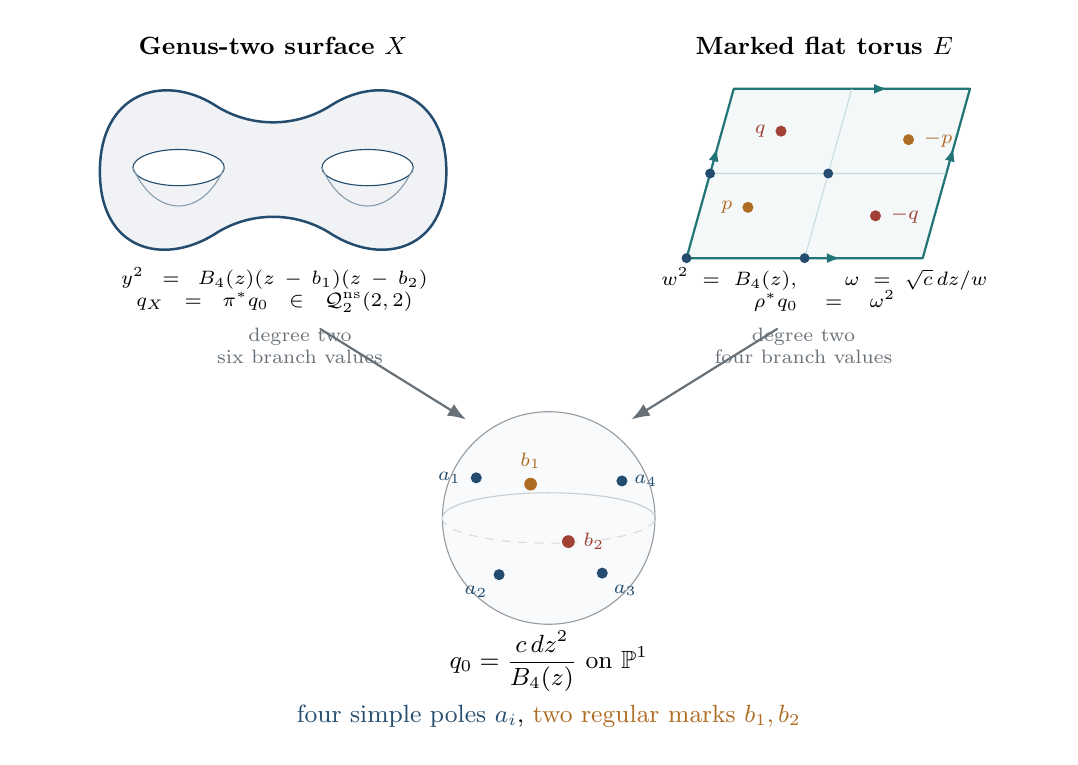
\begin{tikzpicture}[font=\small,>=Latex,line cap=round,line join=round]
  \node[font=\bfseries\small] at (-3.5,3.75) {Genus-two surface $X$};
  \begin{scope}[shift={(-3.5,2.15)}]
    \filldraw[fill=mpblue!7,draw=mpblue,line width=.9pt]
      (-2.2,0) .. controls (-2.2,1) and (-1.4,1.25) .. (-.75,.85)
      .. controls (-.3,.55) and (.3,.55) .. (.75,.85)
      .. controls (1.4,1.25) and (2.2,1) .. (2.2,0)
      .. controls (2.2,-1) and (1.4,-1.2) .. (.75,-.8)
      .. controls (.3,-.5) and (-.3,-.5) .. (-.75,-.8)
      .. controls (-1.4,-1.2) and (-2.2,-1) .. (-2.2,0);
    \filldraw[fill=white,draw=mpblue] (-1.2,.05) ellipse (.58 and .23);
    \filldraw[fill=white,draw=mpblue] (1.2,.05) ellipse (.58 and .23);
    \draw[mpblue!55] (-1.78,.05) .. controls (-1.5,-.6) and (-.9,-.6) .. (-.62,.05);
    \draw[mpblue!55] (.62,.05) .. controls (.9,-.6) and (1.5,-.6) .. (1.78,.05);
  \end{scope}
  \node[align=center,font=\scriptsize,text width=6cm] at (-3.5,.65)
    {$y^2=B_4(z)(z-b_1)(z-b_2)$\\$q_X=\pi^*q_0\in\mathcal Q_2^{\mathrm{ns}}(2,2)$};
  \node[font=\bfseries\small] at (3.5,3.75) {Marked flat torus $E$};
  \begin{scope}[shift={(1.75,1.05)},x={(3cm,0cm)},y={(.6cm,2.15cm)}]
    \filldraw[fill=mpteal!5,draw=mpteal,line width=.8pt] (0,0)--(1,0)--(1,1)--(0,1)--cycle;
    \draw[mpteal!25] (.5,0)--(.5,1) (0,.5)--(1,.5);
    \draw[->,mpteal] (.35,0)--(.65,0);\draw[->,mpteal] (.35,1)--(.65,1);
    \draw[->,mpteal] (0,.35)--(0,.65);\draw[->,mpteal] (1,.35)--(1,.65);
    \foreach \p in {(0,0),(.5,0),(0,.5),(.5,.5)}\fill[mpblue] \p circle (1.8pt);
    \fill[mpochre] (.2,.3) circle (2pt) node[left=2pt,font=\scriptsize] {$p$};
    \fill[mpochre] (.8,.7) circle (2pt) node[right=2pt,font=\scriptsize] {$-p$};
    \fill[mpred] (.25,.75) circle (2pt) node[left=2pt,font=\scriptsize] {$q$};
    \fill[mpred] (.75,.25) circle (2pt) node[right=2pt,font=\scriptsize] {$-q$};
  \end{scope}
  \node[align=center,font=\scriptsize,text width=5.5cm] at (3.5,.65)
    {$w^2=B_4(z),\qquad \omega=\sqrt c\,dz/w$\\$\rho^*q_0=\omega^2$};
  \draw[->,mpgray,line width=.8pt] (-2.9,.15)--(-1.05,-1.0)
    node[midway,above left,font=\scriptsize,align=center] {degree two\\six branch values};
  \draw[->,mpgray,line width=.8pt] (2.9,.15)--(1.05,-1.0)
    node[midway,above right,font=\scriptsize,align=center] {degree two\\four branch values};
  \begin{scope}[shift={(0,-2.25)}]
    \filldraw[fill=mpblue!3,draw=mpgray!70] (0,0) circle (1.35);
    \draw[mpgray!25,dashed] (-1.35,0) arc (180:360:1.35 and .32);
    \draw[mpgray!35] (-1.35,0) arc (180:0:1.35 and .32);
    \fill[mpblue] (-.92,.51) circle (2pt) node[left=2pt,font=\scriptsize] {$a_1$};
    \fill[mpblue] (-.63,-.72) circle (2pt) node[below left=1pt,font=\scriptsize] {$a_2$};
    \fill[mpblue] (.68,-.7) circle (2pt) node[below right=1pt,font=\scriptsize] {$a_3$};
    \fill[mpblue] (.93,.47) circle (2pt) node[right=1pt,font=\scriptsize] {$a_4$};
    \fill[mpochre] (-.23,.43) circle (2.3pt) node[above=2pt,font=\scriptsize] {$b_1$};
    \fill[mpred] (.25,-.3) circle (2.3pt) node[right=2pt,font=\scriptsize] {$b_2$};
  \end{scope}
  \node[align=center] at (0,-4.3)
    {$q_0=\displaystyle\frac{c\,dz^2}{B_4(z)}$ on $\mathbb P^1$\\[4pt]
     \textcolor{mpblue}{four simple poles $a_i$},
     \textcolor{mpochre}{two regular marks $b_1,b_2$}};
\end{tikzpicture}
\caption[The genus-two and marked-torus double covers]{The two double covers used on the nonsquare genus-two stratum
$\mathcal Q_2^{\mathrm{ns}}(2,2)$. The cover $X\to\mathbb P^1$ branches
at all six marked values; the orientation cover $E\to\mathbb P^1$
branches only at the four poles. The two regular marks lift to the pairs
$\{p,-p\}$ and $\{q,-q\}$. Blue points in the torus diagram represent
the four classes in $E[2]$, with boundary identifications understood.
This is a diagram of flat differentials, distinct from the hyperbolic
six-cone-point quotient metric.}
\label{fig:mono-double-covers}
\end{figure}
% END INLINE FIGURE

\subsection{A homogeneous finite cover}
\label{subsec:genus2homogeneous}

Choose a full symplectic level-two structure on the torus and
choose an ordering and one lift from each of the two pairs
$\{\pm p\},\{\pm q\}$.  Together with the origin, level two
labels the four two-torsion points and hence the four poles.  Set
\[
 \Gamma_2=\ker\bigl(SL_2(\ZZ)\to SL_2(\ZZ/2\ZZ)\bigr),
 \qquad
 G_2=SL_2(\RR)\ltimes(\RR^2\oplus\RR^2),
\]
where $SL_2(\RR)$ acts in the standard way on both vector factors.
Our group law and right-quotient convention are
\begin{align}
 (A,u_1,u_2)(B,v_1,v_2)
   &=(AB,u_1+Av_1,u_2+Av_2),\\
 Y_2&=G_2/(\Gamma_2\ltimes(\ZZ^2\oplus\ZZ^2)).
 \label{eq:genus2Y2}
\end{align}
A representative $(A,u_1,u_2)$ describes the area-one torus
$\RR^2/A\ZZ^2$ with marked points $[u_1],[u_2]$.
Right multiplication by $(\gamma,n_1,n_2)$ changes the
representative to
\[
 (A\gamma,u_1+An_1,u_2+An_2),
\]
which is exactly change of the lattice basis preserving level two
and change of the two point lifts.  The presence of $-I$ in
$\Gamma_2$ causes no singularity in this homogeneous quotient:
right translation by a discrete subgroup on a Lie group is free.
Here $A$ and $-A$ give the same physical lattice and the same
level-two data.  A finer congruence level gives an additional finite cover. The spectral
argument below uses level two specifically; its conclusion about the
base spectrum is not automatically inherited by further covers.

Delete the locus where one of the points is two-torsion or where
$[u_1]=\pm[u_2]$, and call the resulting open set $Y_2^\circ$.
In each torus fiber the deleted set is a finite union of real
codimension-two subtori.  It has Haar measure zero and its
complement is connected.  Since the base $SL_2(\RR)/\Gamma_2$ is
connected, so is $Y_2^\circ$.
Forgetting the finite marking choices gives a finite equivariant
local parameterization of $\mathcal Q^{\mathrm{ns},1}_2(2,2)$.
The finite choices include the distinguished origin over a pole,
the level structure, the ordering of the two regular marks, and
their signs.  Their changes preserve Haar measure and commute
with the $SL_2(\RR)$ action; the stratum is their finite quotient.
Over the coarse-moduli locus without additional automorphisms
this is an ordinary finite covering.  If one retains the
ubiquitous genus-two hyperelliptic involution in the orbifold
stabilizers, its fixed order-two contribution must also be
included in unnormalized volume conventions.  No infinite
marking choice is being discarded in this finite-cover statement.

The flow is left multiplication:
\begin{equation}
 g_t[A,u_1,u_2]
   =[a_tA,a_tu_1,a_tu_2],
 \qquad a_t=\diag(e^t,e^{-t}).
 \label{eq:genus2homflow}
\end{equation}
The admissible set $Y_2^\circ$ is invariant under this action.
Although the coordinates $\xi_i=A^{-1}u_i\pmod{\ZZ^2}$ are
unchanged in a fixed lattice chart, a change $A\mapsto A\gamma$
changes them by $\xi_i\mapsto\gamma^{-1}\xi_i$.  Therefore they
are not globally fixed torus coordinates on the quotient.
This monodromy is essential in the later Fourier calculation.

\subsection{Haar measure and the period lattice}
\label{subsec:genus2haarmeasure}

The group $G_2$ is unimodular, and its Haar measure is
\[
 \dd A\,\dd u_1\,\dd u_2,
\]
where $\dd A$ is Haar measure on $SL_2(\RR)$.
In a local lattice chart, $u_i=A\xi_i$ and $\det A=1$, so its
quotient measure is the product of modular Haar measure and
Lebesgue probability on $(\RR^2/\ZZ^2)^2$.
The modular quotient has finite Haar volume and each torus fiber
has volume one, hence $Y_2$ has finite volume.

Before area normalization, local coordinates are the two complex
lattice periods and the two complex positions of the marked
points.  These are four complex coordinates, agreeing with
\[
 \dim_{\CC}\mathcal Q^{\mathrm{ns}}_2(2,2)=4.
\]
The covering construction transports these coordinates to
quadratic-differential period coordinates by a fixed linear map
on each marked chart.  This can be seen without a global
classification theorem.  The orientation cover of $q_X$ is the
fiber product
\[
 \widehat X:\quad
 w^2=B_4(z),\qquad t^2=(z-b_1)(z-b_2),
 \qquad y=wt,
 \qquad \widehat\omega=\sqrt c\,\frac{\dd z}{w}.
\]
Its map to $E$ is a double cover branched at
$\{p,-p,q,-q\}$.  Thus its relative periods are integral linear
combinations of torus periods and marked-point positions, after
paths and lifts have been fixed.  Transfer on absolute cycles and
paths between $p$ and $-p$, or between $q$ and $-q$, recover the
torus periods and twice the point positions, up to periods.
Consequently the inverse change of coordinates is rational
linear.  The integral period lattices are commensurable; factors
of two can occur, so the map need not be unimodular.  This is the
period-coordinate construction underlying the stratum measure
\cite[Sections~1.1.1--1.1.2]{LanneauComponents}.

It follows that the transported Masur--Veech measure is a constant
multiple of Lebesgue measure in these cone coordinates.  More
explicitly, write the torus area as $s>0$, put $A=\sqrt{s}\,B$
with $\det B=1$, and use the point coordinates $\xi_i=A^{-1}u_i$.
Up to a fixed positive constant the cone measure is
\[
 s^3\,\dd s\,\dd B\,\dd\xi_1\,\dd\xi_2.
\]
Restricting by area as in~\eqref{eq:genus2equalareas} therefore
makes the unit-area measure a constant multiple of Haar measure
on $Y_2$.  After
normalizing to probability and accounting for the finite covering,
the measures agree.  No numerical identity between unnormalized
volumes is asserted without a choice of lattice and labeling
conventions.  The measure-zero exclusions in $Y_2\setminus
Y_2^\circ$ do not affect this probability identification.

For observables compactly supported inside $Y_2^\circ$, extension
by zero gives smooth observables on the homogeneous space.  Thus
estimates proved there pass to the stratum after lifting the
observables and, if necessary, averaging over the finite markings.
For observables which grow near collisions, extension and norm
control require additional estimates; a null collision set alone
is not a bound on such observables.


\subsection{Fourier decomposition and temperedness}
\label{subsec:markedtorusconverse}

The affine homogeneous model admits a direct calculation which does
not use a general Teichm\"uller mixing theorem. Let
\[
 G=\operatorname{SL}_2(\RR),\qquad
 \mathsf A=G\ltimes\operatorname{Mat}_{2\times2}(\RR),\qquad
 \Lambda=\Gamma\ltimes\operatorname{Mat}_{2\times2}(\ZZ),
\]
where $\Gamma=\Gamma(2)$ initially. The group law is
\[
 (g,v)(g',v')=(gg',v+gv').
\]
Set $Y_2=\mathsf A/\Lambda$, with Haar probability measure $\mu$, and
let $a_t=\diag(e^t,e^{-t})$ act by left translation. A point is a
unit-area lattice together with two marked vectors modulo that
lattice. If one counts the origin as a marked point, this is a
torus with three ordered marked points. Coincidence loci have
measure zero and may be removed. Any application to a particular
quadratic stratum uses its separately established geometric
identification with this model or a finite quotient; an arbitrary
finite cover cannot be discarded without checking its base spectrum.

\subsubsection*{Fiber Fourier coefficients and their stabilizers}

Write $v=gu$, with $u\in\operatorname{Mat}_{2\times2}(\RR)/
\operatorname{Mat}_{2\times2}(\ZZ)$. Then
\[
 (g,u)\sim(g\gamma,\gamma^{-1}u),\qquad
 a_t(g,u)=(a_tg,u).
\]
For $F\in L^2(Y_2)$ expand, in the $L^2$ sense,
\begin{equation}
 F(g,u)=\sum_{M\in\operatorname{Mat}_{2\times2}(\ZZ)}
   F_M(g)e^{2\pi i\tr(M^Tu)}.
 \label{eq:markedtorusfourier}
\end{equation}
The equivariance relation is
\begin{equation}
 F_M(g\gamma)=F_{\gamma^{-T}M}(g).
 \label{eq:markedtorusequivariance}
\end{equation}
Consequently each $\Gamma$-orbit of frequency matrices contributes
a $G$-invariant summand isometric to
\begin{equation}
 L^2(G/\Gamma_M),\qquad
 \Gamma_M=\{\gamma\in\Gamma:\gamma^TM=M\}.
 \label{eq:markedtorusinduction}
\end{equation}
Indeed, Parseval followed by unfolding the orbit sum gives
\[
 \int_{G/\Gamma}
       \sum_{M'\in\Gamma\cdot M}|F_{M'}(g)|^2\,\dd g
   =\int_{G/\Gamma_M}|F_M(g)|^2\,\dd g.
\]

The stabilizers are elementary. If $M=0$, the summand is
$L^2(G/\Gamma)$. If $M$ has rank two, $\Gamma_M=\{1\}$.
If $M$ has rank one, write $M=vw^T$, with $v$ a primitive
integral column vector and $w\ne0$ an integral column vector.
Then $\Gamma_M$ fixes $v$ under the transpose action. It is a
subgroup conjugate to a discrete unipotent group, hence is
amenable. For example, if $v=(1,0)^T$ and $\Gamma=\Gamma(2)$,
\[
 \Gamma_M=
 \left\{\begin{pmatrix}1&0\\2n&1\end{pmatrix}:n\in\ZZ\right\}.
\]
No transitivity assertion about primitive vectors under $\Gamma(2)$
is required: one simply sums over all its frequency orbits. The same
rank distinction appears in the fiber Fourier analysis of
\cite[Section~4, especially Lemma~4.3]{StrombergssonVishe}.

The trivial representation of an amenable group is weakly
contained in its regular representation. Induction preserves
weak containment and takes the regular representation of a closed
subgroup to that of $G$. Thus every nonzero-frequency summand
in~\eqref{eq:markedtorusinduction} is tempered. See
\cite[Lemma 2.3 and Remark 2.4]{BenoistKobayashi}.
The whole orthogonal complement of the fiber average is tempered,
including its countably many frequency orbits. This gives uniform
control of their sum; there is no frequency-dependent implied
constant left to sum. Explicitly, for every $f\in C_c(G)$, all
summands satisfy $\|\pi_{[M]}(f)\|\leq\|\lambda_G(f)\|$;
their Hilbert direct sum satisfies the same inequality.

This simple stabilizer argument is enough for the present rate
estimate. It does not claim a complete irreducible spectral
decomposition. The corresponding finer decomposition for one
relative marked vector is developed in
\cite{AthreyaLagaceMollerRaum}; in particular, that paper's genuine
part contains no complementary series.

\subsubsection*{The base spectrum at level two}

The quotient $\Gamma(2)\backslash\HH$ is the thrice-punctured
sphere. The finite-area theorem of
\cite[Theorem 2]{OtalRosas} states that the discrete eigenvalue
$\lambda_{2g-2+n}$ exceeds $1/4$, counting $\lambda_0=0$ and
including residual as well as cuspidal eigenvalues. For $(g,n)=(0,3)$,
there is therefore no positive discrete eigenvalue at or below
$1/4$. The continuous spectrum starts at $1/4$.
Since $-I\in\Gamma(2)$, the base representation factors through
$\operatorname{PSL}_2(\RR)$. All non-tempered nontrivial representations of
$\operatorname{PSL}_2(\RR)$ in this setting are spherical
complementary-series representations and would produce a
Laplacian eigenvalue in $(0,1/4)$; this is the $d=1$ specialization of
the unitary-dual description in~\cite[Section~1]{EdwardsOhMixing}.
It follows that
$L^2_0(G/\Gamma(2))$ is tempered. The same conclusion holds for
$\Gamma=\operatorname{SL}_2(\ZZ)$, by pullback from that quotient
to the level-two cover.

Combining the base and nonzero-frequency parts proves that
\begin{equation}
 L^2_0(Y_2)\quad\hbox{is a tempered $G$-representation}
 \label{eq:markedtorusalltempered}
\end{equation}
for either of these two choices of $\Gamma$. The statement does
not automatically hold for a further finite-index subgroup.

\subsection{A global correlation bound with an explicit constant}

Let $K=\operatorname{SO}(2)$, with angular generator $\Theta$,
normalized so that the $n$th character has derivative $in$.
Use the norm
\begin{equation}
 \mathcal S_1(F)^2=\|F\|_2^2+\|\Theta F\|_2^2.
 \label{eq:markedtorusKnorm}
\end{equation}
The angle is the ordinary matrix rotation angle: on the orientation
cover, $\omega$ changes to $e^{i\theta}\omega$, so the genus-two
quadratic differential changes to $e^{2i\theta}q_X$. Thus this
normalization is twice differentiation in the phase of $q_X$.
Write $F^\circ=F-\mu(F)$ and $G^\circ=G-\mu(G)$.
The Cowling--Haagerup--Howe bound for a tempered representation is
\[
 |\langle\pi(g)v,w\rangle|
 \leq\Xi(g)\|v\|\|w\|
       \sqrt{\dim Kv\,\dim Kw}
\]
for $K$-finite vectors; see
\cite[Proposition 2.6]{BenoistKobayashi} and
\cite{CowlingHaagerupHowe}. For single $K$-types the two
dimension factors equal one. Decomposing into $K$-types and
using Cauchy--Schwarz gives
\[
 \sum_{n\in\ZZ}\|F_n\|_2
 \leq\left(\sum_{n\in\ZZ}(1+n^2)^{-1}\right)^{1/2}
       \mathcal S_1(F)
 =\sqrt{\pi\coth\pi}\,\mathcal S_1(F).
\]
Here the subscript denotes $K$-type, distinct from the matrix
frequency in~\eqref{eq:markedtorusfourier}.

For $e_1=(1,0)^T$, the spherical principal-series realization gives
$\Xi(a_t)=\int_K|a_tke_1|^{-1}\,\dd k$, with Haar probability on $K$.
Using $u=\tan\theta$ on a quadrant gives, in our time normalization,
the elementary integral
\begin{equation}
 \Xi(a_t)=\frac2\pi e^{-t}
   \int_0^\infty
    \frac{\dd u}{\sqrt{(1+u^2)(1+e^{-4t}u^2)}}
 \leq\frac4\pi(1+t)e^{-t},\qquad t\geq0.
 \label{eq:markedtorusXi}
\end{equation}
For the inequality, split the integral at $u=1$ and $u=e^{2t}$.
The three contributions are at most $1$, $2t$, and $1$.
\begin{theorem}[An explicit marked-torus correlation bound]
\label{thm:markedtorusmixing}
For Haar probability measure on $Y_2$ and all $F,G$ in the domain
of the rotation generator, the following inequality holds for $t\geq0$:
\begin{equation}
 \begin{split}
 \left|\int_{Y_2}\overline F\,(G\circ a_t)\,\dd\mu
       -\overline{\mu(F)}\mu(G)\right|
 \leq4\coth\pi\,(1+t)e^{-t}
       \mathcal S_1(F^\circ)\mathcal S_1(G^\circ).
 \end{split}
 \label{eq:markedtorusexplicitmix}
\end{equation}
The same estimate holds on $\mathcal Q^{\mathrm{ns},1}_2(2,2)$
with its probability-normalized Masur--Veech measure and the induced
rotation norm.
\end{theorem}
\begin{proof}
The preceding $K$-type estimate and~\eqref{eq:markedtorusXi} apply
to the tempered representation~\eqref{eq:markedtorusalltempered}.
Remove the constant components to obtain the displayed covariance.
The geometric statement follows by pulling observables back to the
finite model of Section~\ref{subsec:genus2homogeneous}; probability
normalization preserves the norms and the correlation.
\end{proof}
Centering the functions does not increase $\mathcal S_1$.
The norm needs only one rotation derivative; neither derivatives in
the marked-point coordinates nor compact support are required.
This is global on the finite-volume affine quotient. No compact
cutoff or unquantified cusp-tail estimate enters this inequality.
The polynomial factor allows every pure exponential rate
$e^{-(1-\varepsilon)t}$, but not a uniform constant times $e^{-t}$
from this argument. More explicitly, for $0<\varepsilon\leq1$ one
may replace $4\coth\pi(1+t)e^{-t}$ by
$4\coth\pi\,\varepsilon^{-1}e^{-(1-\varepsilon)t}$.
For the convention $a_t=\diag(e^{t/2},e^{-t/2})$, replace $t$
by $t/2$ throughout.

\subsection{An exact finite lattice sum with two endpoint weights}

The following unfolding supplies a concrete counting statistic.
For $\varphi,\psi\in C_c^\infty(\mathsf A)$ let
\[
 P\varphi(h\Lambda)=\sum_{\lambda\in\Lambda}\varphi(h\lambda),
 \qquad F=P\varphi,\quad G=P\psi.
\]
Normalize Haar measure $\dd h$ so that $\mathsf A/\Lambda$ has volume one.
For fixed $t$ define the overlap weight
\begin{equation}
 W_t^{\varphi,\psi}(\lambda)
 =\int_{\mathsf A}\overline{\varphi(h)}\,
                   \psi(a_th\lambda)\,\dd h.
 \label{eq:markedtorusweight}
\end{equation}
Only finitely many $\lambda$ contribute, since any such lattice
element lies in the compact set
$(\operatorname{supp}\varphi)^{-1}a_{-t}
\operatorname{supp}\psi$. In coordinates
$h=(g,v)$ and $\lambda=(\gamma,m)$, the weight is explicitly
\begin{equation}
 W_t^{\varphi,\psi}(\gamma,m)
 =\int_G\int_{\operatorname{Mat}_{2\times2}(\RR)}
    \overline{\varphi(g,v)}\,
    \psi\bigl(a_tg\gamma,a_t(v+gm)\bigr)\,\dd v\,\dd g.
 \label{eq:markedtorusweightcoordinates}
\end{equation}
Unfolding the periodization of the first observable gives exactly
\begin{equation}
 \sum_{\lambda\in\Lambda}W_t^{\varphi,\psi}(\lambda)
   =\int_{Y_2}\overline F\,(G\circ a_t)\,\dd\mu.
 \label{eq:markedtorusexactcount}
\end{equation}
The weights are nonnegative when $\varphi$ and $\psi$ are
nonnegative. For arbitrary observables they are signed or complex.
Thus~\eqref{eq:markedtorusexactcount} is a finite weighted return
sum, not an assertion about an unweighted sharp orbit count.

The unstable Jacobian exponent is $4$: conjugation by $a_t$
expands the upper-unipotent direction in $\mathfrak{sl}_2$ by
$e^{2t}$ and the two expanding translation directions by $e^t$
each. Accordingly define the normalized return statistic and its
cumulative version, for $T\geq1$, by
\[
 \mathcal N_{\varphi,\psi}(t)
   =e^{4t}\sum_{\lambda\in\Lambda}
                     W_t^{\varphi,\psi}(\lambda),\qquad
 \mathcal A_{\varphi,\psi}(T)
   =\int_1^T\mathcal N_{\varphi,\psi}(t)\,\dd t.
\]
This normalization uses the affine model's unstable Jacobian. It
does not use the polar Jacobian of full Teichm\"uller space.
Since $\mu(P\varphi)=\int_{\mathsf A}\varphi\,\dd h$,
\eqref{eq:markedtorusexplicitmix} gives the explicit remainder
\begin{equation}
 \begin{split}
 \left|\mathcal A_{\varphi,\psi}(T)
    -\overline{\mu(F)}\mu(G)\frac{e^{4T}-e^4}{4}\right|
 \leq\frac43\coth\pi\,(1+T)e^{3T}
       \mathcal S_1(F^\circ)\mathcal S_1(G^\circ).
 \end{split}
 \label{eq:markedtoruscountremainder}
\end{equation}
Equivalently, with $R=e^T$, this is an $O(R^3\log R)$
remainder against an $R^4$ main term, with a displayed norm bound.
Here $R=e^T$ is an exponential-time parameter; identifying it with
hyperbolic curve length, intersection number, or square-tiled area
would require a separate comparison. The estimate follows simply from
$\int_1^T(1+t)e^{3t}\dd t\leq\tfrac13(1+T)e^{3T}$.

These norms can also be bounded using the original compactly
supported weights. If $K_0\subset \mathsf A$ contains their supports and
\[
 M_{K_0}=\#(\Lambda\cap K_0^{-1}K_0),
\]
then Cauchy--Schwarz in the locally finite periodization gives
\[
 \mathcal S_1(P\varphi)
  \leq\sqrt{M_{K_0}}
       \bigl(\|\varphi\|_{L^2(\mathsf A)}^2+
              \|\Theta\varphi\|_{L^2(\mathsf A)}^2\bigr)^{1/2},
\]
and similarly for $\psi$. All quantities in this bound are finite
for the chosen compact supports.

Define the flow generator by
$V\psi(h)=\left.\frac{\dd}{\dd s}\right|_{s=0}\psi(a_sh)$.
Periodization commutes with this generator:
$V(P\psi)=P(V\psi)$. Therefore inserting the terminal weight
$(4+V)\psi$ gives the exact identity
\begin{equation}
 \begin{split}
 \mathcal A_{\varphi,(4+V)\psi}(T)
  &=e^{4T}\int_{Y_2}\overline F\,(G\circ a_T)\,\dd\mu\\
  &\quad-e^4\int_{Y_2}\overline F\,(G\circ a_1)\,\dd\mu.
 \end{split}
 \label{eq:markedtorusderivativeweight}
\end{equation}
There is no convolution operator to commute past $V$, and no
unjustified differentiation of a counting asymptotic.
The quantitative norm required for this terminal test is
$\mathcal S_1((4+V)G)\leq4\mathcal S_1(G)+\mathcal S_1(VG)$.
It includes $\|\Theta VG\|_2$; the generators $\Theta$ and $V$
do not commute, and this mixed derivative is not omitted.


\subsection{What the marked-torus calculation settles}
\label{subsec:genus2torusscope}

The compact polyhedron encodes the genus-two hyperbolic base, whereas the
marked flat torus encodes the nonsquare $(2,2)$ differential and its flow.
They use different intrinsic metrics and are linked by the same six branch
values. The affine model gives an exact Fourier decomposition, an explicit
global correlation bound, and the finite weighted return sum with
remainder~\eqref{eq:markedtoruscountremainder}. These are conclusions of the
calculation, not hypotheses imported from general Teichm\"uller mixing.
The inputs are classical: amenability and induction, the
Cowling--Haagerup--Howe bound, the elementary $SL_2$ spherical function,
and the absence of positive small spectrum on the thrice-punctured sphere.
Related marked-torus harmonic analysis is already developed in
\cite{StrombergssonVishe,AthreyaLagaceMollerRaum}; no novelty claim for that
machinery is intended.

The derivative identity~\eqref{eq:markedtorusderivativeweight} also makes
the counting converse exact in this model. After subtracting the product
of means, a bound for the terminal test $(4+V)G$ recovers the correlation
at $T$ with the same exponential saving. In the proof here the direction
is Fourier/representation theory to correlations and hence to counts.
The identity identifies the reverse implication as well, without making
the proof circular.

The restriction to the chosen stratum remains substantial. Although it
meets every genus-two conformal base, its unit-area dimension is seven;
the principal unit stratum has dimension eleven. The affine expanding
Jacobian is $e^{4t}$, whereas the full genus-two Teichm\"uller polar kernel
in Section~\ref{sec:pairconverse} has exponent $6$. The two kernels cannot
be substituted for one another. Section~\ref{sec:coefficientobservables}
constructs selected primitive-arc observables from the coefficient data
with controlled geometric norms. A comparison with the full orbit kernel,
and uniform stability of the nonlinear coefficient extraction, remain
open. In particular, the $O(R^3\log R)$ estimate above is not an error
term for the unweighted count of connected simple closed geodesics.
A comparison with that count, or an extension to the principal stratum
$\mathcal Q^1_2(1^4)$, is a further problem.




\section{From simple-curve coefficients to controlled observables}
\label{sec:coefficientobservables}

The preceding section supplies an explicit analytic norm for its mixing
estimate. We now connect that norm to a selected family of simple curves
and their coefficient distributions. The genus-one norm-ball obstruction
first fixes the attainable scale of sharp remainders. Primitive
pole-to-pole arcs then give geometric coefficient observables with
uniform rotation and terminal-derivative bounds. Exact affine Gaussian
calculations provide independent tests of the analytic estimates.
Throughout, a fixed-surface sharp count, a moduli-averaged covariance,
and the conditioning of coefficient extraction remain separate problems.

\subsection{The norm-ball obstruction and the correct error scale}
\label{subsec:normballbarrier}

The genus-one length norm gives a necessary benchmark for any passage from
smooth return estimates to sharp simple-curve counting. Let $X$ be a fixed
complete hyperbolic once-punctured torus, and let $B_X$ be the unit ball of
the McShane--Rivin length norm on $H_1(X;\RR)\simeq\RR^2$. Put
\[
 A_X(L)=\#(LB_X\cap\ZZ^2),\qquad
 P_X(L)=\#(LB_X\cap\ZZ^2_{\mathrm{prim}}).
\]
The first count includes the origin and nonprimitive classes. The second
counts oriented primitive classes; the count of unoriented simple closed
geodesics is $N_X(L)=\tfrac12P_X(L)$. Elementary planar lattice counting
and M\"obius inversion give
\begin{align}
 A_X(L)&=\operatorname{Area}(B_X)L^2+O_X(L),\label{eq:normballall}\\
 P_X(L)&=\frac{\operatorname{Area}(B_X)}{\zeta(2)}L^2
           +O_X(L\log L).\label{eq:normballprimitive}
\end{align}
Indeed, $P_X(L)=\sum_d\mu(d)(A_X(L/d)-1)$, with $d\ll_X L$;
the boundary errors sum as $L\sum_{d\ll_X L}d^{-1}$. These are the
upper estimates behind \cite[Theorem~4.1]{McShaneRivinTori}, with the
orientation factor made explicit here.

The next theorem in that paper concerns a dense set of hyperbolic
structures. Its mechanism is an infinitely flat boundary point whose
supporting normal is rational with respect to the homology lattice.
The subsequent Conjecture~4.3 proposes an $O(L^{1/2+\varepsilon})$ error
for the modular torus; thus the obstruction is not asserted there for
every individual surface. The phrase ``at least $O(L)$'' in Theorem~4.2
should be separated from the literal modern assertion
$\limsup|E_X(L)|/L>0$. The elementary argument below proves the precise
consequence needed here: no fixed improvement of the exponent below one
is possible under the stated flat-point hypothesis. We do not use it to
claim a literal $\Omega(L)$ bound.

\begin{proposition}[A primitive-row obstruction]
\label{prop:normballflatrow}
Let $B\subset\RR^2$ be a strictly convex compact body with the origin
in its interior. Suppose that $p\in\partial B$ has irrational radial
direction, a rational supporting normal, and infinite graph-flatness.
Then, for
\[
 E_B(L)=\#(LB\cap\ZZ^2_{\mathrm{prim}})
       -\frac{\operatorname{Area}(B)}{\zeta(2)}L^2,
\]
and every $\varepsilon>0$, there are $c_\varepsilon>0$ and arbitrarily
large $L$ such that
\begin{equation}
 |E_B(L)|\geq c_\varepsilon L^{1-\varepsilon}.
 \label{eq:normballlowerpower}
\end{equation}
In particular $E_B(L)=O(L^{1-\eta})$ fails for every fixed $\eta>0$.
\end{proposition}

\begin{proof}
An integral unimodular change of coordinates makes the supporting normal
vertical. Write $p=(\alpha,h)$, with $h>0$ and $\alpha/h$ irrational.
Near $p$, the upper boundary has the form
\[
 y=h-f(x-\alpha),\qquad f(0)=0,
\]
where $f\geq0$ is convex. Infinite graph-flatness means that for every
integer $N>2$ there are $C_N,\rho_N>0$ such that
\[
 0\leq f(s)\leq C_N|s|^N\qquad (|s|\leq\rho_N).
\]
Fix $N$, let $n$ run through primes, and set
\[
 L_n=\frac nh,\qquad \delta_n=L_n^{-1},\qquad L_n^+=L_n+\delta_n.
\]
The line $y=n$ supports $L_nB$ at the single point
$(L_n\alpha,n)$. Its first coordinate is irrational, so this row
contains no lattice point of $L_nB$.

In $L_n^+B$, the same row lies a normalized depth
$h\delta_n/L_n^+$ below the supporting line. Therefore it contains the
horizontal interval centered at $L_n^+\alpha$ with half-width
\[
 r_n=\min\left\{
 \left(\frac h{2C_N}\right)^{1/N}
 (L_n^+)^{1-1/N}\delta_n^{1/N},\ \frac n4
 \right\}.
\]
For sufficiently large $n$ the local graph description applies, the
first quantity realizes the minimum, and
\[
 r_n\asymp_{B,N}L_n^{1-2/N}.
\]
The interval has length at most $n/2$. Among its integer points
$(k,n)$, at most one has $n\mid k$; every other point is primitive
because $n$ is prime. Thus
\[
 P_B(L_n^+)-P_B(L_n)\geq 2r_n-O(1).
\]
The change in the quadratic main term is bounded, since
\[
 (L_n^+)^2-L_n^2=2+L_n^{-2}.
\]
It follows that
\[
 \max\{|E_B(L_n)|,|E_B(L_n^+)|\}
 \geq c_{B,N}L_n^{1-2/N}
\]
for all sufficiently large primes $n$. Choose $N>2/\varepsilon$ to
obtain the assertion. To rule out a proposed $O(L^{1-\eta})$ estimate,
apply the assertion with $0<\varepsilon<\eta$.
\end{proof}

The proof works directly with primitive classes, so no cancellation in a
M\"obius sum needs to be controlled. The short interval
$[L_n,L_n+L_n^{-1}]$ acquires many new primitive points along a nearly
flat supporting row, while its predicted main-term increment stays
bounded. Infinite flatness alone does not force the row length to be a
positive fraction of $L_n$; that is why the proof gives an exponent-one
barrier, not a literal linear lower bound. The distinction between a
fixed-surface estimate, an estimate uniform over moduli, and a smoothed
estimate must be retained.

\subsection{The Fourier and spectral meaning of the obstruction}
\label{subsec:normballspectral}

The flatness obstruction has a direct oscillatory-integral interpretation.
For illustration, suppose a localized smooth boundary arc has graph
\[
 y=h-f(x),\qquad f(x)=a x^k+O(x^{k+1}),\quad a>0,
\]
where $k\geq2$ is even. Apply smooth cutoffs supported near this arc
and equal to one at the supporting point. Integrating the localized
indicator in the normal coordinate first gives, up to rapidly decreasing
terms,
\[
 -\frac{e^{-2\pi i r h}}{2\pi i r}
       \int \chi(x)e^{2\pi i r f(x)}\,\dd x.
\]
The substitution $x=r^{-1/k}u$ in the stationary-phase calculation gives
\begin{equation}
 \widehat{\chi_0\mathbf1_B}(r\nu)
   =c_{a,k}\,e^{-2\pi i r h}r^{-1-1/k}
     +o(r^{-1-1/k}),\qquad c_{a,k}\ne0.
 \label{eq:normballfinitephase}
\end{equation}
where $\nu$ is the chosen normal direction and $\chi_0$ is the localized
cutoff. The familiar nondegenerate exponent is $r^{-3/2}$ when $k=2$;
larger contact order weakens it toward $r^{-1}$. Localization matters:
the contributions of different supporting points can interfere in the
Fourier transform of the whole ball. No global lower bound follows from
discarding those phases.

Under dilation,
\[
 \widehat{\mathbf1_{LB}}(m)=L^2\widehat{\mathbf1_B}(Lm).
\]
Thus a finite-type flat point with a lattice-rational normal contributes
on the scale $L^{1-1/k}$ to the corresponding localized Poisson terms.
For an infinitely flat point there is no fixed finite type to insert in
this formula. Proposition~\ref{prop:normballflatrow} supplies a direct
counting argument in that case, without assuming smooth boundary
regularity at all nearby points or invoking a formal stationary-phase
expansion there.

There is also an exact elementary spectral model. On an auxiliary flat
torus $\RR^2/\ZZ^2$, define the positive self-adjoint Fourier multiplier
\[
 \mathsf P_X e^{2\pi i\langle m,x\rangle}
   =\|m\|_X e^{2\pi i\langle m,x\rangle}.
\]
Norm equivalence gives a discrete spectrum tending to infinity. Its
counting function is $A_X(L)$, and restriction to the closed span of
primitive Fourier modes has counting function $P_X(L)$. Restricting
further to the even part identifies $m$ and $-m$ and gives $N_X(L)$.
This multiplier is defined spectrally; the nonsmooth length norm is not
being asserted to be a classical smooth pseudodifferential symbol.
At a differentiable point $p$ of its unit ball, a supporting covector
$\nu$ satisfies
\[
 \nabla\|\cdot\|_X(p)=\frac{\nu}{\langle\nu,p\rangle}.
\]
Thus a lattice-rational normal is exactly a rational direction for the
translation velocity of the associated Hamiltonian. This explains the
periodic-phase interpretation, without assuming that a global smooth
trace formula applies to the length norm.

The norm-ball discrepancy is therefore a spectral-projector remainder
for this particular length multiplier. Its flat normal directions
produce degenerate phases in a regularized Poisson or trace calculation.
This is distinct from complementary-series spectrum for the
$SL_2(\RR)$ action on the marked-torus moduli space. In particular, it
does not contradict the temperedness statement or the smooth
correlation estimate in Section~\ref{sec:genus2markedtorus}. The
rotation-Sobolev issue depends on what is held fixed. A sharp indicator
of a nonradial region in fixed physical vector coordinates generally
has rotational jumps, so smoothing it introduces growing derivative
norms. By contrast, hyperbolic length is unchanged when the flat charts
are rotated while the underlying conformal surface stays fixed. A sharp
cutoff in that invariant length can therefore lie in the rotation
generator's domain, and a radial flat cutoff can be rotation invariant
as well. Sharpness alone is not an obstruction to the stated mixing
bound. For those invariant observables, the remaining boundary and
regularity issues enter when taking flow derivatives or passing from
an averaged correlation to a fixed-surface counting remainder.

\subsection{A coefficient observable from primitive pole-to-pole arcs}
\label{subsec:primitivepolebridge}

The marked-torus construction supplies an explicit family of simple curves
for which the coefficient data become observables with controlled norms.
This family carries a flat-length cutoff as well as a hyperbolic-length
weight. The two length parameters remain distinct.

Work on the finite labeled model $Y_2$ of
Section~\ref{subsec:genus2homogeneous}. Write
$E=\RR^2/g\ZZ^2$, with its origin one of the four ramification points
of the pillowcase map. Fix a nonzero parity vector
$\delta\in(\ZZ/2\ZZ)^2$. For a nonzero primitive integer vector
$m\equiv\delta\pmod2$, project the straight segment
\[
 [0,gm/2]\subset\RR^2
\]
first to $E$ and then to $E/\{\pm1\}$. It joins the pole at the
origin to the pole corresponding to $\delta/2$.

\begin{lemma}[Primitive directions give simple curves]
\label{lem:primitivepolearcs}
Outside a Haar-null invariant subset of $Y_2$, the preceding segment
projects to an embedded arc avoiding the two regular marked points.
Its lift to the genus-two double cover is a nonseparating simple
closed regular flat geodesic $\alpha_m$, with
\begin{equation}
 \ell_{q_X}(\alpha_m)=|gm|.
 \label{eq:polearcflatlength}
\end{equation}
Opposite vectors give the same curve; distinct primitive directions
modulo sign give distinct free homotopy classes.
\end{lemma}

\begin{proof}
If two parameters $0<s,t<1$ on the segment identify on the pillowcase,
then $(s-t)m\in2\ZZ^2$ or $(s+t)m\in2\ZZ^2$. Primitivity forces
the corresponding scalar to be an even integer. The first case gives
$s=t$, and the second is impossible. Likewise the interior contains no
two-torsion point. The segment hits one of the additional regular marks
only if one of its lifts $p,q$ lies on the closed rational circle
$\RR gm/g\ZZ^2$. For each $m$ this is a null condition in the point
fiber. The union over the countable set of primitive $m$ is still null
and is invariant under the entire $SL_2(\RR)$ action.

The preimage of an embedded arc joining two branch values of a double
cover is a circle. Removing it leaves a connected cover, since the four
other branch values still have nontrivial monodromy; thus the circle is
nonseparating. At its endpoints the sphere flat angle $\pi$ doubles to
$2\pi$, so the two lifted segments join to a regular flat geodesic.
Its length is twice $|gm|/2$. Different directions give intersecting
regular geodesics with distinct tangents at the Weierstrass point over
the origin. Freely homotopic regular geodesics in a nonpositively curved
flat metric lie in a flat cylinder and cannot intersect transversely.
This proves the last assertion.
\end{proof}

Write $\ell_m(q_X)=\ell_X(\alpha_m)$ for the hyperbolic length of the
same topological curve. Proposition~\ref{prop:coefffirstatom} identifies
it as the position of the first atom of $\sigma^X_{\alpha_m}$. In
particular, if a local cutoff $\chi_m$ is one near that atom and
vanishes on the remaining support, then for a
bounded length weight $H$,
\begin{equation}
 H(\ell_m)=
 \frac{\langle\sigma^X_{\alpha_m},H(s)\chi_m(s)\rangle}
      {\langle\sigma^X_{\alpha_m},\chi_m(s)\rangle}.
 \label{eq:polearccoefficientweight}
\end{equation}
For arbitrary bounded Borel $H$, the same statement is interpreted
using the already recovered first-atom location. No assertion that
first-atom extraction is a bounded linear functional is being made.

Choose an even $f\in C_c^2(\RR^2)$ supported in the unit disk, a bounded
Borel function $h:(0,\infty)\to\CC$, and parameters $R\geq1$, $L>0$.
Define
\begin{equation}
 \mathcal F_{\delta;f,h}^{R,L}(q_X)
  =\frac1{2R^2}
    \sum_{\substack{m\in\ZZ^2\ \mathrm{primitive}\\m\equiv\delta\ (2)}}
       f(gm/R)\,h\bigl(\ell_m(q_X)/L\bigr).
 \label{eq:polearcobservable}
\end{equation}
The factor $1/2$ identifies opposite directions. The function is
well defined on $Y_2$: changes of lattice basis preserve the parity
class and relabel the sum. More precisely, define the geometric formula
on the invariant conull admissible set of
Lemma~\ref{lem:primitivepolearcs} and set it to zero on its complement;
this fixes a measurable representative of the same $L^2$ class.
Averaging over the finite labeling choices
gives observables on the unlabelled stratum, with the same norm bounds.
Such an average is an average of selected families; it need not count
their union without multiplicities.

\subsection{Uniform rotation norms, including a sharp hyperbolic cutoff}
\label{subsec:polearcnorms}

Put
\[
 J=\begin{pmatrix}0&-1\\1&0\end{pmatrix},\qquad
 A=\begin{pmatrix}1&0\\0&-1\end{pmatrix},\qquad
 D_Bf(x)=(Bx)\cdot\nabla f(x).
\]
The notation $D_B$ here is a linear vector field on $\RR^2$.

\begin{lemma}[Uniform primitive-vector bound]
\label{lem:polearcprimitivebound}
For every unimodular lattice $g\ZZ^2$ and every $R>0$,
\begin{equation}
 \#\{m\in\ZZ^2:\ m\ \mathrm{primitive},\ |gm|\leq R\}
 \leq 2+2\pi R^2.
 \label{eq:polearcprimitivebound}
\end{equation}
\end{lemma}

\begin{proof}
Two nonparallel lattice vectors $u,v$ have $|\det(u,v)|\geq1$.
If both have length at most $R$, their unoriented angular separation
therefore has sine at least $R^{-2}$. For $R<1$ there is at most one
primitive direction. For $R\geq1$, placing the directions on the circle
of length $\pi$ shows that their number is at most
$\pi/\arcsin(R^{-2})\leq\pi R^2$. Each direction contributes only
the two opposite primitive vectors. The displayed bound covers both
cases without rounding conventions.
\end{proof}

Rotation of the flat charts fixes the underlying conformal surface and
the intrinsic pole-to-pole arcs. Consequently
\[
 \Theta\ell_m=0,
\]
and differentiation of~\eqref{eq:polearcobservable} under rotation
only replaces $f$ by $D_Jf$. Set
\[
 C_*=1+\pi,\qquad
 N_{f,h}=C_*\|h\|_\infty
             \bigl(\|f\|_\infty^2+\|D_Jf\|_\infty^2\bigr)^{1/2}.
\]
The primitive-vector bound proves, uniformly in $R\geq1$ and $L>0$,
\begin{equation}
 \mathcal S_1(\mathcal F_{\delta;f,h}^{R,L})\leq N_{f,h}.
 \label{eq:polearcuniformS1}
\end{equation}
This is global, including the modular cusp. Although the curve labels
can jump as a regular mark crosses a selected arc, the exceptional walls
are $SL_2$-invariant. Along almost every group orbit the labels are fixed
under the natural marking, and the preceding derivatives are legitimate.
Uniform bounds on the difference quotients give the corresponding strong
$L^2$ generator statements.

In particular, Theorem~\ref{thm:markedtorusmixing} now applies to two
observables of the form~\eqref{eq:polearcobservable}, with
\begin{equation}
 |\operatorname{Corr}_t(\mathcal F,\mathcal G)|
 \leq4\coth\pi\,(1+t)e^{-t}\,N_{f,h}N_{\widetilde f,\widetilde h},
 \label{eq:polearccorrelation}
\end{equation}
uniformly in their two flat cutoffs and two hyperbolic-length scales.
The hyperbolic weight may be the sharp cutoff
$h(s)=\mathbf1_{s\leq1}$: its discontinuity costs no rotation derivative.
If the flat weight is radial as well, the whole observable is
$K$-invariant. In that case a sharp disk cutoff is also allowed directly,
and the single-$K$-type matrix-coefficient bound gives the sharper estimate
\begin{equation}
 |\operatorname{Corr}_t(F,G)|
 \leq\Xi(a_t)\|F^\circ\|_2\|G^\circ\|_2
 \leq\frac4\pi(1+t)e^{-t}\|F^\circ\|_2\|G^\circ\|_2.
 \label{eq:polearcKfixedcorrelation}
\end{equation}
No rotational smoothing is needed for these radial tests.

\subsection{Control of the terminal derivative}
\label{subsec:polearcterminal}

For the derivative counting converse, require $h\in C^1$ and
\[
 H_0=\|h\|_\infty<\infty,\qquad
 H_1=\sup_{s>0}s|h'(s)|<\infty.
\]
Wolpert's quasiconformal length inequality gives
\begin{equation}
 |V\ell_m|\leq2\ell_m,
 \qquad |\Theta V\ell_m|\leq4\ell_m.
 \label{eq:polearclengthderivatives}
\end{equation}
For completeness, the first inequality follows by lifting a
$K$-quasiconformal map to the cyclic annular covers associated with the
curve. Their conformal moduli are $\pi/\ell_X$ and $\pi/\ell_Y$;
modulus distortion gives $K^{-1}\leq\ell_Y/\ell_X\leq K$.
The map associated with $a_t$ has dilatation $e^{2|t|}$.
For the second inequality use $\Theta\ell_m=0$ and
$[\Theta,V]=\pm2W$, where $W$ is the generator of a rotated diagonal
subgroup. The same first inequality applies to $W$.
See also~\cite[Equation~(1.1)]{ShigaHyperbolicQC} for the quasiconformal
inequality and its attribution to Wolpert.

Let $F=\mathcal F_{\delta;f,h}^{R,L}$, and abbreviate
\[
 f_0=\|f\|_\infty,\quad f_K=\|D_Jf\|_\infty,\quad
 f_A=\|D_Af\|_\infty,\quad f_{KA}=\|D_JD_Af\|_\infty.
\]
Direct differentiation and~\eqref{eq:polearclengthderivatives} give
\begin{align}
 \|VF\|_\infty
  &\leq C_*\bigl(f_AH_0+2f_0H_1\bigr),\notag\\
 \|\Theta VF\|_\infty
  &\leq C_*\bigl(f_{KA}H_0+2f_KH_1+4f_0H_1\bigr).
 \label{eq:polearcVnorms}
\end{align}
These constants are again independent of $R\geq1$ and $L>0$.
No second derivative of $h$ occurs, because rotation fixes $\ell_m$.
Thus $\mathcal S_1(VF)$, and hence $\mathcal S_1((4+V)F)$, have explicit
uniform bounds. In particular the terminal identity extends to these
observables:
\begin{equation}
 \int_1^T e^{4t}\operatorname{Corr}_t(F,(4+V)G)\,\dd t
 =e^{4T}\operatorname{Corr}_T(F,G)
   -e^4\operatorname{Corr}_1(F,G).
 \label{eq:polearcterminalidentity}
\end{equation}
Here $G$ has a smooth length weight as above; invariance of probability
measure gives $\mu(VG)=0$. This proves applicability of the integrated
counting converse to these endpoints. It does not identify an individual
curve sum with the finite affine return sum of the preceding section.
Sharp cutoffs require a separate smoothing or boundary argument when
the terminal derivative is used.

\subsection{What the bridge retains}
\label{subsec:polearcscope}

For $h\equiv1$, the observable reduces to a primitive parity Siegel
transform on the modular base and has no nonzero marked-point Fourier
mode. For a disk cutoff and fixed $g$, elementary lattice counting and
M\"obius inversion give
\[
 \frac12\#\{m\ \mathrm{primitive}:m\equiv\delta\ (2),\ |gm|\leq R\}
 =\frac{\pi}{6\zeta(2)}R^2+O_g(R\log R)
 =\frac1\pi R^2+O_g(R\log R).
\]
Indeed, only odd common divisors occur in a nonzero parity class, and
$\sum_{d\ \mathrm{odd}}\mu(d)/d^2=4/(3\zeta(2))$. Adding the hyperbolic
weight $h(\ell_m/L)$ can retain dependence on the two regular marks and
uses the simple-curve first-atom data. For $h\equiv1$ the exact mean is
\[
 \mu(\mathcal F_{\delta;f,1}^{R,L})
 =\frac1{6\zeta(2)}\int_{\RR^2}f(x)\,\dd x,
\]
by the primitive Siegel formula and the equal densities of the three
nonzero parity classes.

There is a useful fixed-surface sparsity bound. On a fixed compact
$(X,q_X)$ put
\[
 C(X,q_X)=\sup_X\frac{|q_X|^{1/2}}{\dd s_{\rm hyp}}<\infty.
\]
The selected flat geodesic minimizes flat length in its free homotopy
class, so comparison with the hyperbolic geodesic gives
\[
 |gm|=\ell_{q_X}(\alpha_m)
 \leq C(X,q_X)\ell_X(\alpha_m).
\]
Consequently the whole selected family with hyperbolic length at most
$L$ lies in the flat window $R=C(X,q_X)L$ and has size
$O_{X,q_X}(L^2)$. It is a sparse family relative to the full genus-two
$L^6$ simple-curve count. The bound is for a fixed surface and
differential; no uniform comparison constant over moduli is asserted.

Equations~\eqref{eq:polearccoefficientweight}--\eqref{eq:polearcVnorms}
are a norm-controlled bridge for this selected family. They do not
identify the full connected-simple-curve count with an affine return
sum. Nor do they prove uniform stability of extracting first atoms from
perturbed spectral or coefficient data: the shrinking-gap issue of
Section~\ref{subsec:countnearcollision} remains. The output observables
have controlled geometric norms, while the quantitative conditioning of
the nonlinear coefficient extraction is a different question.

\subsection{Affine displacement sums: an exact isometric model}
\label{subsec:affinedisplacements}

The homogeneous calculation can be tested on explicit geometric sums.
These are the relative-period Siegel--Veech transforms discussed in
\cite[Section~6.1]{AthreyaLagaceMollerRaum}.
On the marked-torus model write a point as $(g,v_1,v_2)$, with the
physical marked points understood modulo $g\ZZ^2$. For
$f\in\mathscr S(\RR^2)$ define
\[
 S_{f,j}(g,v_1,v_2)=\sum_{m\in\ZZ^2}f(gm+v_j),\qquad
 F_{f,j}=S_{f,j}-\int_{\RR^2}f(x)\,\dd x.
\]
The summands test the displacement vectors of straight segments from
the torus origin to its $j$th marked point. These are flat geometric
observables; a hyperbolic simple-curve interpretation requires a
separate choice of a lift and of curve weights.

Use the Fourier transform
$\widehat f(\xi)=\int f(x)e^{-2\pi i x\cdot\xi}\dd x$.
With $v_j=gu_j$, Poisson summation gives
\[
 F_{f,j}(g,u_1,u_2)=
 \sum_{n\in\ZZ^2\setminus\{0\}}
       \widehat f(g^{-T}n)e^{2\pi i n\cdot u_j}.
\]
Fiber Parseval followed by the usual Siegel mean formula for all
nonzero lattice vectors gives the exact identity
\begin{equation}
 \|F_{f,j}\|_{L^2(Y_2)}^2=\|f\|_{L^2(\RR^2)}^2.
 \label{eq:affinesiegelisometry}
\end{equation}
This is also the one-relative-mark case of
\cite[Proposition~6.11]{AthreyaLagaceMollerRaum}.
The level-two probability cover changes neither side: the integrand
descends to the full modular quotient. By polarization and equivariance,
\begin{equation}
 \boxed{
 \int_{Y_2}\overline{F_{f,j}(x)}F_{h,j}(a_tx)\,\dd\mu(x)
 =\int_{\RR^2}\overline{f(x)}h(a_tx)\,\dd x.
 }
 \label{eq:affinesiegelexactcorr}
\end{equation}
Indeed the Fourier-side integral is
$\int\overline{\widehat f(\xi)}\widehat h(a_{-t}\xi)\dd\xi$.
These identities extend by density to $L^2$ tests, using the isometric
definition of the centered transform when the original sum is unavailable.
For indicator tests the variance identity is also
\cite[Lemma~4]{AthreyaAffineLattices}; the mean is Lemma~3 there.
For different relative marks, the analogous centered cross-correlation
vanishes by integration in the two independent torus fibers.

For the Gaussian $f(x)=e^{-\pi|x|^2}$, the formula becomes
\begin{equation}
 \int_{Y_2}\overline{F_{f,j}}F_{f,j}\circ a_t\,\dd\mu
 =\frac1{\sqrt{(1+e^{2t})(1+e^{-2t})}}
 =\frac1{2\cosh t}.
 \label{eq:affinegaussiancorr}
\end{equation}
Thus an $e^{-t}$ correlation rate is attained by a natural smooth
observable. More generally, substitution $x_1=e^{-t}u$ in
\eqref{eq:affinesiegelexactcorr} gives, for Schwartz tests,
\[
 e^t\int\overline f(x)h(a_tx)\,\dd x
 \longrightarrow
 \left(\int_\RR\overline{f(0,y)}\,\dd y\right)
 \left(\int_\RR h(u,0)\,\dd u\right).
\]
Schwartz domination justifies the limit.

\subsection{Two marks: the rank-one divergence and its removal}
\label{subsec:affineranktwo}

The raw product $F_{f_1,1}F_{f_2,2}$ need not be in $L^2$, even for
smooth rapidly decreasing tests. Its conditional squared norm is
\[
 A_1(g)A_2(g),\qquad
 A_j(g)=\sum_{n\ne0}|\widehat f_j(g^{-T}n)|^2.
\]
For Gaussians $f_1=f_2=e^{-\pi|x|^2}$ the divergence can be seen
exactly. Write the collinear frequency pairs as $(an,bn)$, where
$n$ is primitive modulo sign and $a,b\in\ZZ\setminus\{0\}$.
Primitive Siegel unfolding gives the rank-one contribution
\[
 \frac1{2\zeta(2)}\sum_{a,b\ne0}
       \int_{\RR^2}e^{-2\pi(a^2+b^2)|x|^2}\,\dd x
 =\frac1{4\zeta(2)}\sum_{a,b\ne0}\frac1{a^2+b^2}
 =\infty.
\]
The divergence is logarithmic. More generally, if both $\int f_j$ are
nonzero, Fourier continuity gives $A_j(g)\gg\varepsilon^{-1}$ when
the dual lattice has a primitive vector of length $\varepsilon\ll1$;
the cusp measure is comparable to $\varepsilon\dd\varepsilon$.
Centering has removed zero frequencies but leaves precisely this
collinear-frequency obstruction.

There is an explicit $L^2$ replacement. Retain only the full-rank
frequency matrices:
\begin{equation}
 H_{f_1,f_2}^{(2)}(g,u_1,u_2)
 =\sum_{\substack{n_1,n_2\in\ZZ^2\\\det(n_1,n_2)\ne0}}
 \widehat f_1(g^{-T}n_1)\widehat f_2(g^{-T}n_2)
 e^{2\pi i(n_1\cdot u_1+n_2\cdot u_2)}.
 \label{eq:affineranktwoobservable}
\end{equation}
The series is absolutely convergent on each fixed torus fiber.
The rank restriction is invariant under the modular transition and
under the $SL_2$ action. It is a fiber Fourier projection, not a
positivity-preserving deletion of physical segments. It is defined
fiberwise before global integrability has been proved; no orthogonal
projection on the global $L^2$ space is being applied to the raw product.

Here is a norm computation which proves global integrability. Put
$a_j=|\widehat f_j|^2$ and let $\sigma_1(k)=\sum_{d\mid k}d$.
Hermite normal form gives $\sigma_1(|k|)$ full-modular orbits of
integer matrices of determinant $k\ne0$, each with trivial stabilizer.
Thus Parseval and unfolding give
\begin{equation}
 \|H_{f_1,f_2}^{(2)}\|_2^2
 =\sum_{k\ne0}\sigma_1(|k|)I_k(a_1,a_2),
 \label{eq:affineranktwonorm}
\end{equation}
where, with probability-covolume Haar normalization,
\[
 I_k(a_1,a_2)
 =\frac1{|k|\zeta(2)}
  \int_{\RR^2\setminus\{0\}}\int_\RR
  a_1(x)a_2\left(\frac{kJx}{|x|^2}+sx\right)
  \,\dd s\,\dd x,
 \qquad J(x_1,x_2)=(-x_2,x_1).
\]
For completeness the Haar-coordinate formula behind this expression is
\[
 g=\left[x,\frac{Jx}{|x|^2}+sx\right],\qquad
 \dd g=\frac1{\zeta(2)}\,\dd x\,\dd s.
\]
The normalization follows by unfolding the primitive first-column
Siegel transform: the stabilizer shifts $s$ by integers, and its mean
is $\zeta(2)^{-1}\int f$. At level two each full-rank modular orbit
splits into six orbits while Haar measure is divided by six, leaving
\eqref{eq:affineranktwonorm} unchanged.

An explicit Schwartz bound is convenient. Define
\[
 A(f)=\sup_{\xi\in\RR^2}
       (1+|\xi|^2)^{3/2}|\widehat f(\xi)|.
\]
For $k>0$ the orbit integral is bounded by
\[
 I_{\pm k}\leq
 A(f_1)^2A(f_2)^2
 \int_G(1+k\operatorname{tr}(g^Tg))^{-3}\,\dd g
 =\frac{\pi^2 A(f_1)^2A(f_2)^2}
        {2\zeta(2)k(1+2k)^2}.
\]
One way to verify the last integral is the Gaussian identity
\[
 \int_G e^{-\alpha k\operatorname{tr}(g^Tg)}\,\dd g
 =\frac{\pi^2}{\alpha k\zeta(2)}e^{-2\alpha k},
 \qquad \alpha,k>0,
\]
followed by the Laplace representation of $(1+u)^{-3}$.
Since $\sum_{k\geq1}\sigma_1(k)k^{-3}=\zeta(3)\zeta(2)$,
\begin{equation}
 \boxed{
 \|H_{f_1,f_2}^{(2)}\|_2
 \leq\frac\pi2\sqrt{\zeta(3)}\,A(f_1)A(f_2).
 }
 \label{eq:affineranktwoschwartz}
\end{equation}

Let $Df(x)=(Jx)\cdot\nabla f(x)$ and set $B(f)=A(f)+A(Df)$.
Rotation commutes with the rank projection, so
\[
 \Theta H_{f_1,f_2}^{(2)}
 =H_{Df_1,f_2}^{(2)}+H_{f_1,Df_2}^{(2)}.
\]
Therefore
\begin{equation}
 \mathcal S_1(H_{f_1,f_2}^{(2)})
 \leq\frac\pi2\sqrt{\zeta(3)}\,B(f_1)B(f_2).
 \label{eq:affineranktwoKnorm}
\end{equation}
The preceding mixing theorem now applies, with constants controlled
explicitly by the four test functions. In particular,
\[
 \left|\left\langle H_{f_1,f_2}^{(2)},
       H_{h_1,h_2}^{(2)}\circ a_t\right\rangle\right|
 \leq\pi^2\zeta(3)\coth\pi\,(1+t)e^{-t}
       B(f_1)B(f_2)B(h_1)B(h_2).
\]
The mean is zero because every retained fiber frequency is nonzero.

\subsection{An exact Gaussian two-mark correlation}
\label{subsec:affineranktwogaussian}

Take $f_1=f_2=f=e^{-\pi|x|^2}$ and write $H^{(2)}=H_{f,f}^{(2)}$.
The determinant-orbit calculation can be done at every time:
\begin{equation}
 \boxed{
 \left\langle H^{(2)},H^{(2)}\circ a_t\right\rangle
 =\frac{\pi}{\zeta(2)\cosh t}
       \sum_{k=1}^\infty\frac{\sigma_1(k)}k
                         e^{-4\pi k\cosh t}.
 }
 \label{eq:affineranktwogaussiancorr}
\end{equation}
To see this, the product of the Fourier coefficients is
\[
 \exp\bigl[-\pi\operatorname{tr}(Z^TC_tZ)\bigr],
 \qquad C_t=I+a_{-2t},\qquad \det Z=k.
\]
Since $\sqrt{\det C_t}=2\cosh t$, an $SL_2$ change of variables
reduces this to the radial Gaussian integral with
$\alpha=2\pi\cosh t$. Summing the positive and negative determinant
orbits gives~\eqref{eq:affineranktwogaussiancorr}. At $t=0$ this gives
the exact squared norm. The identity
\[
 \sum_{k\geq1}\frac{\sigma_1(k)}k q^k
 =-\sum_{n\geq1}\log(1-q^n),\qquad 0<q<1,
\]
also expresses the answer by the ordinary partition Euler product.
The resulting correlation decays faster than exponentially in $t$.
This strong decay is a feature of these particular Gaussian tests;
it is consistent with the $e^{-t}$ one-mark example and the uniform
tempered bound.
For a finite evaluation, put $q=e^{-4\pi\cosh t}$. The elementary bound
$\sigma_1(k)/k\leq k$ gives the explicit truncation estimate
\[
 0\leq\sum_{k>N}\frac{\sigma_1(k)}kq^k
 \leq\frac{q^{N+1}((N+1)-Nq)}{(1-q)^2}.
\]
This controls truncation of the analytic series. Floating-point
evaluation of this bound is not an interval enclosure of the total
computational error, and checking finitely many times is not a proof
of the general mixing theorem.

\subsection{Sharp boundaries and the rotation norm}
\label{subsec:affinesharprotation}

The exact isometry also displays a regularity cost of sharp cutoffs.
For a bounded convex body $B\subset\RR^2$,
\[
 \|F_{\mathbf1_B,j}\circ k_\theta-F_{\mathbf1_B,j}\|_2^2
 =\operatorname{area}(B\mathbin\triangle k_\theta B).
\]
The first variation of area under rotation, interpreted using the
almost-everywhere outer normal of a convex boundary, gives
\[
 \operatorname{area}(B\mathbin\triangle k_\theta B)
 =|\theta|\int_{\partial B}|Jx\cdot n(x)|\,\dd s+o(|\theta|).
\]
Unless $B$ is rotationally invariant, this rules out a finite
$L^2$ rotation derivative. Equivalently, the sharp transform has
angular Sobolev regularity of order $s<1/2$, but not $s\geq1/2$.
The direct summation of tempered $K$-type estimates requires an
order greater than $1/2$; the earlier theorem uses order one.

This is a generic boundary-regularity phenomenon. It is not by
itself the more specific arithmetic obstruction from the unusually
flat McShane--Rivin norm ball. It explains why a smooth correlation
bound cannot be applied to a sharp norm-ball count while leaving
the observable norm unchanged. Here the body $B$ is held fixed in
physical Euclidean coordinates. A cutoff depending only on the
hyperbolic length $\ell_X(\alpha)$ is unchanged when the quadratic
differential is rotated over the same conformal surface $X$, and
does not incur this particular rotation loss. These two kinds of
cutoffs must be distinguished. The fixed-surface primitive-lattice
count, its M\"obius inversion, and its unsmoothing error remain
distinct from the affine mean-square identities proved here.

\paragraph{Finite computational companion.}
The companion \path{experiments/counting_mixing/} checks exact finite
algebra and selected one- and two-mark Gaussian formulas at $60$ and
$90$ decimal working digits, including rank-two series/orbit comparisons.
Analytic truncation bounds do not certify quadrature or roundoff.
These fixtures prove neither general mixing nor the nonsquare genus-two
model hypotheses; finite collinear growth does not prove divergence.
Its README links results, review and generation records.


\monographpart{Sharp counting and arithmetic}{The local shape of a norm ball governs geometric discrepancy. Primitive counting adds a separate arithmetic cancellation problem, and exact diagnostics keep the two inputs visible.}

\section{Diagnosing the sharp remainder without fitting its main term}
\label{sec:sharpdiagnostics}

The alternatives for the sharp primitive remainder are not exhausted by
$L$ and $L\log L$. Strict convexity already gives the qualitative
improvement $o(L\log L)$, proved below, but supplies no effective
intermediate rate. A normalized M\"obius formula identifies a sufficient
criterion for $O(L)$. An exact dyadic inversion removes the leading area
constant from the numerical test, and an inverse-flatness formula measures
the contribution of a particular supporting row. Finally we describe the
dyadic diagnostic using hyperbolic trace recursion on two tori, distinguish
the supplied draft's unreplayed numerical report from a new bounded
replacement calculation, and provide the latter's computational recipe.
The proofs and the exploratory numerical observations are stated separately.

\subsection{The normalized all-point discrepancy and the logarithmic loss}
\label{subsec:mobiusmodulus}

Rescale the norm so that its shortest nonzero integer vector has length one.
Write $a=\operatorname{Area}(B)$,
\[
 A_0(u)=\#(uB\cap(\mathbb Z^2\setminus\{0\})),\qquad
 D_B(u)=A_0(u)-a u^2,
\]
and let $P_B(L)$ count primitive vectors. For $M=\lfloor L\rfloor$,
M\"obius inversion gives the exact identity
\begin{equation}
 \frac{P_B(L)-aL^2/\zeta(2)}{L}
 =\sum_{d\le M}\frac{\mu(d)}d\,
       \frac{D_B(L/d)}{L/d}
   -aL\sum_{d>M}\frac{\mu(d)}{d^2}.
 \label{eq:primitiveexactnormalizedmobius}
\end{equation}
The final term is bounded uniformly for $L\ge2$. Thus the linear
remainder problem is precisely a boundedness problem for the displayed
M\"obius-weighted harmonic sum. The prime number theorem alone does not
bound it: the geometric weight $D_B(L/d)/(L/d)$ varies with both $L$ and $d$.

For a convenient sufficient condition, put
\[
 \omega_B(u)=\sup_{v\ge u}\frac{|D_B(v)|}{v},\qquad u\ge1.
\]
The elementary boundary estimate makes $\omega_B$ bounded, and it is
nonincreasing. Absolute values in~\eqref{eq:primitiveexactnormalizedmobius}
give
\begin{equation}
 |P_B(L)-aL^2/\zeta(2)|
 \le C_B L\left(1+\int_1^L\omega_B(u)\,\frac{du}{u}\right).
 \label{eq:primitiveDini}
\end{equation}
Indeed, for $d\le M$,
\[
 \int_{L/(d+1)}^{L/d}\omega_B(u)\frac{du}{u}
 \ge\omega_B(L/d)\log(1+1/d)
 \ge\frac{\omega_B(L/d)}{2d},
\]
with the harmless interval below $1$ treated separately.
Consequently the Dini condition
\[
 \int_1^\infty\omega_B(u)\,\frac{du}{u}<\infty
\]
implies an $O_B(L)$ primitive remainder without any M\"obius cancellation.
With the prime number theorem, this improves to $o_B(L)$; see
\eqref{eq:primitiveDiniPNT} below.
In particular any all-point power saving $D_B(u)=O_B(u^{1-\eta})$,
$\eta>0$, suffices. Infinite graph-flatness does not logically exclude
this route: for example a bound $u\exp(-\sqrt{\log u})$ has no fixed
power saving but has an integrable normalized modulus.

\begin{proposition}[A qualitative strict-convexity improvement]
\label{prop:strictconvexlittleo}
For every fixed strictly convex compact body $B\subset\mathbb R^2$
containing the origin in its interior,
\[
 D_B(L)=o_B(L),\qquad
 P_B(L)-\frac{a}{\zeta(2)}L^2=o_B(L\log L).
\]
These statements supply no quantitative rate of little-oh convergence.
\end{proposition}

\begin{proof}
Fix a unit vector $\nu$ and let $w_\nu(s)$ be the length of the
chord $B\cap\{x:x\cdot\nu=s\}$. Its support is an interval
$[a_\nu,b_\nu]$. Convexity makes $w_\nu$ concave, and strict
convexity makes both extreme supporting chords singletons, so
$w_\nu(a_\nu)=w_\nu(b_\nu)=0$. A finite continuous concave
function on a compact interval is absolutely continuous: its
monotone one-sided derivative is integrable, and the fundamental
theorem on interior subintervals extends to the endpoints.
The zero extension therefore belongs to $W^{1,1}(\mathbb R)$.
Moreover
\[
 \|w_\nu'\|_1=2\max_s w_\nu(s)\le2\operatorname{diam}(B).
\]
Fubini and integration by parts give
\[
 \widehat{\mathbf1_B}(r\nu)=\widehat w_\nu(r),\qquad
 r\widehat{\mathbf1_B}(r\nu)
   =\frac1{2\pi i}\widehat{w_\nu'}(r)\longrightarrow0
\]
by the Riemann--Lebesgue lemma. The same formula gives the uniform
bound $|\widehat{\mathbf1_B}(\xi)|\le C_B/|\xi|$.

Fix a nonnegative smooth function $\rho_\epsilon$ of integral one,
supported in the Euclidean disk of radius $\epsilon$. Choose $r_0>0$
with $r_0\mathbb D\subset B$, and put $\delta=\epsilon/r_0$.
Convexity gives the pointwise sandwich
\[
 \mathbf1_{(L-\delta)B}*\rho_\epsilon
 \le\mathbf1_{LB}
 \le\mathbf1_{(L+\delta)B}*\rho_\epsilon.
\]
For this fixed $\epsilon$, Poisson summation shows that either
smoothed lattice count equals its area plus $o_{B,\epsilon}(L)$: after division
by $L$, each nonzero-frequency term tends to zero, and the summable
majorant is a constant times
$|m|^{-1}|\widehat\rho_\epsilon(m)|$.
The two areas differ from $aL^2$ by $O_B(\epsilon L)+O_B(\epsilon^2)$.
Thus
\[
 \limsup_{L\to\infty}|D_B(L)|/L\le C_B\epsilon.
\]
Letting $\epsilon\downarrow0$ proves the first claim. It implies
$\omega_B(u)\to0$, and logarithmic Ces\`aro averaging in
\eqref{eq:primitiveDini} proves the second.
\end{proof}

The qualitative improvement excludes a fixed positive multiple of
$L\log L$ along a subsequence, but still allows $L\log\log L$,
$L(\log L)^{0.9}$, and many other intermediate scales. Quantitative
control of $\omega_B$, or signed cancellation between its M\"obius
blocks, is needed to reach $O_B(L)$.

\subsection{A rational-polygon comparison}
\label{subsec:rationalpolygonbenchmark}

The intermediate scales cannot be dismissed merely because the
$O(L\log L)$ proof takes absolute values. For a rational polygon
$\mathcal A$ that is star-shaped about the origin, B\'ar\'any,
Martin, Naslund, and Robins prove
\[
 E_{\mathcal A}(L)
 =\Omega_\pm\bigl(L\sqrt{\log\log L}\bigr),
\]
while their upper bound for every rational polygon is
\[
 E_{\mathcal A}(L)
 =O_{\mathcal A}\bigl(L(\log L)^{2/3}
                         (\log\log L)^{4/3}\bigr).
\]
These are Theorems~1.4 and~1.2, respectively, in
\emph{Primitive points in rational polygons}~\cite{BaranyPrimitivePolygons}.
The polygons have genuine straight sides. These results do not
transfer to a strictly convex McShane--Rivin norm ball; they show
why an unspecified arithmetic cancellation is not a proof of a
linear error. Even the elementary square illustrates the relevant
arithmetic: at integer $N\ge1$,
\[
 \#([-N,N]^2\cap\mathbb Z^2_{\rm prim})
 =8\sum_{n=1}^N\varphi(n).
\]
There is also a numerical warning. Freezing a rational polygonal
approximation to a strictly convex ball can introduce the polygon's own
totient fluctuations. A fixed area error $\delta a$ contributes
$\delta a L^2$; resolving a linear remainder requires area accuracy
$o(L^{-1})$, together with control of points near the two boundaries.
The trace enumeration below avoids replacing the norm ball by a polygon.

\subsection{An exact test independent of the leading coefficient}
\label{subsec:dyadicdiagnostic}

Suppose $N(L)/L^2\to c$, put $E(L)=N(L)-cL^2$, and define
\[
 \Delta_2N(L)=N(2L)-4N(L)=E(2L)-4E(L).
\]
Iterating the latter equality and using $E(L)=o(L^2)$ gives
\begin{equation}
 E(L)=-\sum_{j=0}^\infty4^{-j-1}\Delta_2N(2^jL).
 \label{eq:dyadicerrorinverse}
\end{equation}
The series is understood as the limit of its telescoping partial
sums; it is absolutely convergent under any of the bounds below.
Consequently
\[
 E(L)=O(L)\quad\Longleftrightarrow\quad
 \Delta_2N(L)=O(L),
\]
and likewise
\[
 E(L)=O(L\log L)\quad\Longleftrightarrow\quad
 \Delta_2N(L)=O(L\log L).
\]
For example, if $|\Delta_2N(u)|\le Cu$ for every $u\ge L$, then
\[
 |E(L)|\le\frac{CL}{4}\sum_{j\ge0}2^{-j}=\frac{CL}{2}.
\]
These are asymptotic equivalences, not finite-computation certificates.
They eliminate contamination by an inaccurately estimated value of $c$.

If an estimated coefficient $\widetilde c=c+\delta c$ is subtracted
instead, then
\[
 \frac{N(L)-\widetilde cL^2}{L}
 =\frac{E(L)}L-\delta cL.
\]
Thus a small coefficient error creates a growing normalized drift. The
dyadic statistic removes this source of error exactly. It does not
remove the possibility of rare large excursions beyond the computed range.
For measurements over a block define
\begin{align}
 M(T)&=\sup_{T\le L\le2T}\frac{|\Delta_2N(L)|}{L},\notag\\
 Q(T)&=\left(\frac1T\int_T^{2T}
                    \left|\frac{\Delta_2N(L)}L\right|^2\dd L\right)^{1/2}.
 \label{eq:dyadicblockmetrics}
\end{align}
The first detects the largest computed excursions, while the second
measures their contribution over the whole block. Between events at
$L=\ell_\gamma$ and $L=\ell_\gamma/2$, $\Delta_2N(L)$ is constant.
Hence its normalized absolute value decreases between events, and
the block supremum is determined by both one-sided event limits and the
block endpoints. All events at the same location must be applied together;
an arbitrary order of simultaneous positive and negative jumps can create
spurious intermediate values. The left limit at the initial endpoint
$T$ lies outside the block and is excluded.
Its squared integral over such an interval $[a,b]$ is exactly
$D^2(1/a-1/b)$. A coarse integer mesh can miss narrow excursions.


\subsection{A quantitative row-crossing formula}
\label{subsec:inverseflatness}

The exponent-one obstruction does not specify the slowly varying factor
in the discrepancy. The local graph itself gives a more precise statement.
Let $B\subset\RR^2$ be strictly convex, compact, and contain the origin in
its interior. After an integral unimodular change of coordinates, suppose
its unique top point is $p=(\alpha,h)$, with $h>0$ and
$\alpha/h\notin\mathbb Q$. Write the upper boundary near $p$ as
\[
 y=h-f(x-\alpha),\qquad f(0)=0.
\]
For sufficiently small $u\geq0$, define the one-sided inverse widths
\[
\begin{gathered}
 \rho_+(u)=\sup\{s\geq0:f(s)\leq u\},\qquad
 \rho_-(u)=\sup\{s\geq0:f(-s)\leq u\},\\
 W(u)=\rho_+(u)+\rho_-(u),
\end{gathered}
\]
where the suprema are restricted to the local graph interval. Strict
convexity implies $W(u)\to0$ as $u\downarrow0$. The functions
$\rho_\pm$, and hence $W$, are concave on a sufficiently small interval:
they are inverses of increasing convex functions vanishing at zero.
No symmetry between the two sides of the graph is assumed.

Let
\[
 P_B(L)=\#(LB\cap\ZZ^2_{\rm prim}),\qquad
 c_B=\frac{\operatorname{Area}(B)}{\zeta(2)},\qquad
 E_B(L)=P_B(L)-c_BL^2.
\]

\begin{proposition}[Inverse flatness controls a primitive-row burst]
\label{prop:inverseflatrow}
Let $n$ tend to infinity through primes, put $L=n/h$, and let
$\delta=\delta(L)>0$ satisfy $\delta=o(L)$. Set $T=L+\delta$.
For all sufficiently large $n$, the intersection of $TB$ with the row
$y=n$ is the interval with endpoints
\[
 a_T=T\alpha-T\rho_-\!\left(\frac{h\delta}{T}\right),\qquad
 b_T=T\alpha+T\rho_+\!\left(\frac{h\delta}{T}\right).
\]
Its width is
\begin{equation}
 w_n(\delta)=T W\!\left(\frac{h\delta}{T}\right).
 \label{eq:inverseflatwidth}
\end{equation}
The number of primitive lattice points on this row is $w_n(\delta)+O(1)$,
with an absolute rounding constant, and
\begin{equation}
 \max\{|E_B(L)|,|E_B(L+\delta)|\}
 \geq\frac12\left[
 w_n(\delta)-c_B(2L\delta+\delta^2)-2\right].
 \label{eq:inverseflatdiscrepancy}
\end{equation}
In particular, with $\delta=L^{-1}$,
\begin{equation}
 \max\{|E_B(L)|,|E_B(L+L^{-1})|\}
 \geq\frac L2W(h/L^2)-O_B(1).
 \label{eq:inverseflatmicroscopic}
\end{equation}
\end{proposition}

\begin{proof}
At scale $L=n/h$, the row touches $LB$ only at $(L\alpha,n)$.
The first coordinate is irrational, so there is no lattice point there.
At scale $T$, the normalized row has height $n/T$ and thus depth
\[
 h-\frac nT=\frac{h\delta}{T}
\]
below the supporting line. Inverting the two sides of the graph gives
the displayed endpoints. Since $\delta/T\to0$ and $W(u)\to0$,
\[
 \frac{w_n(\delta)}n=\frac{T}{hL}
 W\!\left(\frac{h\delta}{T}\right)\longrightarrow0.
\]
Eventually $w_n(\delta)<n$. The number of integers in a closed interval
of width $w$ differs from $w$ by at most one. Such an interval contains
at most one multiple of the prime $n$. Every other integer $k$ gives a
primitive pair $(k,n)$. Therefore the row contains at least $w-2$ and
at most $w+1$ primitive lattice points.

Since $LB\subset TB$, all these points are new, while points elsewhere
cannot disappear. Thus
\[
 E_B(T)-E_B(L)
 \geq w_n(\delta)-2-c_B(T^2-L^2),
\]
which implies~\eqref{eq:inverseflatdiscrepancy}.

For $\delta=L^{-1}$, set $u_0=h/L^2$. Concavity and $W(0)=0$ give
\[
 W\!\left(\frac h{L^2+1}\right)
 \geq\frac{L^2}{L^2+1}W(u_0).
\]
Multiplying by $T=(L^2+1)/L$ yields
$w_n(L^{-1})\geq LW(h/L^2)$. The change in the quadratic main term
is $c_B(2+L^{-2})$, proving~\eqref{eq:inverseflatmicroscopic}.
\end{proof}

The theorem remains useful without a model formula for $f$. It measures
the width of the graph at depth $L^{-2}$ and converts that width into a
lower bound for the discrepancy. Infinite flatness implies, for every
$N$, a lower bound $W(u)\gg_N u^{1/N}$ and recovers
Proposition~\ref{prop:normballflatrow}. A specified modulus yields a
specified slowly varying factor.


% BEGIN INLINE FIGURE: 07_flat_row.tex
\begin{figure}[htbp]
\centering
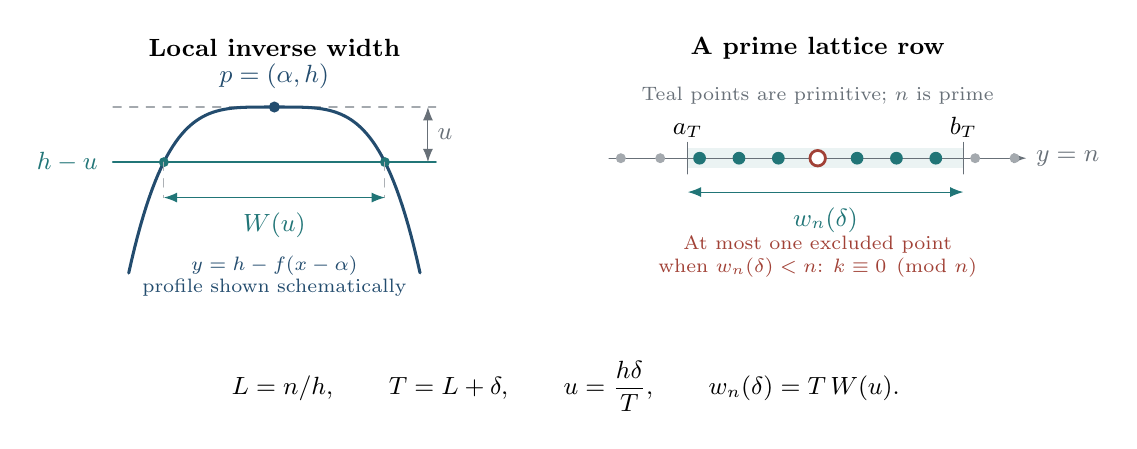
\begin{tikzpicture}[font=\small,>=Latex,line cap=round]
  \begin{scope}[shift={(-3.7,.3)}]
    \node[font=\bfseries\small] at (0,2.25) {Local inverse width};
    \draw[mpgray!60,dashed] (-2.05,1.5)--(2.05,1.5);
    \draw[mpblue,line width=1.1pt,domain=-1.85:1.85,samples=100]
      plot (\x,{1.5-.18*\x*\x*\x*\x});
    \draw[mpteal,line width=.8pt] (-2.05,.8)--(2.05,.8);
    \fill[mpblue] (0,1.5) circle (2pt) node[above=3pt] {$p=(\alpha,h)$};
    \fill[mpteal] (-1.404,.8) circle (1.8pt);
    \fill[mpteal] (1.404,.8) circle (1.8pt);
    \draw[mpgray!55,dashed] (-1.404,.8)--(-1.404,.35) (1.404,.8)--(1.404,.35);
    \draw[<->,mpteal] (-1.404,.35)--node[below=2pt] {$W(u)$}(1.404,.35);
    \draw[<->,mpgray] (1.95,.8)--node[right] {$u$}(1.95,1.5);
    \node[left=2pt,text=mpteal] at (-2.05,.8) {$h-u$};
    \node[text=mpblue,align=center,font=\scriptsize] at (0,-.65)
      {$y=h-f(x-\alpha)$\\profile shown schematically};
  \end{scope}
  \begin{scope}[shift={(3.2,1.15)}]
    \node[font=\bfseries\small] at (0,1.4) {A prime lattice row};
    \fill[mpteal!9] (-1.65,-.13) rectangle (1.85,.13);
    \draw[->,mpgray] (-2.65,0)--(2.65,0) node[right] {$y=n$};
    \foreach \x in {-2.5,-2,-1.5,-1,-.5,.5,1,1.5,2,2.5}
      \fill[mpgray!60] (\x,0) circle (1.8pt);
    \foreach \x in {-1.5,-1,-.5,.5,1,1.5}
      \fill[mpteal] (\x,0) circle (2.3pt);
    \filldraw[fill=white,draw=mpred,line width=1pt] (0,0) circle (2.8pt);
    \draw[mpgray] (-1.65,-.2)--(-1.65,.2) (1.85,-.2)--(1.85,.2);
    \node[above=4pt] at (-1.65,0) {$a_T$};\node[above=4pt] at (1.85,0) {$b_T$};
    \draw[<->,mpteal] (-1.65,-.43)--node[below=2pt] {$w_n(\delta)$}(1.85,-.43);
    \node[align=center,text=mpred,font=\scriptsize] at (0,-1.25)
      {At most one excluded point\\when $w_n(\delta)<n$: $k\equiv0\pmod n$};
    \node[font=\scriptsize,text=mpgray] at (0,.8) {Teal points are primitive; $n$ is prime};
  \end{scope}
  \node[align=center] at (0,-1.75)
    {$L=n/h,\qquad T=L+\delta,\qquad
      u=\displaystyle\frac{h\delta}{T},\qquad
      w_n(\delta)=T\,W(u)$.};
\end{tikzpicture}
\caption[A flat supporting cap and a primitive-row burst]{How a supporting cap becomes a primitive-row contribution.
At the contact scale $L=n/h$, the hypothesis $\alpha/h\notin\mathbb Q$
leaves the row empty. Increasing the scale to $T=L+\delta$ cuts an interval
of width $TW(h\delta/T)$ from that row. When $n$ is prime and the width
is smaller than $n$, all but at most one of its integer points are
primitive. The local profile and row spacing are schematic; the
displayed width relation is exact.}
\label{fig:mono-flat-row}
\end{figure}
% END INLINE FIGURE

\subsection{Model flatness profiles and what they do not determine}
\label{subsec:flatnessmodels}

For illustration, suppose the two-sided local graph satisfies
\[
 f(s)\leq C\exp\!\left(-\frac a{|s|^\beta}\right),
 \qquad a,\beta>0,
\]
for sufficiently small nonzero $s$. Then
\[
 W(u)\geq
 2\left(\frac a{\log(C/u)}\right)^{1/\beta},
\]
and~\eqref{eq:inverseflatmicroscopic} gives, along arbitrarily large
prime-row contact scales,
\begin{equation}
 \max\{|E_B(L)|,|E_B(L+L^{-1})|\}
 \gg_{B,a,\beta}\frac L{(\log L)^{1/\beta}}.
 \label{eq:exponentialflatrow}
\end{equation}
If the graph has matching upper and lower estimates of this form, the
row width itself has this order. This does not prove that the full
discrepancy has exactly this order; other rows and other supporting
directions can contribute.

Other infinitely flat local profiles give different slowly varying
factors. For example, the symmetric model
$f(s)=\exp[-\exp(|s|^{-\beta})]$ gives a row width of order
$L/(\log\log L)^{1/\beta}$. The model
\[
 f(s)=\exp[-(\log(1/|s|))^\gamma],\qquad\gamma>1,
\]
gives a width of order
\[
 L\exp[-(2\log L)^{1/\gamma}].
\]
These are convex for sufficiently small $|s|$ and illustrate local
possibilities. They are not asserted here to be the precise profiles
of a hyperbolic torus norm ball.

For a strictly convex body, $W(u)\to0$. Consequently the single-row
argument with a microscopic scale increment yields a quantity $o(L)$,
although it can exceed every fixed power $L^{1-\varepsilon}$.
It neither proves a literal $\Omega(L)$ lower bound nor distinguishes
an $O(L)$ global remainder from an $O(L\log L)$ remainder. Its role is
to quantify one geometric obstruction, rather than to identify the
entire sharp remainder.

\subsection{An exact row diagnostic and its precision requirements}
\label{subsec:rowdiagnostic}

For an arbitrary positive integer $n$ and a row interval $[a,b]$, the
primitive count is exactly
\begin{equation}
 \#\{k\in\ZZ\cap[a,b]:\gcd(k,n)=1\}
 =\sum_{d\mid n}\mu(d)
 \left(\left\lfloor\frac bd\right\rfloor
       -\left\lceil\frac ad\right\rceil+1\right).
 \label{eq:primitiveintervalexact}
\end{equation}
In particular, it equals
\[
 (b-a)\frac{\varphi(n)}n+O(2^{\omega(n)}).
\]
The formula includes endpoints exactly. For prime $n$ and $b-a<n$,
the simpler absolute-error comparison with $b-a$ used above applies.

One can therefore record the local statistic
\[
 J_n=P_{B,n}(n/h+h/n),\qquad
 P_{B,n}(T)=\#\{k\in\ZZ:\gcd(k,n)=1,\ (k,n)\in TB\},
\]
at prime $n$. Since $L=n/h$ and $h/n=L^{-1}$, the proposition gives
\[
 J_n=(L+L^{-1})W\!\left(\frac h{L^2+1}\right)+O(1).
\]
This statistic needs no estimate of $\operatorname{Area}(B)$; it tests
the local flatness mechanism directly. It does require a verified
lattice-rational supporting normal at an irrational radial point.
Finding such a direction is a separate geometric step and is not
automatic for an arbitrary fixed surface.

The height $h$ must also be known accurately. An error $\Delta h$ moves
the contact scale $n/h$ by approximately $-L\Delta h/h$. Resolving
the window of width $L^{-1}$ thus requires $|\Delta h|\ll hL^{-2}$.
Using a larger window relaxes this requirement but changes the depth
sampled by~\eqref{eq:inverseflatwidth} and increases the background
main-term increment. The local statistic is consequently complementary
to a global main-term-free discrepancy diagnostic; it does not replace
one.



\subsection{A trace diagnostic: retained report and bounded replacement}
\label{subsec:torustraceexperiment}

The count here is $N_X(L)$ for unoriented essential simple closed
geodesics on a once-punctured torus, with the convention
$N_X(L)=\#\{\gamma:\ell_\gamma\le L\}$. Each primitive pair
$(p,q)\in\mathbb Z^2$ is identified with $(-p,-q)$, so this is half
the signed primitive-vector count for the corresponding norm ball.
A positive trace triple satisfies
\[
 x^2+y^2+z^2=xyz,\qquad x,y,z>2,
\]
and a Farey edge replaces $z$ by $xy-z$. The identification of Farey
regions with simple curves and this edge relation are described in
\cite[Sections~1--2]{BowditchMarkoff}. For the experiment take the reduced
triples
\begin{equation}
 (x,y,z)=(3,3,3),\qquad
 (x,y,z)=\left(\frac52,\frac{10-\sqrt{11}}2,4\right).
 \label{eq:diagnostictracetriples}
\end{equation}
The first is the modular torus; the second is an asymmetric example.
Both satisfy $2<x\le y\le z\le xy/2$.

Assign the root curves the slopes $(1,0)$, $(0,1)$, and $(1,1)$,
respectively. The three open sectors between these roots enumerate
every other unoriented primitive slope once by Farey mediants. In the
negative-slope sector use the signed endpoints $(1,0),(0,-1)$;
the other two sectors have endpoints $(1,0),(1,1)$ and
$(0,1),(1,1)$. Canonical representatives have $q>0$, with $(1,0)$
as the only representative at infinity. Sector endpoints are counted
only as roots. After introducing an outward
trace $c\ge\max(a,b)>2$, the two new traces are $ac-b$ and $bc-a$,
both strictly larger than $c$. Therefore pruning a sector when its new
curve exceeds the cutoff does not omit shorter descendants. Equal traces
are retained with their curve multiplicities; they are not deduplicated.
The hyperbolic length associated with trace $x$ is $2\arcosh(x/2)$.

To avoid overflow the computation uses logarithmic traces. If
$u_a=\log a$, $u_b=\log b$, and $u_c=\log c$, then
\[
 \log(ab-c)=u_a+u_b+
        \log\bigl(1-\exp(u_c-u_a-u_b)\bigr).
\]
On the chosen outward edges the subtracted ratio is at most $1/2$,
so this computation avoids catastrophic cancellation. The supplied draft
describes extended-precision arithmetic for this recursion and double
precision for sorting the resulting lengths. That reported implementation
was not included in the supplied materials. The bounded replacement below
uses binary64 logarithmic recursion and a separate exact-trace oracle.
Neither calculation provides an interval certificate of every event location.

\paragraph{Retained numerical report, awaiting reproduction.}
The supplied draft reports enumeration through hyperbolic length $8192$, obtaining
$18\,191\,508$ curves for the modular torus and $18\,486\,116$ for
the asymmetric torus. Such a cutoff permits evaluating the dyadic block statistics
through $T=2048$, because the largest count used in a block is $N_X(4T)$.
The following selected values are retained verbatim from that report;
all entries are rounded and have not been reproduced for this edition.

\begin{center}
\begin{tabular}{r r r r r}
\toprule
&\multicolumn{2}{c}{Modular torus}&\multicolumn{2}{c}{Asymmetric torus}\\
$T$&$M(T)$&$Q(T)$&$M(T)$&$Q(T)$\\
\midrule
32 & 2.1686 & 0.6015 & 0.8134 & 0.2734 \\
128 & 1.1130 & 0.3501 & 0.5285 & 0.1494 \\
512 & 0.7415 & 0.1697 & 0.3756 & 0.0950 \\
2048 & 0.4342 & 0.0950 & 0.2492 & 0.0612 \\
\bottomrule
\end{tabular}
\end{center}

According to the supplied draft, the reported maxima use all computed
length events, including the half-length events, rather than an integer
mesh. It reports that an independent direct-trace computation at $100$
decimal digits reproduces
all lengths through $64$ within $3.6\times10^{-15}$, and thirty
selected long recursion paths reaching lengths near $8192$ agree within
$7.5\times10^{-13}$. The latter include long repeated-twist paths.
The same report states that every dyadic cutoff used for the integer counts is separated from the
computed spectrum by at least $8.3\times10^{-5}$.

It also describes a separate sensitivity calculation treating nearby events as having an
unknown internal order and allows errors up to $10^{-6}$ in each event
position. Over all blocks the resulting lower and upper bounds for
$M(T)$ differ by less than $7.1\times10^{-7}$. This is a conditional
sensitivity check, not a proof that every computed length has that error
bound. The advertised source, full block table, precision report, and
sensitivity tables were not found in the supplied archive or repositories.
Consequently these counts, table entries, precision comparisons, and
sensitivity bounds remain unreplayed reported results. This edition does
not claim that the advertised diagnostic archive accompanies the book.

The displayed finite-range normalized excursions decrease overall;
they do not establish an asymptotic linear or sublinear bound. The modular
torus was already singled out as a candidate for exceptional behavior in
\cite[Conjecture~4.3]{McShaneRivinTori}. Neither example is asserted to
have a verified lattice-rational supporting normal at an infinitely flat
irrational point. Sparse resonances can occur beyond the tested range.
The stability claims for this reported long run remain awaiting their
computational evidence.

\paragraph{A bounded replacement calculation.}
The maintained recipe \path{experiments/section30/run.py} performs a new
calculation through length $64$ for the same two exact trace triples.
It finds $1104$ modular and $1127$ asymmetric curves. This is a replacement
experiment, not a reconstruction of the missing length-$8192$ run.
Its complete slope list, exact traces, numerical lengths, and block
statistics are recorded in \path{artifacts/section30/result.json}, with
the source identity and precision settings. The new block values are
\begin{center}
\begin{tabular}{r r r r r}
\toprule
&\multicolumn{2}{c}{Modular torus}&\multicolumn{2}{c}{Asymmetric torus}\\
$T$&$M(T)$&$Q(T)$&$M(T)$&$Q(T)$\\
\midrule
4 & 3.3289 & 1.4538 & 1.4983 & 0.7563 \\
8 & 3.2433 & 1.2476 & 1.2352 & 0.4951 \\
16 & 2.0238 & 0.8521 & 1.2246 & 0.3942 \\
\bottomrule
\end{tabular}
\end{center}

The check uses two enumerations. The first traverses the three sectors
with logarithmic traces. The second evaluates exact trace polynomials
for all primitive slopes in the box $|p|\le160$, $0\le q\le160$,
using Euclidean Farey parents, without length-based pruning. This box
suffices for these two fixtures: put $v=\log(\operatorname{tr}/2)$.
The outward subtraction bound gives $v_c\ge v_a+v_b$, and each root
has $v\ge\log(5/4)>1/5$. The corresponding sector weight is
$F=|p|+q$ for $p<0$, $F=p$ for $p\ge q\ge0$, and $F=q$ for
$q\ge p\ge0$. Thus $F\ge\max(|p|,q)$ and
\[
 \ell=2\arcosh(e^v)>2v\ge\frac25F.
\]
Every curve of length at most $64$ therefore lies in the stated box.
There are $31\,224$ primitive unoriented slopes in that box, including
$(1,0)$. Equal traces retain all their distinct slopes.

The oracle uses rational arithmetic in $\mathbb Q(\sqrt{11})$ for
traces and evaluates lengths at $100$ and $140$ decimal digits.
Opposite-signed algebraic coefficients are evaluated through the exact
norm and the conjugate denominator to avoid subtractive cancellation.
Both precisions select the same slopes as the logarithmic traversal;
the length comparisons differ by less than $1.1\times10^{-98}$ between
the two decimal precisions and by less than $1.1\times10^{-13}$ from
the binary64 logarithmic calculation. These are observed residuals,
not rigorous error enclosures.

The displayed metrics use the oracle lengths rounded to binary64.
An event sweep is compared with direct counts on every event interval,
including one-sided limits and simultaneous jumps. Comparing metrics
from the logarithmic and exact-trace length calculations gives differences
below $2.7\times10^{-15}$ for $M$ and $3.2\times10^{-15}$ for $Q$.
The recipe also supplies conservative rational bounds for $M$, conditional
on each stored length having error at most $10^{-10}$; it does not
certify that error hypothesis. These bounds concern the fixed supplied
curve list; application to the complete spectrum also assumes that no
omitted curve can enter a block threshold under the perturbation.
The full derivation and run instructions
are in \path{experiments/section30/README.md}. This bounded check provides
no long-range sensitivity bound, no asymptotic remainder theorem, and
no audit of the remaining proof chain in this section.

\subsection{A recent qualification of irrational flatness}
\label{subsec:recentflatnessqualification}

Doan--Li--Nguyen's recent preprint~\cite{DoanLiNguyenStableNorm},
version~3 dated 9 October 2026, gives a Diophantine refinement of the
irrational flatness statement. Its Theorem~4.7 states that infinite
graph-flatness holds precisely when the exponential rational-approximation
exponent vanishes; superexponentially approximable irrational directions
can have graph-flatness order only one. In slope coordinates the relevant
quantity is $\limsup_j(\log q_{j+1})/q_j$, where $q_j$ are continued-fraction
denominators. The local convexity mechanism is that a nearby rational
corner can remain visible at a much smaller spatial scale than its
exponentially small angle.

We have checked the local Fricke and convexity mechanism relevant to
this distinction, but have not audited the entire preprint. None of its
global counting assertions is used in the proofs above. In particular,
Propositions~\ref{prop:normballflatrow} and~\ref{prop:inverseflatrow}
retain their explicit flat-point hypotheses, and
Proposition~\ref{prop:strictconvexlittleo} uses only strict convexity.
The preprint also continues to list the McShane--Rivin $O_X(L\log L)$
bound as the cumulative counting benchmark; its multiplicity estimate
concerns exact length levels, a different question.



\section{Arithmetic cancellation and the geometric remainder}
\label{sec:arithmeticgeometry}

\subsection{A transfer estimate with both inputs explicit}
\label{subsec:primitiveRHtransfer}

Let $B\subset\mathbb R^2$ be a fixed convex body containing the origin in
its interior, and normalize its gauge so that the shortest nonzero
integer vector has gauge one.  Put
\[
 A_B(u)=\#\bigl(uB\cap(\mathbb Z^2\setminus\{0\})\bigr),\qquad
 \Delta_B(u)=A_B(u)-a_Bu^2,\qquad a_B=\operatorname{Area}(B),
\]
and write
\[
 P_B(L)=\#\bigl(LB\cap\mathbb Z^2_{\rm prim}\bigr),\qquad
 E_B(L)=P_B(L)-\frac{a_B}{\zeta(2)}L^2.
\]
All primitive vectors are counted with their signs; an unoriented count
for a centrally symmetric body is half this count.
The notation $\Delta_B$ here is the all-point discrepancy $D_B$ of
Section~\ref{subsec:mobiusmodulus}.

There are two inputs in the primitive problem: the geometric discrepancy
$\Delta_B$, and cancellation in the M\"obius function.  A quantitative
bound for the second input does not by itself specify the first.  The
following elementary estimate keeps their roles separate.

\begin{proposition}[A large-divisor transfer estimate]
\label{prop:primitiveRHtransfer}
Suppose
\[
 M(x):=\sum_{n\le x}\mu(n),\qquad |M(x)|\le Cx\eta(x),
\]
where $\eta$ is nonnegative and nonincreasing on $[1,\infty)$.
Then, for every integer $1\le D\le L$,
\begin{equation}\label{eq:primitiveRHmaster}
 |E_B(L)|\ll_{B,C}
       \sum_{d\le D}|\Delta_B(L/d)|
       +\frac{L^2}{D}\eta(D).
\end{equation}
In particular, $M(x)\ll x^\theta$, with $0\le\theta<1$, gives
\begin{equation}\label{eq:primitiveRHpowerM}
 |E_B(L)|\ll_{B,\theta}
       \sum_{d\le D}|\Delta_B(L/d)|+L^2D^{\theta-2}.
\end{equation}
\end{proposition}

\begin{proof}
M\"obius inversion gives
\[
 P_B(L)=\sum_{d\le L}\mu(d)A_B(L/d).
\]
Set $U=L/D$.  Reversing the order of summation in its large-divisor
part gives the exact identity
\[
 \sum_{d>D}\mu(d)A_B(L/d)
   =\sum_{\substack{m\in\mathbb Z^2\setminus\{0\}\\\|m\|_B\le U}}
       \left(M\!\left(\frac{L}{\|m\|_B}\right)-M(D)\right).
\]
The summands with $\lfloor L/\|m\|_B\rfloor=D$ are zero.
Since $A_B(u)\ll_B u^2$ for $u\ge1$, partial summation gives
\[
 \sum_{\substack{m\ne0\\\|m\|_B\le U}}\|m\|_B^{-1}\ll_B U.
\]
Monotonicity of $\eta$ therefore bounds the large-divisor part by
\[
 \eta(D)\left(L\sum_{0<\|m\|_B\le U}\|m\|_B^{-1}
                      +D A_B(U)\right)
       \ll_B\frac{L^2}{D}\eta(D).
\]
The area term has the same tail bound, because partial summation yields
\[
 \left|\sum_{d>D}\frac{\mu(d)}{d^2}\right|
       \ll\frac{\eta(D)}{D}.
\]
Subtract the area main term in the small-divisor sum and bound its
remaining terms absolutely.  This proves the first estimate; take
$\eta(x)=x^{\theta-1}$ for the second.
\end{proof}

\subsection{An unconditional sublinear consequence of the Dini condition}
Define the nonincreasing geometric modulus
\[
 \omega_B(u)=\sup_{v\ge u}\frac{|\Delta_B(v)|}{v}.
\]
For $L/(D+1)\ge1$, direct comparison on the intervals
$[L/(d+1),L/d]$ gives
\begin{equation}\label{eq:primitiveRHmodulus}
 \sum_{d\le D}|\Delta_B(L/d)|
   \le 2L\int_{L/(D+1)}^L\omega_B(u)\frac{du}{u}.
\end{equation}
Consequently,
\begin{equation}\label{eq:primitiveDiniPNT}
 \int_1^\infty\omega_B(u)\frac{du}{u}<\infty
 \quad\Longrightarrow\quad E_B(L)=o_B(L).
\end{equation}
Here the arithmetic input is only the prime number theorem, in the
equivalent form $M(x)=o(x)$, not RH.  Indeed, use the nonincreasing
envelope $\eta(x)=\sup_{y\ge x}|M(y)|/y$, fix $U\ge2$, and choose
$D=\lfloor L/U\rfloor$.  After division by $L$, the large-divisor
bound tends to zero for this fixed $U$, whereas the small-divisor bound
is at most
$2\int_{U/2}^{\infty}\omega_B(u)\,du/u$ for all sufficiently large $L$.
Let $L\to\infty$ and then $U\to\infty$.
This strengthens the earlier absolute-value Dini argument, which gave
only $O_B(L)$.


\subsection{Fixed zero-free half-planes and the recent quasi-RH claims}
\label{subsec:quasiRHapplication}

For the Riemann zeta function and $1/2\le\theta_0<1$, the standard
zero-free-half-plane formulation is equivalent to
\begin{equation}
 \zeta(s)\ne0\quad(\Re s>\theta_0)
 \quad\Longleftrightarrow\quad
 M(x)=O_\varepsilon(x^{\theta_0+\varepsilon})
 \quad\hbox{for every }\varepsilon>0.
 \label{eq:zeroFreeMertens}
\end{equation}
Here nonvanishing excludes the pole at $s=1$, where $1/\zeta$
instead has a zero. We give the analytic step because a fixed zero-free
half-plane and a height-dependent zero-free region are different inputs.

Suppose first that the left side of~\eqref{eq:zeroFreeMertens} holds.
Fix $0<\delta<(1-\theta_0)/2$. At sufficiently large $|t|$, choose the
branch of $\log\zeta$ on the disk centered at $2+it$ of radius
$R_2=2-\theta_0-\delta/4$ that agrees with the Euler-product logarithm
at its center. This disk contains neither zeros nor the pole.
Polynomial growth of $\zeta$ in a fixed vertical strip gives
$\Re\log\zeta\ll_\delta\log(2+|t|)$ there.
Borel--Carath\'eodory bounds $|\log\zeta|$ by the same order on the
smaller disk of radius $R=2-\theta_0-\delta/2$. On the disk of radius
$r_0=1/2$ the absolutely convergent Euler-product logarithm is bounded.
The three-circles theorem, with $r=2-\theta_0-\delta<R$, now gives
\[
 |\log\zeta(\sigma+it)|\ll_\delta(\log(2+|t|))^{\lambda_\delta},
 \qquad \theta_0+\delta\le\sigma\le2,\qquad
 \lambda_\delta=\frac{\log(r/r_0)}{\log(R/r_0)}<1.
\]
Consequently, for every $\varepsilon>0$,
$1/\zeta(\sigma+it)\ll_{\delta,\varepsilon}(1+|t|)^\varepsilon$
on $\sigma\ge\theta_0+\delta$; bounded heights and $\sigma\ge2$
are handled by analyticity of the reciprocal and the Euler product.

For a half-integer $x$, truncated Perron inversion on
$c=1+1/\log x$, at height $T=x^2$, has error
$O(x\log^2x/T)$ because $|\mu(n)|\le1$. Move the contour to
$\sigma_0=\theta_0+\delta$. There are no poles of the reciprocal in
the intervening strip. The new vertical integral is
$O_{\delta,\varepsilon}(x^{\sigma_0}T^\varepsilon)$ and the two
horizontal integrals are $O_{\delta,\varepsilon}(xT^{\varepsilon-1})$.
Choosing $\delta$ and $\varepsilon$ sufficiently small gives every
exponent $\theta_0+\varepsilon'$ requested on the right side
of~\eqref{eq:zeroFreeMertens}. Half-integers suffice since $M$ is
constant between consecutive integers.

Conversely, for each compact subset of $\Re s>\theta_0$, choose
$\varepsilon>0$ smaller than its distance from the boundary. The bound
for $M$ makes $s\int_1^\infty M(x)x^{-s-1}\,dx$ locally uniformly
convergent and holomorphic there. Partial summation identifies it with
$1/\zeta(s)$ on $\Re s>1$, so analytic continuation precludes a zero
of $\zeta$ in $\Re s>\theta_0$. This equivalence uses the Euler product,
meromorphic continuation and vertical growth of $\zeta$; zero-freeness
of an arbitrary Dirichlet series would not alone suffice.

The OpenAI manuscript dated 30 September 2026 claims the half-plane
$\Re s>7/8$ for all finite-order Hecke $L$-functions over
$\mathbb Q(\sqrt{-3})$, and hence for Dirichlet $L$-functions,
including $\zeta$~\cite[Theorem~1.1]{OpenAIQuasiRHSeptember}.
The manuscript dated 5 October 2026 gives a separate proof claiming
$\Re s>11/12$ and describes it as a simpler intermediate result toward
the September theorem~\cite[Theorem~1.1 and the following paragraph]{OpenAIQuasiRHOctober}.
For both papers we use the theorem statements in the TeX sources at
repository revision \texttt{adc7f1241b42} (the initial release), as pinned
in the claim ledger and bibliography. We checked those statements,
not either complete proof or its formalization. All applications here are conditional on
the explicit arithmetic hypothesis in Proposition~\ref{prop:primitiveRHtransfer}.
The corresponding Mertens exponents would be $7/8+\varepsilon$,
$11/12+\varepsilon$, and, under full RH, $1/2+\varepsilon$.
The generalized assertions about other $L$-functions are unnecessary
for this primitive planar count.

\subsection{Logarithmic geometric savings}
The next comparison is conditional on an additional estimate for the
all-point discrepancy:
\begin{equation}\label{eq:primitiveRHgeometry}
 |\Delta_B(u)|\ll_B\frac{u}{(\log u)^\beta},\qquad u\ge3,
 \qquad\beta>0.
\end{equation}
No such estimate is asserted here for a McShane--Rivin norm ball.

First suppose $M(x)\ll x^\theta$ for some fixed $\theta<1$.
Choose any fixed $d$ with
$1/(2-\theta)<d<1$, and take $D=\lfloor L^d\rfloor$.
The large-divisor contribution in~\eqref{eq:primitiveRHpowerM} is
$O(L^{2-d(2-\theta)})$, with exponent strictly smaller than one.
The small-divisor contribution is
\[
 \ll L\int_{L^{1-d}/2}^L\frac{du}{u(\log u)^\beta}
 \ll_{\beta,d} L(\log L)^{1-\beta}.
\]
Thus
\begin{equation}\label{eq:primitiveRHlogresult}
 M(x)\ll x^\theta\ (\theta<1),\quad
 \Delta_B(u)\ll u(\log u)^{-\beta}
 \quad\Longrightarrow\quad
 E_B(L)\ll L(\log L)^{1-\beta}.
\end{equation}
In particular, the geometric threshold $\beta=1$ gives $O_B(L)$.
Any fixed power saving for $M$ suffices for this conclusion: full RH
does not improve the logarithmic exponent in this elementary argument.

For comparison, the classical unconditional Vinogradov--Korobov estimate,
recorded for example in Zhai~\cite[eq.~(1.5)]{ZhaiPrimitive2003}, has the form
\[
 M(x)\ll x\exp\!\left(-c(\log x)^{3/5}
                              (\log\log x)^{-1/5}\right).
\]
Write $F(L)=(\log L)^{3/5}(\log\log L)^{-1/5}$ and take
$D=\lfloor L\exp(-aF(L))\rfloor$ with a sufficiently small fixed
$a>0$.  Since $F(D)\sim F(L)$, the large-divisor part is
$O(L\exp(-c'F(L)))$.  The small-divisor part is bounded by
\[
 L\int_{\exp(aF(L))/2}^L\frac{du}{u(\log u)^\beta}.
\]
The resulting elementary comparison is
\[
\begin{array}{c|c|c}
 \text{geometric exponent }\beta
 &\text{unconditional VK input}
 &M(x)\ll x^\theta,\ \theta<1\\ \hline
 0<\beta<1
 &O\!\left(L(\log L)^{1-\beta}\right)
 &O\!\left(L(\log L)^{1-\beta}\right)\\[2pt]
 \beta=1
 &O(L\log\log L)
 &O(L)\\[2pt]
 \beta>1
 &O\!\left(LF(L)^{1-\beta}\right)
 &O\!\left(L(\log L)^{1-\beta}\right).
\end{array}
\]
These are consequences of one elementary splitting argument, not
assertions of optimality.  The constants can depend on $B$, $\beta$,
the arithmetic exponent, and the chosen cutoff exponent.

\subsection{Power-saving geometric discrepancies and established benchmarks}
If instead $|\Delta_B(u)|\ll u^\alpha$ with $0\le\alpha<1$, then
\[
 \sum_{d\le D}|\Delta_B(L/d)|\ll L^\alpha D^{1-\alpha}.
\]
Balancing this with $L^2D^{\theta-2}$ gives
\begin{equation}\label{eq:primitiveRHbalancedpower}
 D\asymp L^{(2-\alpha)/(3-\alpha-\theta)},\qquad
 E_B(L)\ll L^{\kappa(\alpha,\theta)},\qquad
 \kappa(\alpha,\theta)=\frac{2-\alpha\theta}{3-\alpha-\theta}.
\end{equation}
For example, $\alpha=2/3$ and a Mertens exponent arbitrarily close
to $1/2$ give $O_\varepsilon(L^{10/11+\varepsilon})$.
Exponents arbitrarily close to $7/8$ and $11/12$ give, respectively,
$O_\varepsilon(L^{34/35+\varepsilon})$ and
$O_\varepsilon(L^{50/51+\varepsilon})$ by this method.
These examples concern a hypothetical or separately established
geometric estimate with $\alpha=2/3$; they do not assign that exponent
to a McShane--Rivin ball.  Stronger results for smooth curved domains
use additional structure and should not be confused with this general
transfer bound.

With the same power-saving geometric input, the unconditional VK
estimate already gives
\[
 E_B(L)\ll L\exp(-c_B F(L))
\]
for some $c_B>0$, by choosing
$D=L\exp(-aF(L))$ and balancing the two exponential factors.
Thus sublinear primitive errors in suitable geometries do not require RH.


This unconditional sublinear conclusion is a classical one for
sufficiently smooth, positively curved domains: Zhai records it in
equation~(1.4) of~\cite{ZhaiPrimitive2003}. His parameter is the area
scale $x=L^2$, so his $O(x^{1/2}\exp(-cF(x)))$ becomes
$O(L\exp(-c'F(L)))$ here. The hypotheses include finite nonzero
curvature throughout and a $C^4$ Gauss map. Those hypotheses do not
hold for a McShane--Rivin ball.

Under RH, Baker~\cite[Theorem~1]{BakerPrimitive2010} proves
$O_\varepsilon(L^{10/13+\varepsilon})$ for a specified class of
piecewise $C^4$ domains whose arcs have nonzero curvature, with
additional $C^4$ reciprocal-curve regularity and rational endpoint
tangents, as specified by hypotheses (H1)--(H4) on pages~267--268.
This is an established comparison result, not a claim about the best
current exponent or about the flat norm balls considered here.
In the opposite direction, the unconditional polygon obstruction
$\Omega_\pm(L\sqrt{\log\log L})$ recalled in
Section~\ref{subsec:rationalpolygonbenchmark} persists regardless of RH.
It belongs to rational polygons and is not a lower bound for strictly
convex bodies. These examples show why the shape hypothesis must
accompany any arithmetic hypothesis.

\subsection{The remaining geometric obstruction}
Strict convexity supplies $\Delta_B(u)=o(u)$ and hence
$\omega_B(u)\to0$, but no specified rate for that convergence.
Under any fixed arithmetic exponent $\theta<1$, the preceding
power cutoff yields a bound of the form
\[
 |E_B(L)|\ll L\log L\,\omega_B(cL^{1-d})
                      +L^{2-d(2-\theta)}.
\]
It is again $o(L\log L)$, without a universal logarithmic saving
specified by this argument.  This is a limitation of the stated inputs
and this transfer estimate, not an impossibility theorem for more
special convex bodies.

One cannot simply multiply a bound for $M$ by the supremum of the
weights $\Delta_B(L/d)$.  Abel summation also sees their variation.
On a dyadic interval $d\asymp D$, the counting part of these weights
can have total variation of order $(L/D)^2$, despite a much smaller
pointwise discrepancy.  The large-divisor estimate above pays for
that variation explicitly.  Further cancellation would require
additional information about the geometric weights or their correlation
with $\mu(d)$.

Equivalently, for $\Re s>2$ the gauge zeta functions satisfy
\[
 Z_B(s)=\sum_{m\ne0}\|m\|_B^{-s},\qquad
 Z_B^{\rm prim}(s)=\frac{Z_B(s)}{\zeta(s)}.
\]
The estimate $\Delta_B(u)=o(u)$ provides the representation
\[
 Z_B(s)=\frac{a_Bs}{s-2}
          +s\int_1^\infty\Delta_B(u)u^{-s-1}\,du,
 \qquad \Re s>1.
\]
A zero-free result for the denominator does not on its own continue
the geometric numerator through the line $\Re s=1$, nor provide the
vertical growth bounds needed for a sharp counting inversion.  This is
the analytic reason to keep the arithmetic and geometric inputs separate.


For a body satisfying the infinite-flatness and rational-normal hypotheses
of Proposition~\ref{prop:normballflatrow}, the prime-row construction gives
$\Omega(L^{1-\varepsilon})$ along an unbounded sequence for every
$\varepsilon>0$. This excludes a fixed sublinear power bound for that
body even if RH holds. It does not exclude $O(L)$, or even $o(L)$:
the quantitative lower bound is $L W(h/L^2)$ up to constants, and
$W(h/L^2)\to0$ under strict convexity. A useful next geometric target is therefore a quantitative modulus.
One possible target is $\Delta_B(u)=O(u/\log u)$, provided it is
compatible with that body's local widths. Under the same supporting-row,
two-sided-graph and irrational-contact hypotheses, the row is empty at
$L=n/h$ and contributes $w_n(L^{-1})+O(1)$ all points at $L+L^{-1}$.
The all-point main term changes by only $a_B(2+L^{-2})$, so
\[
 \max\{|\Delta_B(L)|,|\Delta_B(L+L^{-1})|\}
 \ge \frac L2W(h/L^2)-O_B(1).
\]
There is no totient density factor in this all-point estimate, and it
holds for every sufficiently large integer $n$, without primality.
Consequently the proposed target requires $W(h/L^2)=O(1/\log L)$
along these contact scales. Strict
convexity and infinite flatness alone do not give that condition;
the model $f(s)=\exp[-\exp(|s|^{-\beta})]$ in
Section~\ref{subsec:flatnessmodels} violates it. Establishing a compatible
modulus for any specified McShane--Rivin ball remains a separate problem.

The all-point target has a numerical diagnostic independent of the area
constant, just as in Section~\ref{subsec:dyadicdiagnostic}. Define
\[
 \mathcal D_A(L)=A_B(2L)-4A_B(L).
\]
The dyadic inverse identity proves the equivalence
\begin{equation}
 \Delta_B(L)=O(L/\log L)
 \quad\Longleftrightarrow\quad
 \mathcal D_A(L)=O(L/\log L).
 \label{eq:allPointLogDiagnostic}
\end{equation}
Indeed, the reverse implication follows from
$\Delta_B(L)=-\sum_{j\ge0}4^{-j-1}\mathcal D_A(2^jL)$
and $\log(2^jL)\ge\log L$. For a symmetric torus norm ball,
let $\lambda_\gamma$ be the simple-geodesic length in the same
normalization as the gauge of $B$. The length list already used in
Section~\ref{subsec:torustraceexperiment}, rescaled when imposing the
unit-shortest-vector convention, gives the exact identity
\[
 A_B(L)=2\sum_{\substack{\gamma\text{ unoriented simple}\\\lambda_\gamma\le L}}
               \left\lfloor\frac L{\lambda_\gamma}\right\rfloor.
\]
Thus the proposed geometric threshold can be investigated without
estimating the norm-ball area or introducing a new enumeration of
curve types. No finite numerical range proves the uniform bound
in~\eqref{eq:allPointLogDiagnostic}.

The full campaign \path{experiments/torus_campaign/run.py} implements
this signed-multiple diagnostic at its dyadic cutoffs, with the all-point
rows and differences in \path{artifacts/torus_campaign/result.json}.
The floor comparisons use exact rational representations of the stored
binary64 lengths. Membership for the true geodesic lengths remains
numerical; the exact identity does not certify the required length or
completeness assumptions. The campaign uses hyperbolic lengths
$\ell_\gamma$ without rescaling. If
$s_X$ is the shortest hyperbolic length, the unit-shortest-vector gauge
uses $\lambda_\gamma=\ell_\gamma/s_X$ and hence
$A_B(L)=A_{\rm hyp}(s_XL)$. The campaign's hyperbolic dyadic rows must
be interpreted with that change of units; they do not establish a
uniform logarithmic bound. The separate finite companion
\path{experiments/counting_mixing/run.py} checks rational examples of
M\"obius inversion, signed multiples, row selectors, finite dyadic
identities and conditional balance exponents. These finite checks do
not supply either the required geometric modulus or an arithmetic
hypothesis. Source, independent-review and generation records are in
\path{docs/execution/counting-mixing-review-2026-11-01/}.


\monographpart{Open problems and conjectural directions}{The comparisons suggest concrete further estimates, integrations, and gluing problems. Their hypotheses identify what the next results would need to establish.}

\section{Questions suggested by the calculations}
\label{sec:questions}

The ideal volume proposal already has an established measure-theoretic
realization in~\eqref{eq:polyhedralpartition}, and the tree methods described
in Section~\ref{sec:hyperideal} also compute bordered genus-zero volumes.
The following questions isolate further work suggested by the discussion;
they are proposed tasks, not claims that no related results exist.

\begin{question}[Direct hyperideal integration]
Can the fixed-$L$ domains and the density~\eqref{eq:hyperidealdensity} be
integrated directly, with all cell and symmetry factors, to recover
$2\pi^2+\frac12\sum_iL_i^2$? Which change of variables makes the
cancellation or polynomiality visible?
\end{question}

\begin{question}[A usable measure on general polyhedral cells]
Can~\eqref{eq:pfaffiandensity} be expressed in dihedral-angle variables in
a way that makes higher-dimensional cell integrals computationally useful?
In the ideal case the measure is particularly simple. What replaces that
simplicity for fixed hyperideal boundary lengths or compact cone openings?
\end{question}

\begin{question}[Gluing and topology]
Can a polyhedral description be combined with Fenchel--Nielsen gluing to
give a practical calculation for arbitrary $(g,n)$? A proposed formula
must specify both the cutting multiplicity and the full mapping-class
quotient; integrating over all pants lengths and twist periods alone
overcounts moduli space.
\end{question}

\begin{question}[Curvature corrections in period coordinates]
Can the correction class $\Xi_\mu$ in~\eqref{eq:Xiclass} be represented
by an explicit first curvature correction to the WP form in
the actual finite-area conformal coordinates? Equation~\eqref{eq:Frickefirstcorrection}
answers the local four-point calculation in a blown-up character chart,
whose conversion to conformal coordinates is still required.
How does the local density behave
in a joint limit toward a balanced collision wall, where the
final-chamber expansion is not uniform in the weights?
\end{question}

\begin{question}[Beyond the regular quantum degeneration]
Can Proposition~\ref{prop:regularquantumAiry} be extended uniformly
over compact sets of nondegenerate Euclidean tetrahedral shapes,
with a geometric description of the required scalar normalization?
Can a geometric state
integral in that regime produce the Thurston--Deligne--Mostow measure
on the boundary-shape space? The model~\eqref{eq:modelpartition}
specifies a classical comparison, not an identification with an
existing quantum invariant. The exact Liouville
identity~\eqref{eq:exactLiouvillecurvature} and the torsion
limit~\eqref{eq:torsionDMlimit} identify two precise boundary
constructions; the auxiliary-tetrahedron obstruction and the
different regimes in~\eqref{eq:areaLiouvillecharge} explain
what remains to connect them to that joint asymptotic.
The finite one-screening fusion calculation in
Section~\ref{sec:screenedfusion} computes the finite period and
residue-sector comparison, with a logarithmic limit at balanced
weights. Its direct infinite-spectral derivation uses the
continuation and tail-control input~\eqref{eq:screeningtailinput};
Section~\ref{sec:normalizedsixj} fixes the quantum-group
normalization, proves the rank-two obstruction, and computes
the classical rank-three fold in the regular compact model.
Section~\ref{sec:quantumAiry} corrects the integration-coordinate
dictionary, removes the external parameter poles, and proves the
uniform regular-family Airy formula with its first correction.
General shape dependence, global gluing, and identification of
the resulting measure remain to be established.
\end{question}

\begin{question}[Uniform quantum Dehn filling]
For a knot complement admitting the positive geometric optimization
of Section~\ref{sec:dehnresponse}, can an exact quantum surgery
representation be controlled uniformly in a complex neighborhood
of complete peripheral holonomy, with a nonzero geometric contribution
and bounds on all competing terms? Proposition~\ref{prop:dehncriticalvalue}
already fixes every classical long-slope coefficient, and
\eqref{eq:dehngaussiantorsion} specifies the torsion check. The further
issue is the analytic input of
Proposition~\ref{prop:dehnquantumconditional}, especially in a joint
limit where the slope varies with the quantum level.
\end{question}


\begin{question}[Certified realization and quantitative angle bounds]
For the planar problem of Section~\ref{sec:ipolybridge}, can positive
feasibility, initial centering, inexact solves, and geometric error
certification be combined into a complete complexity theorem with
explicit input and precision dependence? For a three-manifold angle
polytope whose maximum is interior, which additional geometric hypotheses
bound its smallest angle in terms of the combinatorial input and a
quantitative feasible margin? The barrier iteration bound is available;
the planar Laplacian sign structure does not extend automatically to
the full three-dimensional Hessian.
\end{question}

\begin{question}[A continuum comparison of second variations]
Can a family of refined polyhedral functionals, with specified geometric
convergence and normalization, have a second-variation limit related to
a WP potential? The exact cotangent identity, Schur complement, and
Gaussian determinant in Section~\ref{sec:ipolybridge} provide discrete
objects for such a comparison. Control of their limits and an explicit
identification of the target metric are still required.
\end{question}

\begin{question}[Continuation of a coefficient Laplace transform]
Does $D_C(s)$ from Section~\ref{sec:coefficientdistributions} admit a
meromorphic continuation beyond the proved half-plane $\Re s>1$?
A proof must control coefficient extraction in the continued
character-valued expression, since it is not bounded for the
uniform norm on unitary characters.
\end{question}

\begin{question}[Control of the globally filtered remainder]
Proposition~\ref{prop:globalonecrossing} gives a bounded global
cancellation of every one-crossing primitive and all its iterates.
Can the signed residual $\mathcal R_X$ in~\eqref{eq:globalresidual}
be estimated with constants controlled by the geometry of $X$?
The exact obstruction~\eqref{eq:globalobstruction} rules out a
perfect fixed linear selector; length-dependent cancellation or
the nonlinear diagonal extraction in~\eqref{eq:globaldiagonal}
retains information that such a selector discards.
\end{question}

\begin{question}[Effective selection of connected supports]
Can the signed coefficient relations produce the smoothed estimate
\eqref{eq:countsmoothhypothesis} with specified $\eta,m$ and geometric
constants? The elementary lattice remainder, the stable finite support
projection~\eqref{eq:countsupportfourier}, and the constructive isolation
estimate are available. The global one-crossing filter and the
length-valued Euler product now provide concrete aggregate objects.
An estimate for the higher-intersection residual or for the nonlinear
first-atom extraction, strong enough to yield a counting saving,
remains to be proved.
\end{question}

\begin{question}[From weighted curve counts to mixing]
Can the filling-pair coefficient construction of
Section~\ref{sec:pairconverse} produce a norm-controlled estimate
for the weighted orbit kernel~\eqref{eq:twopointkernel} without
assuming mixing? Proposition~\ref{prop:twopointunfolding} gives the
exact unfolding, and Theorem~\ref{thm:twopointfullrate} preserves
the counting exponent when derivative endpoint weights are controlled. The independent
two-endpoint estimate, its Jacobian weights, and the noncompact tail
remain to be established for that principal-stratum kernel; a scalar
area or length count is insufficient. Section~\ref{sec:genus2markedtorus}
settles the separate affine return estimate on the nonsquare $(2,2)$
stratum, and Section~\ref{sec:coefficientobservables} gives selected
primitive-arc coefficient observables with uniform geometric norms.
Can their class be enlarged to control the full two-endpoint kernel,
with quantitative stability of the nonlinear coefficient extraction,
and can the calculation be extended beyond the marked-torus locus?
\end{question}

\begin{question}[The sharp norm-ball remainder]
Can the qualitative $o_X(L\log L)$ remainder of
Proposition~\ref{prop:strictconvexlittleo} be made effective through a
decay modulus satisfying~\eqref{eq:primitiveDini}, or through cancellation
in~\eqref{eq:primitiveexactnormalizedmobius}? The inverse-flatness
formula~\eqref{eq:inverseflatmicroscopic} quantifies a local lower
obstruction, while~\eqref{eq:dyadicerrorinverse} gives a test independent
of the leading coefficient. Determining whether the primitive remainder
is $O_X(L)$, or has an unbounded slowly varying factor, remains open here.
Section~\ref{sec:arithmeticgeometry} makes the two inputs explicit:
$\Delta_B(u)=O(u/\log u)$ together with any fixed Mertens power
saving gives $O_X(L)$, whereas an integrable geometric modulus and
the prime number theorem already give $o_X(L)$.
The arithmetic and flatness hypotheses must be specified for each surface;
finite-range numerical observations do not decide them.
\end{question}

\begin{question}[Beyond closure operations]
Which positive constant series have a geometric partition or a useful
functional equation behind them? The figure-eight kernel
\eqref{eq:universalkernel} and the twist kernel~\eqref{eq:Kkernel} provide
two concrete models. Their different index sets suggest separating
global curve identities from identities for a distinguished twist orbit.
\end{question}

\begin{question}[A boundary phase-space formulation]
Can the endpoint-and-direction matching relations in
Section~\ref{sec:matching} be organized into an integration scheme for
general filling curves? Orthogeodesic lengths give the canonical local
geometry, while the endpoint phase variables retain the missing gluing
information. A useful result would control both the sum over itineraries
and the integration over those variables.
\end{question}

These questions concern concrete integrals or pointwise identities. The
distinctions established above---fixed parameters, geometric chambers,
correct curve types, and specified measures---are part of their statements,
rather than technicalities to be added after a formal calculation.

\appendix
\section{A trace-coordinate check of the WP factor}
\label{app:fricke}

A separate two-dimensional calculation is useful for checking the factor
$2$ in the local densities. Let $A,B,C,D\in\mathrm{SL}_2(\RR)$ satisfy
$ABCD=I$, and set
\[
 a=\tr A,\ b=\tr B,\ c=\tr C,\ d=\tr D,
 \qquad x=\tr(AB),\ y=\tr(AC),\ z=\tr(BC).
\]
The matrices are holonomies around the four boundary loops in
their chosen order; $ABCD=I$ expresses the surface relation.
The trace of a matrix is the sum of its diagonal entries.
Peripheral traces $a,b,c,d$ are held fixed, whereas $x,y,z$
describe internal curves and vary with the marked structure.
One relation among those three coordinates leaves a surface.

With the four peripheral traces fixed, the character surface satisfies
the Fricke relation
\begin{align}
 \Phi(x,y,z)={}&x^2+y^2+z^2+xyz-(ab+cd)x-(ac+bd)y\notag\\
 &-(ad+bc)z+a^2+b^2+c^2+d^2+abcd-4=0.
 \label{eq:fricke}
\end{align}
This is the standard four-holed-sphere trace surface; see~\cite{Goldman}.

On a chart where $x=2\cosh(\ell/2)>2$, put $s=\sinh(\ell/2)$ and
$X=AB$. Twisting across the $AB$ cuff fixes $A,B$ and conjugates $C,D$ by
\[
 \exp\left(\frac{\tau}{2}H_X\right),
 \qquad H_X=\frac{X-(x/2)I}{s}.
\]
The eigenvalues of $H_X$ are $1,-1$, so this is a displacement of length
$\tau$ along the cuff axis. Differentiating $y=\tr(AC)$ gives
\[
 \frac{\partial y}{\partial\tau}
 =\frac1{2s}\tr\bigl(A[X,C]\bigr)
 =-\frac{\Phi_z}{2s}.
\]
For the last equality, Cayley--Hamilton gives
$\tr(A^2BC)=ad-z$, while the two-matrix trace identity gives
$\tr(ACAB)=xy-bc+z$. Their difference is
$ad+bc-xy-2z=-\Phi_z$.

Here $[X,C]=XC-CX$ is a matrix commutator and
$\Phi_z=\partial\Phi/\partial z=2z+xy-ad-bc$.
The calculation is a change of variables from length and twist
$(\ell,\tau)$ to trace coordinates $(x,y)$.
Its Jacobian is $s(-\Phi_z/(2s))=-\Phi_z/2$:
the factors of $\sinh(\ell/2)$ cancel, leaving the desired two.

Since $\dd x=s\,\dd\ell$ and $\omega_{\WP}=\dd\ell\wedge\dd\tau$,
\begin{equation}
 \boxed{\dV=\frac{2|\dd x\wedge\dd y|}{|\Phi_z|}.}
 \label{eq:frickedensity}
\end{equation}
As a local illustration, at a point with $|\Phi_z|=4$ a tiny
trace-coordinate rectangle of side lengths $\epsilon,\eta$
has WP area $\epsilon\eta/2+o(\epsilon\eta)$ as both sides
shrink. This uses the density at an already geometric smooth
point; it does not construct such a point from arbitrary traces.

Equivalently, on this twist chart,
$\dd x\wedge\dd y=-\Phi_z\,\dd\ell\wedge\dd\tau/2$.
Reversing the chosen twist direction reverses the signed form but leaves
the displayed positive density unchanged. The hyperbolic application
requires the smooth geometric component of the relative character
surface and $\Phi_z\ne0$ for $(x,y)$ to be coordinates. If $\Phi_z=0$
but $\nabla\Phi\ne0$, another pair can be chosen; if all three partial
derivatives vanish, the character surface is singular and this inversion
argument does not supply a chart. In particular, arbitrary real solutions
of $\Phi=0$ are not automatically holonomies of four-holed spheres.
The formula is local on the marked character surface and does not
describe a global mapping-class fundamental domain.


\clearpage
\section{Conventions at a glance}
\label{app:conventions}

\begingroup\small
\begin{longtable}{@{}>{\raggedright\arraybackslash}p{0.32\textwidth}
 >{\raggedright\arraybackslash}p{0.62\textwidth}@{}}
\toprule
Quantity & Convention in this monograph\\
\midrule
\endhead
Surface/ambient hyperbolic curvature & $-1$; the area-one rescaling has curvature $-A$.\\
Complex hyperbolic curvature & Holomorphic sectional curvature $-1$.\\
Flat weights & Deficit $2\pi\mu_i$; opening $2\pi(1-\mu_i)$; $\sum\mu_i=2$.\\
Three volume scales & $A$ is boundary area, $W$ is enclosed volume, and $V_{\WP}$ is moduli volume.\\
Flat WP limit & $A^{-1}\omega_{\WP}\to\omega_{\mathrm{CH}}/2$ at fixed weights, locally over moduli.\\
WP form & $\sum\dd\ell_i\wedge\dd\tau_i$; a full twist has period $\ell_i$.\\
Boundary components & Labeled, unparametrized, with lengths fixed.\\
Volumes & Orbifold/stack volumes, including ineffective stabilizers.\\
Punctured-torus volume & $V_{1,1}(0)=\pi^2/12$; effective volume $\pi^2/6$.\\
Four-punctured-sphere volume & $V_{0,4}(0)=2\pi^2$.\\
Cone parameter & Opening angle $\theta$, represented by $L=i\theta$; the deficit is $2\pi-\theta$.\\
Ideal tetrahedral $z$ & Cross-ratio of ambient ideal vertices, not intrinsic conformal punctures.\\
Exterior angle $\theta_e$ & An edge length in the dual metric map; an ideal vertex has angle sum $2\pi$.\\
Lambda length & $e^{\delta/2}$ for signed horocycle distance $\delta$.\\
Closed-curve sums & Unoriented free-homotopy classes unless stated otherwise.\\
Coefficient basis & $T_C=\prod_{\alpha\subset C}\tr\rho(\alpha)$; parallel copies are multiplicities.\\
Twisted Selberg sum & Unoriented primitive $\delta$, iterate $k$: weight $\ell_\delta/\sinh(k\ell_\delta/2)$.\\
Coefficient heat transform & $H_C(t)=e^{-t/4}(4\pi t)^{-1/2}\int e^{-L^2/(4t)}\,\dd\sigma_C(L)$.\\
Coefficient Laplace parameter & Kernel $e^{-sL}$; the product parameter is $v=s+1/2$.\\
Total multicurve count & All nonzero integral laminations, including disconnected and parallel supports.\\
Primitive lamination & Gcd of distinct-support weights is one; connectedness is an additional condition.\\
Support variable $z$ & Exponent counts distinct geodesic supports, not parallel copies.\\
One-crossing curves & Not proper iterates; both hyperelliptic and non-hyperelliptic torus types are included in~\eqref{eq:allfigureidentity}.\\
Basmajian sum & Coefficient $2$ for oriented orthogeodesics, $4$ for unoriented arcs counted once.\\
Cusp orthospectrum & Simple cusp-to-cusp arcs, with both ends truncated at a specified horocycle.\\
Peripheral logarithms & Logs of PSL$_2(\CC)$ multipliers; smooth filling has $pu+qv=2\pi i$.\\
Real filling source & Adding $jLx$ fixes conjugate source $j=\ell_{\rm core}/2$; the cone angle is $Lx$.\\
Holomorphic filling action & $F'=v$ and $\Delta V=\frac12\Im\mathcal S^*$, with $\mathcal S$ as in~\eqref{eq:dehnsurgeryaction}.\\
\bottomrule
\end{longtable}
\endgroup

\noindent\textbf{Source conventions.}
Penner's logarithmic triangle form, Mondello's ordered Poisson sum, and
the effective versus stack convention for $\M_{1,1}$ can introduce different
factors if imported without conversion. The formulas here are calibrated
by~\eqref{eq:fn}, the direct tetrahedral integral, and the trace calculation
in Appendix~\ref{app:fricke}. In particular, the proportionality constants
in the Delaunay-form conventions of~\cite{CDE} should not be substituted
unchanged for those of~\eqref{eq:penner}; the metric-map volume normalization
in~\eqref{eq:polyhedralpartition} is the one specified by~\cite{Budd}.

\clearpage
\begin{thebibliography}{999}
\setlength{\itemsep}{0pt}
\setlength{\parskip}{0pt}
\addcontentsline{toc}{section}{References}

\bibitem{WentworthGardiner}
R. A. Wentworth,
\emph{Energy of harmonic maps and Gardiner's formula},
in \emph{In the Tradition of Ahlfors--Bers, IV},
Contemp. Math. \textbf{432} (2007), 221--229.
\href{https://doi.org/10.1090/conm/432/08311}{DOI: 10.1090/conm/432/08311};
\href{https://math.umd.edu/~raw/papers/gardiner.pdf}{Author's version}.

\bibitem{AranaHerreraSquare2020}
F. Arana-Herrera,
\emph{Counting square-tiled surfaces with prescribed real and imaginary
foliations and connections to Mirzakhani's asymptotics for simple
closed hyperbolic geodesics},
J. Mod. Dyn. \textbf{16} (2020), 81--107.
\href{https://doi.org/10.3934/jmd.2020004}{DOI: 10.3934/jmd.2020004};
\href{https://arxiv.org/abs/1902.05626}{arXiv:1902.05626}.

\bibitem{AranaHerreraSquareEffective}
F. Arana-Herrera,
\emph{Effective count of square-tiled surfaces with prescribed real and
imaginary foliations in connected components of strata},
Ergodic Theory Dynam. Systems \textbf{45} (2025), 649--662.
\href{https://doi.org/10.1017/etds.2024.54}{DOI: 10.1017/etds.2024.54};
\href{https://arxiv.org/abs/2207.04091}{arXiv:2207.04091}.

\bibitem{ABEMPolar}
J. Athreya, A. Bufetov, A. Eskin and M. Mirzakhani,
\emph{Lattice point asymptotics and volume growth on Teichm\"uller space},
Duke Math. J. \textbf{161} (2012), 1055--1111.
\href{https://arxiv.org/abs/math/0610715}{arXiv:math/0610715}.

\bibitem{AranaHerreraLattice}
F. Arana-Herrera,
\emph{Effective mapping class group dynamics I: Counting lattice points
in Teichm\"uller space},
Duke Math. J. \textbf{172} (2023), 1437--1529.
\href{https://arxiv.org/abs/2010.03123}{arXiv:2010.03123}.

\bibitem{HumphriesModular}
P. Humphries,
\emph{Distributing points on the torus via modular inverses},
Quart. J. Math. \textbf{73} (2022), 1--16.
\href{https://doi.org/10.1093/qmath/haab015}{DOI: 10.1093/qmath/haab015};
\href{https://arxiv.org/abs/2003.09955}{arXiv:2003.09955}.

\bibitem{PollicottSharpZeta}
M. Pollicott and R. Sharp,
\emph{Zeta functions in higher Teichm\"uller theory},
Math. Z. \textbf{306} (2024), article 37.
\href{https://doi.org/10.1007/s00209-024-03437-4}{DOI: 10.1007/s00209-024-03437-4}.

\bibitem{BJPZeta}
D. Borthwick, C. Judge and P. A. Perry,
\emph{Selberg's zeta function and the spectral geometry of
geometrically finite hyperbolic surfaces},
Comment. Math. Helv. \textbf{80} (2005), 483--515.
\href{https://doi.org/10.4171/CMH/23}{DOI: 10.4171/CMH/23}.

\bibitem{EdwardsOhMixing}
S. Edwards and H. Oh,
\emph{Spectral gap and exponential mixing on geometrically finite
hyperbolic manifolds},
Duke Math. J. \textbf{170} (2021), 3417--3458.
\href{https://doi.org/10.1215/00127094-2021-0051}{DOI: 10.1215/00127094-2021-0051}.

\bibitem{GNDiscrepancy}
A. Gorodnik and A. Nevo,
\emph{On discrepancy, intrinsic Diophantine approximation, and spectral gaps},
J. Th\'eor. Nombres Bordeaux \textbf{36} (2024), 127--174.
\href{https://doi.org/10.5802/jtnb.1275}{DOI: 10.5802/jtnb.1275};
\href{https://arxiv.org/abs/2203.02802}{arXiv:2203.02802}.

\bibitem{SharpZeta}
R. Sharp,
\emph{Convergence of zeta functions for amenable group extensions of shifts},
in \emph{Dynamics: Topology and Numbers}, Contemp. Math. \textbf{744}
(2020), 245--257.
\href{https://warwick.ac.uk/fac/sci/maths/people/staff/richard_sharp/p2/zeta-infinite-convergence-revised.pdf}{Author's version}.

\bibitem{BabillotMixing}
M. Babillot,
\emph{On the mixing property for hyperbolic systems},
Israel J. Math. \textbf{129} (2002), 61--76.
\href{https://www.math.utah.edu/~chaika/Babillot-Mixing}{Full text}.

\bibitem{DolgopyatMixing}
D. Dolgopyat,
\emph{On decay of correlations in Anosov flows},
Ann. of Math. (2) \textbf{147} (1998), 357--390.
\href{https://doi.org/10.2307/121012}{DOI: 10.2307/121012}.

\bibitem{EMMEffective}
A. Eskin, M. Mirzakhani and A. Mohammadi,
\emph{Effective counting of simple closed geodesics on hyperbolic surfaces},
J. Eur. Math. Soc. \textbf{24} (2022), 3059--3108.
\href{https://doi.org/10.4171/JEMS/1144}{DOI: 10.4171/JEMS/1144}.

\bibitem{LuoStongLengths}
F. Luo and R. Stong,
\emph{Lengths of simple loops on surfaces with hyperbolic metrics},
Geom. Topol. \textbf{6} (2002), 495--521.
\href{https://doi.org/10.2140/gt.2002.6.495}{DOI: 10.2140/gt.2002.6.495}.

\bibitem{McShaneRivinTori}
G. McShane and I. Rivin,
\emph{Simple curves on hyperbolic tori},
C. R. Acad. Sci. Paris S\'er. I Math. \textbf{320} (1995), 1523--1528.
\href{https://arxiv.org/abs/math/0005220v1}{arXiv:math/0005220v1}.

\bibitem{RivinSimpleAsymptotics}
I. Rivin,
\emph{A simpler proof of Mirzakhani's simple curve asymptotics},
\href{https://arxiv.org/abs/math/0512066}{arXiv:math/0512066} (2005).

\bibitem{AHTComponents}
I. Agol, J. Hass and W. Thurston,
\emph{The computational complexity of knot genus and spanning area},
\href{https://arxiv.org/abs/math/0205057}{arXiv:math/0205057},
2004 revision, Theorem 12 and Corollary 13.

\bibitem{CdVPeriodic}
Y. Colin de Verdi\`ere,
\emph{Spectre du laplacien et longueurs des g\'eod\'esiques p\'eriodiques. II},
Compositio Math. \textbf{27} (1973), 159--184.
\href{https://www.numdam.org/item/CM_1973__27_2_159_0/}{Numdam}.

\bibitem{CharlesMarche}
L. Charles and J. March\'e,
\emph{Multicurves and regular functions on the representation variety
of a surface in $\mathrm{SU}(2)$},
Comment. Math. Helv. \textbf{87} (2012), 409--431.
\href{https://doi.org/10.4171/CMH/258}{doi:10.4171/CMH/258}.

\bibitem{NaudTwisted}
F. Naud,
\emph{Random covers of compact surfaces and smooth linear spectral statistics},
Ann. Henri Poincar\'e \textbf{27} (2026), 347--373.
\href{https://arxiv.org/abs/2209.07941}{arXiv:2209.07941}.

\bibitem{DThurstonPositive}
D. P. Thurston,
\emph{A positive basis for surface skein algebras},
Proc. Natl. Acad. Sci. USA \textbf{111} (2014), no. 27, 9725--9732.
\href{https://arxiv.org/abs/1310.1959}{arXiv:1310.1959}.

\bibitem{BasokChelkak}
M. Basok and D. Chelkak,
\emph{Tau-functions \`a la Dub\'edat and probabilities of cylindrical
events for double-dimers and CLE(4)},
J. Eur. Math. Soc. \textbf{23} (2021), 2787--2832.
\href{https://doi.org/10.4171/JEMS/1072}{doi:10.4171/JEMS/1072}.

\bibitem{WolpertTwist}
S. Wolpert,
\emph{An elementary formula for the Fenchel--Nielsen twist},
Comment. Math. Helv. \textbf{56} (1981), 132--135.
\href{https://doi.org/10.1007/BF02566203}{doi:10.1007/BF02566203}.

\bibitem{AougabLahnLovingMiller}
T. Aougab, M. Lahn, M. Loving, and N. Miller,
\emph{Unmarked simple length spectral rigidity for covers},
\href{https://arxiv.org/abs/2210.16706}{arXiv:2210.16706}, revised 2023.

\bibitem{TaylorWoodward}
Y. U. Taylor and C. T. Woodward,
\emph{6j symbols for $U_q(\mathfrak{sl}_2)$ and non-Euclidean tetrahedra},
preprint (2003), revised 2005.
\href{https://arxiv.org/abs/math/0305113}{arXiv:math/0305113}.

\bibitem{TuraevVirelizier}
V. Turaev and A. Virelizier,
\emph{On two approaches to 3-dimensional TQFTs}, 2010.
\href{https://arxiv.org/abs/1006.3501}{arXiv:1006.3501}.

\bibitem{KashaevVolume}
R. M. Kashaev,
\emph{The hyperbolic volume of knots from the quantum dilogarithm},
Lett. Math. Phys. \textbf{39} (1997), 269--275.
\href{https://arxiv.org/abs/q-alg/9601025}{arXiv:q-alg/9601025}.

\bibitem{MurakamiIntro}
H. Murakami,
\emph{An introduction to the volume conjecture},
in \emph{Interactions between hyperbolic geometry, quantum topology
and number theory}, Contemp. Math. \textbf{541} (2011), 1--40.
\href{https://arxiv.org/abs/1002.0126}{arXiv:1002.0126}.

\bibitem{FaddeevKashaev}
L. D. Faddeev and R. M. Kashaev,
\emph{Quantum dilogarithm},
Mod. Phys. Lett. A \textbf{9} (1994), 427--434.
\href{https://arxiv.org/abs/hep-th/9310070}{arXiv:hep-th/9310070}.

\bibitem{DimofteGaroufalidis}
T. Dimofte and S. Garoufalidis,
\emph{The quantum content of the gluing equations},
Geom. Topol. \textbf{17} (2013), 1253--1315.
\href{https://arxiv.org/abs/1202.6268}{arXiv:1202.6268}.

\bibitem{WittenJones}
E. Witten,
\emph{Quantum field theory and the Jones polynomial},
Comm. Math. Phys. \textbf{121} (1989), 351--399.
\href{https://doi.org/10.1007/BF01217730}{doi:10.1007/BF01217730}.

\bibitem{WittenContinuation}
E. Witten,
\emph{Analytic continuation of Chern--Simons theory}, 2010.
\href{https://arxiv.org/abs/1001.2933}{arXiv:1001.2933}.

\bibitem{GukovApoly}
S. Gukov,
\emph{Three-dimensional quantum gravity, Chern--Simons theory,
and the $A$-polynomial}, 2003.
\href{https://arxiv.org/abs/hep-th/0306165}{arXiv:hep-th/0306165}.

\bibitem{DimofteQuantumRS}
T. Dimofte,
\emph{Quantum Riemann surfaces in Chern--Simons theory}, 2011.
\href{https://arxiv.org/abs/1102.4847}{arXiv:1102.4847}.

\bibitem{NeumannZagier}
W. D. Neumann and D. Zagier,
\emph{Volumes of hyperbolic three-manifolds},
Topology \textbf{24} (1985), no. 3, 307--332.
\href{https://doi.org/10.1016/0040-9383(85)90004-7}{doi:10.1016/0040-9383(85)90004-7}.

\bibitem{FuterGueritaud}
D. Futer and F. Gu\'eritaud,
\emph{From angled triangulations to hyperbolic structures},
in \emph{Interactions between hyperbolic geometry, quantum topology
and number theory}, Contemp. Math. \textbf{541} (2011), 159--182.
\href{https://arxiv.org/abs/1004.0440}{arXiv:1004.0440}.

\bibitem{ChenYang}
Q. Chen and T. Yang,
\emph{Volume conjectures for the Reshetikhin--Turaev and the
Turaev--Viro invariants},
Quantum Topol. \textbf{9} (2018), no. 3, 419--460.
\href{https://doi.org/10.4171/QT/111}{doi:10.4171/QT/111}.

\bibitem{GangRomoYamazaki}
D. Gang, M. Romo, and M. Yamazaki,
\emph{All-order volume conjecture for closed 3-manifolds from
complex Chern--Simons theory},
Comm. Math. Phys. \textbf{359} (2018), 915--936.
\href{https://arxiv.org/abs/1704.00918}{arXiv:1704.00918}.

\bibitem{WongYangDehn}
K. H. Wong and T. Yang,
\emph{On the volume conjecture for hyperbolic Dehn-filled 3-manifolds
along the figure-eight knot},
Quantum Topol. \textbf{16} (2025), no. 3, 419--491.
\href{https://doi.org/10.4171/QT/240}{doi:10.4171/QT/240}.

\bibitem{DimofteVeen}
T. Dimofte and R. van der Veen,
\emph{A spectral perspective on Neumann--Zagier}, 2014.
\href{https://arxiv.org/abs/1403.5215}{arXiv:1403.5215}.

\bibitem{MathewsPurcellSymplectic}
D. V. Mathews and J. S. Purcell,
\emph{A symplectic basis for 3-manifold triangulations}, 2022.
\href{https://arxiv.org/abs/2208.06969}{arXiv:2208.06969}.

\bibitem{ALPS}
D. Alessandrini, L. Liu, A. Papadopoulos, and W. Su,
\emph{The behaviour of Fenchel--Nielsen distance under a change of pants
decomposition}, preprint (2011).
\href{https://arxiv.org/abs/1105.0202}{arXiv:1105.0202}.

\bibitem{AMN}
L. Anagnostou, S. Mullane, and P. Norbury,
\emph{Weil--Petersson volumes, stability conditions and wall-crossing},
preprint (2023).
\href{https://arxiv.org/abs/2310.13281}{arXiv:2310.13281}.

\bibitem{AnagnostouNorbury}
L. Anagnostou and P. Norbury,
\emph{Volumes of moduli spaces of hyperbolic surfaces with cone points},
preprint (2022), version 4 (2025).
\href{https://arxiv.org/abs/2212.13701}{arXiv:2212.13701}.

\bibitem{BaoBonahon}
X. Bao and F. Bonahon,
\emph{Hyperideal polyhedra in hyperbolic 3-space},
Bull. Soc. Math. France \textbf{130} (2002), no. 3, 457--491.
\href{https://doi.org/10.24033/bsmf.2426}{doi:10.24033/bsmf.2426}.

\bibitem{BellettiYang}
G. Belletti and T. Yang,
\emph{Asymptotics of quantum $6j$-symbols and generalized hyperbolic tetrahedra},
J. Topol. \textbf{18} (2025), no. 3, e70033.
\href{https://doi.org/10.1112/topo.70033}{doi:10.1112/topo.70033}.

\bibitem{Budd}
T. Budd,
\emph{Irreducible metric maps and Weil--Petersson volumes},
Comm. Math. Phys. \textbf{394} (2022), 887--917.
\href{https://doi.org/10.1007/s00220-022-04418-6}{doi:10.1007/s00220-022-04418-6}.

\bibitem{BMZ}
T. Budd, T. Meeusen, and B. Zonneveld,
\emph{A tree bijection for the moduli space of genus-0 hyperbolic surfaces
with boundaries}, preprint (2025).
\href{https://arxiv.org/abs/2512.09722}{arXiv:2512.09722}.

\bibitem{CDE}
S. Charbonnier, F. David, and B. Eynard,
\emph{Local properties of the random Delaunay triangulation model and
topological 2D gravity}, preprint (2017), version 3 (2018).
\href{https://arxiv.org/abs/1701.02580}{arXiv:1701.02580}.

\bibitem{ChenMurakami}
Q. Chen and J. Murakami,
\emph{Asymptotics of quantum $6j$ symbols}, preprint (2017), revised 2021.
\href{https://arxiv.org/abs/1706.04887}{arXiv:1706.04887}.

\bibitem{Costantino}
F. Costantino,
\emph{6j-symbols, hyperbolic structures and the Volume Conjecture},
Geom. Topol. \textbf{11} (2007), 1831--1854.
\href{https://arxiv.org/abs/math/0611399}{arXiv:math/0611399}.

\bibitem{DeligneMostow}
P. Deligne and G. D. Mostow,
\emph{Monodromy of hypergeometric functions and non-lattice integral monodromy},
Publ. Math. IHES \textbf{63} (1986), 5--89.
\href{https://www.numdam.org/item/PMIHES_1986__63__5_0/}{Numdam original article}.

\bibitem{DLMF}
NIST Digital Library of Mathematical Functions,
\emph{Airy functions, hypergeometric functions, elliptic integrals,
and coalescing saddles},
Sections 9.5, 15.10, 19.12, and 36.12.
\href{https://dlmf.nist.gov/9.5}{Airy contour integrals};
\href{https://dlmf.nist.gov/15.10}{Hypergeometric connection formulas};
\href{https://dlmf.nist.gov/19.12}{elliptic logarithmic expansions};
\href{https://dlmf.nist.gov/36.12}{uniform approximations of integrals}.

\bibitem{DoNorbury}
N. Do and P. Norbury,
\emph{Weil--Petersson volumes and cone surfaces},
Geom. Dedicata \textbf{141} (2009), 93--107.
\href{https://arxiv.org/abs/math/0603406}{arXiv:math/0603406};
\href{https://doi.org/10.1007/s10711-008-9345-y}{doi:10.1007/s10711-008-9345-y}.

\bibitem{ET}
L. Eberhardt and G. J. Turiaci,
\emph{2D dilaton gravity and the Weil--Petersson volumes with conical defects},
preprint (2023).
\href{https://arxiv.org/abs/2304.14948}{arXiv:2304.14948}.

\bibitem{Fillastre}
F. Fillastre,
\emph{Existence and uniqueness theorem for convex polyhedral metrics on
compact surfaces}, survey (2010).
\href{https://arxiv.org/abs/1011.3123}{arXiv:1011.3123}.

\bibitem{FillastreMetrics}
F. Fillastre,
\emph{Polyhedral hyperbolic metrics on surfaces},
Geom. Dedicata \textbf{134} (2008), 177--196.
\href{https://arxiv.org/abs/0801.0538v1}{arXiv:0801.0538v1}.

\bibitem{Goldman}
W. M. Goldman,
\emph{Mapping class group dynamics on surface group representations},
in \emph{Problems on mapping class groups and related topics},
Proc. Sympos. Pure Math. \textbf{74}, Amer. Math. Soc. (2006), 189--214.
\href{https://arxiv.org/abs/math/0509114}{arXiv:math/0509114}.

\bibitem{GKRVBootstrap}
C. Guillarmou, A. Kupiainen, R. Rhodes, and V. Vargas,
\emph{Conformal bootstrap in Liouville theory},
preprint (2020), version 2.
\href{https://arxiv.org/abs/2005.11530}{arXiv:2005.11530}.

\bibitem{HeusenerPorti}
M. Heusener and J. Porti,
\emph{Holomorphic volume forms on representation varieties of surfaces
with boundary}, Ann. H. Lebesgue \textbf{3} (2020), 341--380.
\href{https://arxiv.org/abs/1804.07504}{arXiv:1804.07504}.

\bibitem{HodgsonThesis}
C. D. Hodgson,
\emph{Degeneration and regeneration of geometric structures on 3-manifolds},
Ph.D. thesis, Princeton University (1986), vii+169 pp.
Bibliographic metadata is confirmed by the author's
\href{https://researchers.ms.unimelb.edu.au/~craigdh@unimelb/public.html}{publication list};
no numbered theorem from the thesis is used here.

\bibitem{HuTan}
H. Hu and S. P. Tan,
\emph{New identities for small hyperbolic surfaces},
Bull. London Math. Soc. \textbf{46} (2014), no. 5, 1021--1031.
\href{https://arxiv.org/abs/1402.1573}{arXiv:1402.1573};
\href{https://doi.org/10.1112/blms/bdu056}{doi:10.1112/blms/bdu056}.

\bibitem{KawazumiWP}
N. Kawazumi,
\emph{A topological proof of Wolpert's formula for the Weil--Petersson
symplectic form in terms of the Fenchel--Nielsen coordinates},
arXiv:2408.04937v2 (2025).
\href{https://arxiv.org/abs/2408.04937}{arXiv:2408.04937}.

\bibitem{Kerckhoff}
S. P. Kerckhoff,
\emph{The Nielsen realization problem},
Ann. of Math. (2) \textbf{117} (1983), 235--265.
\href{https://doi.org/10.2307/2007076}{doi:10.2307/2007076}.

\bibitem{Kojima}
S. Kojima,
\emph{Complex hyperbolic cone structures on the configuration spaces},
Rend. Istit. Mat. Univ. Trieste \textbf{32}, suppl. 1 (2001), 149--163.
\href{https://arxiv.org/abs/math/9907147}{arXiv:math/9907147};
\href{https://rendiconti.dmi.units.it/volumi/32s1/09.pdf}{published article}.

\bibitem{KoziarzNguyen}
V. Koziarz and D.-M. Nguyen,
\emph{Complex hyperbolic volume and intersection of boundary divisors in
moduli spaces of pointed genus zero curves},
Ann. Sci. Ec. Norm. Super. (4) \textbf{51} (2018), 1549--1597.
\href{https://arxiv.org/abs/1601.05252}{arXiv:1601.05252}.

\bibitem{KRV}
A. Kupiainen, R. Rhodes, and V. Vargas,
\emph{Integrability of Liouville theory: proof of the DOZZ formula},
Ann. of Math. \textbf{191} (2020), 81--166.
\href{https://arxiv.org/abs/1707.08785}{arXiv:1707.08785}.

\bibitem{LeiZhang}
D. Lei and Y. Zhang,
\emph{A note on Rivin's interpretation of McShane's identity as identities
for closed geodesics with one self-intersection},
J. Knot Theory Ramifications \textbf{32} (2023), no. 6, 2350049, 10 pp.
\href{https://doi.org/10.1142/S0218216523500499}{doi:10.1142/S0218216523500499}.
The abstract and publisher preview were consulted for the correction;
the identities used here are independently derived in Section~\ref{sec:figures}.

\bibitem{LuoTan}
F. Luo and S. P. Tan,
\emph{A dilogarithm identity on moduli spaces of curves},
preprint (2011).
\href{https://arxiv.org/abs/1102.2133}{arXiv:1102.2133}.

\bibitem{MazzeoWeiss}
R. Mazzeo and H. Weiss,
\emph{Teichm\"uller theory for conic surfaces}, preprint (2015).
\href{https://arxiv.org/abs/1509.07608}{arXiv:1509.07608}.

\bibitem{McMullenGB}
C. T. McMullen,
\emph{The Gauss--Bonnet theorem for cone manifolds and volumes of moduli spaces},
author's manuscript, revised 24 April 2015.
\href{https://people.math.harvard.edu/~ctm/papers/home/text/papers/gb/gb.pdf}{Author's PDF}.

\bibitem{McShane}
G. McShane,
\emph{Simple geodesics and a series constant over Teichm\"uller space},
Invent. Math. \textbf{132} (1998), 607--632.
\href{https://doi.org/10.1007/s002220050235}{doi:10.1007/s002220050235}.

\bibitem{McShanePants}
G. McShane,
\emph{The double life of pants}, draft (October 2004).
\href{https://macbuse.github.io/M2R_2019/shearsAgain.pdf}{Author's PDF}.
See the cusp-ray and gap descriptions in Sections 3, 5, and 9.

\bibitem{MirzVolumes}
M. Mirzakhani,
\emph{Simple geodesics and Weil--Petersson volumes of moduli spaces of
bordered Riemann surfaces},
Invent. Math. \textbf{167} (2007), 179--222.
\href{https://doi.org/10.1007/s00222-006-0013-2}{doi:10.1007/s00222-006-0013-2}.

\bibitem{MirzIntersection}
M. Mirzakhani,
\emph{Weil--Petersson volumes and intersection theory on the moduli space
of curves}, J. Amer. Math. Soc. \textbf{20} (2007), no. 1, 1--23.
\href{https://doi.org/10.1090/S0894-0347-06-00526-1}{doi:10.1090/S0894-0347-06-00526-1}.

\bibitem{MirzSimple}
M. Mirzakhani,
\emph{Growth of the number of simple closed geodesics on hyperbolic surfaces},
Ann. of Math. (2) \textbf{168} (2008), 97--125.
\href{https://annals.math.princeton.edu/2008/168-1/p03}{Journal article}.

\bibitem{MirzGeneral}
M. Mirzakhani,
\emph{Counting mapping class group orbits on hyperbolic surfaces},
preprint (2016).
\href{https://arxiv.org/abs/1601.03342}{arXiv:1601.03342}.

\bibitem{MondelloBoundary}
G. Mondello,
\emph{Triangulated Riemann surfaces with boundary and the Weil--Petersson
Poisson structure}, J. Differential Geom. \textbf{81} (2009), no. 2, 391--436.
\href{https://arxiv.org/abs/math/0610698}{arXiv:math/0610698};
\href{https://doi.org/10.4310/jdg/1231856265}{doi:10.4310/jdg/1231856265}.

\bibitem{MondelloCones}
G. Mondello,
\emph{Poisson structures on the Teichm\"uller space of hyperbolic
surfaces with conical points}, preprint (2008), version 2 (2009).
\href{https://arxiv.org/abs/0812.1602}{arXiv:0812.1602}.

\bibitem{MostowHalfIntegral}
G. D. Mostow,
\emph{Generalized Picard lattices arising from half-integral conditions},
Publ. Math. IHES \textbf{63} (1986), 91--106.
\href{https://www.numdam.org/item/PMIHES_1986__63__91_0/}{Numdam original article}.

\bibitem{MurakamiMurakami}
H. Murakami and J. Murakami,
\emph{The colored Jones polynomials and the simplicial volume of a knot},
Acta Math. \textbf{186} (2001), 85--104.
\href{https://arxiv.org/abs/math/9905075}{arXiv:math/9905075}.

\bibitem{MurakamiYano}
J. Murakami and M. Yano,
\emph{On the volume of a hyperbolic and spherical tetrahedron},
Comm. Anal. Geom. \textbf{13} (2005), no. 2, 379--400.
\href{https://murakami.w.waseda.jp/papers/tetrahedronrev3.pdf}{Author's manuscript}.

\bibitem{Parlier}
H. Parlier,
\emph{Geodesic and orthogeodesic identities on hyperbolic surfaces},
preprint (2020).
\href{https://arxiv.org/abs/2004.09078}{arXiv:2004.09078}.

\bibitem{Penner}
R. C. Penner,
\emph{Weil--Petersson volumes},
J. Differential Geom. \textbf{35} (1992), no. 3, 559--608.
\href{https://doi.org/10.4310/jdg/1214448257}{doi:10.4310/jdg/1214448257}.

\bibitem{PortiWeiss}
J. Porti and H. Weiss,
\emph{Deforming Euclidean cone 3-manifolds},
Geom. Topol. \textbf{11} (2007), 1507--1538.
\href{https://arxiv.org/abs/math/0510432}{arXiv:math/0510432}.

\bibitem{RivinIntrinsic}
I. Rivin,
\emph{Intrinsic geometry of convex ideal polyhedra in hyperbolic 3-space},
in \emph{Analysis, algebra, and computers in mathematical research
(Lule\aa, 1992)}, Lecture Notes in Pure and Applied Mathematics \textbf{156},
Dekker, New York (1994), 275--291.
\href{https://arxiv.org/abs/math/0005234}{arXiv:math/0005234}.

\bibitem{RivinAngles}
I. Rivin,
\emph{A characterization of ideal polyhedra in hyperbolic 3-space},
Ann. of Math. (2) \textbf{143} (1996), 51--70.
\href{https://doi.org/10.2307/2118652}{doi:10.2307/2118652}.

\bibitem{RivinDegeneration}
I. Rivin,
\emph{Volumes of degenerating polyhedra---on a conjecture of J. W. Milnor},
Geom. Dedicata \textbf{131} (2008), 73--85.
\href{https://arxiv.org/abs/math/0512065}{arXiv:math/0512065};
\href{https://doi.org/10.1007/s10711-007-9217-x}{doi:10.1007/s10711-007-9217-x}.

\bibitem{RivinFigures}
I. Rivin,
\emph{Geodesics with one self-intersection, and other stories},
Adv. Math. \textbf{231} (2012), 2391--2412.
\href{https://arxiv.org/abs/0901.2543}{arXiv:0901.2543}.

\bibitem{Roberts}
J. Roberts,
\emph{Classical 6j-symbols and the tetrahedron},
Geom. Topol. \textbf{3} (1999), 21--66.
\href{https://arxiv.org/abs/math-ph/9812013}{arXiv:math-ph/9812013}.

\bibitem{SaadiZwiebach}
M. Saadi and B. Zwiebach,
\emph{Closed string field theory from polyhedra},
Ann. Physics \textbf{192} (1989), 213--227.
\href{https://doi.org/10.1016/0003-4916(89)90126-7}{doi:10.1016/0003-4916(89)90126-7}.

\bibitem{Schlenker}
J.-M. Schlenker,
\emph{M\'etriques sur les poly\`edres hyperboliques convexes},
J. Differential Geom. \textbf{48} (1998), no. 2, 323--405.
\href{https://doi.org/10.4310/jdg/1214460799}{doi:10.4310/jdg/1214460799}.

\bibitem{Springborn}
B. Springborn,
\emph{The hyperbolic geometry of Markov's theorem on Diophantine
approximation and quadratic forms},
L'Enseignement Math. (2) \textbf{63} (2017), 333--373.
\href{https://doi.org/10.4171/LEM/63-3/4-5}{doi:10.4171/LEM/63-3/4-5}.

\bibitem{TeschnerRevisited}
J. Teschner,
\emph{Liouville theory revisited},
Classical Quantum Gravity \textbf{18} (2001), R153--R222.
\href{https://arxiv.org/abs/hep-th/0104158}{arXiv:hep-th/0104158}.

\bibitem{TeschnerVartanov}
J. Teschner and G. S. Vartanov,
\emph{6j symbols for the modular double, quantum hyperbolic geometry,
and supersymmetric gauge theories}, preprint (2012).
\href{https://arxiv.org/abs/1202.4698v3}{arXiv:1202.4698v3} (2013 version).

\bibitem{ThurstonShapes}
W. P. Thurston,
\emph{Shapes of polyhedra and triangulations of the sphere},
Geom. Topol. Monogr. \textbf{1} (1998), 511--549.
\href{https://arxiv.org/abs/math/9801088}{arXiv:math/9801088}.

\bibitem{WangFlatWP}
X. Wang,
\emph{The complex hyperbolic form as a Weil--Petersson form},
preprint (2022), revised 2024.
\href{https://arxiv.org/abs/2209.10842}{arXiv:2209.10842};
\href{https://doi.org/10.1142/S0219199724500068}{doi:10.1142/S0219199724500068}.

\bibitem{Zonneveld}
B. Zonneveld,
\emph{A tree bijection for cusp-less planar hyperbolic surfaces},
preprint (2025).
\href{https://arxiv.org/abs/2512.10673}{arXiv:2512.10673}.

\bibitem{Zwiebach}
B. Zwiebach,
\emph{Consistency of closed string polyhedra from minimal area},
Phys. Lett. B \textbf{241} (1990), 343--349.
\href{https://doi.org/10.1016/0370-2693(90)91654-T}{doi:10.1016/0370-2693(90)91654-T}.

\bibitem{BenirschkeServan}
F.~Benirschke and C.~A.~Serv\'an,
\emph{Isometric embeddings of Teichm\"uller spaces are covering constructions},
Advances in Mathematics \textbf{452} (2024), 109817.
\href{https://doi.org/10.1016/j.aim.2024.109817}{Journal article}.
For the classical genus-two exception see Corollary~1.2(3).
See also the authors' erratum, \emph{Advances in Mathematics}
\textbf{489} (2026), 110831,
\href{https://doi.org/10.1016/j.aim.2026.110831}{doi:10.1016/j.aim.2026.110831};
the classical genus-two isometry used here is unchanged.

\bibitem{FillastreIzmestievCusps}
F.~Fillastre and I.~Izmestiev,
\emph{Hyperbolic cusps with convex polyhedral boundary},
Geometry \& Topology \textbf{13} (2009), 457--492.
\href{https://doi.org/10.2140/gt.2009.13.457}{doi:10.2140/gt.2009.13.457}.
Alexandrov's sphere realization theorem is recalled as Theorem~1.1.

\bibitem{LanneauComponents}
E.~Lanneau,
\emph{Connected components of the strata of the moduli spaces of quadratic differentials},
Annales scientifiques de l'\'Ecole Normale Sup\'erieure (4)
\textbf{41} (2008), 1--56.
\href{https://www.numdam.org/item/ASENS_2008_4_41_1_1_0/}{Publisher text}.
See Sections~1.1.1--1.1.3 for period coordinates and the hyperelliptic covering constructions.

\bibitem{StrombergssonVishe}
A.~Str\"ombergsson and P.~Vishe,
\emph{An effective equidistribution result for
$SL(2,\RR)\ltimes(\RR^2)^{\oplus k}$ and application to
inhomogeneous quadratic forms},
Journal of the London Mathematical Society (2) \textbf{102} (2020), 143--204.
\href{https://doi.org/10.1112/jlms.12316}{doi:10.1112/jlms.12316};
\href{https://arxiv.org/abs/1811.10340}{arXiv:1811.10340}.
The fiber Fourier orbit types used here are described in Section~4.

\bibitem{BenoistKobayashi}
Y.~Benoist and T.~Kobayashi,
\emph{Tempered homogeneous spaces II},
in D.~Fisher, D.~Kleinbock, and G.~Soifer (eds.),
\emph{Dynamics, Geometry, Number Theory: The Impact of Margulis on Modern Mathematics},
University of Chicago Press, 2022, pp.~213--245.
\href{https://arxiv.org/abs/1706.10131}{arXiv:1706.10131}.
See Lemma~2.3, Remark~2.4, and Proposition~2.6 for induction,
amenability, and the matrix-coefficient estimate.

\bibitem{CowlingHaagerupHowe}
M.~Cowling, U.~Haagerup, and R.~Howe,
\emph{Almost $L^2$ matrix coefficients},
Journal f\"ur die reine und angewandte Mathematik \textbf{387} (1988), 97--110.
\href{https://doi.org/10.1515/crll.1988.387.97}{doi:10.1515/crll.1988.387.97}.

\bibitem{OtalRosas}
J.-P.~Otal and E.~Rosas,
\emph{Pour toute surface hyperbolique de genre $g$, $\lambda_{2g-2}>1/4$},
Duke Mathematical Journal \textbf{150} (2009), 101--115.
\href{https://doi.org/10.1215/00127094-2009-048}{doi:10.1215/00127094-2009-048};
\href{https://arxiv.org/abs/0905.0506}{arXiv:0905.0506}.
Theorem~2 is the finite-area statement, including residual and cuspidal
eigenvalues.

\bibitem{AthreyaLagaceMollerRaum}
J.~S.~Athreya, J.~Lagac\'e, M.~M\"oller, and M.~Raum,
\emph{Spectral decomposition and Siegel--Veech transforms for strata:
the case of marked tori},
Journal of Spectral Theory \textbf{15} (2025), 895--959.
\href{https://doi.org/10.4171/JST/563}{doi:10.4171/JST/563};
\href{https://arxiv.org/abs/2404.06597}{arXiv:2404.06597}.
Its one-relative-mark model provides a finer spectral comparison; the
present affine model has two relative marked vectors.

\bibitem{AthreyaAffineLattices}
J.~S.~Athreya,
\emph{Random affine lattices},
in \emph{Geometry, Groups and Dynamics},
Contemporary Mathematics \textbf{639} (2015), 169--174.
\href{https://doi.org/10.1090/conm/639/12793}{doi:10.1090/conm/639/12793};
\href{https://arxiv.org/abs/1409.6355}{arXiv:1409.6355}.
Lemmas~3 and~4 give the affine mean and variance formulas.

\bibitem{ShigaHyperbolicQC}
H.~Shiga,
\emph{On the hyperbolic length and quasiconformal mappings},
Complex Variables, Theory and Application \textbf{50} (2005), 123--130.
\href{https://doi.org/10.1080/02781070412331328206}{doi:10.1080/02781070412331328206}.
Equation~(1.1) recalls Wolpert's quasiconformal length inequality.


\bibitem{BaranyPrimitivePolygons}
I.~B\'ar\'any, G.~Martin, E.~Naslund, and S.~Robins,
\emph{Primitive points in rational polygons},
Canadian Mathematical Bulletin \textbf{63} (2020), 850--870.
\href{https://doi.org/10.4153/S0008439520000090}{doi:10.4153/S0008439520000090};
\href{https://arxiv.org/abs/1509.02201v2}{arXiv:1509.02201v2}.

\bibitem{BowditchMarkoff}
B.~H.~Bowditch,
\emph{Markoff triples and quasifuchsian groups},
Proceedings of the London Mathematical Society (3) \textbf{77} (1998), 697--736.
\href{https://doi.org/10.1112/S0024611598000604}{doi:10.1112/S0024611598000604}.

\bibitem{DoanLiNguyenStableNorm}
N.~M.~Doan, X.~Li, and V.~Nguyen,
\emph{Stable-norm boundary geometry on once-punctured tori},
preprint, version~3, 9 October 2026.
\href{https://arxiv.org/abs/2605.14574v3}{arXiv:2605.14574v3}.
The local statements checked are Theorem~4.7 (p.~23) and Lemma~4.8
(pp.~25--26); the complete preprint proof has not been independently audited.


\bibitem{ZhaiPrimitive2003}
W.~Zhai,
\emph{On primitive lattice points in planar domains},
Acta Arithmetica \textbf{109} (2003), 1--26.
\href{https://doi.org/10.4064/aa109-1-1}{doi:10.4064/aa109-1-1}.
The geometric hypotheses and unconditional Mertens estimate are on
pp.~1--2; the paper uses the area parameter $x=L^2$.

\bibitem{BakerPrimitive2010}
R.~C.~Baker,
\emph{Primitive lattice points in planar domains},
Acta Arithmetica \textbf{142} (2010), 267--302.
\href{https://doi.org/10.4064/aa142-3-4}{doi:10.4064/aa142-3-4}.
Theorem~1 is conditional on RH and the geometric hypotheses (H1)--(H4).

\bibitem{OpenAIQuasiRHSeptember}
OpenAI,
\emph{The Quasi-Riemann Hypothesis: A Zero-Free Half-Plane
$\Re s>7/8$}, manuscript dated 30 September 2026.
\href{https://github.com/openai/math/blob/adc7f1241b42e322a6451854ab7e4b4c146bf78a/preprints/The-Quasi-Riemann-Hypothesis-September-30-2026/paper.pdf}{Initial-release manuscript}.
Theorem~1.1 was checked in the
\href{https://raw.githubusercontent.com/openai/math/adc7f1241b42e322a6451854ab7e4b4c146bf78a/preprints/The-Quasi-Riemann-Hypothesis-September-30-2026/build/paper.tex}{TeX source at the same revision}.
It is used only conditionally; its proof and formalization have not been
independently verified here.

\bibitem{OpenAIQuasiRHOctober}
OpenAI,
\emph{The Quasi-Riemann Hypothesis}, manuscript dated 5 October 2026.
\href{https://github.com/openai/math/blob/adc7f1241b42e322a6451854ab7e4b4c146bf78a/preprints/The-Quasi-Riemann-Hypothesis-October-5-2026/paper2.pdf}{Initial-release manuscript}.
Theorem~1.1 and the following paragraph in the
\href{https://raw.githubusercontent.com/openai/math/adc7f1241b42e322a6451854ab7e4b4c146bf78a/preprints/The-Quasi-Riemann-Hypothesis-October-5-2026/build/paper2.tex}{TeX source at the same revision}
claim a zero-free half-plane $\Re s>11/12$ and describe it as an intermediate
result toward the September claim. Its use here is conditional; its proof
and formalization have not been independently verified.

% References used by the canonical Section 9 chapter. The review ledger
% records which theorem statements and source texts were checked.

\bibitem{IpolyStudy}
\emph{Duffin's resistor networks, the volume of ideal polyhedra, and
nearly-linear-time Laplacian solvers}, companion working study,
18 September 2026; supplied snapshot of the \texttt{igorrivin/ipoly}
repository, manuscript and numerical-verification scripts.
Corrections to this preserved historical snapshot are recorded in the
\href{companion-reconciliation.md}{companion reconciliation note}.

\bibitem{DuffinNetworks}
R.~J. Duffin,
\emph{Distributed and lumped networks},
J. Math. Mech. \textbf{8} (1959), 793--826.

\bibitem{RivinEuclidean}
I. Rivin,
\emph{Euclidean structures on simplicial surfaces and hyperbolic volume},
Ann. of Math. \textbf{139} (1994), 553--580.
\url{https://doi.org/10.2307/2118572}.

\bibitem{RivinOptimization}
I. Rivin,
\emph{Combinatorial optimization in geometry}, preprint, 1999.
\url{https://arxiv.org/abs/math/9907032v1}.

\bibitem{BoydVandenberghe}
S. Boyd and L. Vandenberghe,
\emph{Convex Optimization}, Cambridge University Press, 2004,
especially Chapter~11.
\url{https://stanford.edu/~boyd/cvxbook/bv_cvxbook.pdf}.

\bibitem{BoydVandenbergheSlides}
S. Boyd and L. Vandenberghe,
\emph{Convex Optimization}, lecture slides, path-following discussion,
PDF pages 378--382.
\url{https://web.stanford.edu/~boyd/cvxbook/bv_cvxslides.pdf}.

\bibitem{SpielmanTengSolvers}
D.~A. Spielman and S.-H. Teng,
\emph{Nearly-linear time algorithms for preconditioning and solving
symmetric, diagonally dominant linear systems},
SIAM J. Matrix Anal. Appl. \textbf{35} (2014), 835--885.
\url{https://arxiv.org/abs/cs/0607105}.

\bibitem{RippaEnergy}
S. Rippa,
\emph{Minimal roughness property of the Delaunay triangulation},
Comput. Aided Geom. Design \textbf{7} (1990), 489--497.
\url{https://doi.org/10.1016/0167-8396(90)90011-F}.

\bibitem{DisarloParlier}
V. Disarlo and H. Parlier,
\emph{The geometry of flip graphs and mapping class groups},
Trans. Amer. Math. Soc. \textbf{372} (2019), 3809--3844.
\url{https://arxiv.org/abs/1411.4285}.

\bibitem{BrockWPVolumes}
J.~F. Brock,
\emph{The Weil--Petersson metric and volumes of $3$-dimensional hyperbolic
convex cores},
J. Amer. Math. Soc. \textbf{16} (2003), 495--535.
\url{https://arxiv.org/abs/math/0109048v2}.

\bibitem{BrockMappingTori}
J.~F. Brock,
\emph{Weil--Petersson translation distance and volumes of mapping tori},
Comm. Anal. Geom. \textbf{11} (2003), 987--999.
\url{https://arxiv.org/abs/math/0109050}.

\bibitem{PortiTorsionSurvey}
J.~Porti,
\emph{Reidemeister torsion, hyperbolic three-manifolds, and character varieties},
arXiv:1511.00400v2 (2016).
\url{https://arxiv.org/abs/1511.00400v2}.

\end{thebibliography}
\end{document}
